\bookpart{概率与统计基础}{Probability And Statistics Basics}
\label{part:random-variables-distributions-and-causality}
\label{part:probability-stochastic-processes-statistics}

\BookPartGuide{%
掷一枚骰子、抽检一件产品、等待下一位顾客，结果在事先都无法确定，但各种结果出现的可能性有规律可循。概率论描述这种规律：先说明哪些事件可能发生、各有多大概率，再把结果写成数值，用分布和数值特征汇总它。统计学则反过来，从已经观察到的数据出发，推断产生数据的未知规律，并说明推断本身有多大误差。

本部分前两章研究概率模型。第一章围绕单个随机变量，建立事件与概率、分布函数、质量函数与密度、期望与方差，介绍常见离散与连续分布，并研究一元变换。第二章转向多个随机变量，讨论联合、边缘与条件分布，独立与相关，变换与随机生成，最后以多元高斯分布综合这些计算。

后三章研究统计推断。第三章把观测写成随机样本，用经验分布和样本矩描述数据，再以矩估计、最大似然和后验分布构造参数估计。第四章研究估计在重复抽样中的波动：正态样本下的精确抽样分布、只依赖矩的概率界，以及样本量增大时的大数定律与中心极限定理。第五章据此构造置信区间、假设检验和预测区间，并以简单线性回归把这些任务放进同一个模型。

本部分只使用离散求和与普通密度积分。一般概率空间、条件期望的一般定义以及随机变量收敛理论留到卷二；更多分布族和复杂推断方法见卷四。阅读时请区分随机变量、它的一次实现值与它的分布，也请留意每个结论所依赖的独立性、矩或正态性条件。}

\chapter{随机变量与概率分布}
\label{chap:random-variables}

掷一枚骰子之前，我们不知道会出现几点，却愿意说“出现偶数点的可能性是一半”。从一批$100$件、其中$5$件为次品的产品中随机抽检$10$件，我们想知道样本里至少有一件次品的可能性有多大。在服务窗口排队时，我们关心等待超过$10$分钟的可能性，以及平均要等多久。三个问题的结果事先都不确定，但都有稳定的规律可循。

本章要回答的是：怎样把这类“可能性”写成可以计算的数，又怎样用少数几个数概括一个随机数值的整体规律。掷骰与抽检的结果只有有限多种，可以借助第~\ref{chap:counting}章的计数；等待时间可以取一段区间内的任何值，概率要靠第~\ref{chap:univariate-integration}章的积分来累计。读完本章，我们应能为这三个问题分别写出概率模型，算出所问的概率、平均值和波动大小，并说明这些答案依赖哪些假设。

我们先用集合描述随机试验中的事件，给出概率的运算规则、条件概率与独立性；再把结果对应为数值，引入随机变量和它的分布，并用分布函数、质量函数与密度函数表示分布。接着用期望、方差和分位数等数值特征概括分布，然后整理一批常见的离散与连续模型，最后研究随机变量经过函数变换后分布怎样变化。本章只讨论一个随机变量；多个随机变量的共同变化留到第~\ref{chap:random-vectors}章。

\section{随机试验、事件与概率}
\label{sec:prob-events}

要计算“出现偶数点”的可能性，先要说清楚“出现偶数点”是什么数学对象。本节把随机试验的全部可能结果放进一个集合，把事件看成其中的子集，再给子集分配概率。

\subsection{随机试验与事件}
\label{sec:prob-experiments-events}

\paragraph{样本空间与事件}
开篇的三个问题有共同的结构：试验可以在相同条件下重复进行，每次恰好出现一个结果，事先知道全部可能的结果，却不知道这一次会出现哪一个。这样的试验称为\term{随机试验}（random experiment）。掷骰子的可能结果是$1,2,\dots,6$；抽检$10$件产品，结果是从$100$件中选出的一个$10$件子集；等待时间的结果则是一个非负实数。我们关心的“出现偶数点”“至少抽到一件次品”“等待超过$10$分钟”，都是对结果提出的条件。

\begin{definition}[样本空间与事件]
随机试验所有可能结果组成的集合称为\term{样本空间}（sample space），记作$\Omega$，其元素$\omega$称为\term{样本点}（sample point）。样本空间的子集称为\term{事件}（event）。若一次试验的结果$\omega$属于事件$A$，就说事件$A$在这次试验中发生。
\end{definition}

事件是“满足某种条件的结果”所组成的集合。掷骰时，“出现偶数点”就是$A=\{2,4,6\}$；等待时间中，“等待超过$10$分钟”就是$(10,\infty)$。整个样本空间$\Omega$在每次试验中必然发生，称为必然事件；空集$\varnothing$从不发生，称为不可能事件。只含一个样本点的事件$\{\omega\}$称为基本事件。

样本空间的选取取决于我们要记录什么。抽检问题若只关心次品个数，可以取$\Omega=\{0,1,\dots,5\}$；但要用“每种抽法同样可能”来计算概率，就应记录抽到的是哪$10$件。样本空间不可数时（如等待时间），本部分只对区间以及由区间经有限或可数次并、交、补得到的集合讨论概率；哪些集合可以赋予概率的一般理论，留到\BookPartRef{part:probability-spaces}{卷2《数学准备：抽象数学》的“概率空间”部分}。

\paragraph{事件的运算}
事件既然是集合，第~\ref{chap:sets-relations-maps}章的集合运算就对应于事件之间的逻辑组合。并$A\cup B$表示“$A$与$B$至少一个发生”，交$A\cap B$表示“$A$与$B$同时发生”，补$A^{\mathsf c}=\Omega\setminus A$表示“$A$不发生”，差$A\setminus B=A\cap B^{\mathsf c}$表示“$A$发生而$B$不发生”。De Morgan律$(A\cup B)^{\mathsf c}=A^{\mathsf c}\cap B^{\mathsf c}$读作：“至少一个发生”的反面是“两个都不发生”。这些运算可以推广到有限个和可数个事件，例如$\bigcup_{i\geq1}A_i$表示“至少有一个$A_i$发生”。

若$A\cap B=\varnothing$，即$A$与$B$不能同时发生，就称二者\term{互斥}（mutually exclusive）。若事件$B_1,\dots,B_m$两两互斥，并且$B_1\cup\dots\cup B_m=\Omega$，就称它们构成一个\term{完备事件组}（partition of the sample space）：每次试验中恰有一个$B_i$发生。例如掷骰时，$\{1,2\},\{3,4\},\{5,6\}$构成完备事件组；“偶数点”与“点数为$1$”互斥，但二者的并不是$\Omega$，所以不构成完备事件组。图~\ref{fig:prob-event-operations}用矩形表示$\Omega$，用其中的区域表示事件，阴影部分依次是并、交、补，以及互斥事件与完备事件组的样子。

\begin{figure*}[htbp]
  \centering
  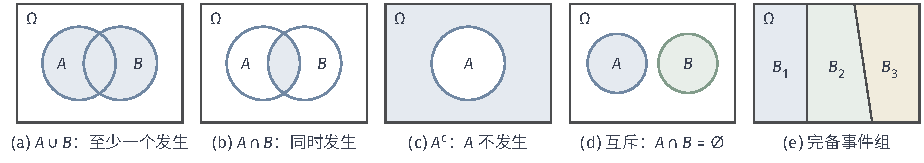
\includegraphics[width=156.5mm]{figures/01-basic-mathematics/05-probability-and-statistics-basics/tikz/prob-event-operations/figure.pdf}
  \caption{事件运算的集合示意。矩形表示样本空间$\Omega$，圆或分块表示事件，阴影是相应运算得到的事件。(a)(b)(c)分别是并、交与补；(d)中两个事件没有公共结果，因而互斥；(e)中三块互不重叠且铺满$\Omega$，每次试验恰有一块发生。}
  \label{fig:prob-event-operations}
\end{figure*}

\subsection{概率的定义与运算}
\label{sec:prob-probability-rules}

\paragraph{概率的定义}
我们希望给每个事件$A$配一个数$\mathbb{P}(A)$，表示它发生的可能性大小。直观上，这个数应当像“在大量重复试验中$A$发生的比例”那样运算：比例不会是负数，必然事件的比例是$1$，两个互斥事件合起来的比例等于各自比例之和。下面的定义只保留这三条规则，并把最后一条推广到可数个事件。

\begin{definition}[概率]
\label{def:prob-probability}
设对所讨论的每个事件$A$都给定一个实数$\mathbb{P}(A)$。若它满足
\begin{enumerate}
  \item 非负性：$\mathbb{P}(A)\geq0$；
  \item 归一性：$\mathbb{P}(\Omega)=1$；
  \item 可数可加性：对两两互斥的事件$A_1,A_2,\dots$，有$\mathbb{P}\bigl(\bigcup_{i\geq1}A_i\bigr)=\sum_{i\geq1}\mathbb{P}(A_i)$，
\end{enumerate}
就称$\mathbb{P}$为\term{概率}（probability），$\mathbb{P}(A)$为事件$A$的概率。
\end{definition}

第三条中的级数各项非负，它的和与求和次序无关（第~\ref{sec:ru-series-rearrangement-grouping}节）。为什么要求可数个而不只是有限个？等待时间问题中，“等待超过$10$分钟”可以拆成“等待落在$(10,11]$”“落在$(11,12]$”等可数个互斥事件之并；只有可数可加性，才能保证把这些片段的概率加起来得到整体的概率。

\paragraph{由定义推出的运算规则}
三条规则已经足以推出日常计算所需的公式。

\begin{theorem}[概率的基本性质]
\label{thm:prob-basic-properties}
设$A,B$为事件，则
\begin{enumerate}
  \item $\mathbb{P}(\varnothing)=0$，且对两两互斥的有限个事件有$\mathbb{P}(A_1\cup\dots\cup A_n)=\sum_{i=1}^n\mathbb{P}(A_i)$；
  \item 补事件公式：$\mathbb{P}(A^{\mathsf c})=1-\mathbb{P}(A)$；
  \item 单调性：若$A\subseteq B$，则$\mathbb{P}(B\setminus A)=\mathbb{P}(B)-\mathbb{P}(A)$，从而$\mathbb{P}(A)\leq\mathbb{P}(B)\leq1$；
  \item 加法公式：$\mathbb{P}(A\cup B)=\mathbb{P}(A)+\mathbb{P}(B)-\mathbb{P}(A\cap B)$，从而$\mathbb{P}(A\cup B)\leq\mathbb{P}(A)+\mathbb{P}(B)$。
\end{enumerate}
\end{theorem}
\begin{proof}
取$A_1=\Omega$、$A_i=\varnothing$（$i\geq2$），它们两两互斥，可数可加性给出$1=1+\sum_{i\geq2}\mathbb{P}(\varnothing)$；各项非负，只能$\mathbb{P}(\varnothing)=0$。把有限个互斥事件后面补上无穷多个空集，再用可数可加性，便得到有限可加性。

$A$与$A^{\mathsf c}$互斥且并为$\Omega$，有限可加性给出$\mathbb{P}(A)+\mathbb{P}(A^{\mathsf c})=1$。若$A\subseteq B$，则$B=A\cup(B\setminus A)$是互斥的并，于是$\mathbb{P}(B)=\mathbb{P}(A)+\mathbb{P}(B\setminus A)\geq\mathbb{P}(A)$；取$B=\Omega$即得$\mathbb{P}(A)\leq1$。

最后，$A\cup B$可以写成互斥的三块$A\setminus B$、$A\cap B$、$B\setminus A$之并，而$A$是前两块之并，$B$是后两块之并。分别对三者用有限可加性，便有$\mathbb{P}(A\cup B)=\mathbb{P}(A)+\mathbb{P}(B)-\mathbb{P}(A\cap B)$。
\end{proof}

加法公式减去$\mathbb{P}(A\cap B)$，是因为两块的公共部分被$\mathbb{P}(A)$与$\mathbb{P}(B)$各算了一次；它是第~\ref{chap:counting}章容斥原理的概率版本。丢掉这一项得到的不等式，对事件个数归纳后可推广到多个事件：$\mathbb{P}(A_1\cup\dots\cup A_n)\leq\sum_i\mathbb{P}(A_i)$，称为\term{联合界}（union bound）。它不要求事件互斥或有任何关系，因而常用来控制“至少有一处出错”的概率。补事件公式则提示一种常用的计算策略：“至少一个”往往不如它的反面“一个也没有”好算。

\paragraph{有限等可能模型}
若样本空间有限，并且根据试验的对称性认为每个样本点出现的可能性相同，就得到\term{古典概型}（classical probability model）：
\[
  \mathbb{P}(A)=\frac{|A|}{|\Omega|},
\]
其中$|A|$表示集合$A$的元素个数。概率计算由此化为计数。可以验证它满足概率的三条规则：比值非负，$|\Omega|/|\Omega|=1$，互斥事件的元素个数可以相加。

等可能性是我们对试验作出的模型假设，不是从样本空间推出的结论。公平骰子的六个面对称，所以取每面概率$1/6$；但如果把“两枚骰子的点数和”作为样本点，取值$2,3,\dots,12$并不等可能：和为$2$只有一种出法$(1,1)$，和为$7$却有六种。正确的做法是以有序对$(i,j)$为样本点，$36$个有序对等可能，于是点数和为$7$的概率是$6/36=1/6$，为$2$的概率只有$1/36$。

\begin{example}[抽检中至少一件次品]
\label{ex:prob-inspection-hypergeometric}
一批产品共$100$件，其中$5$件为次品。随机抽取$10$件且不放回，“随机”指$\binom{100}{10}$个$10$件子集等可能。样本中没有次品，等价于$10$件全部取自$95$件合格品，共有$\binom{95}{10}$种取法，所以
\[
  \mathbb{P}(\text{没有次品})=\frac{\binom{95}{10}}{\binom{100}{10}}
  =\frac{95\cdot94\cdots86}{100\cdot99\cdots91}\approx0.5838 .
\]
由补事件公式，至少抽到一件次品的概率约为$1-0.5838=0.4162$。也就是说，即使这批产品有$5\%$的次品，抽检$10$件仍有超过一半的可能一件次品也查不出来。
\end{example}

\paragraph{概率的连续性}
等待时间问题中，事件“$T<10$”可以由一列事件“$T\leq10-1/n$”逐步逼近，事件“$T\leq10$”也是“$T\leq10+1/n$”逐步收缩的极限。我们希望概率随事件的这种单调逼近而连续变化。若$A_1\subseteq A_2\subseteq\cdots$且$A=\bigcup_nA_n$，记作$A_n\uparrow A$；若$A_1\supseteq A_2\supseteq\cdots$且$A=\bigcap_nA_n$，记作$A_n\downarrow A$。

\begin{theorem}[概率的连续性]
\label{thm:prob-continuity}
若$A_n\uparrow A$，则$\mathbb{P}(A_n)\to\mathbb{P}(A)$；若$A_n\downarrow A$，同样有$\mathbb{P}(A_n)\to\mathbb{P}(A)$。
\end{theorem}
\begin{proof}
设$A_n\uparrow A$。令$B_1=A_1$，$B_n=A_n\setminus A_{n-1}$（$n\geq2$），即$B_n$是第$n$步新增加的部分。这些$B_n$两两互斥，$A_n=B_1\cup\dots\cup B_n$，且$A=\bigcup_{n\geq1}B_n$。由可数可加性与有限可加性，
\[
  \mathbb{P}(A)=\sum_{k=1}^{\infty}\mathbb{P}(B_k)
  =\lim_{n\to\infty}\sum_{k=1}^{n}\mathbb{P}(B_k)
  =\lim_{n\to\infty}\mathbb{P}(A_n).
\]
若$A_n\downarrow A$，则补事件满足$A_n^{\mathsf c}\uparrow A^{\mathsf c}$（De Morgan律），由前一结论$\mathbb{P}(A_n^{\mathsf c})\to\mathbb{P}(A^{\mathsf c})$，再用补事件公式即得。
\end{proof}

证明中递减情形借助了补事件，这里用到$\mathbb{P}(\Omega)=1$有限。连续性是可数可加性的直接推论；下一节将用它说明分布函数为什么右连续，以及单点概率怎样由分布函数的跳跃读出。

\subsection{条件概率}
\label{sec:prob-conditional-probability}

\paragraph{定义与直观}
掷一枚公平骰子，“点数不小于$4$”的概率是$1/2$。若有人告诉我们这次出现的是偶数点，可能的结果就只剩$\{2,4,6\}$，其中$4$和$6$两个满足条件，可能性变成$2/3$。已知信息把考虑范围从$\Omega$缩小到事件$B$，再在$B$内部按原来的相对大小重新分配概率。

\begin{definition}[条件概率]
\label{def:prob-conditional-probability}
设$\mathbb{P}(B)>0$。事件$A$在事件$B$发生条件下的\term{条件概率}（conditional probability）定义为
\[
  \mathbb{P}(A\mid B)=\frac{\mathbb{P}(A\cap B)}{\mathbb{P}(B)} .
\]
\end{definition}

分子只保留$A$中同时落在$B$内的部分，分母$\mathbb{P}(B)$把$B$的总概率重新标定为$1$。在古典概型中，它就是$|A\cap B|/|B|$，即只在$B$内部计数。固定$B$后，$A\mapsto\mathbb{P}(A\mid B)$本身满足概率的三条规则，因此前面的补事件公式、加法公式等都可以在条件之下照用。定义要求$\mathbb{P}(B)>0$：以零概率事件为条件需要另外的构造，本节不讨论；对连续取值变量取条件的问题，留到第~\ref{sec:rvec-conditioning}节用条件密度处理。

\paragraph{乘法公式}
把定义式两边乘以$\mathbb{P}(B)$，得到\term{乘法公式}（multiplication rule）
\[
  \mathbb{P}(A\cap B)=\mathbb{P}(B)\,\mathbb{P}(A\mid B).
\]
它适合按时间顺序计算：先算第一步的概率，再乘以在第一步结果已知时第二步的条件概率。对多个事件反复使用，只要各个条件事件的概率为正，就有
\[
  \mathbb{P}(A_1\cap A_2\cap\dots\cap A_n)
  =\mathbb{P}(A_1)\,\mathbb{P}(A_2\mid A_1)\cdots\mathbb{P}(A_n\mid A_1\cap\dots\cap A_{n-1}).
\]

\begin{example}[不放回抽球]
\label{ex:prob-urn-without-replacement}
袋中有$3$个红球、$2$个白球，依次不放回地摸出两个。记$R_1$、$R_2$分别为第一、二次摸到红球。第一次摸到红球后袋中剩$2$红$2$白，所以$\mathbb{P}(R_2\mid R_1)=2/4$；第一次摸到白球后剩$3$红$1$白，所以$\mathbb{P}(R_2\mid R_1^{\mathsf c})=3/4$。由乘法公式，
\[
  \mathbb{P}(R_1\cap R_2)=\frac35\cdot\frac24=\frac{3}{10},\qquad
  \mathbb{P}(R_1^{\mathsf c}\cap R_2)=\frac25\cdot\frac34=\frac{3}{10}.
\]
两者互斥且并为$R_2$，故$\mathbb{P}(R_2)=3/5$，与第一次摸到红球的概率相同。

不放回时，第一次的结果改变了第二次的条件概率：$1/2$与$3/4$都不等于$3/5$。若每次摸完放回，袋中构成不变，无论第一次摸到什么，第二次摸到红球的条件概率都是$3/5$。条件是否改变后续概率，正是下一小节要刻画的独立性。
\end{example}

\subsection{事件的独立性}
\label{sec:prob-event-independence}

\paragraph{两个事件的独立}
放回抽球时，第一次的结果不改变第二次的概率：$\mathbb{P}(R_2\mid R_1)=\mathbb{P}(R_2)$。把这一等式乘以$\mathbb{P}(R_1)$，就得到对称的乘积形式，它在$\mathbb{P}(R_1)=0$时也有意义。

\begin{definition}[事件的独立性]
\label{def:prob-independent-events}
若$\mathbb{P}(A\cap B)=\mathbb{P}(A)\,\mathbb{P}(B)$，就称事件$A$与$B$\term{相互独立}（independent）。
\end{definition}

当$\mathbb{P}(B)>0$时，独立等价于$\mathbb{P}(A\mid B)=\mathbb{P}(A)$，即知道$B$发生并不改变$A$的概率。若$A$与$B$独立，则$A$与$B^{\mathsf c}$也独立：$\mathbb{P}(A\cap B^{\mathsf c})=\mathbb{P}(A)-\mathbb{P}(A\cap B)=\mathbb{P}(A)(1-\mathbb{P}(B))=\mathbb{P}(A)\mathbb{P}(B^{\mathsf c})$。“$B$发生”不提供关于$A$的信息，“$B$不发生”同样不提供。

独立性是关于概率数值的条件，要按定义核对，不能凭事件“看起来无关”判断。掷一枚公平骰子，令$A=\{2,4,6\}$，$B=\{1,2\}$，$C=\{1,2,3\}$。$\mathbb{P}(A\cap B)=\mathbb{P}(\{2\})=1/6=\frac12\cdot\frac13$，所以$A$与$B$独立；$\mathbb{P}(A\cap C)=1/6\neq\frac12\cdot\frac12$，所以$A$与$C$不独立。独立也不同于互斥：若$\mathbb{P}(A),\mathbb{P}(B)>0$且$A,B$互斥，则$\mathbb{P}(A\cap B)=0<\mathbb{P}(A)\mathbb{P}(B)$，知道$B$发生就确知$A$不发生，二者并不独立。

\paragraph{多个事件的相互独立}
三个以上事件的独立性要更小心。我们希望任意几个事件的发生情况都不影响其余事件，这需要所有子组都满足乘法关系。

\begin{definition}[多个事件的相互独立]
\label{def:prob-mutual-independence}
称事件$A_1,\dots,A_n$相互独立（mutually independent），若对任意$2\leq k\leq n$和任意下标$1\leq i_1<\dots<i_k\leq n$，都有
\[
  \mathbb{P}(A_{i_1}\cap\dots\cap A_{i_k})=\mathbb{P}(A_{i_1})\cdots\mathbb{P}(A_{i_k}).
\]
\end{definition}

只验证两两之间的乘法关系是不够的。

\begin{example}[两两独立但不相互独立]
\label{ex:prob-pairwise-not-mutual}
抛两枚公平硬币，四个结果等可能。令$A$为“第一枚正面”，$B$为“第二枚正面”，$C$为“两枚结果相同”。每个事件的概率都是$1/2$，任意两个同时发生的概率都是$1/4$（例如$A\cap C$就是“两枚都正面”），所以三对事件都独立。但$A\cap B$发生时$C$必然发生，$\mathbb{P}(A\cap B\cap C)=1/4\neq1/8$，三者不相互独立：知道$A$与$B$，就完全知道了$C$。
\end{example}

相互独立的定义为“独立重复试验”给出了明确条件。设一项试验重复$n$次，$A_i$是只依赖第$i$次结果的事件（例如“第$i$次成功”）。若$A_1,\dots,A_n$相互独立，且$\mathbb{P}(A_i)=p$，则$n$次全部成功的概率是$p^n$，前$k$次成功、其余失败的概率是$p^k(1-p)^{n-k}$（独立性对补事件保持，可以把其中任意几个$A_i$换成补事件）。第~\ref{sec:prob-discrete-models}节的二项分布与几何分布都建立在这个条件上。

\section{随机变量与概率分布}
\label{sec:prob-distributions}

抽检关心次品的“个数”，排队关心等待的“分钟数”。我们常常不需要试验结果的全部细节，只需要由结果算出的一个数。本节把这种“结果到数值”的对应写成随机变量，并研究怎样完整描述它取各种值的概率。

\subsection{随机变量与实现值}
\label{sec:prob-random-variables}

\paragraph{随机变量}
抽检的样本点是一个$10$件子集，而我们关心的是其中次品的个数；这个个数由样本点完全确定，但样本点本身是随机的。把每个结果对应到一个实数的规则，就是随机变量。

\begin{definition}[随机变量]
\label{def:prob-random-variable}
定义在样本空间上的实值函数$X:\Omega\to\mathbb{R}$称为\term{随机变量}（random variable）。对实数集的子集$B$，记
\[
  \{X\in B\}=\{\omega\in\Omega: X(\omega)\in B\},
\]
它是一个事件，其概率记作$\mathbb{P}(X\in B)$。
\end{definition}

本部分默认所讨论的$\{X\in B\}$（$B$为区间或单点等）都是可以赋予概率的事件；一般的可测性要求见\BookPartRef{part:probability-spaces}{卷2《数学准备：抽象数学》的“概率空间”部分}。随机变量本身是一个确定的函数，随机性来自样本点$\omega$的出现。我们把随机变量记成大写字母$X$，它的可能取值组成集合$X(\Omega)$；一次试验出现结果$\omega$后，得到的具体数$x=X(\omega)$称为$X$的一个\term{实现值}（realization），用小写字母表示。例如“$X\leq3$”是一个事件，而“$x=2$”是一次观测的结果。

\paragraph{分布由映射与概率共同决定}
同一次试验可以定义多个随机变量。掷一枚骰子，$\Omega=\{1,\dots,6\}$，令$X(\omega)=\omega$为点数，令
\[
  I(\omega)=\begin{cases}1,&\omega\text{为偶数},\\0,&\omega\text{为奇数}.\end{cases}
\]
$I$只记录点数的奇偶。一般地，对事件$A$，称取值$1$（$\omega\in A$）或$0$（$\omega\notin A$）的函数$\mathbb{I}_A$为$A$的\term{指示函数}（indicator function），于是$I=\mathbb{I}_{\{2,4,6\}}$。图~\ref{fig:prob-die-indicator-map}画出了两个变量的对应关系：$X$把六个结果送到六个不同的值，$I$则把三个偶数结果合并到$1$，三个奇数结果合并到$0$。

\begin{figure}[htbp]
  \centering
  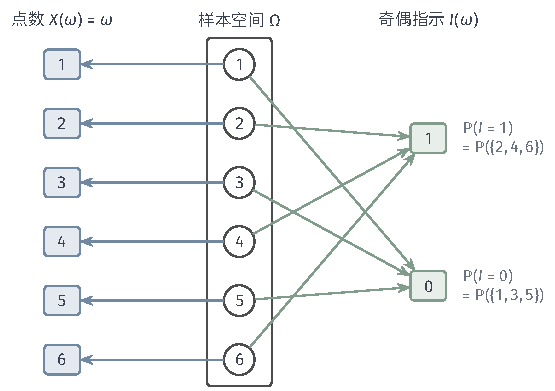
\includegraphics[width=94mm]{figures/01-basic-mathematics/05-probability-and-statistics-basics/tikz/prob-die-indicator-map/figure.pdf}
  \caption{同一次掷骰试验上的两个随机变量。中间是样本空间的六个结果；左侧的点数$X$把每个结果送到不同的值，右侧的奇偶指示变量$I$把三个偶数结果都送到$1$、三个奇数结果都送到$0$。$I$取某个值的概率，等于被送到该值的全部结果的概率之和。}
  \label{fig:prob-die-indicator-map}
\end{figure}

要知道$I$取$1$的概率，就把被送到$1$的结果的概率加起来：$\mathbb{P}(I=1)=\mathbb{P}(\{2,4,6\})$。骰子公平时它等于$1/2$。若骰子被做了手脚，$\mathbb{P}(\{6\})=1/2$，其余五面各为$1/10$，同一个函数$I$给出$\mathbb{P}(I=1)=0.1+0.1+0.5=0.7$。可见随机变量取值的概率规律既取决于对应规则$X$，也取决于试验结果上的概率$\mathbb{P}$。

\begin{definition}[分布]
\label{def:prob-distribution}
随机变量$X$的\term{分布}（distribution）是指对实数集的各个子集$B$给出概率$\mathbb{P}(X\in B)$的对应关系$B\mapsto\mathbb{P}(X\in B)$，也记作$P_X(B)$。
\end{definition}

分布只记录“取值落在哪里的概率”，不再记录是哪个结果导致了这个取值。不同的随机变量可以有相同的分布：公平骰子上的$I$与$1-I$（奇数指示）都以概率$1/2$取$0$和$1$，但在每次试验中二者的取值恰好相反。所以“分布相同”与“随机变量相等”是两回事；两个随机变量$X,Y$分布相同时，记作$X\overset{d}{=}Y$，以区别于逐个结果都相等的$X=Y$。

\subsection{分布函数}
\label{sec:prob-cdf}

\paragraph{定义与性质}
分布要对很多集合给出概率，逐一列出并不现实。对实值随机变量，只需记录形如$(-\infty,x]$的半直线的概率，其余区间的概率就能由它们相减得到。

\begin{definition}[分布函数]
\label{def:prob-cdf}
随机变量$X$的\term{分布函数}（distribution function，也称累积分布函数，cumulative distribution function，CDF）定义为
\[
  F_X(x)=\mathbb{P}(X\leq x),\qquad x\in\mathbb{R}.
\]
\end{definition}

对$a<b$，事件$\{X\leq b\}$是互斥的$\{X\leq a\}$与$\{a<X\leq b\}$之并，因此
\[
  \mathbb{P}(a<X\leq b)=F_X(b)-F_X(a).
\]
左开右闭的区间与分布函数的“$\leq$”配套。其他类型区间的概率还需要知道单点概率，这由下面的性质给出。

\begin{theorem}[分布函数的性质]
\label{thm:prob-cdf-properties}
任一随机变量的分布函数$F=F_X$满足：
\begin{enumerate}
  \item 单调不减：$x<y$时$F(x)\leq F(y)$；
  \item 右连续：$\lim_{y\downarrow x}F(y)=F(x)$；
  \item 两端极限：$\lim_{x\to-\infty}F(x)=0$，$\lim_{x\to+\infty}F(x)=1$。
\end{enumerate}
此外，左极限$F(x^-)=\lim_{y\uparrow x}F(y)$存在，且$F(x^-)=\mathbb{P}(X<x)$，$\mathbb{P}(X=x)=F(x)-F(x^-)$。
\end{theorem}
\begin{proof}
$x<y$时$\{X\leq x\}\subseteq\{X\leq y\}$，单调性由概率的单调性得到。单调函数的单侧极限总存在，所以只需沿特殊数列计算极限。

取$y_n=x+1/n$，事件$\{X\leq y_n\}$递减，交集为$\{X\leq x\}$，由概率的连续性$F(y_n)\to F(x)$，这就是右连续。同理，$\{X\leq -n\}\downarrow\varnothing$，$\{X\leq n\}\uparrow\Omega$，分别给出两端极限$0$与$1$。

最后取$y_n=x-1/n$，事件$\{X\leq y_n\}$递增，并集是$\{X<x\}$（不含$x$本身），所以$F(x^-)=\mathbb{P}(X<x)$。$\{X\leq x\}$是$\{X<x\}$与$\{X=x\}$的互斥并，相减即得单点概率。
\end{proof}

右连续而不一定左连续的原因在于“$\leq$”包含端点：从右侧逼近$x$的事件交出$\{X\leq x\}$，从左侧逼近的事件并出$\{X<x\}$，二者相差的正是单点$\{X=x\}$。于是分布函数在$x$处的跳跃高度等于$\mathbb{P}(X=x)$，而$F$在$x$连续当且仅当$\mathbb{P}(X=x)=0$。有了单点概率，$\mathbb{P}(a\leq X\leq b)=F(b)-F(a^-)$等各类区间的概率都能写出。反过来也成立：任何满足上述三条性质的函数，都是某个随机变量的分布函数，并且分布函数唯一确定分布；这一结论的证明需要一般测度构造，留到\BookPartRef{part:probability-spaces}{卷2《数学准备：抽象数学》的“概率空间”部分}。

\paragraph{三类分布函数}
分布函数对所有实值随机变量都有定义，因而能用同一种语言描述取值方式很不相同的变量。下面三个例子对应图~\ref{fig:prob-cdf-three-types}的三幅子图。

\begin{figure*}[htbp]
  \centering
  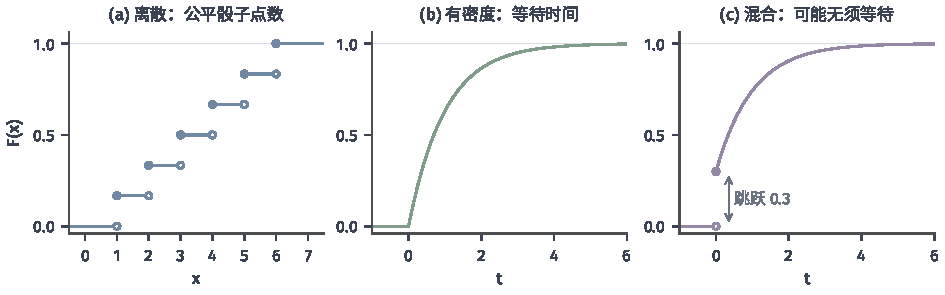
\includegraphics[width=160mm]{figures/01-basic-mathematics/05-probability-and-statistics-basics/matplotlib/prob-cdf-three-types/figure.pdf}
  \caption{三类分布函数。(a)公平骰子的点数，分布函数是阶梯函数，在$1,\dots,6$各跳$1/6$，实心点表示取到的函数值、空心点表示左极限；(b)等待时间$T$满足$F(t)=1-e^{-t}$（$t\geq0$），曲线连续；(c)以概率$0.3$无须等待、否则等待时间按(b)的规律分布，曲线在$0$处跳跃$0.3$，之后连续上升。三条曲线都单调不减、右连续，并从$0$升到$1$。}
  \label{fig:prob-cdf-three-types}
\end{figure*}

\begin{example}[离散、连续与混合]
\label{ex:prob-three-cdfs}
(a)公平骰子的点数$X$：$x<1$时$F_X(x)=0$，$k\leq x<k+1$（$k=1,\dots,5$）时$F_X(x)=k/6$，$x\geq6$时$F_X(x)=1$。函数在每个整数点$k$跳跃$1/6$，在两个整数之间保持水平。

(b)等待时间$T$满足$F_T(t)=0$（$t<0$）、$F_T(t)=1-e^{-t}$（$t\geq0$），以分钟计。它处处连续，所以每个单点的概率都是$0$；等待超过$2$分钟的概率是$1-F_T(2)=e^{-2}\approx0.135$。

(c)设窗口空闲时（概率$0.3$）顾客无须等待，否则等待时间按(b)的规律分布。于是
\[
  F_W(t)=\begin{cases}0,&t<0,\\0.3+0.7(1-e^{-t}),&t\geq0.\end{cases}
\]
函数在$0$处跳跃$0.3$，即$\mathbb{P}(W=0)=0.3$；在$t>0$上连续上升。
\end{example}

例(a)的变量只取有限个值，概率全部集中在这些点上；例(b)的变量没有任何单点带正概率；例(c)两者兼有。接下来的两小节分别为前两类给出更方便的表示：概率质量函数和概率密度函数。例(c)说明这两类并不覆盖全部情形，此时分布函数仍然适用，计算可以把跳跃部分求和、连续部分积分。

\subsection{概率质量函数}
\label{sec:prob-pmf}

\paragraph{定义与计算}
骰子点数、次品个数这类变量只取有限或可数多个值。对它们而言，最直接的描述是逐个列出每个取值的概率。

\begin{definition}[离散随机变量与概率质量函数]
\label{def:prob-pmf}
若存在有限或可数的集合$\{x_1,x_2,\dots\}$使$\mathbb{P}(X\in\{x_1,x_2,\dots\})=1$，就称$X$为\term{离散随机变量}（discrete random variable）。函数
\[
  p_X(x)=\mathbb{P}(X=x),\qquad x\in\mathbb{R}
\]
称为$X$的\term{概率质量函数}（probability mass function，PMF）。
\end{definition}

质量函数满足$p_X(x)\geq0$，只在可能取值处为正，且$\sum_ip_X(x_i)=1$。对任意集合$B$，事件$\{X\in B\}$是可数个互斥单点事件$\{X=x_i\}$（$x_i\in B$）之并，由可数可加性
\[
  \mathbb{P}(X\in B)=\sum_{x_i\in B}p_X(x_i).
\]
反过来，任给可数个点和满足非负、总和为$1$的一组数，都能定义一个离散分布。离散分布的计算因而就是求和。

\begin{example}[三次抛硬币的正面数]
\label{ex:prob-three-coins}
抛三枚公平硬币，令$X$为正面个数。$8$个结果等可能，含$k$个正面的结果有$\binom{3}{k}$个，所以
\[
  p_X(0)=\tfrac18,\quad p_X(1)=\tfrac38,\quad p_X(2)=\tfrac38,\quad p_X(3)=\tfrac18 .
\]
“至少一次正面”的概率是$p_X(1)+p_X(2)+p_X(3)=7/8$，也可以用补事件写成$1-p_X(0)$。
\end{example}

\paragraph{质量函数与分布函数}
离散变量的分布函数是质量函数的累加：
\[
  F_X(x)=\sum_{x_i\leq x}p_X(x_i).
\]
因此$F_X$是阶梯函数，跳跃发生在可能取值$x_i$处，跳跃高度就是$p_X(x_i)$，这正是定理~\ref{thm:prob-cdf-properties}中$\mathbb{P}(X=x)=F(x)-F(x^-)$的具体形式。图~\ref{fig:prob-pmf-cdf}把例~\ref{ex:prob-three-coins}的两种表示并排画出：左图的竖线高度，正是右图对应台阶的高度差。

\begin{figure}[htbp]
  \centering
  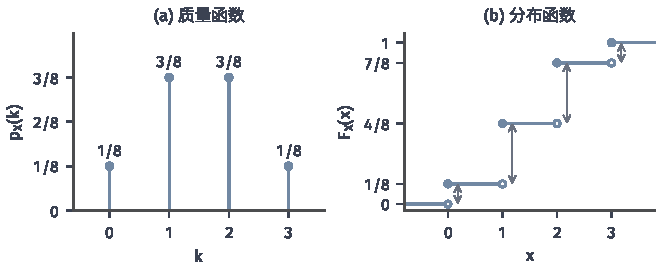
\includegraphics[width=112mm]{figures/01-basic-mathematics/05-probability-and-statistics-basics/matplotlib/prob-pmf-cdf/figure.pdf}
  \caption{三次抛公平硬币的正面数。(a)概率质量函数，竖线高度是各取值的概率；(b)分布函数，箭头标出每个台阶的跳跃高度，依次为$1/8,3/8,3/8,1/8$，与(a)的竖线一一对应。两次跳跃之间分布函数保持水平，因为那里没有可能取值。}
  \label{fig:prob-pmf-cdf}
\end{figure}

两种表示可以互相转换：从质量函数累加得到分布函数，从分布函数读出各处的跳跃得到质量函数。计算区间概率时，分布函数往往更快：$\mathbb{P}(1\leq X\leq2)=F_X(2)-F_X(1^-)=F_X(2)-F_X(0)=7/8-1/8=3/4$。注意这里用的是$F_X(1^-)$而不是$F_X(1)$，因为区间包含左端点$1$，而$1$处恰有正概率。

\subsection{概率密度函数}
\label{sec:prob-pdf}

\paragraph{用积分计算概率}
等待时间的每个单点概率都是$0$，质量函数不能提供任何信息。此时我们改用“单位长度上的概率”来描述：概率像质量一样沿数轴连续分布，区间上的概率是密度在该区间上的积分。

\begin{definition}[概率密度函数]
\label{def:prob-pdf}
若存在非负函数$f_X$，使$\int_{-\infty}^{\infty}f_X(x)\,\mathrm{d}x=1$，并且对一切$a<b$都有
\[
  \mathbb{P}(a<X\leq b)=\int_a^b f_X(x)\,\mathrm{d}x,
\]
就称$X$具有\term{概率密度函数}（probability density function，PDF）$f_X$，简称密度。
\end{definition}

这里的积分可以是第~\ref{sec:ru-improper-integrals}节的反常积分，$a$也可以取$-\infty$。有密度的变量满足$\mathbb{P}(X=x)=0$：分布函数$F_X(x)=\int_{-\infty}^xf_X(t)\,\mathrm{d}t$是积分上限函数，处处连续，而由定理~\ref{thm:prob-cdf-properties}，单点概率就是分布函数在该点的跳跃高度。因此$\mathbb{P}(a<X\leq b)$、$\mathbb{P}(a\leq X\leq b)$、$\mathbb{P}(a<X<b)$都相等，端点开闭不影响结果。

密度值不是概率。若$f_X$在$x$处连续，由积分中值定理，
\[
  \mathbb{P}(x<X\leq x+h)=\int_x^{x+h}f_X(t)\,\mathrm{d}t\approx f_X(x)\,h,
\]
更准确地说，中值定理给出$\int_x^{x+h}f_X=f_X(\xi_h)h$，其中$\xi_h\in[x,x+h]$，由连续性$f_X(\xi_h)\to f_X(x)$。所以$f_X(x)$是“小区间上的概率除以区间长度”的极限，单位是“概率每单位长度”。它可以大于$1$，只要乘上区间长度后的累计不超过$1$。

\begin{example}[密度值大于一]
\label{ex:prob-density-above-one}
设$X$在$(0,1/2)$上取值，且等长子区间等可能，则$f_X(x)=2$（$0<x<1/2$），其余处为$0$。密度处处等于$2$，但$\mathbb{P}(0.1<X\leq0.3)=2\times0.2=0.4$。又设等待时间$T$的密度为$f_T(t)=3e^{-3t}$（$t\geq0$），则$f_T(0)=3$，而$\mathbb{P}(0<T\leq0.2)=1-e^{-0.6}\approx0.451$。图~\ref{fig:prob-density-above-one}画出这两个密度，阴影面积就是所求概率。
\end{example}

\begin{figure}[htbp]
  \centering
  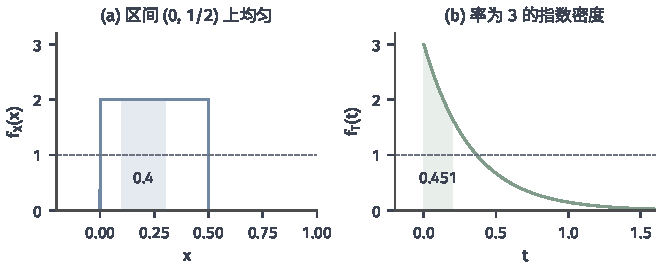
\includegraphics[width=112mm]{figures/01-basic-mathematics/05-probability-and-statistics-basics/matplotlib/prob-density-above-one/figure.pdf}
  \caption{密度值可以大于一。(a)区间$(0,1/2)$上的均匀密度恒为$2$，阴影是$\mathbb{P}(0.1<X\leq0.3)=0.4$；(b)率为$3$的指数密度在$0$处等于$3$，阴影是$\mathbb{P}(0<T\leq0.2)\approx0.451$。虚线标出高度$1$。概率由面积给出，曲线的高度只表示单位长度上的概率。}
  \label{fig:prob-density-above-one}
\end{figure}

\paragraph{密度与分布函数}
取$a\to-\infty$，定义直接给出分布函数是密度的累计：
\[
  F_X(x)=\int_{-\infty}^{x}f_X(t)\,\mathrm{d}t .
\]
由微积分基本定理（定理~\ref{thm:ru-accumulation-derivative}），在$f_X$连续的点有$F_X'(x)=f_X(x)$：密度是分布函数的变化率。反过来，若$F_X$连续，并且除有限个点外连续可微，那么$f_X=F_X'$（在那有限个点处任意取值）就是一个密度，因为由Newton--Leibniz公式，每段上$F_X$的增量都等于$F_X'$的积分，而有限个点不影响积分。例如$F_X(x)=x^2$（$0\leq x\leq1$）连同两侧的$0$与$1$，给出密度$f_X(x)=2x$（$0<x<1$）。

密度只在积分意义下确定：改变有限个点处的函数值，所有区间上的积分都不变，所以两个密度若只在有限个点不同，描述的是同一个分布。另一方面，“分布函数连续”还不足以保证密度存在。有连续分布函数的变量所有单点概率为零，但仍可能把全部概率集中在一个“总长度为零”的集合上；Cantor函数就是这样的例子，它连续、单调地从$0$升到$1$，导数却在除一个零长度集合外的所有点都等于零，任何密度的积分都无法还原它。这类分布在应用中很少直接出现，但它说明离散分布与有密度的分布并未穷尽所有情形，例~\ref{ex:prob-three-cdfs}(c)的混合分布也不属于这两类。

\section{分布的数值特征}
\label{sec:prob-numerical-features}

分布函数、质量函数和密度保存了分布的全部信息，但回答“平均要等多久”“波动有多大”这类问题时，我们需要的是一两个数。本节用期望描述平均位置，用方差描述围绕平均的波动，用分位数描述累计概率对应的位置，再用高阶矩补充形状信息。

\subsection{期望}
\label{sec:prob-expectation}

\paragraph{定义与可积条件}
掷一枚公平骰子很多次，点数的平均值会稳定在什么地方？每个点数出现的比例约为$1/6$，平均值就约为$\sum_{k=1}^6k\cdot\frac16=3.5$。这个计算把每个可能取值按其概率加权平均，它不依赖任何一次的具体结果。重复次数增加时样本平均为何会接近这个数，是第~\ref{sec:samp-lln}节大数定律的内容；这里先把加权平均本身定义清楚。

\begin{definition}[期望]
\label{def:prob-expectation}
设$X$为离散随机变量，质量函数为$p_X$。若级数$\sum_i|x_i|\,p_X(x_i)$收敛，定义$X$的\term{期望}（expectation）为
\[
  \mathbb{E}[X]=\sum_ix_i\,p_X(x_i).
\]
设$X$具有密度$f_X$。若$\int_{-\infty}^{\infty}|x|\,f_X(x)\,\mathrm{d}x<\infty$，定义
\[
  \mathbb{E}[X]=\int_{-\infty}^{\infty}x\,f_X(x)\,\mathrm{d}x .
\]
满足相应条件时，称$X$的期望有限，或称$X$\term{可积}（integrable）。期望也称\term{均值}（mean），常记作$\mu$或$\mu_X$。
\end{definition}

定义先要求绝对值的加权和有限，是因为可数个取值可能有正有负。若只是条件收敛，第~\ref{sec:ru-series-rearrangement-grouping}节已经说明重排求和次序可以改变级数的和，而可能取值并没有天然的先后次序；绝对收敛保证无论按什么次序相加结果都一样。对非负变量，加权和要么有限、要么为$+\infty$，此时可以写$\mathbb{E}[X]=+\infty$；对一般变量，绝对值的和无穷时期望没有定义。

\begin{example}[期望不存在的分布]
\label{ex:prob-infinite-expectation}
设$X$取正整数，$p_X(k)=\frac{1}{k(k+1)}$。由$\frac{1}{k(k+1)}=\frac1k-\frac1{k+1}$，部分和逐项相消，$\sum_{k\geq1}p_X(k)=1$，这是一个合法的分布。但$\sum_kk\,p_X(k)=\sum_k\frac{1}{k+1}=+\infty$，所以$\mathbb{E}[X]=+\infty$：大的取值概率虽小，衰减却不够快。连续情形的例子是Cauchy密度$f(x)=\frac{1}{\pi(1+x^2)}$，它关于$0$对称，但$\int|x|f(x)\,\mathrm{d}x=+\infty$，期望没有定义，不能凭对称性说期望等于$0$。
\end{example}

例~\ref{ex:prob-three-cdfs}(c)的混合分布兼有跳跃与连续部分，其期望把两部分分别计算后相加：$\mathbb{E}[W]=0\times0.3+\int_0^\infty t\cdot0.7e^{-t}\,\mathrm{d}t=0.7$。一般分布统一的期望定义需要测度积分，留到\BookPartRef{part:probability-spaces}{卷2《数学准备：抽象数学》的“概率空间”部分}；本部分只用离散求和与密度积分。

\paragraph{函数的期望与线性性}
我们常常需要$X$的某个函数的平均，例如点数平方的平均，或观测加上噪声后的平均。按定义，似乎要先求出新变量$g(X)$的分布，再求加权平均。下面的结论说明这一步可以省去。

\begin{theorem}[函数的期望]
\label{thm:prob-lotus}
设$g$为实值函数。若$X$离散，且级数$\sum_i|g(x_i)|\,p_X(x_i)$收敛，则
\[
  \mathbb{E}[g(X)]=\sum_ig(x_i)\,p_X(x_i);
\]
若$X$有密度$f_X$，$g$分段连续且$\int|g(x)|f_X(x)\,\mathrm{d}x<\infty$，则
\begin{equation}
  \mathbb{E}[g(X)]=\int_{-\infty}^{\infty}g(x)\,f_X(x)\,\mathrm{d}x .
  \label{eq:prob-lotus}
\end{equation}
\end{theorem}
\begin{proof}
只证离散情形。$Y=g(X)$也是离散变量，它取值$y$当且仅当$X$取某个满足$g(x_i)=y$的$x_i$，所以$p_Y(y)=\sum_{i:\,g(x_i)=y}p_X(x_i)$。按$Y$的定义，
\[
  \mathbb{E}[Y]=\sum_yy\,p_Y(y)=\sum_y\sum_{i:\,g(x_i)=y}g(x_i)\,p_X(x_i)=\sum_ig(x_i)\,p_X(x_i).
\]
最后一步把双重和按$i$重新排列：每个$i$恰好出现在$y=g(x_i)$那一组中。绝对收敛的假设保证重排不改变和，同时也说明$Y$的期望有限。
\end{proof}

密度情形的证明需要知道$g(X)$的分布。第~\ref{sec:prob-density-change}节在$g$严格单调可微时用变量替换验证式~\eqref{eq:prob-lotus}；一般情形的证明留到\BookPartRef{part:probability-spaces}{卷2《数学准备：抽象数学》的“概率空间”部分}。例如公平骰子点数的平方，直接计算$\mathbb{E}[X^2]=\frac16(1+4+9+16+25+36)=\frac{91}{6}$，不必先列出$X^2$取$1,4,\dots,36$的分布。

由定理~\ref{thm:prob-lotus}与求和、积分的线性性，期望对函数的线性组合是线性的：只要$g(X)$与$h(X)$的期望都有限，对常数$a,b,c$有
\[
  \mathbb{E}[a\,g(X)+b\,h(X)+c]=a\,\mathbb{E}[g(X)]+b\,\mathbb{E}[h(X)]+c .
\]
特别地，$\mathbb{E}[aX+b]=a\,\mathbb{E}[X]+b$，常数的期望是它自己。多个不同随机变量之和的期望同样可以拆开，其证明要用到它们的联合分布，在第~\ref{sec:rvec-moments}节讨论。

\begin{example}[带噪观测的平均目标]
\label{ex:probability-noisy-observation}
用仪器测量一个固定的未知量$\theta$，读数为$Y=\theta+\varepsilon$，其中误差$\varepsilon$是随机变量，满足$\mathbb{E}[\varepsilon]=0$。$Y$是$\varepsilon$的函数$g(\varepsilon)=\theta+\varepsilon$，由线性性
\[
  \mathbb{E}[Y]=\theta+\mathbb{E}[\varepsilon]=\theta .
\]
这说明读数“平均而言”没有系统偏差，却不保证一次读数接近$\theta$。例如$\varepsilon$以各$1/2$的概率取$\pm10$，则$\mathbb{E}[Y]=\theta$，但每次读数都恰好偏离$\theta$十个单位。期望只描述平均位置；读数离$\theta$有多远，需要下一小节的方差来刻画，多次读数的平均能否接近$\theta$，则要等到第~\ref{chap:sampling-errors}章讨论。
\end{example}

\subsection{方差与标准差}
\label{sec:prob-variance}

\paragraph{定义与计算公式}
例~\ref{ex:probability-noisy-observation}中，误差取$\pm10$与取$\pm1$的期望都是$0$，读数的可靠程度却差别很大。要区分它们，需要衡量取值偏离均值的典型程度。偏差$X-\mu$有正有负，平均起来恰为零，所以我们取偏差的平方再平均。

\begin{definition}[方差与标准差]
\label{def:prob-variance}
设$\mathbb{E}[X^2]<\infty$，记$\mu=\mathbb{E}[X]$。$X$的\term{方差}（variance）定义为
\[
  \operatorname{Var}(X)=\mathbb{E}\bigl[(X-\mu)^2\bigr],
\]
其非负平方根$\sigma_X=\sqrt{\operatorname{Var}(X)}$称为\term{标准差}（standard deviation）。方差也常记作$\sigma^2$或$\sigma_X^2$。
\end{definition}

条件$\mathbb{E}[X^2]<\infty$称为二阶矩有限，它保证均值也有限：由$|x|\leq\frac12(1+x^2)$，$\mathbb{E}|X|\leq\frac12(1+\mathbb{E}[X^2])<\infty$。展开平方并用线性性，得到常用的计算公式
\[
  \operatorname{Var}(X)=\mathbb{E}[X^2]-2\mu\,\mathbb{E}[X]+\mu^2=\mathbb{E}[X^2]-\mu^2 .
\]
方差总是非负的，所以$\mathbb{E}[X^2]\geq(\mathbb{E}[X])^2$。方差为零意味着$X$以概率$1$等于常数$\mu$：对离散变量，$\sum_i(x_i-\mu)^2p_X(x_i)=0$要求每个正概率取值都等于$\mu$。

\begin{example}[骰子点数的方差]
\label{ex:prob-die-variance}
公平骰子的点数有$\mu=7/2$，$\mathbb{E}[X^2]=91/6$，于是
\[
  \operatorname{Var}(X)=\frac{91}{6}-\frac{49}{4}=\frac{182-147}{12}=\frac{35}{12}\approx2.92,
  \qquad \sigma_X\approx1.71 .
\]
对比例~\ref{ex:probability-noisy-observation}：误差取$\pm10$时$\operatorname{Var}(\varepsilon)=100$，取$\pm1$时为$1$，两者的标准差分别是$10$与$1$，正是典型偏离的大小。
\end{example}

\paragraph{单位与线性变换}
方差的单位是原变量单位的平方：等待时间以分钟计，方差的单位就是“平方分钟”，难以直接解读。标准差恢复了原来的单位，可以与均值放在一起比较，例如“平均等待$5$分钟，标准差$5$分钟”。

对$Y=aX+b$，均值变为$a\mu+b$，偏差变为$Y-\mathbb{E}[Y]=a(X-\mu)$，所以
\[
  \mathbb{E}[aX+b]=a\mu+b,\qquad \operatorname{Var}(aX+b)=a^2\operatorname{Var}(X),\qquad \sigma_{aX+b}=|a|\,\sigma_X .
\]
平移$b$整体移动所有取值，不改变它们之间的离散程度；缩放$a$把所有偏差同乘$a$，方差因而乘$a^2$。例如某地气温$X$（摄氏度）的均值为$20$、标准差为$2$，换算成华氏温度$Y=1.8X+32$后，均值为$68$华氏度，标准差为$3.6$华氏度。第~\ref{sec:prob-standardization}节将利用这两条公式把任意变量调整到零均值、单位方差。

\subsection{分位数}
\label{sec:prob-quantiles}

\paragraph{分布函数的广义逆}
“$90\%$的顾客等待不超过多少分钟？”这类问题给定累计概率$p$，反过来要找取值位置$x$，即解$F(x)=p$。若$F$连续且严格递增，解唯一存在，就是反函数$F^{-1}(p)$。但分布函数可能有跳跃，使某些$p$根本取不到；也可能有水平的平台，使方程有无穷多个解。我们需要一个对所有分布都适用的约定。

\begin{definition}[分位数]
\label{def:prob-quantile}
设$F$为分布函数，$0<p<1$。称
\[
  Q(p)=F^{-1}(p)=\inf\{x\in\mathbb{R}:F(x)\geq p\}
\]
为（下侧）$p$\term{分位数}（quantile），函数$Q$称为分位数函数。$Q(1/2)$称为\term{中位数}（median），$Q(1/4)$与$Q(3/4)$分别称为下、上四分位数。
\end{definition}

集合$\{x:F(x)\geq p\}$非空且有下界（由两端极限），所以下确界有限。由于$F$单调不减，这个集合是一条右半直线；又由右连续，$F(Q(p))=\lim_{x\downarrow Q(p)}F(x)\geq p$，所以左端点也属于它，集合就是$[Q(p),\infty)$。于是对一切$x$
\[
  Q(p)\leq x\iff p\leq F(x).
\]
这一等价关系是分位数最常用的性质。它说明$F(Q(p))\geq p$：在分位数处累计概率至少达到$p$，而在它左边任何一点都还没有达到。

跳跃与平台在两个方向上互换了角色，图~\ref{fig:prob-quantile-inverse}给出一个例子。该分布在$[0,1]$上均匀分布$0.4$的概率，在$x=2$处有$0.3$的点质量，在$[2,3]$上再均匀分布$0.3$的概率。$F$在$[1,2)$上停在$0.4$，形成平台；按定义$Q(0.4)=1$，取平台的左端点，而$p$稍大于$0.4$时$Q(p)$立即跳到$2$。$F$在$2$处从$0.4$跳到$0.7$，于是所有$p\in(0.4,0.7]$都有$Q(p)=2$，例如$Q(0.55)=2$：没有哪个$x$使$F(x)=0.55$，但$2$是累计概率首次达到$0.55$的位置。分布函数的平台变成分位数函数的跳跃，分布函数的跳跃变成分位数函数的平台。

\begin{figure}[htbp]
  \centering
  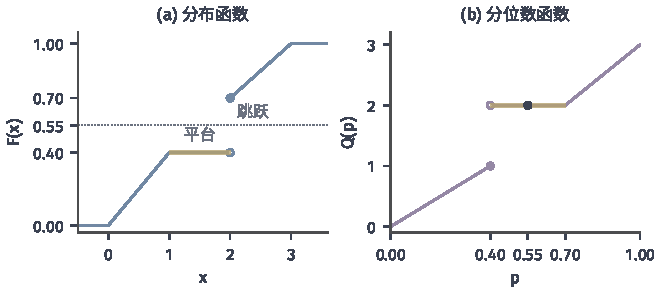
\includegraphics[width=112mm]{figures/01-basic-mathematics/05-probability-and-statistics-basics/matplotlib/prob-quantile-inverse/figure.pdf}
  \caption{分位数作为分布函数的广义逆。(a)分布函数在$[1,2)$上有平台（黄色），在$x=2$处从$0.4$跳到$0.7$；(b)相应的分位数函数$Q(p)=\inf\{x:F(x)\geq p\}$在$p=0.4$处从$1$跳到$2$，在$(0.4,0.7]$上保持为$2$（黄色）。点线$p=0.55$与(a)的曲线没有交点，(b)中黑点给出$Q(0.55)=2$。}
  \label{fig:prob-quantile-inverse}
\end{figure}

\begin{example}[几个分位数]
\label{ex:prob-quantile-examples}
例~\ref{ex:prob-three-cdfs}(b)中$F_T(t)=1-e^{-t}$连续严格递增，解$1-e^{-t}=p$得$Q(p)=-\ln(1-p)$。中位数是$\ln2\approx0.693$分钟，$0.9$分位数是$\ln10\approx2.303$分钟：九成顾客的等待不超过约$2.3$分钟。公平骰子的点数满足$F(3)=1/2$，所以中位数是$\inf\{x:F(x)\geq1/2\}=3$；尽管$[3,4)$上都有$F(x)=1/2$，约定取最小者$3$。
\end{example}

\paragraph{位置的不同度量}
均值、中位数和其他分位数都描述分布的“位置”，但回答的问题不同。中位数只依赖取值的顺序：它把概率分成各一半，与最大的那些值到底有多大无关。均值则按取值大小加权，远处的取值即使概率很小，也会把均值拉过去。分位数还可以描述其他位置，例如$0.9$分位数刻画右尾的典型界限，两个四分位数之差$Q(3/4)-Q(1/4)$则从另一个角度衡量离散程度。

若分布关于某点$c$对称且期望存在，则均值等于$c$，而$c$左右两侧的概率也各为一半，此时均值与中位数描述同一个中心；偏斜分布中二者通常不同。再引入\term{众数}（mode），即质量函数或密度函数取最大值的位置，它表示取值最集中的地方。

\begin{example}[右偏分布的三种位置]
\label{ex:prob-skewed-locations}
设$X$的密度为$f(x)=xe^{-x}$（$x>0$）。分部积分得$\int_0^\infty xe^{-x}\,\mathrm{d}x=1$，确为密度；均值$\mathbb{E}[X]=\int_0^\infty x^2e^{-x}\,\mathrm{d}x=2$。由$f'(x)=(1-x)e^{-x}$，众数为$1$。分布函数是$F(x)=1-(1+x)e^{-x}$，中位数$m$满足$(1+m)e^{-m}=1/2$，数值求解得$m\approx1.678$。三者满足众数$<$中位数$<$均值，如图~\ref{fig:prob-skewed-locations}所示：右侧的长尾把均值拉向右边，中位数受影响较小，众数只看密度峰的位置。
\end{example}

\begin{figure}[htbp]
  \centering
  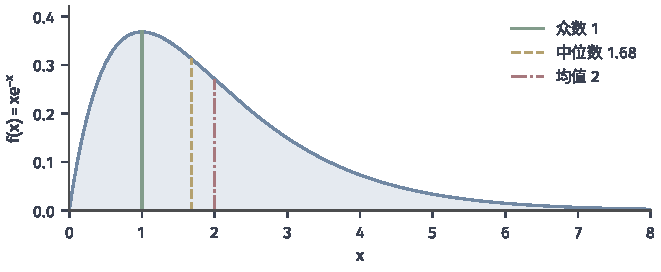
\includegraphics[width=112mm]{figures/01-basic-mathematics/05-probability-and-statistics-basics/matplotlib/prob-skewed-locations/figure.pdf}
  \caption{右偏密度$f(x)=xe^{-x}$（$x>0$）的三种位置。众数$1$是密度峰的位置，中位数约$1.68$把阴影面积分成相等的两半，均值$2$受右侧长尾影响最大。在这个右偏分布中，三者按众数、中位数、均值的顺序从左到右排列。}
  \label{fig:prob-skewed-locations}
\end{figure}

均值与中位数的差别在报告中很常见。收入、等待时间这类右偏变量，少数很大的取值会使均值明显高于中位数，此时“平均收入”与“典型收入”说的不是同一件事。选择哪种位置，取决于问题关心总量（均值乘以人数就是总量）还是典型个体（中位数）。

\subsection{矩、偏度与峰度}
\label{sec:prob-moments}

\paragraph{原点矩与中心矩}
均值与方差分别是$X$与$(X-\mu)^2$的期望。把幂次推广到一般正整数$k$，就得到一族数值特征，统称为矩。

\begin{definition}[矩]
\label{def:prob-moments}
设$k$为正整数且$\mathbb{E}\bigl[|X|^k\bigr]<\infty$。称$\mathbb{E}[X^k]$为$X$的$k$阶\term{原点矩}（raw moment），称$\mathbb{E}\bigl[(X-\mu)^k\bigr]$为$k$阶\term{中心矩}（central moment），其中$\mu=\mathbb{E}[X]$。
\end{definition}

在这个体系中，均值是一阶原点矩，方差是二阶中心矩；一阶中心矩恒为零。高阶矩有限是比低阶矩有限更强的要求：若$j<k$，由$|x|^j\leq1+|x|^k$，$k$阶矩有限蕴含$j$阶矩有限。中心矩可以用原点矩展开计算，例如$\mathbb{E}[(X-\mu)^3]=\mathbb{E}[X^3]-3\mu\,\mathbb{E}[X^2]+2\mu^3$。

尾部衰减的速度决定了哪些矩存在。设$X$的密度为$f(x)=3x^{-4}$（$x\geq1$）。则$\mathbb{E}[X]=\int_1^\infty3x^{-3}\,\mathrm{d}x=\frac32$，$\mathbb{E}[X^2]=\int_1^\infty3x^{-2}\,\mathrm{d}x=3$，方差为$3-\frac94=\frac34$；但$\mathbb{E}[X^3]=\int_1^\infty3x^{-1}\,\mathrm{d}x=+\infty$。这个分布有有限的均值和方差，三阶以上的矩都不存在。

\paragraph{偏度与峰度}
三阶、四阶中心矩记录了分布形状的信息，但它们随单位变化：把$X$乘以$a$，三阶中心矩乘以$a^3$。用标准差的相应次幂相除，就得到与单位无关的形状指标。

\begin{definition}[偏度与峰度]
\label{def:prob-skewness-kurtosis}
设$\operatorname{Var}(X)=\sigma^2>0$。若三阶矩有限，称$\gamma_1=\mathbb{E}\bigl[(X-\mu)^3\bigr]/\sigma^3$为$X$的\term{偏度}（skewness）；若四阶矩有限，称$\kappa=\mathbb{E}\bigl[(X-\mu)^4\bigr]/\sigma^4$为$X$的\term{峰度}（kurtosis）。
\end{definition}

偏度衡量不对称性：立方保留了偏差的符号，右侧远处的大偏差使偏度为正，左侧的使之为负；对称分布的偏度为零。峰度以四次方放大远离均值的偏差，主要反映尾部的厚重程度，而不是峰顶的尖锐。第~\ref{sec:prob-gaussian}节的高斯分布峰度为$3$，因此$\kappa-3$常称为超额峰度，用来与高斯尾部比较。

\begin{example}[等待时间的偏度与峰度]
\label{ex:prob-exponential-shape}
对密度$f(t)=e^{-t}$（$t\geq0$），分部积分递推给出$\int_0^\infty t^ke^{-t}\,\mathrm{d}t=k!$，即$\mathbb{E}[T^k]=k!$。于是$\mu=1$，$\sigma^2=2-1=1$，
\[
  \begin{aligned}
  \mathbb{E}[(T-1)^3]&=6-3\cdot2+3\cdot1-1=2,\\
  \mathbb{E}[(T-1)^4]&=24-4\cdot6+6\cdot2-4\cdot1+1=9 .
  \end{aligned}
\]
偏度为$2$，峰度为$9$：分布明显右偏，尾部比高斯分布厚得多。
\end{example}

有限个数值特征一般不能确定整个分布。以各$1/2$的概率取$\pm1$的变量与区间$(-\sqrt3,\sqrt3)$上的均匀分布，均值都是$0$、方差都是$1$、偏度都是$0$，前者只取两个值，后者却连续分布。即使所有阶的矩都存在且对应相等，两个分布也可能不同：第~\ref{sec:prob-density-change}节的对数正态分布就是经典例子，存在另一个分布与它的各阶矩全部相同。所以数值特征是对分布的概括，而不是替代；需要完整分布时，仍要回到分布函数、质量函数或密度。

\section{常见离散分布}
\label{sec:prob-discrete-models}

很多随机现象的分布可以由少数假设推出，并由一两个参数完全确定。本节按随机结果的含义组织离散模型：一次二元结果（Bernoulli分布）、一次类别选择（类别分布）、固定次数内的成功数（二项分布）、首次成功所需的次数（几何分布），以及没有固定上限的事件计数（Poisson分布）。每个模型都要说明它从什么假设得来，假设改变时为何不能沿用。图~\ref{fig:prob-discrete-pmfs}先给出后四类分布质量函数的样子。

\begin{figure*}[htbp]
  \centering
  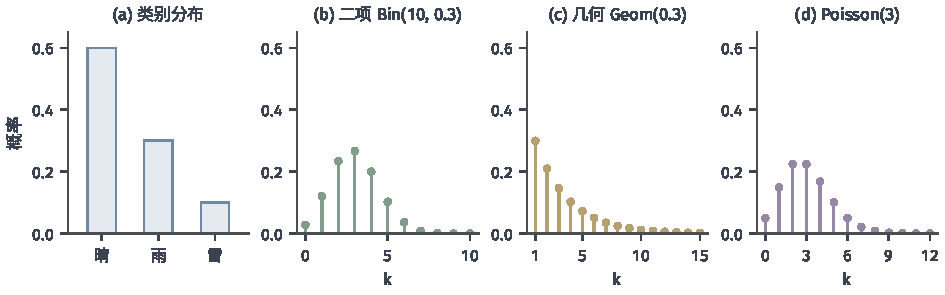
\includegraphics[width=160mm]{figures/01-basic-mathematics/05-probability-and-statistics-basics/matplotlib/prob-discrete-pmfs/figure.pdf}
  \caption{常见离散分布的质量函数。(a)三个天气类别的类别分布，概率依次为$0.6,0.3,0.1$，横轴只是类别标签；(b)$10$次独立试验、成功概率$0.3$的成功次数，集中在均值$3$附近；(c)成功概率$0.3$时首次成功所需的试验次数，从$1$开始按公比$0.7$递减；(d)均值为$3$的Poisson计数，取值没有上限，图中只画到$12$。}
  \label{fig:prob-discrete-pmfs}
\end{figure*}

\subsection{Bernoulli分布}
\label{sec:prob-bernoulli}

\paragraph{一次二元结果}
抽检一件产品是否为次品、一次点击是否发生、一枚硬币是否正面，都只有两种结果。把“成功”记为$1$、“失败”记为$0$，得到只取两个值的随机变量，它的分布只需一个参数。

\begin{definition}[Bernoulli分布]
\label{def:prob-bernoulli}
设$0\leq p\leq1$。若$\mathbb{P}(X=1)=p$，$\mathbb{P}(X=0)=1-p$，就称$X$服从参数为$p$的\term{Bernoulli分布}（Bernoulli distribution），记作$X\sim\operatorname{Bernoulli}(p)$。其质量函数可以统一写成
\[
  p_X(x)=p^x(1-p)^{1-x},\qquad x\in\{0,1\},
\]
其中约定$0^0=1$。
\end{definition}

直接计算$\mathbb{E}[X]=0\cdot(1-p)+1\cdot p=p$。由于$X$只取$0$和$1$，$X^2=X$，所以$\mathbb{E}[X^2]=p$，
\[
  \operatorname{Var}(X)=p-p^2=p(1-p).
\]
方差在$p=1/2$时最大，为$1/4$；$p$接近$0$或$1$时结果几乎确定，方差趋于零。

\paragraph{指示变量与事件概率}
任何事件$A$都对应一个Bernoulli变量，即它的指示变量$\mathbb{I}_A$，其参数就是$\mathbb{P}(A)$。于是
\[
  \mathbb{E}[\mathbb{I}_A]=\mathbb{P}(A).
\]
这个等式把概率写成了期望，从而可以借助期望的线性性计算“发生了几个事件”。设$A_1,\dots,A_n$为事件，$N=\mathbb{I}_{A_1}+\dots+\mathbb{I}_{A_n}$就是其中发生的个数，它的均值是$\mathbb{E}[N]=\sum_i\mathbb{P}(A_i)$。这里用到的是多个指示变量之和的线性性：$N$在每个样本点上都是各指示函数值之和，按样本点求概率加权和时可以逐项拆开（样本空间可数时这就是求和的线性性，一般情形见第~\ref{sec:rvec-moments}节）。这一步不需要任何独立性。

\begin{example}[抽检样本中次品个数的均值]
\label{ex:prob-inspection-mean}
回到例~\ref{ex:prob-inspection-hypergeometric}，从$5$件次品、$95$件合格品中不放回抽取$10$件。若按顺序抽取，第$i$件是哪一件产品，由对称性对$100$件产品等可能，所以“第$i$件是次品”的概率为$5/100$。样本中次品个数为$N=\sum_{i=1}^{10}\mathbb{I}_{A_i}$，其中$A_i$为“第$i$件是次品”，于是$\mathbb{E}[N]=10\times0.05=0.5$。各次抽取并不独立，但这不影响均值的计算。
\end{example}

同样，若$n$次试验中成功的指示变量为$X_1,\dots,X_n$，成功的比例$\frac1n\sum_iX_i$的均值等于各次成功概率的平均。频数、计数和样本比例都可以这样写成指示变量之和，后面各章会反复使用这一表示。

\subsection{类别分布}
\label{sec:prob-categorical}

\paragraph{有限个类别}
天气可以是晴、雨、雪，一张图片可以属于$K$个类别之一。把二元结果推广到有限个类别，就要为每个类别指定一个概率。

\begin{definition}[类别分布]
\label{def:prob-categorical}
设$\bm{\pi}=(\pi_1,\dots,\pi_K)^{\top}$满足$\pi_k\geq0$且$\sum_{k=1}^K\pi_k=1$。若随机变量$C$取值于$\{1,\dots,K\}$，且$\mathbb{P}(C=k)=\pi_k$，就称$C$服从\term{类别分布}（categorical distribution），记作$C\sim\operatorname{Cat}(\bm{\pi})$。
\end{definition}

满足上述条件的向量$\bm{\pi}$称为概率向量。$K=2$时，类别分布就是Bernoulli分布换了一种编号；公平骰子的点数是$K=6$、$\pi_k=1/6$的类别分布。图~\ref{fig:prob-discrete-pmfs}(a)画的是$\bm{\pi}=(0.6,0.3,0.1)^{\top}$的天气分布。

\paragraph{标签不是数量}
类别分布用$1,\dots,K$作编号，但这些数字只是标签，没有大小意义。若把晴、雨、雪编为$1,2,3$，“编号的均值”是$1\times0.6+2\times0.3+3\times0.1=1.5$；改为雪、雨、晴依次编$1,2,3$，同一个分布的“编号均值”就变成$3\times0.6+2\times0.3+1\times0.1=2.5$。结果随任意的编号方式而变，并不表示“平均天气介于晴和雨之间”。骰子点数是例外，因为点数本身就是数量。

需要对类别作数值计算时，常用独热编码（one-hot encoding）：把类别$C=k$表示成第$k$个分量为$1$、其余为$0$的向量$\bm{e}_C\in\mathbb{R}^K$。$\bm{e}_C$的第$k$个分量正是指示变量$\mathbb{I}_{\{C=k\}}$，其期望为$\pi_k$，所以$\bm{e}_C$的逐分量期望就是概率向量$\bm{\pi}$。这一表示不依赖编号顺序，向量值随机变量的系统讨论见第~\ref{chap:random-vectors}章。

\subsection{二项分布}
\label{sec:prob-binomial}

\paragraph{固定次数中的成功数}
把一次Bernoulli试验独立地重复$n$次，成功总次数是多少？例如有放回地抽检$10$件产品，每件是次品的概率为$0.05$，样本中的次品数就是这样的计数。设$X_1,\dots,X_n$为各次试验的成功指示，满足三个条件：试验次数$n$事先固定；每次成功概率都是$p$；各次试验相互独立，即事件$\{X_i=1\}$（$i=1,\dots,n$）相互独立。令$S=X_1+\dots+X_n$。

考虑$S=k$。任意一个指定位置有$k$次成功、$n-k$次失败的结果序列，由相互独立性，其概率是$p^k(1-p)^{n-k}$，与成功出现在哪些位置无关。从$n$个位置中选出$k$个成功位置共有$\binom nk$种方式（第~\ref{chap:counting}章），这些序列两两互斥，因此
\[
  \mathbb{P}(S=k)=\binom{n}{k}p^k(1-p)^{n-k},\qquad k=0,1,\dots,n .
\]

\begin{definition}[二项分布]
\label{def:prob-binomial}
具有上述质量函数的分布称为参数为$n,p$的\term{二项分布}（binomial distribution），记作$S\sim\operatorname{Bin}(n,p)$。
\end{definition}

由二项式定理，$\sum_{k=0}^n\binom nkp^k(1-p)^{n-k}=(p+1-p)^n=1$，质量函数确实归一。$n=1$时它就是$\operatorname{Bernoulli}(p)$。

\paragraph{均值与方差}
均值可以用指示变量之和直接得到：$\mathbb{E}[S]=\sum_i\mathbb{E}[X_i]=np$。方差要计算$\mathbb{E}[S^2]$，这里从质量函数出发。利用组合恒等式$k\binom nk=n\binom{n-1}{k-1}$及其推论$k(k-1)\binom nk=n(n-1)\binom{n-2}{k-2}$，
\[
  \begin{aligned}
  \mathbb{E}[S(S-1)]&=\sum_{k=2}^nn(n-1)\binom{n-2}{k-2}p^k(1-p)^{n-k}\\
  &=n(n-1)p^2\sum_{j=0}^{n-2}\binom{n-2}{j}p^j(1-p)^{n-2-j}=n(n-1)p^2,
  \end{aligned}
\]
最后一个和是$\operatorname{Bin}(n-2,p)$的总概率$1$。于是
\[
  \begin{aligned}
  \operatorname{Var}(S)&=\mathbb{E}[S(S-1)]+\mathbb{E}[S]-(\mathbb{E}[S])^2\\
  &=n(n-1)p^2+np-n^2p^2=np(1-p).
  \end{aligned}
\]
方差恰为$n$个Bernoulli方差之和；第~\ref{sec:rvec-moments}节会说明，这是独立变量的方差可以相加的一个特例。

\begin{example}[有放回抽检]
\label{ex:prob-inspection-binomial}
有放回地从次品率为$5\%$的产品中抽检$10$件，次品数$S\sim\operatorname{Bin}(10,0.05)$。样本中没有次品的概率是$0.95^{10}\approx0.5987$，均值为$0.5$，方差为$10\times0.05\times0.95=0.475$。
\end{example}

\paragraph{条件改变时}
二项模型的三个条件缺一不可。例~\ref{ex:prob-inspection-hypergeometric}是不放回抽检，每抽走一件，剩余产品的构成就变了，各次抽取不独立，样本中没有次品的概率是$0.5838$而不是$0.5987$。由于样本只占总体的$10\%$，两者相差不大；样本占总体比例越大，差别越明显。不放回抽样下次品数的精确分布称为超几何分布，其均值仍为$0.5$（例~\ref{ex:prob-inspection-mean}），方差则不同。

成功概率不相同时同样不能使用二项分布。设两次试验相互独立，第一次必然失败（$p_1=0$），第二次必然成功（$p_2=1$）。成功总数恒为$1$，方差为$0$；而平均成功概率为$1/2$的$\operatorname{Bin}(2,1/2)$方差为$1/2$。均值相同，波动却完全不同，原因是各次试验的概率并不一致。

\subsection{几何分布}
\label{sec:prob-geometric}

\paragraph{首次成功所需的次数}
反复掷骰子，直到第一次出现$6$点为止，要掷多少次？二项分布固定次数、数成功个数；这里反过来，次数本身是随机的。设各次试验相互独立、成功概率都是$p\in(0,1]$，令$T$为首次成功时已进行的试验次数。

$T=k$意味着前$k-1$次都失败、第$k$次成功，由独立性
\[
  \mathbb{P}(T=k)=(1-p)^{k-1}p,\qquad k=1,2,\dots
\]

\begin{definition}[几何分布]
\label{def:prob-geometric}
具有上述质量函数的分布称为参数为$p$的\term{几何分布}（geometric distribution），记作$T\sim\operatorname{Geom}(p)$。
\end{definition}

由几何级数，$\sum_{k\geq1}(1-p)^{k-1}p=p\cdot\frac{1}{1-(1-p)}=1$。“首次成功晚于第$k$次”等价于“前$k$次全部失败”，所以尾概率有简洁的形式
\[
  \mathbb{P}(T>k)=(1-p)^k,\qquad k=0,1,2,\dots
\]
掷骰子等待$6$点时$p=1/6$，掷了$6$次还没出现$6$点的概率是$(5/6)^6\approx0.335$，并不算小。

\paragraph{均值与方差}
对取非负整数值的变量，期望可以用尾概率求和：
\[
  \begin{aligned}
  \mathbb{E}[T]&=\sum_{k\geq1}k\,\mathbb{P}(T=k)=\sum_{k\geq1}\sum_{j=1}^{k}\mathbb{P}(T=k)\\
  &=\sum_{j\geq1}\sum_{k\geq j}\mathbb{P}(T=k)=\sum_{j\geq0}\mathbb{P}(T>j).
  \end{aligned}
\]
第三步交换了两个求和的次序，各项非负，交换不改变结果。代入尾概率得$\mathbb{E}[T]=\sum_{j\geq0}(1-p)^j=1/p$：成功概率为$1/6$时平均要掷$6$次。方差需要$\mathbb{E}[T(T-1)]$。记$q=1-p$，对几何级数$\sum_{k\geq0}q^k=\frac{1}{1-q}$在$|q|<1$内逐项求导两次（幂级数在收敛区间内可以逐项求导，见第~\ref{sec:ru-termwise-differentiation}节），得$\sum_{k\geq2}k(k-1)q^{k-2}=\frac{2}{(1-q)^3}$，于是
\[
  \begin{aligned}
  \mathbb{E}[T(T-1)]&=pq\sum_{k\geq2}k(k-1)q^{k-2}=\frac{2pq}{p^3}=\frac{2(1-p)}{p^2},\\
  \operatorname{Var}(T)&=\frac{2(1-p)}{p^2}+\frac1p-\frac1{p^2}=\frac{1-p}{p^2}.
  \end{aligned}
\]

\paragraph{无记忆性与计数约定}
已经连续失败了$m$次，还要再等多久？用条件概率计算：
\[
  \mathbb{P}(T>m+k\mid T>m)=\frac{\mathbb{P}(T>m+k)}{\mathbb{P}(T>m)}=\frac{(1-p)^{m+k}}{(1-p)^m}=(1-p)^k,
\]
它恰好等于$\mathbb{P}(T>k)$。这里用到$\{T>m+k\}\subseteq\{T>m\}$，所以交集就是$\{T>m+k\}$。结论称为\term{无记忆性}（memorylessness）：已经失败了多少次，不影响剩余等待次数的分布。这符合独立试验的设定，因为过去的失败不会让下一次更容易成功。“已经很久没出$6$点了，下一次该出了”的想法，在独立试验下并不成立。

文献中还有另一种约定：记录首次成功之前的失败次数$N=T-1$，取值于$\{0,1,2,\dots\}$，质量函数为$(1-p)^kp$。两者只相差一个平移，$\mathbb{E}[N]=\frac{1-p}{p}$比$\mathbb{E}[T]$小$1$，方差相同。使用几何分布的公式前，要先确认采用的是哪种计数。

\subsection{Poisson分布}
\label{sec:prob-poisson}

\paragraph{固定范围内的事件计数}
一小时内到达客服中心的电话数、一页书上的印刷错误数、一个像素在曝光时间内接收的光子数，都是在固定的时间、空间范围内对事件计数。与二项分布不同，这类计数没有预先固定的试验次数，原则上可以取任意非负整数。

\begin{definition}[Poisson分布]
\label{def:prob-poisson}
设$\lambda>0$。若$N$取非负整数值，且
\[
  \mathbb{P}(N=k)=e^{-\lambda}\frac{\lambda^k}{k!},\qquad k=0,1,2,\dots,
\]
就称$N$服从参数为$\lambda$的\term{Poisson分布}（Poisson distribution），记作$N\sim\operatorname{Poisson}(\lambda)$。
\end{definition}

由指数函数的幂级数$e^{\lambda}=\sum_{k\geq0}\lambda^k/k!$，质量函数之和为$1$。均值为
\[
  \mathbb{E}[N]=\sum_{k\geq1}k\,e^{-\lambda}\frac{\lambda^k}{k!}=\lambda e^{-\lambda}\sum_{k\geq1}\frac{\lambda^{k-1}}{(k-1)!}=\lambda .
\]
同样地，$\mathbb{E}[N(N-1)]=\lambda^2e^{-\lambda}\sum_{k\geq2}\frac{\lambda^{k-2}}{(k-2)!}=\lambda^2$，所以$\operatorname{Var}(N)=\lambda^2+\lambda-\lambda^2=\lambda$。参数$\lambda$同时是均值和方差。

\begin{example}[客服电话]
\label{ex:prob-poisson-calls}
设每小时来电数$N\sim\operatorname{Poisson}(3)$。一小时内没有来电的概率是$e^{-3}\approx0.0498$。来电不少于$5$个的概率为
\[
  1-e^{-3}\Bigl(1+3+\frac{9}{2}+\frac{27}{6}+\frac{81}{24}\Bigr)=1-16.375\,e^{-3}\approx0.185 .
\]
\end{example}

\paragraph{稀有事件的二项极限}
Poisson模型可以看作大量独立小机会的累计。把一小时切成$n$个小时段，假设每段至多来一个电话、来电概率为$\lambda/n$，且各段相互独立，那么来电总数服从$\operatorname{Bin}(n,\lambda/n)$，均值固定为$\lambda$。时段切得越细，这个二项分布越接近$\operatorname{Poisson}(\lambda)$。

\begin{theorem}[二项分布的Poisson极限]
\label{thm:prob-binomial-poisson-limit}
设$\lambda>0$，$p_n=\lambda/n$。对每个固定的非负整数$k$，
\[
  \lim_{n\to\infty}\binom{n}{k}p_n^k(1-p_n)^{n-k}=e^{-\lambda}\frac{\lambda^k}{k!}.
\]
\end{theorem}
\begin{proof}
把质量函数拆成三个因子：
\[
  \binom nk\Bigl(\frac\lambda n\Bigr)^k\Bigl(1-\frac\lambda n\Bigr)^{n-k}
  =\frac{\lambda^k}{k!}\cdot\frac{n(n-1)\cdots(n-k+1)}{n^k}\cdot\Bigl(1-\frac\lambda n\Bigr)^{n}\Bigl(1-\frac\lambda n\Bigr)^{-k}.
\]
$k$固定时，第二个因子是$k$个分别趋于$1$的因子$\frac{n-j}{n}$之积，极限为$1$；$(1-\lambda/n)^{-k}\to1$；而取对数后$n\ln(1-\lambda/n)\to-\lambda$，由指数函数的连续性$(1-\lambda/n)^n\to e^{-\lambda}$，这与第~\ref{chap:univariate-differentiation}章处理$(1+1/n)^n\to e$的方法相同。三者相乘即得结论。
\end{proof}

图~\ref{fig:prob-binomial-poisson}比较了$\operatorname{Bin}(n,3/n)$与$\operatorname{Poisson}(3)$。$n=6$时二项分布明显更集中于均值附近，因为它最多只能取到$6$；$n=60$时两者在图上几乎重合。这也说明了两个模型的差别：二项计数有已知的上限$n$，方差$np(1-p)$小于均值；Poisson计数没有上限，方差等于均值。只因均值接近就混用两个模型是不对的，要看计数是否有固定的试验次数，以及每次机会是否稀少。

\begin{figure}[htbp]
  \centering
  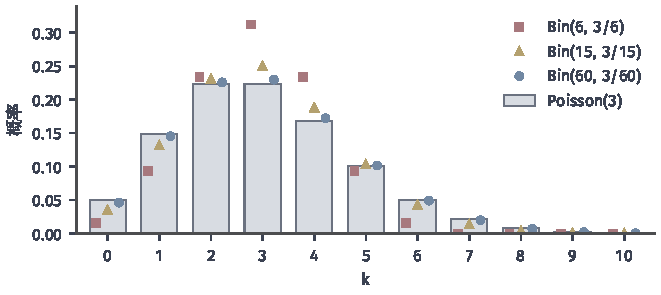
\includegraphics[width=112mm]{figures/01-basic-mathematics/05-probability-and-statistics-basics/matplotlib/prob-binomial-poisson/figure.pdf}
  \caption{稀有事件下二项分布逼近Poisson分布。灰色柱为$\operatorname{Poisson}(3)$的质量函数，三种标记分别为$n=6,15,60$、成功概率$3/n$的二项分布，均值都为$3$。$n$越大，二项分布越接近灰色柱；$n=6$时二项分布在$k=3$处偏高，并且不能取大于$6$的值。}
  \label{fig:prob-binomial-poisson}
\end{figure}

定理只说明了一种来源：满足“机会很多、每次很稀少、彼此独立”时，Poisson模型是合理的近似。仅知道计数非负并不足以采用Poisson分布；例如若来电成批出现，方差会明显大于均值。不同时间段的计数之间怎样联系、到达时刻怎样分布，需要Poisson过程来描述，可参考\BookChapterRef{chap:random-sequences-and-processes}{卷3《数学准备：优化、动力系统与信号处理》的“随机序列与随机过程”章}。

\section{常见连续分布}
\label{sec:prob-continuous-models}

连续模型同样从取值范围和形状假设出发。本节依次研究：有界区间上不偏向任何位置的取值（均匀分布），非负的等待时间（指数分布），围绕中心对称波动的量（高斯分布），以及更一般的正值变量与比例（Gamma分布与Beta分布）。图~\ref{fig:prob-continuous-densities}汇总了后四类分布在不同参数下的密度。

\begin{figure*}[htbp]
  \centering
  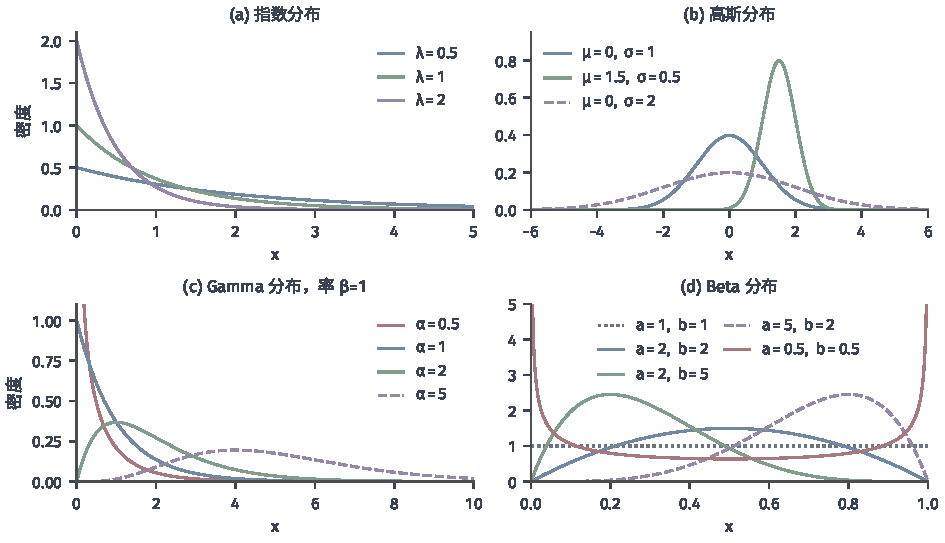
\includegraphics[width=160mm]{figures/01-basic-mathematics/05-probability-and-statistics-basics/matplotlib/prob-continuous-densities/figure.pdf}
  \caption{常见连续分布的密度。(a)指数分布，率$\lambda$越大，密度在$0$处越高、衰减越快；(b)高斯分布，$\mu$决定中心，$\sigma$决定宽度，$\sigma$减半时峰高加倍；(c)率为$1$的Gamma分布，形状$\alpha<1$时密度在$0$附近无界（图中截断），$\alpha=1$即指数分布，$\alpha>1$时出现单峰；(d)Beta分布，$a=b=1$为均匀分布，$a=b>1$关于$1/2$对称，$a<b$时偏向$0$、$a>b$时偏向$1$，$a=b=0.5$时呈U形（图中截断）。}
  \label{fig:prob-continuous-densities}
\end{figure*}

\subsection{均匀分布}
\label{sec:prob-uniform}

\paragraph{等长区间等概率}
把一根长为$1$米的绳子随机剪断，若没有理由认为任何位置更容易被剪中，自然要求长度相同的两段区间被剪中的概率相同。这一要求决定了密度在区间内必须是常数。

\begin{definition}[均匀分布]
\label{def:prob-uniform}
设$a<b$。若$X$的密度为
\[
  f_X(x)=\frac{1}{b-a},\qquad a<x<b,
\]
在区间外为$0$，就称$X$服从区间$(a,b)$上的\term{均匀分布}（uniform distribution），记作$X\sim\operatorname{U}(a,b)$。
\end{definition}

对$a\leq x\leq b$，分布函数为$F_X(x)=\frac{x-a}{b-a}$，在$x<a$时为$0$、$x>b$时为$1$。由对称性或直接积分，$\mathbb{E}[X]=\frac{a+b}{2}$。再由$\mathbb{E}[X^2]=\frac{1}{b-a}\int_a^bx^2\,\mathrm{d}x=\frac{a^2+ab+b^2}{3}$，
\[
  \operatorname{Var}(X)=\frac{a^2+ab+b^2}{3}-\frac{(a+b)^2}{4}=\frac{(b-a)^2}{12}.
\]
标准差$\frac{b-a}{2\sqrt3}\approx0.29(b-a)$与区间长度成正比，与区间位置无关。

\paragraph{均匀的含义与用途}
区间内密度相同，意思是任何子区间的概率只取决于它的长度：$\mathbb{P}(c<X\leq d)=\frac{d-c}{b-a}$，与子区间在哪里无关。这是一个关于对称性的模型假设，并不等于“对结果一无所知”。例如对一个正数比例$R$，若假设$R$在$(0,1)$上均匀，那么$R^2$就不再均匀（第~\ref{sec:prob-cdf-method}节的方法可以算出它的分布）；对同一未知量的不同表示，“均匀”给出不同的结论。

标准均匀变量$U\sim\operatorname{U}(0,1)$是随机模拟的基础。计算机的随机数生成器产生近似服从$\operatorname{U}(0,1)$的数，其他分布的随机数则由它经过变换得到。第~\ref{sec:prob-cdf-method}节会给出第一个例子：$U$经过对数变换后服从指数分布；一般的构造留到第~\ref{sec:rvec-generation}节。

\subsection{指数分布}
\label{sec:prob-exponential}

\paragraph{等待时间模型}
例~\ref{ex:prob-three-cdfs}(b)的等待时间满足$\mathbb{P}(T>t)=e^{-t}$。允许不同的时间尺度，就得到一族非负等待时间模型，用率参数$\lambda$表示单位时间内事件发生的强度。

\begin{definition}[指数分布]
\label{def:prob-exponential}
设$\lambda>0$。若$T$的密度为
\[
  f_T(t)=\lambda e^{-\lambda t},\qquad t\geq0,
\]
在$t<0$时为$0$，就称$T$服从率为$\lambda$的\term{指数分布}（exponential distribution），记作$T\sim\operatorname{Exp}(\lambda)$。
\end{definition}

积分得分布函数$F_T(t)=1-e^{-\lambda t}$与尾概率$\mathbb{P}(T>t)=e^{-\lambda t}$（$t\geq0$）。换元$s=\lambda t$并利用$\int_0^\infty s^ke^{-s}\,\mathrm{d}s=k!$（例~\ref{ex:prob-exponential-shape}），得$\mathbb{E}[T^k]=k!/\lambda^k$，于是
\[
  \mathbb{E}[T]=\frac1\lambda,\qquad \operatorname{Var}(T)=\frac{2}{\lambda^2}-\frac1{\lambda^2}=\frac1{\lambda^2}.
\]
率$\lambda$越大，事件来得越快，平均等待$1/\lambda$越短。标准差与均值相等。

\begin{example}[窗口等待]
\label{ex:prob-exponential-wait}
设等待时间平均为$5$分钟，取$T\sim\operatorname{Exp}(0.2)$。等待超过$10$分钟的概率是$e^{-2}\approx0.135$。中位数$\frac{\ln2}{0.2}\approx3.47$分钟，小于均值$5$分钟，这与第~\ref{sec:prob-quantiles}节右偏分布的规律一致；$0.9$分位数为$5\ln10\approx11.5$分钟。
\end{example}

\paragraph{无记忆性}
指数分布与几何分布一样具有无记忆性：对$s,t\geq0$，
\[
  \mathbb{P}(T>s+t\mid T>s)=\frac{\mathbb{P}(T>s+t)}{\mathbb{P}(T>s)}=\frac{e^{-\lambda(s+t)}}{e^{-\lambda s}}=e^{-\lambda t}=\mathbb{P}(T>t).
\]
已经等了$s$分钟，剩余等待时间超过$t$的概率与刚开始等时完全相同。

这种相似并非巧合，指数分布可以看作几何分布的连续时间版本。把时间切成长度为$h$的小段，每段内事件发生的概率为$\lambda h$，各段独立，首次发生所在的段数$T_h\sim\operatorname{Geom}(\lambda h)$。对应的等待时间约为$hT_h$，其尾概率$\mathbb{P}(hT_h>t)=(1-\lambda h)^{\lfloor t/h\rfloor}$在$h\to0$时趋于$e^{-\lambda t}$。几何分布数的是离散的试验次数，指数分布量的是连续的时间长度，二者的无记忆性都来自“每一刻发生的机会不随已等待的时间改变”。

无记忆性不是所有等待时间都有的性质。若等待时间$T\sim\operatorname{U}(0,10)$，已知已等了$5$分钟，再等超过$2$分钟的概率是$\mathbb{P}(T>7\mid T>5)=\frac{3/10}{5/10}=0.6$，而一开始等待超过$2$分钟的概率是$0.8$：等得越久，剩余的等待越短。机械零件因磨损而老化，其寿命也不满足无记忆性。是否采用指数模型，要看“剩余等待与已等待时间无关”这一假设是否合理。

\subsection{高斯分布}
\label{sec:prob-gaussian}

\paragraph{标准高斯密度}
测量误差、身高、考试成绩这类量，常在一个中心值两侧对称波动，离中心越远越少见。描述这种形状最重要的模型是高斯分布，也称正态分布。我们先看中心在$0$、尺度为$1$的情形。

\begin{definition}[高斯分布]
\label{def:prob-gaussian}
密度
\[
  \varphi(z)=\frac{1}{\sqrt{2\pi}}e^{-z^2/2},\qquad z\in\mathbb{R}
\]
称为标准高斯密度，具有该密度的$Z$称为服从\term{标准正态分布}（standard normal distribution），记作$Z\sim\mathcal{N}(0,1)$。设$\mu\in\mathbb{R}$，$\sigma>0$，若$X$的密度为
\[
  f_X(x)=\frac{1}{\sqrt{2\pi}\,\sigma}\exp\Bigl(-\frac{(x-\mu)^2}{2\sigma^2}\Bigr)=\frac1\sigma\varphi\Bigl(\frac{x-\mu}{\sigma}\Bigr),
\]
就称$X$服从参数为$\mu,\sigma^2$的\term{高斯分布}（Gaussian distribution），也称\term{正态分布}（normal distribution），记作$X\sim\mathcal{N}(\mu,\sigma^2)$。
\end{definition}

$\varphi$的归一化依赖积分$\int_{-\infty}^{\infty}e^{-z^2/2}\,\mathrm{d}z=\sqrt{2\pi}$。$e^{-z^2/2}$没有初等原函数，这个积分值通常借助二重积分的极坐标换元求得（第~\ref{chap:multivariate-integration}章）。$\varphi$是偶函数，且尾部比任何多项式衰减得都快，所以各阶矩都有限，奇函数$z\varphi(z)$的积分为零，$\mathbb{E}[Z]=0$。方差由分部积分得到：利用$\varphi'(z)=-z\varphi(z)$，
\[
  \mathbb{E}[Z^2]=\int_{-\infty}^{\infty}z\cdot z\varphi(z)\,\mathrm{d}z=\Bigl[-z\varphi(z)\Bigr]_{-\infty}^{\infty}+\int_{-\infty}^{\infty}\varphi(z)\,\mathrm{d}z=1 .
\]
所以$\operatorname{Var}(Z)=1$。同样分部积分一次可得$\mathbb{E}[Z^4]=3\,\mathbb{E}[Z^2]=3$，这就是第~\ref{sec:prob-moments}节所说高斯分布的峰度为$3$。一般的$X\sim\mathcal{N}(\mu,\sigma^2)$由$Z$平移缩放而来（第~\ref{sec:prob-standardization}节），因此$\mathbb{E}[X]=\mu$，$\operatorname{Var}(X)=\sigma^2$：两个参数正好是均值与方差。图~\ref{fig:prob-continuous-densities}(b)显示，$\mu$平移曲线的中心，$\sigma$同时决定宽度与峰高，$\sigma$越小，曲线越窄越高，面积始终为$1$。

\paragraph{尾概率}
标准正态的分布函数记作$\Phi(z)=\int_{-\infty}^z\varphi(t)\,\mathrm{d}t$。它没有初等表达式，需要查表或用软件计算。对称性给出$\Phi(-z)=1-\Phi(z)$，常用的几个值是
\[
  \mathbb{P}(|Z|\leq1)\approx0.683,\qquad \mathbb{P}(|Z|\leq2)\approx0.954,\qquad \mathbb{P}(|Z|\leq3)\approx0.997 .
\]
偏离均值超过三个标准差的概率不到$0.3\%$。高斯尾部衰减得极快，对$z>0$有估计
\[
  \mathbb{P}(Z>z)=\int_z^\infty\varphi(t)\,\mathrm{d}t\leq\int_z^\infty\frac tz\varphi(t)\,\mathrm{d}t=\frac{\varphi(z)}{z},
\]
其中不等号用到积分区域内$t/z\geq1$，最后一步利用$t\varphi(t)$的原函数是$-\varphi(t)$。尾概率至少以$e^{-z^2/2}$的速度下降，比指数分布的$e^{-\lambda t}$快得多。

\paragraph{标准化计算与分位数}
对一般的$X\sim\mathcal{N}(\mu,\sigma^2)$，在概率积分中换元$z=(x-\mu)/\sigma$，$\mathrm{d}x=\sigma\,\mathrm{d}z$，得
\[
  \begin{aligned}
  \mathbb{P}(a<X\leq b)&=\int_a^b\frac1\sigma\varphi\Bigl(\frac{x-\mu}{\sigma}\Bigr)\mathrm{d}x=\int_{(a-\mu)/\sigma}^{(b-\mu)/\sigma}\varphi(z)\,\mathrm{d}z\\
  &=\Phi\Bigl(\frac{b-\mu}{\sigma}\Bigr)-\Phi\Bigl(\frac{a-\mu}{\sigma}\Bigr).
  \end{aligned}
\]
所以任何高斯分布的概率都可以化为标准正态的分布函数值，只需一张$\Phi$的表。反方向，记标准正态的$p$分位数为$z_p=\Phi^{-1}(p)$，则$\mathcal{N}(\mu,\sigma^2)$的$p$分位数是$\mu+\sigma z_p$。常用值有$z_{0.95}\approx1.645$、$z_{0.975}\approx1.960$、$z_{0.99}\approx2.326$；由对称性$z_{1-p}=-z_p$。

\begin{example}[零件长度]
\label{ex:prob-gaussian-parts}
某零件长度$X\sim\mathcal{N}(50,0.2^2)$，单位为毫米，合格范围为$[49.6,50.4]$。标准化后，合格概率为$\Phi(2)-\Phi(-2)\approx0.954$。若要找一个上限，使只有$1\%$的零件超过它，则取$0.99$分位数$50+0.2\times2.326\approx50.47$毫米。
\end{example}

高斯分布在应用中如此常见，一个重要原因是许多独立小误差之和近似服从高斯分布。这需要对“和”的分布作专门研究，具体条件和含义见第~\ref{sec:samp-clt}节的中心极限定理；仅凭“误差是对称的”并不能推出高斯形状。

\subsection{Gamma分布}
\label{sec:prob-gamma}

\paragraph{Gamma函数与归一化}
例~\ref{ex:prob-skewed-locations}的密度$xe^{-x}$与指数密度$e^{-x}$都具有$x^{\alpha-1}e^{-\beta x}$的形状。它们构成一族灵活的正值分布：幂函数因子控制$0$附近的行为，指数因子控制尾部。要使这个形状成为密度，需要计算它的积分，这就引出Gamma函数。

\begin{definition}[Gamma函数]
\label{def:prob-gamma-function}
对$\alpha>0$，定义\term{Gamma函数}（Gamma function）
\[
  \Gamma(\alpha)=\int_0^\infty t^{\alpha-1}e^{-t}\,\mathrm{d}t .
\]
\end{definition}

条件$\alpha>0$保证$t^{\alpha-1}$在$0$附近可积，$e^{-t}$保证无穷远处可积，两处的反常积分都收敛（第~\ref{sec:ru-improper-integrals}节）。分部积分给出递推
\[
  \Gamma(\alpha+1)=\Bigl[-t^{\alpha}e^{-t}\Bigr]_0^\infty+\alpha\int_0^\infty t^{\alpha-1}e^{-t}\,\mathrm{d}t=\alpha\,\Gamma(\alpha),
\]
又$\Gamma(1)=1$，所以对正整数$n$有$\Gamma(n)=(n-1)!$，Gamma函数把阶乘延伸到正实数。换元$t=z^2/2$还给出$\Gamma(1/2)=\sqrt{2}\int_0^\infty e^{-z^2/2}\,\mathrm{d}z=\sqrt\pi$。对$\beta>0$，再换元$t=\beta x$，
\[
  \int_0^\infty x^{\alpha-1}e^{-\beta x}\,\mathrm{d}x=\frac{\Gamma(\alpha)}{\beta^\alpha}.
\]

\begin{definition}[Gamma分布]
\label{def:prob-gamma}
设$\alpha>0$，$\beta>0$。若$X$的密度为
\[
  f_X(x)=\frac{\beta^\alpha}{\Gamma(\alpha)}x^{\alpha-1}e^{-\beta x},\qquad x>0,
\]
在$x\leq0$时为$0$，就称$X$服从形状参数为$\alpha$、率参数为$\beta$的\term{Gamma分布}（Gamma distribution），记作$X\sim\operatorname{Gamma}(\alpha,\beta)$。
\end{definition}

由上式，密度的积分为$1$。同一个积分公式直接给出各阶矩：
\[
  \mathbb{E}[X^k]=\frac{\beta^\alpha}{\Gamma(\alpha)}\int_0^\infty x^{\alpha+k-1}e^{-\beta x}\,\mathrm{d}x=\frac{\Gamma(\alpha+k)}{\Gamma(\alpha)\beta^k}.
\]
由递推，$\mathbb{E}[X]=\alpha/\beta$，$\mathbb{E}[X^2]=\alpha(\alpha+1)/\beta^2$，于是$\operatorname{Var}(X)=\alpha/\beta^2$。形状参数决定曲线的样子：$\alpha<1$时密度在$0$附近趋于无穷；$\alpha=1$时在$0$处取最大值；$\alpha>1$时密度从$0$升起再下降，由导数为零得众数$(\alpha-1)/\beta$。图~\ref{fig:prob-continuous-densities}(c)画出了这三种情形。

\paragraph{特例与参数化}
$\alpha=1$时密度为$\beta e^{-\beta x}$，所以$\operatorname{Exp}(\lambda)=\operatorname{Gamma}(1,\lambda)$；例~\ref{ex:prob-skewed-locations}的密度$xe^{-x}$就是$\operatorname{Gamma}(2,1)$，其均值$2$、众数$1$与前面的计算一致。第~\ref{sec:rvec-transforms}节将证明，$n$个相互独立的$\operatorname{Exp}(\lambda)$等待时间之和服从$\operatorname{Gamma}(n,\lambda)$，这给出了整数形状参数的含义：等到第$n$个事件发生所需的总时间。

Gamma分布有两种常见的参数化。本书使用率参数$\beta$，它的单位是“每单位时间”；另一种使用尺度参数$\vartheta=1/\beta$，密度写作$\frac{1}{\Gamma(\alpha)\vartheta^\alpha}x^{\alpha-1}e^{-x/\vartheta}$，均值为$\alpha\vartheta$。两种写法描述同一族分布，但同一组数字含义不同：把“$\operatorname{Gamma}(2,0.5)$”读作率参数，均值是$2/0.5=4$；读作尺度参数，均值是$2\times0.5=1$。查阅公式或调用软件时，必须先确认用的是哪一种。

\subsection{Beta分布}
\label{sec:prob-beta}

\paragraph{区间上的比例}
点击率、合格率、某种成分的比例都在$0$与$1$之间。均匀分布对这类量太死板，我们希望有一族在$(0,1)$上形状灵活的分布，能偏向$0$、偏向$1$或集中在中间。仿照Gamma分布，取$r^{a-1}(1-r)^{b-1}$的形状，两个幂次分别控制两端附近的行为。

\begin{definition}[Beta分布]
\label{def:prob-beta}
对$a>0$，$b>0$，记\term{Beta函数}（Beta function）
\[
  B(a,b)=\int_0^1r^{a-1}(1-r)^{b-1}\,\mathrm{d}r .
\]
若$R$的密度为
\[
  f_R(r)=\frac{1}{B(a,b)}r^{a-1}(1-r)^{b-1},\qquad 0<r<1,
\]
在区间外为$0$，就称$R$服从参数为$a,b$的\term{Beta分布}（Beta distribution），记作$R\sim\operatorname{Beta}(a,b)$。
\end{definition}

$a,b>0$保证两端的反常积分收敛。$a=b=1$时密度恒为$1$，就是$\operatorname{U}(0,1)$。$a=b>1$时密度关于$1/2$对称、中间高两端低；$a>b$时概率偏向$1$，$a<b$时偏向$0$；$a,b<1$时密度在两端趋于无穷，呈U形。见图~\ref{fig:prob-continuous-densities}(d)。

\paragraph{均值与方差}
矩的计算归结为Beta函数之比：$\mathbb{E}[R]=B(a+1,b)/B(a,b)$。为求这个比值，先注意$r^{a-1}(1-r)^{b-1}=r^{a}(1-r)^{b-1}+r^{a-1}(1-r)^{b}$（把$1=r+(1-r)$乘进去），积分得
\[
  B(a,b)=B(a+1,b)+B(a,b+1).
\]
另一方面，对$B(a+1,b)=\int_0^1r^a(1-r)^{b-1}\,\mathrm{d}r$分部积分，取$-\frac1b(1-r)^b$为$(1-r)^{b-1}$的原函数，边界项在两端为零，得$B(a+1,b)=\frac abB(a,b+1)$。把两式联立消去$B(a,b+1)$，
\[
  B(a+1,b)=\frac{a}{a+b}B(a,b),\qquad\text{从而}\qquad\mathbb{E}[R]=\frac{a}{a+b}.
\]
再用一次同样的递推，$\mathbb{E}[R^2]=\frac{B(a+2,b)}{B(a,b)}=\frac{a+1}{a+b+1}\cdot\frac{a}{a+b}$，于是
\[
  \operatorname{Var}(R)=\frac{a(a+1)}{(a+b)(a+b+1)}-\frac{a^2}{(a+b)^2}=\frac{ab}{(a+b)^2(a+b+1)}.
\]
均值只取决于$a$在$a+b$中的比例，而$a+b$越大方差越小，分布越集中。例如$\operatorname{Beta}(2,8)$与$\operatorname{Beta}(20,80)$的均值都是$0.2$，方差分别约为$0.0145$与$0.0016$。

\paragraph{用途与构造}
Beta分布常用来描述一个随机比例，或者表达对未知成功概率$p$的不确定性：$a$、$b$可以理解为“相当于事先见过的成功与失败次数”，$a+b$越大，对$p$的判断越确定。第~\ref{sec:est-bayes}节会用它作为二项模型中成功概率的先验分布。Beta函数还与Gamma函数有关系$B(a,b)=\Gamma(a)\Gamma(b)/\Gamma(a+b)$，它来自一个构造：两个相互独立、率相同的Gamma变量$U\sim\operatorname{Gamma}(a,1)$、$V\sim\operatorname{Gamma}(b,1)$，比例$U/(U+V)$服从$\operatorname{Beta}(a,b)$。证明需要二元变量的变换，留到第~\ref{sec:rvec-transforms}节。

\section{一元随机变量的变换}
\label{sec:prob-univariate-transforms}
\label{sec:rv-pushforward}

知道等待时间$T$的分布，费用$2T+5$元、等待时间的对数$\ln T$、误差的平方$\varepsilon^2$的分布是什么？本节研究$Y=g(X)$的分布怎样由$X$的分布和函数$g$确定。我们先用分布函数给出对任何分布都适用的方法，再在可微条件下推出密度的变换公式，最后专门讨论最常用的平移、缩放与标准化。

\subsection{利用分布函数计算变换}
\label{sec:prob-cdf-method}

\paragraph{回到原变量的事件}
$Y=g(X)$仍是定义在同一样本空间上的随机变量，对每个结果$\omega$，$Y(\omega)=g(X(\omega))$。要求$Y$的分布函数，就把事件$\{Y\leq y\}$翻译回$X$的取值范围：
\[
  F_Y(y)=\mathbb{P}(g(X)\leq y)=\mathbb{P}\bigl(X\in\{x:g(x)\leq y\}\bigr).
\]
一般地，对实数集的子集$B$，有$\mathbb{P}(Y\in B)=\mathbb{P}\bigl(X\in g^{-1}(B)\bigr)$，其中$g^{-1}(B)=\{x:g(x)\in B\}$是$B$的逆像。由此得到的$Y$的分布，也称为$X$的分布经$g$的\term{分布推前}（pushforward），记作$P_{g(X)}$或$g_{\#}P_X$，即$g_{\#}P_X(B)=P_X\bigl(g^{-1}(B)\bigr)$。

实际计算分两步。先确定$Y$可能取值的范围，即$g$在$X$可能取值上的像；在这个范围之外，分布函数直接是$0$或$1$。再对范围内的每个$y$，解出不等式$g(x)\leq y$对应的$x$的集合，用$X$的分布计算它的概率。

\begin{example}[由均匀变量得到指数变量]
\label{ex:prob-uniform-to-exponential}
设$U\sim\operatorname{U}(0,1)$，$\lambda>0$，令$Y=-\frac1\lambda\ln(1-U)$。$1-U$取值于$(0,1)$，其对数为负，所以$Y$取值于$(0,\infty)$，$y\leq0$时$F_Y(y)=0$。对$y>0$，由于$u\mapsto-\frac1\lambda\ln(1-u)$严格递增，
\[
  F_Y(y)=\mathbb{P}\Bigl(-\tfrac1\lambda\ln(1-U)\leq y\Bigr)=\mathbb{P}\bigl(U\leq1-e^{-\lambda y}\bigr)=1-e^{-\lambda y}.
\]
这正是$\operatorname{Exp}(\lambda)$的分布函数。这个例子说明了随机模拟中怎样把均匀随机数变成指数随机数：所用的函数恰是指数分布函数的反函数。
\end{example}

\paragraph{非单调变换}
单调函数把$\{g(x)\leq y\}$变成一个区间，计算很直接。非单调时，一个$y$值可能来自多个$x$值，逆像可能是几段区间的并。最典型的是平方：对$y\geq0$，
\[
  \{X^2\leq y\}=\{-\sqrt y\leq X\leq\sqrt y\},\qquad
  F_{X^2}(y)=F_X(\sqrt y)-F_X\bigl((-\sqrt y)^-\bigr),
\]
$y<0$时$F_{X^2}(y)=0$。左端点用左极限，是因为区间包含$-\sqrt y$。这个公式对任何分布都成立，不要求$X$有密度。

\begin{example}[离散变量的平方]
\label{ex:prob-discrete-square}
设$X$在$\{-1,0,1,2\}$上等可能取值。$Y=X^2$的可能取值为$0,1,4$。$Y=1$的逆像是$\{-1,1\}$两个点，所以
\[
  \mathbb{P}(Y=0)=\frac14,\qquad\mathbb{P}(Y=1)=\frac14+\frac14=\frac12,\qquad\mathbb{P}(Y=4)=\frac14 .
\]
平方把$-1$与$1$合并到同一个值，它们的概率相加。
\end{example}

图~\ref{fig:prob-square-transform}(a)画出$X\sim\operatorname{U}(-1,2)$时的情形。阈值$y=0.49<1$时，逆像是对称的区间$[-0.7,0.7]$，两侧都在$X$的取值范围内；阈值$y=2.25>1$时，$-\sqrt y=-1.5$已在取值范围之外，逆像只剩$[-1,1.5]$。于是对$0\leq y\leq1$有$F_Y(y)=\frac{2\sqrt y}{3}$，对$1\leq y\leq4$有$F_Y(y)=\frac{\sqrt y+1}{3}$。同一个函数$g$，在$Y$取值范围的不同部分，逆像的形状也可能不同。

\subsection{密度的变量替换}
\label{sec:prob-density-change}

\paragraph{单调变换的密度公式}
若$X$有密度，我们常希望直接写出$Y$的密度，而不是每次都先求分布函数。在$g$严格单调且可微的条件下，从分布函数出发就能得到一个通用公式。

\begin{theorem}[一元密度的变量替换]
\label{thm:prob-density-change}
设$X$有密度$f_X$，且$f_X$在开区间$I$外为零。设$g:I\to J$是从$I$到开区间$J$的连续可微双射，且在$I$上$g'(x)\neq0$，其反函数记为$h=g^{-1}:J\to I$。则$Y=g(X)$有密度
\[
  f_Y(y)=f_X\bigl(h(y)\bigr)\,\bigl|h'(y)\bigr|,\qquad y\in J,
\]
在$J$外为零。
\end{theorem}
\begin{proof}
$g'$在区间$I$上连续且不为零，所以$g'$不变号，$g$严格单调，$h$也连续可微，且$h'(y)=1/g'(h(y))$。设$g$递增，并记$J=(c,d)$、$I=(a',b')$（端点可以是无穷）。对$y\in J$，$g(X)\leq y$等价于$X\leq h(y)$，于是
\[
  F_Y(y)=\int_{a'}^{h(y)}f_X(x)\,\mathrm{d}x=\int_{c}^{y}f_X\bigl(h(s)\bigr)h'(s)\,\mathrm{d}s,
\]
第二步是换元$x=h(s)$（定理~\ref{thm:ru-substitution}，在反常积分上取极限即可）。这说明$Y$的分布函数是$f_X(h(s))h'(s)$的累计，而$h'>0$，所以它就是$Y$的密度。若$g$递减，则$g(X)\leq y$等价于$X\geq h(y)$，同样换元得$F_Y(y)=\int_c^yf_X(h(s))\,(-h'(s))\,\mathrm{d}s$，此时$-h'(s)=|h'(s)|$。

若$f_X$在$h(y)$处连续，也可以直接对$F_Y(y)=F_X(h(y))$（递增情形）求导：由链式法则，$F_Y'(y)=f_X(h(y))\,h'(y)$，结果相同。上面用换元写出积分，是为了不必假设$f_X$连续。
\end{proof}

绝对导数因子$|h'(y)|$补偿的是区间长度的伸缩。$X$落在$x$附近长为$\Delta x$的小区间内的概率约为$f_X(x)\Delta x$，这个小区间被$g$映到$y=g(x)$附近长为$\Delta y\approx|g'(x)|\Delta x$的小区间，概率不变，于是$f_Y(y)\Delta y\approx f_X(x)\Delta x$，即$f_Y(y)\approx f_X(x)/|g'(x)|=f_X(h(y))|h'(y)|$。$g$把区间拉长的地方，密度相应降低；压缩的地方，密度相应升高。只把$x=h(y)$代入$f_X$而遗漏这个因子，所得函数一般积分不为$1$。

\begin{example}[对数正态分布]
\label{ex:prob-lognormal}
设$X\sim\mathcal{N}(\mu,\sigma^2)$，$Y=e^X$。这里$I=\mathbb{R}$，$J=(0,\infty)$，$h(y)=\ln y$，$h'(y)=1/y$。由定理~\ref{thm:prob-density-change}，
\[
  f_Y(y)=\frac{1}{\sigma y}\varphi\Bigl(\frac{\ln y-\mu}{\sigma}\Bigr),\qquad y>0 .
\]
$Y$称为服从对数正态分布，它是一个右偏的正值分布，常用于收入、粒径等乘性变化的量。因子$1/y$来自指数函数在$y$较大处把区间大幅拉长。
\end{example}

变量替换也补全了定理~\ref{thm:prob-lotus}中密度情形的一部分。在定理~\ref{thm:prob-density-change}的条件下，按$Y$的密度计算期望，再换元$y=g(x)$：
\[
  \mathbb{E}[Y]=\int_Jy\,f_X\bigl(h(y)\bigr)|h'(y)|\,\mathrm{d}y=\int_Ig(x)f_X(x)\,\mathrm{d}x,
\]
与式~\eqref{eq:prob-lotus}的右端一致（两边都假设绝对可积）。

\paragraph{分段单调与多个逆像分支}
平方函数在整条实轴上不单调，但在$(-\infty,0)$与$(0,\infty)$上分别严格单调。一般地，若可以把$X$的取值范围分成有限个开区间（分点处概率为零），使$g$在每段上满足定理~\ref{thm:prob-density-change}的条件，那么分别在各段上应用定理，再把落到同一个$y$的各段贡献相加：
\[
  f_Y(y)=\sum_{i:\ y\in J_i}f_X\bigl(h_i(y)\bigr)\,\bigl|h_i'(y)\bigr|,
\]
其中$h_i$是第$i$段上的反函数，$J_i$是该段的像。这是因为$\{Y\in B\}$按$X$落在哪一段分成互斥的几部分，各部分的概率相加。

对$Y=X^2$，两支反函数为$h_\pm(y)=\pm\sqrt y$，$|h_\pm'(y)|=\frac{1}{2\sqrt y}$，所以在两支都存在的范围内
\[
  f_Y(y)=\frac{f_X(\sqrt y)+f_X(-\sqrt y)}{2\sqrt y},\qquad y>0 .
\]
若$X\sim\mathcal{N}(0,1)$，两支贡献相等，$f_Y(y)=\frac{1}{\sqrt{2\pi y}}e^{-y/2}$（$y>0$），可以验证它就是$\operatorname{Gamma}(1/2,1/2)$的密度；这个分布称为自由度为$1$的卡方分布，将在第~\ref{sec:samp-chi-square}节再次出现。

\begin{example}[平方变换中的分支]
\label{ex:prob-square-branches}
设$X\sim\operatorname{U}(-1,2)$，$f_X=1/3$在$(-1,2)$内，$Y=X^2$的取值范围是$[0,4)$。$0<y<1$时，$\sqrt y$与$-\sqrt y$都在$(-1,2)$内，两支都有贡献，$f_Y(y)=\frac{1/3+1/3}{2\sqrt y}=\frac{1}{3\sqrt y}$；$1<y<4$时，$-\sqrt y<-1$不在取值范围内，只有正支，$f_Y(y)=\frac{1}{6\sqrt y}$。检验归一化：$\int_0^1\frac{\mathrm{d}y}{3\sqrt y}=\frac23$，$\int_1^4\frac{\mathrm{d}y}{6\sqrt y}=\frac13$，总和为$1$，并且与第~\ref{sec:prob-cdf-method}节求得的分布函数的导数一致。

若遗漏负支，在整个$(0,4)$上都写$f_Y(y)=\frac{1}{6\sqrt y}$，其积分只有$\frac23$。缺失的$\frac13$正是$X$落在$(-1,0)$的概率，这部分取值平方后落在$(0,1)$，被错误地丢掉了。图~\ref{fig:prob-square-transform}(b)比较了两条曲线。
\end{example}

\begin{figure*}[htbp]
  \centering
  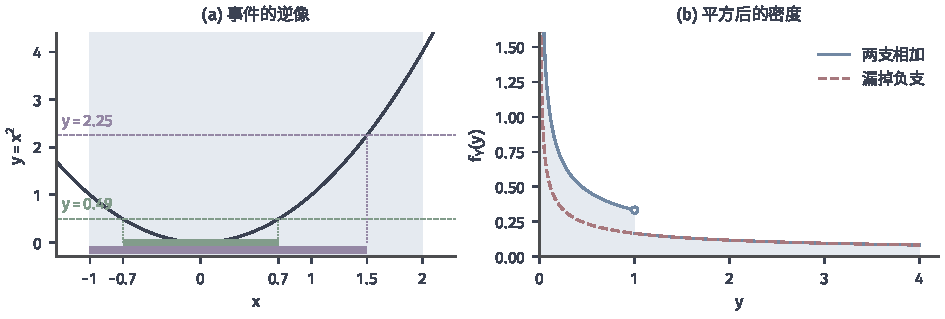
\includegraphics[width=160mm]{figures/01-basic-mathematics/05-probability-and-statistics-basics/matplotlib/prob-square-transform/figure.pdf}
  \caption{$X\sim\operatorname{U}(-1,2)$经平方$Y=X^2$的变换。(a)浅色竖带是$X$的取值范围；水平虚线是两个阈值$y$，横轴附近的粗线是事件$\{Y\leq y\}$在$X$轴上的逆像：$y=0.49$时为对称区间$[-0.7,0.7]$，$y=2.25$时左端被取值范围截断为$[-1,1.5]$。(b)$Y$的密度：在$(0,1)$上两支逆像都有贡献，密度为$1/(3\sqrt y)$；在$(1,4)$上只剩正支，密度为$1/(6\sqrt y)$，因而在$y=1$处跳降。虚线是遗漏负支时得到的错误曲线，它在$(0,1)$上少了一半，总面积只有$2/3$。}
  \label{fig:prob-square-transform}
\end{figure*}

\subsection{平移、缩放与标准化}
\label{sec:prob-standardization}

\paragraph{仿射变换的分布}
改变单位、零点或符号，都是对随机变量作仿射变换$Y=aX+b$。它是最简单的变换，也是比较不同变量、使用分布表时最常用的一步。

设$a>0$，则$aX+b\leq y$等价于$X\leq(y-b)/a$，所以$F_Y(y)=F_X\bigl((y-b)/a\bigr)$。设$a<0$，不等号方向反转，$F_Y(y)=\mathbb{P}\bigl(X\geq(y-b)/a\bigr)=1-F_X\bigl(((y-b)/a)^-\bigr)$。若$X$有密度，由定理~\ref{thm:prob-density-change}（$h(y)=(y-b)/a$，$|h'(y)|=1/|a|$）
\[
  f_Y(y)=\frac{1}{|a|}f_X\Bigl(\frac{y-b}{a}\Bigr).
\]
密度的形状不变，只是沿横轴平移、伸缩或翻转，高度同时按$1/|a|$调整以保持总面积为$1$。均值与方差按第~\ref{sec:prob-variance}节的公式变化：$\mathbb{E}[Y]=a\,\mathbb{E}[X]+b$，$\operatorname{Var}(Y)=a^2\operatorname{Var}(X)$。

例如$Z\sim\mathcal{N}(0,1)$时，$Y=\sigma Z+\mu$（$\sigma>0$）的密度是$\frac1\sigma\varphi\bigl(\frac{y-\mu}{\sigma}\bigr)$，正是$\mathcal{N}(\mu,\sigma^2)$；这验证了第~\ref{sec:prob-gaussian}节的说法。更一般地，$X\sim\mathcal{N}(\mu,\sigma^2)$且$a\neq0$时，$aX+b\sim\mathcal{N}(a\mu+b,a^2\sigma^2)$：高斯分布族在仿射变换下封闭。

$a=0$是退化情形：$Y=b$恒为常数，分布函数在$b$处从$0$跳到$1$，即使$X$有密度，$Y$也没有密度，方差为$0$。上面带$1/|a|$的密度公式在这里失效，因为所有概率都被压到了一个点上。

\paragraph{标准化}
比较不同单位、不同尺度的量时，我们常把它们换算到共同的尺度。设$X$的方差有限且$\sigma^2=\operatorname{Var}(X)>0$，均值为$\mu$。

\begin{definition}[标准化]
\label{def:prob-standardization}
称
\[
  Z=\frac{X-\mu}{\sigma}
\]
为$X$的\term{标准化}（standardization）变量。
\end{definition}

由仿射变换的公式，$\mathbb{E}[Z]=0$，$\operatorname{Var}(Z)=1$。$Z$的取值表示“偏离均值多少个标准差”，与原来的单位无关。例如两门考试的平均分与离散程度不同，一名学生在甲考试得$85$分（均值$70$、标准差$10$），在乙考试得$80$分（均值$60$、标准差$8$），标准化值分别为$1.5$与$2.5$，乙考试的相对表现更好。第~\ref{sec:prob-gaussian}节的概率计算，也正是先把高斯变量标准化，再查$\Phi$的表。

标准化只改变位置与尺度，不改变分布的形状。高斯变量标准化后是$\mathcal{N}(0,1)$，这是高斯族在仿射变换下封闭的结果；其他分布标准化后并不会变成高斯分布。$T\sim\operatorname{Exp}(1)$标准化后$Z=T-1$，取值于$[-1,\infty)$，偏度仍为$2$；$\operatorname{Bernoulli}(p)$标准化后仍只取两个值。事实上，$a>0$时偏度与峰度在仿射变换下不变，因为分子与分母中的$a$的幂次相互抵消。因此，“零均值、单位方差”与“服从标准正态分布”是两回事，使用$\Phi$的表之前必须另有理由相信变量服从或近似服从高斯分布。

\section{本章小结}
\label{sec:prob-summary}

回到章首的三个问题。掷骰子时，样本空间是$\{1,\dots,6\}$，“出现偶数点”是子集$\{2,4,6\}$，在等可能假设下其概率为$1/2$。抽检问题在“每个$10$件子集等可能”的假设下由计数求得：不放回时至少一件次品的概率约为$0.416$；若改为有放回，次品数服从二项分布，概率约为$0.401$，次品数的均值都是$0.5$。等待时间问题若采用平均$5$分钟的指数模型，等待超过$10$分钟的概率约为$0.135$，中位数约$3.5$分钟。每个答案都依赖明确的模型假设：等可能性、独立性或无记忆性，一旦假设改变，计算就要随之调整。

本章的对象之间有清楚的层次。概率给事件赋值，并由三条规则推出补事件、加法公式与连续性；条件概率与独立性描述已知信息怎样改变概率。随机变量把结果对应为数值，它的分布汇总了“取值落在哪里”的全部概率，可以统一用分布函数表示；离散变量还可以用质量函数逐点列出，有密度的变量则用密度积分计算，两者之外还有混合分布等情形。

完整分布与数值特征回答不同的问题。分布能计算任何取值范围的概率，例如等待超过$10$分钟的概率；期望、方差与分位数则把分布压缩成几个数，分别回答平均位置、波动大小与“多少比例不超过某个值”。数值特征便于报告和比较，但不能代替分布：相同的均值与方差可以对应形状截然不同的分布，均值也可能根本不存在。常见分布族由少数参数和明确的假设确定，二项与Poisson、几何与指数之间的关系说明了这些模型怎样相互联系。变换一节则说明，新变量的分布可以由原分布推前得到，计算时要先确定取值范围，并收齐所有逆像分支。

本章始终只看一个随机变量。实际问题中，我们往往同时关心几个量：抽检样本中两类缺陷各有几件、同一顾客的等待时间与服务时间、多次测量的读数。它们如何共同变化，知道一个之后另一个的分布怎样改变，它们的和与比值服从什么分布，是第~\ref{chap:random-vectors}章要回答的问题。

\chapter{随机向量与联合分布}
\label{chap:random-vectors}
\label{chap:probability-theory}

第~\ref{chap:random-variables}章每次只研究一个随机变量。实际问题却常常同时记录几个量：同一位学生考前的复习次数与考试是否通过，两台传感器对同一温度的读数，一批多分类试验中各类别出现的次数。分别写出每个量的分布，仍回答不了“两个量是否倾向于一起偏高”“知道其中一个以后，另一个的可能性怎样改变”“它们的和服从什么分布”这类问题，因为这些问题都涉及几个量在同一次试验中的共同取值。

本章研究多个随机变量的共同描述。前四节先建立联合分布、边缘分布和联合数值特征，再分别讨论独立关系与条件关系：独立表示一个变量不提供关于另一个变量的信息，条件分布则说明获得信息以后怎样重新计算概率。第五、六节方向相反：前者从已知分布出发，计算和、比值、仿射变换等组合量的分布；后者从目标分布出发，寻找能够产生它的随机输入和操作。最后一节把这些操作集中用于多元高斯分布，在一个模型里完成生成、边缘化、独立判定和条件计算。

本章沿用第~\ref{chap:random-variables}章的范围：只处理由质量函数求和或由普通密度积分计算概率的模型。多元积分、换元公式和矩阵分解分别取自第~\ref{chap:multivariate-integration}章与前面的矩阵各章。更一般的联合分布和条件分布需要测度论，可参考\BookPartRef{part:probability-spaces}{卷2《数学准备：抽象数学》的“概率空间”部分}。

\section{随机向量与联合分布}
\label{sec:rvec-joint}

研究几个量的共同取值，首先要把它们放在同一次试验里，并给“几个量同时满足某些条件”这类事件赋予概率。本节先建立这一描述，再说明怎样从中取出单个分量的分布，以及为什么反过来不行。

\subsection{随机向量与联合分布}

\paragraph{随机向量}
设$X$表示一名学生考前一周复习的次数，$Y$表示他的考试是否通过（通过记为$1$）。分别知道$X$和$Y$的分布，只能回答“复习两次的学生占多少”“通过的学生占多少”；要问“复习两次且通过的学生占多少”，就必须知道两个量在同一名学生身上怎样同时取值。

\begin{definition}[随机向量与联合分布]
设$X_1,\ldots,X_d$是定义在同一随机试验上的随机变量。把它们排成列向量
\[
 \bm X=(X_1,\ldots,X_d)^{\top},
\]
称为$d$维\term{随机向量}（random vector）。试验每进行一次，$\bm X$得到一个实现值$\bm x\in\mathbb R^d$。对$\mathbb R^d$中的集合$A$，$\{\bm X\in A\}$是一个事件；这些事件的概率$\mathbb P(\bm X\in A)$合起来称为$\bm X$的\term{联合分布}（joint distribution）。
\end{definition}

“同一随机试验”这一条件不可省略。只有当$X$和$Y$描述同一名学生、同一次测量或同一批试验时，$\{X=2,Y=1\}$才是一个有意义的事件。随机向量本身仍是随机量，实现值$\bm x$是一次观测得到的普通向量；与第~\ref{chap:random-variables}章一样，我们用大写字母表示前者，用小写字母表示后者。

\paragraph{离散情形：二维概率表}
若$X$与$Y$都只取有限个或可数个值，联合分布由
\[
 p_{X,Y}(x,y)=\mathbb P(X=x,\,Y=y)
\]
完全确定，称为\term{联合质量函数}（joint probability mass function）。它非负，对全部取值求和等于$1$；任意事件的概率等于事件所含取值对的质量之和：
\[
 \mathbb P\bigl((X,Y)\in A\bigr)=\sum_{(x,y)\in A}p_{X,Y}(x,y).
\]
两个变量各取有限个值时，联合质量函数就是一张二维概率表。

\begin{example}[复习次数与考试结果]
\label{ex:rvec-study-table}
作为教学示例，设复习次数$X\in\{0,1,2\}$与考试结果$Y\in\{0,1\}$的联合概率如图~\ref{fig:rvec-joint-table}(a)左侧的六个格子所示。复习至少一次且通过的概率是
\[
 \mathbb P(X\ge1,\,Y=1)=p_{X,Y}(1,1)+p_{X,Y}(2,1)=0.25+0.25=0.50.
\]
事件$\{X>Y\}$包含取值对$(1,0)$、$(2,0)$与$(2,1)$，故$\mathbb P(X>Y)=0.15+0.05+0.25=0.45$。计算任何联合事件，都只需在表中圈出相应格子并相加。
\end{example}

\begin{figure}[htbp]
  \centering
  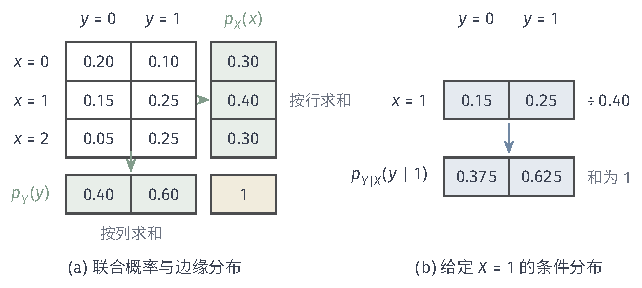
\includegraphics[width=108.8mm]{figures/01-basic-mathematics/05-probability-and-statistics-basics/tikz/rvec-joint-table/figure.pdf}
  \caption{二维概率表。(a)中白色格子是复习次数$X$与考试结果$Y$的联合概率，六个数之和为$1$；按行求和得到右侧$X$的边缘分布，按列求和得到下方$Y$的边缘分布。(b)取出$X=1$一行，除以该行之和$0.40$，得到给定$X=1$时$Y$的条件分布。}
  \label{fig:rvec-joint-table}
\end{figure}

\paragraph{连续情形：联合密度}
若$(X,Y)$的取值连续变化，单个点的概率为零，需要像一元情形那样用密度累计概率。称非负函数$f_{X,Y}$为$(X,Y)$的\term{联合密度}（joint density），如果对平面上的矩形以及第~\ref{chap:multivariate-integration}章能够积分的区域$A$，都有
\[
 \mathbb P\bigl((X,Y)\in A\bigr)=\iint_A f_{X,Y}(x,y)\,\mathrm dx\,\mathrm dy .
\]
取$A=\mathbb R^2$可知联合密度的积分为$1$。与一元情形相同，$f_{X,Y}(x,y)$本身不是概率；在$(x,y)$附近边长为$h,k$的小矩形上，概率约为$f_{X,Y}(x,y)hk$，所以联合密度表示单位面积上的概率。$d$维情形把二重积分换成$d$重积分即可。

\begin{example}[正方形上的联合密度]
\label{ex:rvec-square-density}
令$f_{X,Y}(x,y)=x+y$，$0\le x,y\le1$，其余位置为零。先检查归一化：
\[
 \int_0^1\!\!\int_0^1(x+y)\,\mathrm dy\,\mathrm dx=\int_0^1\Bigl(x+\frac12\Bigr)\mathrm dx=1 .
\]
两个分量都不超过$1/2$的概率为$\int_0^{1/2}\!\int_0^{1/2}(x+y)\,\mathrm dy\,\mathrm dx=1/8$。事件$\{X+Y\le1\}$对应三角形区域，按累次积分计算：
\[
 \mathbb P(X+Y\le1)=\int_0^1\!\!\int_0^{1-x}(x+y)\,\mathrm dy\,\mathrm dx
 =\int_0^1\frac{(1-x)(1+x)}2\,\mathrm dx=\frac13 .
\]
密度在右上角较大，所以落在左下三角形的概率小于面积比$1/2$。本章后面会多次回到这个例子。
\end{example}

\paragraph{联合分布函数}
质量函数和密度分别适用于两类模型。与一元情形一样，分布函数给出不依赖模型类型的统一描述。对$d$维随机向量定义\term{联合分布函数}（joint distribution function）
\[
 F_{\bm X}(\bm x)=\mathbb P(X_1\le x_1,\ldots,X_d\le x_d),\qquad \bm x\in\mathbb R^d .
\]
二维时，矩形概率可以由四个角上的值算出。对$a_1<b_1$、$a_2<b_2$，事件$\{X\le b_1,Y\le b_2\}$去掉$\{X\le a_1,Y\le b_2\}$和$\{X\le b_1,Y\le a_2\}$，两者的公共部分$\{X\le a_1,Y\le a_2\}$被去掉了两次，需要加回一次，于是
\[
\begin{aligned}
 &\mathbb P(a_1<X\le b_1,\,a_2<Y\le b_2)\\
 &\quad=F_{X,Y}(b_1,b_2)-F_{X,Y}(a_1,b_2)-F_{X,Y}(b_1,a_2)+F_{X,Y}(a_1,a_2).
\end{aligned}
\]
所有矩形的概率确定以后，整个联合分布也就确定了；这一结论的一般证明留到卷二。对示例~\ref{ex:rvec-square-density}，在单位正方形内
$F_{X,Y}(x,y)=\int_0^x\!\int_0^y(s+t)\,\mathrm dt\,\mathrm ds=xy(x+y)/2$，代入$x=y=1/2$又得到$1/8$。

\paragraph{多项分布}
多次类别试验的计数向量是联合质量函数的典型例子。设一次试验的结果落入$K$个类别之一，类别$k$的概率为$\pi_k$，概率向量$\bm\pi=(\pi_1,\ldots,\pi_K)^{\top}$各分量非负且和为$1$。把试验独立重复$n$次，记$N_k$为结果落入类别$k$的次数，得到计数向量$\bm N=(N_1,\ldots,N_K)^{\top}$。

给定非负整数$n_1,\ldots,n_K$且$n_1+\cdots+n_K=n$。任取一个恰有$n_k$次落入类别$k$的具体结果序列，由试验的独立性，它的概率是$\pi_1^{n_1}\cdots\pi_K^{n_K}$。这样的序列共有$n!/(n_1!\cdots n_K!)$个，即把$n$个位置分成大小为$n_1,\ldots,n_K$的$K$组的方法数（第~\ref{chap:counting}章）。各序列互斥，把概率相加就得到下面的分布。

\begin{definition}[多项分布]
称$\bm N$服从参数为$n$与$\bm\pi$的\term{多项分布}（multinomial distribution），记为$\bm N\sim\operatorname{Mult}(n,\bm\pi)$，若
\[
 \mathbb P(N_1=n_1,\ldots,N_K=n_K)=\frac{n!}{n_1!\cdots n_K!}\,\pi_1^{n_1}\cdots\pi_K^{n_K},
\]
其中$n_1,\ldots,n_K$为非负整数且$n_1+\cdots+n_K=n$；其他取值的概率为零。
\end{definition}

各分量之和恒等于$n$，这是多项分布最重要的结构：$\bm N$的取值只落在满足$\sum_kn_k=n$的整数点上。$K=2$时，$N_1$就是$n$次试验中“落入第一类”的次数，服从$\operatorname{Bin}(n,\pi_1)$，而$N_2=n-N_1$完全由$N_1$决定。

\begin{example}[三类结果的计数]
\label{ex:rvec-multinomial}
设$n=4$，$\bm\pi=(0.5,0.3,0.2)^{\top}$。恰好两次落入第一类、第二类和第三类各一次的概率为
\[
 \mathbb P\bigl(\bm N=(2,1,1)^{\top}\bigr)=\frac{4!}{2!\,1!\,1!}\,0.5^2\times0.3\times0.2=12\times0.015=0.18 .
\]
而$\mathbb P\bigl(\bm N=(2,2,1)^{\top}\bigr)=0$，因为$2+2+1\neq4$。
\end{example}

\subsection{边缘分布}

\paragraph{从联合分布求边缘分布}
有了联合分布，常常又只关心其中一部分分量，例如只问复习次数$X$本身的分布。事件$\{X=x\}$可以按$Y$的取值拆成互斥事件$\{X=x,Y=y\}$之并，由可加性，
\[
 p_X(x)=\sum_y p_{X,Y}(x,y),\qquad p_Y(y)=\sum_x p_{X,Y}(x,y).
\]
这就是二维概率表按行或按列求和。具有联合密度时，取$A=[a,b]\times\mathbb R$，并按第~\ref{chap:multivariate-integration}章的累次积分先对$y$积分（被积函数非负，无穷区间上的积分按截断取极限理解），得到
\[
 \mathbb P(a\le X\le b)=\int_a^b\Bigl(\int_{-\infty}^{\infty}f_{X,Y}(x,y)\,\mathrm dy\Bigr)\mathrm dx ,
\]
所以$f_X(x)=\int f_{X,Y}(x,y)\,\mathrm dy$是$X$的密度。这样得到的单个分量的分布称为\term{边缘分布}（marginal distribution），对其余分量求和或积分的操作称为\term{边缘化}（marginalization）。高维时同理：保留哪些分量，就对其余全部分量求和或积分。

图~\ref{fig:rvec-joint-table}(a)中，按行求和得到$p_X=(0.30,0.40,0.30)$，按列求和得到$p_Y=(0.40,0.60)$。示例~\ref{ex:rvec-square-density}中，$f_X(x)=\int_0^1(x+y)\,\mathrm dy=x+1/2$，$0\le x\le1$；由对称性，$f_Y(y)=y+1/2$。对多项分布，只看第$k$类是否出现，每次试验以概率$\pi_k$“成功”且各次独立，所以边缘分布是$N_k\sim\operatorname{Bin}(n,\pi_k)$。

\paragraph{边缘分布不能确定联合分布}
边缘化把其他分量的信息汇总掉，这一步一般不能逆转。设$X$与$Y$都等可能取$0$或$1$。第一种联合分布让四个取值对各有概率$1/4$；第二种只允许$(0,0)$与$(1,1)$，各有概率$1/2$，即$Y=X$。两张表按行、按列求和都得到$(1/2,1/2)$，边缘完全相同；但前者$\mathbb P(X=Y)=1/2$，后者$\mathbb P(X=Y)=1$。

\begin{example}[随机变号]
\label{ex:rvec-random-sign}
令$Z\sim\mathcal N(0,1)$，$S$与$Z$独立，等可能取$1$或$-1$，再令$X=Z$，$Y=SZ$。由$Z$的对称性，
\[
 \mathbb P(Y\le y)=\tfrac12\mathbb P(Z\le y)+\tfrac12\mathbb P(-Z\le y)=\Phi(y),
\]
其中$\Phi$是标准高斯分布函数，所以$Y$也服从$\mathcal N(0,1)$。图~\ref{fig:rvec-same-marginals}比较了它与两个独立标准高斯变量：上方和右侧的边缘直方图几乎一样，散点却截然不同。随机变号的散点全部落在两条对角线$|y|=|x|$上，知道$X$以后$Y$只剩两个可能值。
\end{example}

\begin{figure}[htbp]
  \centering
  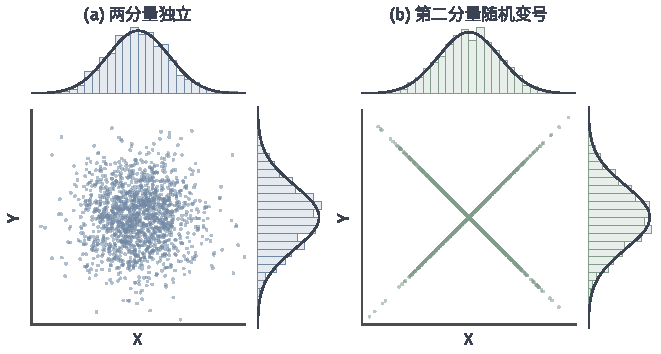
\includegraphics[width=112mm]{figures/01-basic-mathematics/05-probability-and-statistics-basics/matplotlib/rvec-same-marginals/figure.pdf}
  \caption{边缘分布相同、联合分布不同。两幅图各有$1500$个模拟点（固定随机种子）：(a)中$X,Y$是独立的标准高斯变量；(b)中$X=Z$，$Y=SZ$，$S$等可能取$\pm1$并与$Z$独立。两图上方与右侧的直方图都与标准高斯密度（黑线）吻合，但(b)的全部点落在两条对角线上。}
  \label{fig:rvec-same-marginals}
\end{figure}

因此，单独知道每个分量的分布还不足以回答涉及几个分量的问题。联合分布在边缘分布之外还记录了分量之间的联系；后面三节分别从数值特征、独立性和条件分布三个角度描述这种联系。

\section{联合分布的数值特征}
\label{sec:rvec-moments}

完整的联合分布包含很多信息，在高维时尤其难以直接列出或画出。第~\ref{chap:random-variables}章用期望和方差概括单个分布的位置与波动；对随机向量，我们还需要一个量来概括分量之间怎样一起变化。

\subsection{均值向量}

\paragraph{定义与线性性}
随机向量的中心位置可以逐个分量描述。设每个分量都有有限期望，即$\mathbb E|X_i|<\infty$，定义\term{均值向量}（mean vector）
\[
 \bm\mu=\mathbb E\bm X=(\mathbb EX_1,\ldots,\mathbb EX_d)^{\top}.
\]
每个$\mathbb EX_i$只依赖$X_i$的边缘分布，也可以直接对联合分布计算：与一元情形相同，函数$g(\bm X)$的期望按
\[
 \mathbb E\,g(\bm X)=\sum_{\bm x}g(\bm x)p_{\bm X}(\bm x)
 \quad\text{或}\quad
 \mathbb E\,g(\bm X)=\int_{\mathbb R^d}g(\bm x)f_{\bm X}(\bm x)\,\mathrm d\bm x
\]
计算，只要求和或积分绝对收敛，无须先求出$g(\bm X)$的分布。取$g(x,y)=x+y$，把求和拆成两项，
\[
 \mathbb E(X+Y)=\sum_{x,y}x\,p_{X,Y}(x,y)+\sum_{x,y}y\,p_{X,Y}(x,y)=\mathbb EX+\mathbb EY .
\]
积分情形相同。由此，对常向量$\bm a$、常数$b$以及$m\times d$常矩阵$\bm A$、常向量$\bm b$，
\[
 \mathbb E(\bm a^{\top}\bm X+b)=\bm a^{\top}\bm\mu+b,\qquad
 \mathbb E(\bm A\bm X+\bm b)=\bm A\bm\mu+\bm b .
\]
第二式逐行使用第一式即得。这些等式不需要分量之间有任何独立性。

\paragraph{均值只描述中心}
示例~\ref{ex:rvec-study-table}中$\mathbb EX=0\times0.3+1\times0.4+2\times0.3=1$，$\mathbb EY=0.6$，故$\bm\mu=(1,0.6)^{\top}$；示例~\ref{ex:rvec-square-density}中$\mathbb EX=\int_0^1x(x+1/2)\,\mathrm dx=7/12$，由对称性$\bm\mu=(7/12,7/12)^{\top}$。

均值向量给出共同的中心位置，却没有说明分量怎样一起变化。回到上一小节两个边缘相同的二元例子：两种联合分布的均值向量都是$(1/2,1/2)^{\top}$。但在独立的那张表中，$X+Y$以概率$1/4,1/2,1/4$取$0,1,2$，方差为$1/2$；在$Y=X$的那张表中，$X+Y$等可能取$0$或$2$，方差为$1$。两个读数同时偏高或同时偏低时，和的波动更大，这需要一个新的数值特征来描述。

\subsection{协方差与相关系数}

\paragraph{协方差}
把和的方差展开，就能看出缺少的是哪一项。记$\mu_X=\mathbb EX$，$\mu_Y=\mathbb EY$，则
\[
\begin{aligned}
 \operatorname{Var}(X+Y)&=\mathbb E\bigl[(X-\mu_X)+(Y-\mu_Y)\bigr]^2\\
 &=\operatorname{Var}(X)+\operatorname{Var}(Y)+2\,\mathbb E\bigl[(X-\mu_X)(Y-\mu_Y)\bigr].
\end{aligned}
\]
前两项只依赖边缘分布，最后一项则依赖联合分布。

\begin{definition}[协方差]
设$\mathbb EX^2<\infty$，$\mathbb EY^2<\infty$。称
\[
 \operatorname{Cov}(X,Y)=\mathbb E\bigl[(X-\mu_X)(Y-\mu_Y)\bigr]
\]
为$X$与$Y$的\term{协方差}（covariance）。
\end{definition}

有限二阶矩保证这个期望有限：由$|uv|\le(u^2+v^2)/2$，中心化乘积的绝对值被两个平方项控制。展开乘积并用期望的线性性，得到常用的计算公式
\[
 \operatorname{Cov}(X,Y)=\mathbb E[XY]-\mu_X\mu_Y .
\]
中心化乘积$(X-\mu_X)(Y-\mu_Y)$在两个变量同时高于或同时低于各自均值时为正，一高一低时为负。协方差为正，表示“同向偏离”在概率加权下占优势；为负则表示“反向偏离”占优势。

协方差对每个变量都是线性的，并且不受平移影响：$\operatorname{Cov}(aX+b,cY+e)=ac\operatorname{Cov}(X,Y)$，$\operatorname{Cov}(X_1+X_2,Y)=\operatorname{Cov}(X_1,Y)+\operatorname{Cov}(X_2,Y)$；还有$\operatorname{Cov}(X,X)=\operatorname{Var}(X)$。于是开头的展开式推广为
\begin{equation}
 \operatorname{Var}(aX+bY)=a^2\operatorname{Var}(X)+b^2\operatorname{Var}(Y)+2ab\operatorname{Cov}(X,Y).
 \label{eq:rvec-variance-of-combination}
\end{equation}

\begin{example}[概率表中的协方差]
\label{ex:rvec-table-covariance}
对示例~\ref{ex:rvec-study-table}，$XY$只在$(1,1)$与$(2,1)$处非零，
\[
 \mathbb E[XY]=1\times0.25+2\times0.25=0.75,\qquad
 \operatorname{Cov}(X,Y)=0.75-0.6=0.15,
\]
复习次数多与考试通过倾向于同时出现。对上一小节$Y=X$的二元例子，$\operatorname{Cov}(X,Y)=\operatorname{Var}(X)=1/4$，代入式~\eqref{eq:rvec-variance-of-combination}得$\operatorname{Var}(X+Y)=1/4+1/4+2\times1/4=1$，与直接计算一致。
\end{example}

\paragraph{相关系数}
协方差的数值依赖单位：把$X$由米改成厘米，协方差扩大$100$倍，而两个量的联系并没有改变。用两个标准差$\sigma_X,\sigma_Y$去除，就得到与单位无关的量。

\begin{definition}[相关系数]
设$0<\operatorname{Var}(X)<\infty$，$0<\operatorname{Var}(Y)<\infty$。称
\[
 \operatorname{Corr}(X,Y)=\frac{\operatorname{Cov}(X,Y)}{\sigma_X\sigma_Y}
\]
为$X$与$Y$的\term{相关系数}（correlation coefficient），常记为$\rho_{X,Y}$或$\rho$。
\end{definition}

\begin{theorem}[相关系数的范围]
\label{thm:rvec-correlation-bound}
在上述条件下，$-1\le\rho_{X,Y}\le1$。并且$|\rho_{X,Y}|=1$当且仅当存在常数$a$与$b\neq0$，使$Y=a+bX$以概率$1$成立，此时$b$与$\rho_{X,Y}$同号。
\end{theorem}

\begin{proof}
令$U=(X-\mu_X)/\sigma_X$，$V=(Y-\mu_Y)/\sigma_Y$为两个标准化变量，则$\mathbb EU^2=\mathbb EV^2=1$，$\mathbb E[UV]=\rho$。对平方的期望展开，
\[
 0\le\mathbb E(V-\rho U)^2=\mathbb EV^2-2\rho\,\mathbb E[UV]+\rho^2\mathbb EU^2=1-\rho^2 ,
\]
故$\rho^2\le1$。若$\rho^2=1$，非负随机变量$(V-\rho U)^2$的期望为零。一个非负随机变量若以正概率不小于某个$\varepsilon>0$，它的期望至少是$\varepsilon$乘以这个概率，必然为正；所以$(V-\rho U)^2$以概率$1$为零，即$V=\rho U$。代回$U,V$的定义，$Y=\mu_Y+\rho\frac{\sigma_Y}{\sigma_X}(X-\mu_X)$，斜率与$\rho$同号。反过来，若$Y=a+bX$且$b\neq0$，则$\operatorname{Cov}(X,Y)=b\sigma_X^2$，$\sigma_Y=|b|\sigma_X$，于是$\rho=b/|b|=\pm1$。
\end{proof}

这个证明与第~\ref{chap:normed-inner-product-spaces}章的Cauchy--Schwarz不等式（定理~\ref{thm:linear-algebra-cauchy-schwarz}）是同一个论证：把$\mathbb E[UV]$看作内积，相关系数就是两个中心化变量夹角的余弦。若某个变量方差为零，它以概率$1$等于常数，与任何变量的协方差都是零，相关系数的分母为零而没有定义；这时谈论“共同变化”本来就没有意义。

相关系数刻画的是散点向一条直线集中的程度，而不是直线的斜率。图~\ref{fig:rvec-correlation}前三幅中，$\rho=0.9$的点紧贴一条上升直线，$\rho=-0.6$的点较松散地沿下降方向分布，$\rho=0$的点看不出线性趋势。第四幅中$Y$几乎由$X$决定，相关系数却接近零，因为抛物线的左右两支对“同向”和“反向”的贡献互相抵消。相关系数主要描述线性关联，第~\ref{sec:rvec-independence}节还会回到这个例子。

\begin{figure}[htbp]
  \centering
  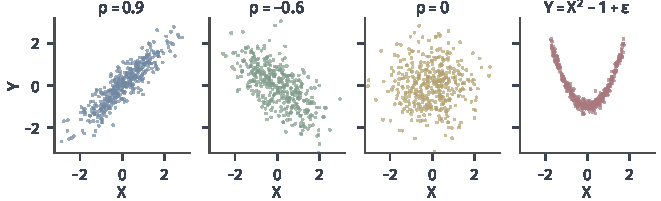
\includegraphics[width=112mm]{figures/01-basic-mathematics/05-probability-and-statistics-basics/matplotlib/rvec-correlation/figure.pdf}
  \caption{不同相关系数下的散点，每幅$400$个模拟点（固定随机种子）。前三幅中$X$与$Y$都是标准高斯变量，相关系数分别为$0.9$、$-0.6$和$0$。第四幅中$X$在$[-\sqrt3,\sqrt3]$上均匀分布，$Y=X^2-1$再加小噪声，相关系数为零，但$Y$几乎由$X$决定。}
  \label{fig:rvec-correlation}
\end{figure}

\begin{example}[两个例子的相关系数]
\label{ex:rvec-correlation-values}
示例~\ref{ex:rvec-study-table}中$\operatorname{Var}(X)=\mathbb EX^2-1=(0.4+4\times0.3)-1=0.6$，$\operatorname{Var}(Y)=0.6\times0.4=0.24$，故
$\rho=0.15/\sqrt{0.6\times0.24}\approx0.40$。

示例~\ref{ex:rvec-square-density}中，$\mathbb E[XY]=\int_0^1\!\int_0^1xy(x+y)\,\mathrm dy\,\mathrm dx=1/3$，$\mathbb EX^2=\int_0^1x^2(x+1/2)\,\mathrm dx=5/12$。于是
\[
 \operatorname{Cov}(X,Y)=\frac13-\Bigl(\frac7{12}\Bigr)^2=-\frac1{144},\qquad
 \operatorname{Var}(X)=\frac5{12}-\frac{49}{144}=\frac{11}{144},
\]
相关系数为$-1/11\approx-0.09$。密度$x+y$在两个分量都大时较大，看起来像“同向”，但在这个密度下，一个分量偏大时，另一个分量的条件分布会向下移动（第~\ref{sec:rvec-conditioning}节会算出这一点），总体上呈现微弱的负相关。直观印象需要通过计算核对。
\end{example}

\subsection{协方差矩阵}
\label{sec:rvec-covariance-matrix}

\paragraph{定义与半正定性}
$d$个分量两两之间都有协方差，把它们排成矩阵便于统一计算。设各分量二阶矩有限，定义\term{协方差矩阵}（covariance matrix）
\[
 \bm\Sigma=\operatorname{Cov}(\bm X)=\mathbb E\bigl[(\bm X-\bm\mu)(\bm X-\bm\mu)^{\top}\bigr],
 \qquad \bm\Sigma_{i,j}=\operatorname{Cov}(X_i,X_j),
\]
其中矩阵的期望逐元素计算。对角元是各分量的方差，非对角元是协方差。

\begin{theorem}[协方差矩阵的性质]
\label{thm:rvec-covariance-psd}
协方差矩阵对称半正定。对任意常向量$\bm a,\bm b\in\mathbb R^d$，
\[
 \operatorname{Var}(\bm a^{\top}\bm X)=\bm a^{\top}\bm\Sigma\bm a\ge0,\qquad
 \operatorname{Cov}(\bm a^{\top}\bm X,\bm b^{\top}\bm X)=\bm a^{\top}\bm\Sigma\bm b .
\]
\end{theorem}

\begin{proof}
对称性来自$\operatorname{Cov}(X_i,X_j)=\operatorname{Cov}(X_j,X_i)$。由均值向量的线性性，$\bm a^{\top}\bm X-\mathbb E(\bm a^{\top}\bm X)=\bm a^{\top}(\bm X-\bm\mu)$，同理处理$\bm b$。两个标量相乘可写成
\[
 \bm a^{\top}(\bm X-\bm\mu)\,(\bm X-\bm\mu)^{\top}\bm b ,
\]
它是矩阵$(\bm X-\bm\mu)(\bm X-\bm\mu)^{\top}$各元素的线性组合，取期望后得到$\bm a^{\top}\bm\Sigma\bm b$。取$\bm b=\bm a$得方差公式；方差非负，所以$\bm\Sigma$半正定。
\end{proof}

这个定理把任意线性组合的方差交给一个矩阵计算，式~\eqref{eq:rvec-variance-of-combination}是$d=2$的特例。示例~\ref{ex:rvec-study-table}中
\[
 \bm\Sigma=\begin{bmatrix}0.6&0.15\\0.15&0.24\end{bmatrix}.
\]
例如取$\bm a=(1,-2)^{\top}$，得$\operatorname{Var}(X-2Y)=\bm a^{\top}\bm\Sigma\bm a=0.6-4\times0.15+4\times0.24=0.96$。

\paragraph{多项计数的负协方差}
多项分布的计数之和固定，这个约束会体现在协方差上。由边缘分布$N_k\sim\operatorname{Bin}(n,\pi_k)$，$\operatorname{Var}(N_k)=n\pi_k(1-\pi_k)$。对$j\neq k$，把类别$j$与$k$合并成一类，$N_j+N_k$就是$n$次试验中落入合并类别的次数，服从$\operatorname{Bin}(n,\pi_j+\pi_k)$。由式~\eqref{eq:rvec-variance-of-combination}，
\[
 n(\pi_j+\pi_k)(1-\pi_j-\pi_k)=n\pi_j(1-\pi_j)+n\pi_k(1-\pi_k)+2\operatorname{Cov}(N_j,N_k).
\]
展开左边并消去相同项，得到
\[
 \operatorname{Cov}(N_j,N_k)=-n\pi_j\pi_k ,\qquad
 \bm\Sigma=n\bigl(\operatorname{diag}(\bm\pi)-\bm\pi\bm\pi^{\top}\bigr).
\]
协方差为负的原因很直接：总次数固定，某一类多出现一次，其余类别可分配的次数就少一次。示例~\ref{ex:rvec-multinomial}的参数给出
\[
 \bm\Sigma=\begin{bmatrix}1&-0.6&-0.4\\-0.6&0.84&-0.24\\-0.4&-0.24&0.64\end{bmatrix},
\]
每行之和都是零。

\paragraph{退化与线性关系}
行和为零说明$\bm\Sigma\bm 1=\bm0$，其中$\bm1$是全一向量。按定理~\ref{thm:rvec-covariance-psd}，$\operatorname{Var}(\bm1^{\top}\bm N)=\bm1^{\top}\bm\Sigma\bm1=0$，这正是$N_1+\cdots+N_K=n$恒成立。一般地，若$\bm a\neq\bm0$使$\bm a^{\top}\bm\Sigma\bm a=0$，则$\bm a^{\top}\bm X$方差为零，由定理~\ref{thm:rvec-correlation-bound}证明中的论证，它以概率$1$等于常数$\bm a^{\top}\bm\mu$。因此，协方差矩阵奇异，恰好对应分量之间以概率$1$成立的线性关系；这时$\bm X$的取值集中在一个超平面上。超平面在$\mathbb R^d$中的体积为零，任何联合密度在其上的积分都为零，所以这样的$\bm X$不可能有$d$维联合密度。

\section{随机变量的独立性}
\label{sec:rvec-independence}

联合分布中最简单的一种结构，是知道一个变量的取值完全不改变另一个变量的概率。第~\ref{sec:prob-event-independence}节已经对事件定义了独立性；本节把它推广到随机变量，并比较它与不相关的区别。

\subsection{独立性的定义与判定}

\paragraph{定义}
随机变量的独立应当意味着：关于$X$的任何事件与关于$Y$的任何事件都相互独立。

\begin{definition}[随机变量的独立性]
称随机变量$X$与$Y$\term{独立}（independent），记为$X\perp Y$，如果对所有能够计算概率的实数集合$A,B$（例如区间及其有限并），
\[
 \mathbb P(X\in A,\,Y\in B)=\mathbb P(X\in A)\,\mathbb P(Y\in B).
\]
\end{definition}

把$X,Y$换成随机向量、$A,B$换成相应维数空间中的集合，就得到两个随机向量独立的定义，下面的判定也照样成立。当$\mathbb P(X\in A)>0$时，等式等价于$\mathbb P(Y\in B\mid X\in A)=\mathbb P(Y\in B)$：无论得知$X$落在哪个范围，$Y$的概率都不变。这个定义对每一对集合都要检查，实际判定时通常改用质量函数或密度。

\begin{theorem}[独立性的判定]
\label{thm:rvec-independence-criteria}
\begin{enumerate}
 \item 若$X,Y$是离散随机变量，则$X\perp Y$当且仅当对所有$x,y$，$p_{X,Y}(x,y)=p_X(x)p_Y(y)$。
 \item 若$(X,Y)$具有联合密度，则$X\perp Y$当且仅当$f_X(x)f_Y(y)$也是$(X,Y)$的联合密度，即可以取$f_{X,Y}(x,y)=f_X(x)f_Y(y)$。
\end{enumerate}
\end{theorem}

\begin{proof}
离散情形。必要性取$A=\{x\}$，$B=\{y\}$即可。充分性：
\[
 \mathbb P(X\in A,Y\in B)=\sum_{x\in A}\sum_{y\in B}p_X(x)p_Y(y)
 =\Bigl(\sum_{x\in A}p_X(x)\Bigr)\Bigl(\sum_{y\in B}p_Y(y)\Bigr).
\]
密度情形。若$f_{X,Y}=f_Xf_Y$，对区间$A,B$按累次积分，
\[
 \iint_{A\times B}f_X(x)f_Y(y)\,\mathrm dx\,\mathrm dy=\int_Af_X(x)\,\mathrm dx\int_Bf_Y(y)\,\mathrm dy ,
\]
这正是独立性的等式；有限并的情形逐块相加。反过来，若$X\perp Y$，则对任意矩形，
\[
 \mathbb P(a_1<X\le b_1,\,a_2<Y\le b_2)=\int_{a_1}^{b_1}f_X(x)\,\mathrm dx\int_{a_2}^{b_2}f_Y(y)\,\mathrm dy ,
\]
即函数$f_Xf_Y$给出与$(X,Y)$相同的矩形概率，因而可以作为联合密度。
\end{proof}

密度只在不影响任何积分的个别点或曲线上可以任意改动，所以第二条说的是“可以取成乘积”，而不是要求在每一点都相等。

\paragraph{按乘积形式判别}
实际判别时，常检查联合密度能否在整个平面上写成两个非负函数之积$g(x)h(y)$。若能，那么分别对$y$和$x$积分可知$f_X$与$g$、$f_Y$与$h$只差常数因子，两个常数之积为$1$，因而$X\perp Y$。例如在$x,y>0$上$f_{X,Y}(x,y)=6e^{-2x-3y}$，它可写成$2e^{-2x}$与$3e^{-3y}$之积，所以$X\sim\operatorname{Exp}(2)$与$Y\sim\operatorname{Exp}(3)$独立。

乘积分解必须连同取值范围一起检查。设$(X,Y)$在三角形$\{0<y<x<1\}$上均匀分布，密度在三角形内恒为$2$，看起来不含$x$与$y$的交叉项。但边缘密度为$f_X(x)=2x$，$f_Y(y)=2(1-y)$；在点$(1/4,3/4)$处联合密度为零，乘积却是$1/2\times1/2=1/4$。整块取值范围不是乘积形状时，指示函数$\mathbb{I}\{y<x\}$本身就是不能分开的交叉项。离散情形同理：图~\ref{fig:rvec-joint-table}中$p_{X,Y}(0,0)=0.20$，而$p_X(0)p_Y(0)=0.3\times0.4=0.12$，所以复习次数与考试结果不独立。

\paragraph{函数变换与乘积的期望}
独立性经过各自的函数变换后仍然保持。设$X\perp Y$，$g,h$为实函数。记$g^{-1}(A)=\{x:g(x)\in A\}$，则
\[
\begin{aligned}
 \mathbb P\bigl(g(X)\in A,\,h(Y)\in B\bigr)&=\mathbb P\bigl(X\in g^{-1}(A),\,Y\in h^{-1}(B)\bigr)\\
 &=\mathbb P\bigl(g(X)\in A\bigr)\,\mathbb P\bigl(h(Y)\in B\bigr),
\end{aligned}
\]
只要这些原像集合仍在我们能计算概率的范围内。例如$X^2$与$e^{Y}$独立。

\begin{theorem}[独立变量乘积的期望]
\label{thm:rvec-product-expectation}
设$X\perp Y$，$\mathbb E|g(X)|<\infty$，$\mathbb E|h(Y)|<\infty$。则$g(X)h(Y)$的期望有限，且
\[
 \mathbb E\bigl[g(X)h(Y)\bigr]=\mathbb E\,g(X)\;\mathbb E\,h(Y).
\]
\end{theorem}

\begin{proof}
离散情形，由独立性的判定，
\[
\begin{aligned}
 \mathbb E\bigl[g(X)h(Y)\bigr]&=\sum_x\sum_yg(x)h(y)p_X(x)p_Y(y)\\
 &=\Bigl(\sum_xg(x)p_X(x)\Bigr)\Bigl(\sum_yh(y)p_Y(y)\Bigr).
\end{aligned}
\]
先对绝对值做同样的计算，得到$\mathbb E|g(X)h(Y)|=\mathbb E|g(X)|\,\mathbb E|h(Y)|<\infty$；二重级数绝对收敛，才允许上面重新排列求和次序。密度情形把求和换成累次积分，论证相同。
\end{proof}

只知道乘积$g(X)h(Y)$的期望有限是不够的：若$g\equiv0$，乘积期望为零，而$\mathbb E\,h(Y)$可能根本不存在，右边就没有意义。对上面的指数例子，$\mathbb E[XY^2]=\mathbb EX\cdot\mathbb EY^2=\frac12\times\frac2{9}=\frac19$，其中用到$Y\sim\operatorname{Exp}(3)$时$\mathbb EY^2=2/3^2$。

\subsection{两两独立与相互独立}

\paragraph{多个变量的独立}
多个变量时，有两种自然但强弱不同的要求。

\begin{definition}[相互独立与两两独立]
称随机变量$X_1,\ldots,X_n$\term{相互独立}（mutually independent），如果对所有能够计算概率的实数集合$A_1,\ldots,A_n$，
\[
 \mathbb P(X_1\in A_1,\ldots,X_n\in A_n)=\prod_{i=1}^n\mathbb P(X_i\in A_i).
\]
若只要求其中每一对变量独立，称它们\term{两两独立}（pairwise independent）。
\end{definition}

在相互独立的等式中取部分$A_i=\mathbb R$，相应因子变成$1$，就得到任意一部分变量的乘积关系。这与第~\ref{sec:prob-event-independence}节对事件“所有子组都满足乘法关系”的要求一致，所以相互独立蕴含两两独立。离散或密度模型中，相互独立等价于联合质量函数或联合密度可以取成$n$个边缘的乘积，证明与定理~\ref{thm:rvec-independence-criteria}相同。今后说“独立同分布”的变量，指的总是相互独立。

相互独立还有一个常用推论：把变量分成互不相交的几组，各组的函数仍相互独立。以离散情形为例，若$X_1,X_2,X_3$相互独立，则
\[
\begin{aligned}
 \mathbb P\bigl(X_1+X_2=s,\,X_3=v\bigr)&=\sum_{x_1+x_2=s}p_{X_1}(x_1)p_{X_2}(x_2)p_{X_3}(v)\\
 &=\mathbb P(X_1+X_2=s)\,\mathbb P(X_3=v),
\end{aligned}
\]
所以$X_1+X_2\perp X_3$。第~\ref{sec:rvec-transforms}节按这种方式逐个累加独立变量。

\paragraph{异或反例}
两两独立却不能保证相互独立。令$X,Y$独立，都等可能取$0$或$1$，再令$Z=X\oplus Y$为两者的\term{异或}（exclusive OR）：$X,Y$相同时$Z=0$，不同时$Z=1$。四种等可能结果列在表~\ref{tab:rvec-xor}中。

\begin{table}[htbp]
  \centering
  \caption{异或构造的四种等可能结果。任意两列取遍四种组合各一次，第三列却由前两列唯一确定。}
  \label{tab:rvec-xor}
  \begin{tabular}{cccc}
    \toprule
    $X$ & $Y$ & $Z=X\oplus Y$ & 概率\\
    \midrule
    $0$ & $0$ & $0$ & $1/4$\\
    $0$ & $1$ & $1$ & $1/4$\\
    $1$ & $0$ & $1$ & $1/4$\\
    $1$ & $1$ & $0$ & $1/4$\\
    \bottomrule
  \end{tabular}
\end{table}

逐对检查。$Z$取$0$与$1$各有两行，故$\mathbb P(Z=1)=1/2$。$(X,Y)$独立是假设。对$(X,Z)$，表中$(X,Z)$的四种组合$(0,0),(0,1),(1,1),(1,0)$各出现一次，所以$\mathbb P(X=x,Z=z)=1/4=\mathbb P(X=x)\mathbb P(Z=z)$；$(Y,Z)$同理。三个变量因此两两独立。但
\[
 \mathbb P(X=1,Y=1,Z=1)=0\neq\frac18=\mathbb P(X=1)\mathbb P(Y=1)\mathbb P(Z=1),
\]
三者不相互独立。单看$X$或单看$Y$，都得不到关于$Z$的任何信息；两者合在一起却完全决定$Z$。分类问题中，两个特征各自与类别无关、合起来却决定类别，正是这种结构。

\subsection{独立与不相关}

\paragraph{独立推出不相关}
协方差为零的两个变量称为\term{不相关}（uncorrelated）。独立性比它强。

\begin{theorem}[独立变量不相关]
\label{thm:rvec-independent-uncorrelated}
若$X\perp Y$且二者二阶矩有限，则$\operatorname{Cov}(X,Y)=0$。
\end{theorem}

\begin{proof}
二阶矩有限蕴含$\mathbb E|X-\mu_X|<\infty$与$\mathbb E|Y-\mu_Y|<\infty$。对$g(x)=x-\mu_X$、$h(y)=y-\mu_Y$用定理~\ref{thm:rvec-product-expectation}，
$\operatorname{Cov}(X,Y)=\mathbb E[X-\mu_X]\,\mathbb E[Y-\mu_Y]=0\cdot0=0$。
\end{proof}

在定理~\ref{thm:rvec-covariance-psd}中取$\bm a$为全一向量，$\operatorname{Var}(X_1+\cdots+X_n)$等于全部方差与全部协方差之和；因此两两不相关的变量满足$\operatorname{Var}(X_1+\cdots+X_n)=\operatorname{Var}(X_1)+\cdots+\operatorname{Var}(X_n)$。这里只需要每一对协方差为零，两两独立已经足够。例如$n$个独立$\operatorname{Bernoulli}(p)$变量之和的方差为$np(1-p)$，与第~\ref{sec:prob-discrete-models}节二项分布的方差一致。

\paragraph{不相关不推出独立}
反方向一般不成立。令$X$在$\{-1,0,1\}$上等可能取值，$Y=X^2$。由对称性$\mathbb EX=\mathbb EX^3=0$，所以
\[
 \operatorname{Cov}(X,Y)=\mathbb E[X^3]-\mathbb EX\,\mathbb EX^2=0 .
\]
但$\mathbb P(X=0,Y=0)=1/3$，而$\mathbb P(X=0)\mathbb P(Y=0)=1/3\times1/3=1/9$，二者不独立；实际上$Y$由$X$完全决定。同样的论证适用于任何关于零对称、三阶矩有限的$X$。图~\ref{fig:rvec-correlation}第四幅就是连续版本：抽到的$X$越远离零，$Y$越大，这种依赖对正负两侧是对称的，没有“$X$增大时$Y$随之增大或减小”的线性趋势，协方差把它完全漏掉了。

因此，协方差为零只排除了线性关联。只有在额外的模型假设下，例如第~\ref{sec:rvec-gaussian}节的联合高斯条件，不相关才能推出独立。

\section{条件概率与条件分布}
\label{sec:rvec-conditioning}
\label{sec:rv-conditional-distribution}

独立表示一个变量不提供关于另一个变量的信息。多数情况下并非如此：得知学生复习了两次，他通过考试的概率就应当提高。本节先在事件层面建立汇总与反推的两个公式，再把条件概率推广为条件分布，并研究条件分布的均值、方差以及条件独立。

\subsection{全概率公式与Bayes公式}
\label{sec:rvec-bayes-formula}

\paragraph{全概率公式}
回顾第~\ref{sec:prob-conditional-probability}节：$\mathbb P(B)>0$时，$\mathbb P(A\mid B)=\mathbb P(A\cap B)/\mathbb P(B)$，由此得到乘法公式$\mathbb P(A\cap B)=\mathbb P(A\mid B)\mathbb P(B)$。设某工厂的产品来自三条产线，各产线的产量占比和次品率都已知，我们想知道任取一件产品是次品的概率。这类问题的共同结构是：总体被分成若干互斥的情形，每种情形下的条件概率已知，需要把它们汇总起来。

\begin{theorem}[全概率公式]
\label{thm:rvec-total-probability}
设事件$B_1,\ldots,B_m$两两互斥，并集为整个样本空间，且每个$\mathbb P(B_i)>0$。则对任意事件$A$，
\[
 \mathbb P(A)=\sum_{i=1}^m\mathbb P(A\mid B_i)\,\mathbb P(B_i).
\]
\end{theorem}

\begin{proof}
$B_1,\ldots,B_m$覆盖全部结果且互不相交，所以$A=\bigcup_i(A\cap B_i)$，各部分互斥。由可加性$\mathbb P(A)=\sum_i\mathbb P(A\cap B_i)$，再对每一项用乘法公式即得。
\end{proof}

这个公式称为\term{全概率公式}（law of total probability）。可数多个情形时，可数可加性给出同样的结论。它把一个不易直接计算的概率，拆成“先确定处于哪种情形，再在该情形下计算”的加权平均。

\begin{example}[三条产线的次品率]
\label{ex:rvec-production-lines}
设产品来自三条产线，记事件$B_k$为“产品来自第$k$条产线”，$D$为“产品是次品”。产量占比为$\mathbb P(B_1)=0.5$、$\mathbb P(B_2)=0.3$、$\mathbb P(B_3)=0.2$，次品率为$\mathbb P(D\mid B_1)=0.01$、$\mathbb P(D\mid B_2)=0.02$、$\mathbb P(D\mid B_3)=0.04$（教学数据）。由全概率公式，
\[
 \mathbb P(D)=0.5\times0.01+0.3\times0.02+0.2\times0.04=0.005+0.006+0.008=0.019 .
\]
图~\ref{fig:rvec-bayes-tree}把这个计算画成树：每条路径上的概率相乘，得到“来自某产线且是次品”的概率，再把三条次品路径相加。
\end{example}

\begin{figure*}[htbp]
  \centering
  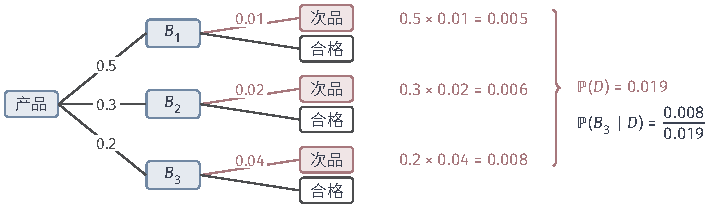
\includegraphics[width=121.6mm]{figures/01-basic-mathematics/05-probability-and-statistics-basics/tikz/rvec-bayes-tree/figure.pdf}
  \caption{全概率公式与Bayes公式的树状图。第一层分支是产品来自三条产线的概率，第二层是各产线的次品率。沿路径相乘得到三个联合概率$\mathbb P(B_k\cap D)$，相加得到$\mathbb P(D)=0.019$；其中第三条路径所占的比例就是$\mathbb P(B_3\mid D)$。}
  \label{fig:rvec-bayes-tree}
\end{figure*}

\paragraph{Bayes公式}
全概率公式由原因推出结果。实际中常常需要反过来问：已经发现一件次品，它来自第三条产线的概率是多少？已知的是$\mathbb P(D\mid B_k)$，要求的是方向相反的$\mathbb P(B_k\mid D)$。

\begin{theorem}[Bayes公式]
\label{thm:rvec-bayes}
在定理~\ref{thm:rvec-total-probability}的条件下，若$\mathbb P(A)>0$，则对每个$j$，
\[
 \mathbb P(B_j\mid A)=\frac{\mathbb P(A\mid B_j)\,\mathbb P(B_j)}{\sum_{i=1}^m\mathbb P(A\mid B_i)\,\mathbb P(B_i)} .
\]
\end{theorem}

\begin{proof}
由条件概率的定义与乘法公式，
\[
 \mathbb P(B_j\mid A)=\frac{\mathbb P(A\cap B_j)}{\mathbb P(A)}=\frac{\mathbb P(A\mid B_j)\,\mathbb P(B_j)}{\mathbb P(A)} ,
\]
再用全概率公式展开分母。
\end{proof}

这个公式称为\term{Bayes公式}（Bayes' formula）。$\mathbb P(B_j)$是观测之前对各情形的概率，称为\term{先验概率}（prior probability）；$\mathbb P(B_j\mid A)$是得知$A$发生后重新计算的概率，称为\term{后验概率}（posterior probability）。公式说明：后验概率正比于“先验概率乘以该情形下观测到$A$的概率”，分母只负责归一化，使全部后验概率之和为$1$。

\begin{example}[次品来自哪条产线]
\label{ex:rvec-production-bayes}
续示例~\ref{ex:rvec-production-lines}。三条次品路径的概率是$0.005$、$0.006$、$0.008$，除以总和$0.019$，
\[
 \mathbb P(B_1\mid D)\approx0.263,\qquad \mathbb P(B_2\mid D)\approx0.316,\qquad \mathbb P(B_3\mid D)\approx0.421 .
\]
第三条产线只生产两成产品，却贡献了四成以上的次品，因为它的次品率最高。分母必须汇总全部情形：若计算时漏掉第二条产线，会误得$\mathbb P(B_3\mid D)=0.008/0.013\approx0.615$。被漏掉的情形同样可能产生次品，它的贡献不计入分母，其余情形的后验概率就被系统地高估。
\end{example}

先验概率的影响有时与直觉相差很大。设某种疾病的患病率为$1\%$，检测对患者呈阳性的概率为$0.9$，对未患病者误报阳性的概率为$0.05$。阳性的概率为$0.01\times0.9+0.99\times0.05=0.0585$，于是阳性者确实患病的概率只有$0.009/0.0585\approx0.154$。检测本身相当灵敏，但未患病的人数是患者的$99$倍，他们中少量的误报在阳性结果里仍占多数。

\subsection{条件分布}

\paragraph{离散情形：按行归一化}
把条件概率用于随机变量的取值事件，就得到条件分布。对离散变量，只要$p_X(x)>0$，事件$\{X=x\}$有正概率，可以直接定义
\[
 p_{Y\mid X}(y\mid x)=\mathbb P(Y=y\mid X=x)=\frac{p_{X,Y}(x,y)}{p_X(x)} .
\]
固定$x$，它对$y$非负且和为$1$，是一个质量函数，称为给定$X=x$时$Y$的\term{条件分布}（conditional distribution），$p_{Y\mid X}$称为\term{条件质量函数}（conditional probability mass function）。在二维概率表中，这就是取出$X=x$那一行，再除以该行之和，如图~\ref{fig:rvec-joint-table}(b)所示。

对示例~\ref{ex:rvec-study-table}，三行归一化后，给定$X=0,1,2$时$Y=1$的条件概率依次为
\[
 \frac{0.10}{0.30}=\frac13,\qquad \frac{0.25}{0.40}=0.625,\qquad \frac{0.25}{0.30}=\frac56 .
\]
无条件时$\mathbb P(Y=1)=0.6$；得知复习次数以后，这个概率在$1/3$到$5/6$之间变化。这正是$X$与$Y$不独立的表现：若二者独立，每一行归一化后都等于$p_Y$。

\paragraph{连续情形：条件密度}
具有联合密度时，单点事件$\{X=x\}$的概率为零，上面的除法不能照搬到事件上。我们改为在密度层面作同样的“取一条、再归一化”：对$f_X(x)>0$的$x$，定义\term{条件密度}（conditional density）
\[
 f_{Y\mid X}(y\mid x)=\frac{f_{X,Y}(x,y)}{f_X(x)} .
\]
固定$x$，它对$y$非负，积分为$f_X(x)/f_X(x)=1$，是一个密度；给定$X=x$时$Y$落在$B$中的条件概率规定为$\int_Bf_{Y\mid X}(y\mid x)\,\mathrm dy$。对示例~\ref{ex:rvec-square-density}，
\[
 f_{Y\mid X}(y\mid x)=\frac{x+y}{x+1/2},\qquad 0\le y\le1 .
\]
$x=0$时为$2y$，质量集中在$y$较大处；$x=1$时为$\frac23(1+y)$，明显平坦得多。

\paragraph{乘积关系与密度的Bayes公式}
两种情形都可以把定义改写为乘积：
\[
\begin{aligned}
 p_{X,Y}(x,y)&=p_X(x)\,p_{Y\mid X}(y\mid x)=p_Y(y)\,p_{X\mid Y}(x\mid y),\\
 f_{X,Y}(x,y)&=f_X(x)\,f_{Y\mid X}(y\mid x)=f_Y(y)\,f_{X\mid Y}(x\mid y).
\end{aligned}
\]
联合分布等于“边缘分布乘以条件分布”，这是第~\ref{sec:rvec-generation}节条件生成的依据。两种分解联立，再用边缘化展开分母，得到随机变量形式的Bayes公式，例如密度情形
\[
 f_{X\mid Y}(x\mid y)=\frac{f_{Y\mid X}(y\mid x)\,f_X(x)}{\int f_{Y\mid X}(y\mid t)\,f_X(t)\,\mathrm dt} ,
\]
离散情形把积分换成求和。与事件形式一样，分子给出各个$x$的相对权重，分母负责归一化。

\paragraph{条件密度的含义}
条件密度不是两个零概率事件之比，它可以理解为“在$x$附近一条窄带中取条件”的极限。设$f_{X,Y}$连续，$f_X(x)>0$。对$h>0$，
\[
 \mathbb P(Y\le y\mid x\le X\le x+h)
 =\frac{\frac1h\int_x^{x+h}\bigl(\int_{-\infty}^yf_{X,Y}(s,t)\,\mathrm dt\bigr)\mathrm ds}{\frac1h\int_x^{x+h}f_X(s)\,\mathrm ds} .
\]
分子分母都是正概率事件的概率除以$h$。令$h\to0$，由微积分基本定理，分子趋于$\int_{-\infty}^yf_{X,Y}(x,t)\,\mathrm dt$，分母趋于$f_X(x)$，比值正是$\int_{-\infty}^yf_{Y\mid X}(t\mid x)\,\mathrm dt$。这个极限依赖于“用竖直窄带逼近直线$X=x$”的方式；若改用其他形状的邻域逼近同一条零概率曲线，可能得到不同的结果。在本部分的模型中，我们始终按上面的密度比计算，一般情形的严格处理留到卷二。

\subsection{条件期望}
\label{sec:rvec-conditional-expectation}

\paragraph{条件均值与条件期望}
条件分布本身仍是一个分布，可以计算它的均值。给定$X=x$，若相应求和或积分绝对收敛，定义
\[
 \mathbb E[Y\mid X=x]=\sum_yy\,p_{Y\mid X}(y\mid x)
 \quad\text{或}\quad
 \mathbb E[Y\mid X=x]=\int y\,f_{Y\mid X}(y\mid x)\,\mathrm dy ,
\]
称为给定$X=x$时$Y$的\term{条件期望}（conditional expectation）。它随$x$变化，记为$m(x)=\mathbb E[Y\mid X=x]$，是一个普通函数。

需要区分两个对象。对每个固定的$x$，$m(x)$是一个数；把随机变量$X$代入，得到随机变量$m(X)$，记为$\mathbb E[Y\mid X]$。后者在试验结果揭晓、$X$取值为$x$时取值$m(x)$，它是$X$的函数，因而不再含有$X$以外的随机性。类似地，$\mathbb E[g(Y)\mid X=x]$按条件分布计算$g(Y)$的均值；已知的因子可以提出，$\mathbb E[h(X)Y\mid X=x]=h(x)m(x)$，因为在给定$X=x$的条件分布中$h(X)$就是常数$h(x)$。

\begin{example}[两个例子的条件期望]
\label{ex:rvec-conditional-means}
示例~\ref{ex:rvec-study-table}中$Y$只取$0,1$，条件均值等于$Y=1$的条件概率：$m(0)=1/3$，$m(1)=5/8$，$m(2)=5/6$。于是$\mathbb E[Y\mid X]$是一个以概率$0.3,0.4,0.3$分别取$1/3,5/8,5/6$的随机变量。

示例~\ref{ex:rvec-square-density}中，
\[
 m(x)=\int_0^1y\,\frac{x+y}{x+1/2}\,\mathrm dy=\frac{x/2+1/3}{x+1/2}=\frac{3x+2}{6x+3},
\]
从$m(0)=2/3$单调减到$m(1)=5/9$。$X$越大，$Y$的条件均值越小，这解释了示例~\ref{ex:rvec-correlation-values}中的负相关。
\end{example}

\paragraph{全期望公式}
各组条件均值按组的概率加权平均，应当回到总体均值。

\begin{theorem}[全期望公式]
\label{thm:rvec-total-expectation}
若$\mathbb E|Y|<\infty$，则$\mathbb E\bigl[\mathbb E[Y\mid X]\bigr]=\mathbb EY$。
\end{theorem}

\begin{proof}
离散情形，用乘积关系$p_X(x)p_{Y\mid X}(y\mid x)=p_{X,Y}(x,y)$，
\[
 \mathbb E\,m(X)=\sum_xp_X(x)\sum_yy\,p_{Y\mid X}(y\mid x)=\sum_x\sum_yy\,p_{X,Y}(x,y)=\mathbb EY .
\]
$\mathbb E|Y|<\infty$保证二重级数绝对收敛，求和次序可以交换。密度情形把求和换成累次积分，同样有
\[
 \int f_X(x)\int y\,f_{Y\mid X}(y\mid x)\,\mathrm dy\,\mathrm dx=\iint y\,f_{X,Y}(x,y)\,\mathrm dy\,\mathrm dx=\mathbb EY .
\]
\end{proof}

这就是\term{全期望公式}（law of total expectation），它是全概率公式在均值上的对应：先在每一组内求平均，再按组的概率加权平均。示例~\ref{ex:rvec-conditional-means}中，$0.3\times\frac13+0.4\times\frac58+0.3\times\frac56=0.1+0.25+0.25=0.6=\mathbb EY$；连续例子中$m(x)f_X(x)=x/2+1/3$，积分得$1/4+1/3=7/12$，也等于$\mathbb EY$。

\subsection{条件方差}
\label{sec:rvec-conditional-variance}

\paragraph{定义与含义}
条件均值描述得知$X$以后$Y$的中心，还需要描述围绕这个中心的剩余波动。设$\mathbb EY^2<\infty$，定义\term{条件方差}（conditional variance）
\[
 \operatorname{Var}(Y\mid X=x)=\mathbb E\bigl[(Y-m(x))^2\bigm| X=x\bigr]=\mathbb E[Y^2\mid X=x]-m(x)^2 ,
\]
第二个等号是一元方差计算公式在条件分布上的应用。把$X$代入得到随机变量$\operatorname{Var}(Y\mid X)$。它描述知道$X$以后仍无法消除的不确定性。示例~\ref{ex:rvec-study-table}中，给定$X=x$时$Y$服从$\operatorname{Bernoulli}(m(x))$，所以
\[
\begin{gathered}
 \operatorname{Var}(Y\mid X=0)=\frac13\cdot\frac23=\frac29,\qquad
 \operatorname{Var}(Y\mid X=1)=\frac58\cdot\frac38=\frac{15}{64},\\
 \operatorname{Var}(Y\mid X=2)=\frac56\cdot\frac16=\frac5{36}.
\end{gathered}
\]
三者分别约为$0.222$、$0.234$、$0.139$，都小于$\operatorname{Var}(Y)=0.24$，而且随$x$变化。

\paragraph{全方差公式}
总波动与“组内波动”“组间波动”之间有一个精确的分解。

\begin{theorem}[全方差公式]
\label{thm:rvec-total-variance}
若$\mathbb EY^2<\infty$，则
\[
 \operatorname{Var}(Y)=\mathbb E\bigl[\operatorname{Var}(Y\mid X)\bigr]+\operatorname{Var}\bigl(\mathbb E[Y\mid X]\bigr).
\]
\end{theorem}

\begin{proof}
记$\mu=\mathbb EY$。把偏离拆成两段：$Y-\mu=\bigl(Y-m(X)\bigr)+\bigl(m(X)-\mu\bigr)$。平方后取期望，交叉项为
\[
\begin{aligned}
 &\mathbb E\bigl[(Y-m(X))(m(X)-\mu)\bigr]\\
 &\quad=\sum_xp_X(x)\bigl(m(x)-\mu\bigr)\sum_y\bigl(y-m(x)\bigr)p_{Y\mid X}(y\mid x)=0 ,
\end{aligned}
\]
因为内层和等于$m(x)-m(x)=0$。第一段平方的期望为
\[
 \sum_xp_X(x)\operatorname{Var}(Y\mid X=x)=\mathbb E\bigl[\operatorname{Var}(Y\mid X)\bigr];
\]
由全期望公式$\mathbb E\,m(X)=\mu$，第二段平方的期望就是$\operatorname{Var}(m(X))$。密度情形把求和换成积分。
\end{proof}

这就是\term{全方差公式}（law of total variance）。第一项是各组内部波动的平均，第二项是各组均值彼此不同造成的波动。图~\ref{fig:rvec-total-variance}中$X$等可能取$1,2,3$，给定$X=k$时$Y\sim\mathcal N(2k-1,1)$。每组内部的方差都是$1$，三组均值$1,3,5$围绕总均值$3$的方差是$(4+0+4)/3=8/3$，所以$\operatorname{Var}(Y)=1+8/3=11/3$。只看任一组都会低估总体的分散程度。

\begin{figure}[htbp]
  \centering
  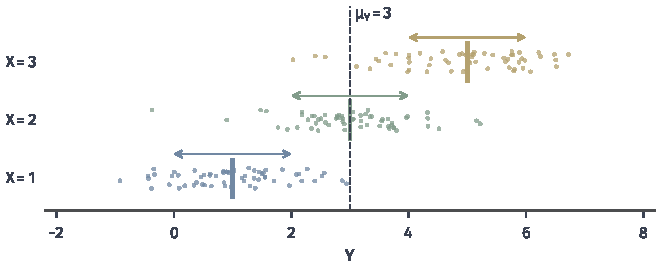
\includegraphics[width=112mm]{figures/01-basic-mathematics/05-probability-and-statistics-basics/matplotlib/rvec-total-variance/figure.pdf}
  \caption{全方差公式的组内与组间两部分。$X$等可能取$1,2,3$，给定$X=k$时$Y\sim\mathcal N(2k-1,1)$；每组画出$60$个模拟值（固定随机种子，纵向抖动只为避免重叠）。粗竖线是组均值，双箭头标出组均值左右各一个条件标准差，虚线是总均值$3$。组内方差为$1$，组间方差为$8/3$，总方差为$11/3$。}
  \label{fig:rvec-total-variance}
\end{figure}

对示例~\ref{ex:rvec-study-table}，组内部分为$0.3\times\frac29+0.4\times\frac{15}{64}+0.3\times\frac5{36}\approx0.2021$；组间部分为$0.3\times\frac19+0.4\times\frac{25}{64}+0.3\times\frac{25}{36}-0.6^2\approx0.0379$，两者之和恰为$0.24$。复习次数解释的只是考试结果总波动中约$16\%$的部分。两项都非负，所以$\mathbb E[\operatorname{Var}(Y\mid X)]\le\operatorname{Var}(Y)$：平均而言，获得信息不会增加波动。但在个别取值$x$上，条件方差可以大于无条件方差：若某门考试总体通过率为$0.9$，而其中一组学生的通过率只有$0.5$，这一组的条件方差$0.25$就大于总体方差$0.09$。

\subsection{条件独立}

\paragraph{定义}
条件分布也可以有独立结构。先固定第三个变量，再问两个变量是否独立，就得到条件独立。

\begin{definition}[条件独立]
设$(X,Y,Z)$是离散随机向量。若对所有满足$p_Z(z)>0$的$z$以及所有$x,y$，
\[
 p_{X,Y\mid Z}(x,y\mid z)=p_{X\mid Z}(x\mid z)\,p_{Y\mid Z}(y\mid z),
\]
则称在给定$Z$的条件下$X$与$Y$\term{条件独立}（conditionally independent），记为$X\perp Y\mid Z$。具有联合密度时，把质量函数换成相应的条件密度，在$f_Z(z)>0$处要求同样的分解。
\end{definition}

在相应条件分布有定义的位置，这个分解等价于$p_{X\mid Y,Z}(x\mid y,z)=p_{X\mid Z}(x\mid z)$：一旦知道$Z$，再得知$Y$不会改变$X$的条件分布。条件独立是对每个$z$分别检查的独立性，它与不加条件的独立是两种不同的要求。

\paragraph{共享参数造成的依赖}
设盒中有两枚外观相同的硬币，一枚正面概率为$0.2$，另一枚为$0.8$。随机取出一枚（各有概率$1/2$），记其正面概率为$\Theta$，再用它连抛两次，$X_1,X_2$表示两次是否正面。给定$\Theta=\theta$，两次抛掷独立，各以概率$\theta$正面朝上，所以$X_1\perp X_2\mid\Theta$。不知道是哪一枚硬币时，由全概率公式，
\[
\begin{aligned}
 \mathbb P(X_1=1)&=\tfrac12(0.2+0.8)=0.5,\\
 \mathbb P(X_1=1,X_2=1)&=\tfrac12(0.2^2+0.8^2)=0.34\neq0.5^2 .
\end{aligned}
\]
两次结果不独立：$\mathbb P(X_2=1\mid X_1=1)=0.34/0.5=0.68$。原因是第一次正面使“取到的是$0.8$那枚”更可信。由Bayes公式$\mathbb P(\Theta=0.8\mid X_1=1)=0.4/0.5=0.8$，再按全概率公式，第二次正面的概率为$0.8\times0.8+0.2\times0.2=0.68$，与上面一致。共享的未知参数使给定参数时独立的观测在边缘上产生依赖。

反方向也不成立。令$X,Y$独立，都等可能取$0$或$1$，$Z=X+Y$。给定$Z=1$时只剩$(1,0)$与$(0,1)$两种等可能结果，于是
$\mathbb P(X=1,Y=1\mid Z=1)=0$，而$\mathbb P(X=1\mid Z=1)\mathbb P(Y=1\mid Z=1)=1/4$。原本独立的两个变量，在得知它们的和以后变得完全相互决定。因此，条件独立和无条件独立不能互相推出，使用时必须说明以什么为条件。

\section{多个随机变量的组合与变换}
\label{sec:rvec-transforms}
\label{sec:rv-combinations}

第~\ref{sec:prob-univariate-transforms}节研究了一个随机变量经函数变换后的分布。多个变量时，我们关心的是和、乘积、比值以及线性组合等由几个分量共同决定的量。本节先把一元变量替换推广到向量，再用它处理和、乘积与比值，最后讨论仿射变换的均值与协方差。

\subsection{多元变量替换}

\paragraph{同维可逆变换的密度}
回顾一元情形：若$g$严格单调可微，$h=g^{-1}$，则$Y=g(X)$的密度为$f_Y(y)=f_X(h(y))\,|h'(y)|$，绝对导数因子补偿区间长度的伸缩。向量情形中，伸缩的是小块体积，第~\ref{sec:classical-change-variables}节已经说明，可微映射对体积的局部放大倍数是Jacobian行列式的绝对值。

\begin{theorem}[多元变量替换]
\label{thm:rvec-change-of-variables}
设$U,V\subseteq\mathbb R^d$为开集，随机向量$\bm X$的取值以概率$1$落在$U$中，并在$U$上具有连续的联合密度$f_{\bm X}$。设$g:U\to V$是双射，$g$与逆映射$h=g^{-1}$都连续可微。则$\bm Y=g(\bm X)$具有联合密度
\[
 f_{\bm Y}(\bm y)=f_{\bm X}\bigl(h(\bm y)\bigr)\,\bigl|\det\bm J_h(\bm y)\bigr|,\qquad\bm y\in V,
\]
在$V$外为零。其中$\bm J_h(\bm y)$是$h$在$\bm y$处的Jacobian矩阵，且$|\det\bm J_h(\bm y)|=1/|\det\bm J_g(h(\bm y))|$。
\end{theorem}

\begin{proof}
对$V$中的Jordan区域$B$，事件$\{\bm Y\in B\}$与$\{\bm X\in h(B)\}$相同，所以
\[
 \mathbb P(\bm Y\in B)=\int_{h(B)}f_{\bm X}(\bm x)\,\mathrm d\bm x=\int_Bf_{\bm X}\bigl(h(\bm y)\bigr)\bigl|\det\bm J_h(\bm y)\bigr|\,\mathrm d\bm y ,
\]
第二个等号是第~\ref{sec:classical-change-variables}节的区域积分换元公式，取那里的变换为$h$。右端被积函数给出$\bm Y$在每个区域上的概率，因而是$\bm Y$的联合密度。由$h(g(\bm x))=\bm x$及链式法则，$\bm J_h(g(\bm x))\bm J_g(\bm x)=\bm I$，取行列式得到最后一个等式。
\end{proof}

只把$\bm x=h(\bm y)$代入原密度而漏掉行列式因子，所得函数一般不能积分为$1$。行列式因子的含义是：$\bm y$附近体积为$\Delta V$的小块来自$\bm x$附近体积约为$|\det\bm J_h|\Delta V$的小块，两块的概率相同，所以密度要按体积比例换算。

\paragraph{计算步骤}
应用定理时，可以按四步组织：先确定$\bm X$的取值范围$U$及其像$V=g(U)$；再从$\bm y=g(\bm x)$解出逆映射$\bm x=h(\bm y)$；然后计算$\bm J_h$及其行列式的绝对值；最后写出$f_{\bm Y}$，并通过积分为$1$或已知的边缘分布检查结果。去掉一个概率为零的集合（例如一条射线）以满足双射条件，不影响任何概率。

\begin{example}[两个独立标准高斯变量的极坐标]
\label{ex:rvec-polar-gaussian}
设$X,Y$独立，都服从$\mathcal N(0,1)$，联合密度为$\frac1{2\pi}e^{-(x^2+y^2)/2}$。用极坐标表示点$(X,Y)$：$R=\sqrt{X^2+Y^2}$，$\Theta$为从正$x$轴量起的角度。去掉概率为零的射线$\{y=0,x\ge0\}$后，取$V=(0,\infty)\times(0,2\pi)$，逆映射为$h(r,\theta)=(r\cos\theta,r\sin\theta)$，其Jacobian行列式为$r$。于是
\[
 f_{R,\Theta}(r,\theta)=\frac1{2\pi}e^{-r^2/2}\cdot r=\bigl(re^{-r^2/2}\bigr)\cdot\frac1{2\pi},\qquad r>0,\ 0<\theta<2\pi .
\]
联合密度分解为$r$的函数与$\theta$的函数之积，取值范围也是乘积形状，所以$R\perp\Theta$，$\Theta\sim\operatorname{U}(0,2\pi)$，$R$的密度为$re^{-r^2/2}$。检查：$\int_0^\infty re^{-r^2/2}\,\mathrm dr=1$。进一步，$\mathbb P(R^2/2>t)=\mathbb P(R>\sqrt{2t})=\int_{\sqrt{2t}}^\infty re^{-r^2/2}\,\mathrm dr=e^{-t}$，即$R^2/2\sim\operatorname{Exp}(1)$。这个结论在第~\ref{sec:rvec-generation}节用于生成高斯变量。
\end{example}

\paragraph{维数改变的映射}
定理只适用于同维、可逆的映射。$S=X_1+X_2$把$\mathbb R^2$映到$\mathbb R$，Jacobian是$1\times2$矩阵，没有行列式可取。处理办法是补一个辅助变量，例如令$(U,S)=(X_1,X_1+X_2)$，得到同维可逆变换，算出联合密度后再对辅助变量积分，下面两小节都这样做。反方向的映射$X\mapsto(X,X)$把一维变量放进平面，像集中在一条直线上；直线面积为零，$(X,X)$没有二维联合密度，尽管两个分量各有一维密度。

\subsection{和的分布}

\paragraph{卷积公式}
两个变量之和是最常见的组合。离散情形，事件$\{X+Y=s\}$按$X$的取值拆开，
\[
 \mathbb P(X+Y=s)=\sum_xp_{X,Y}(x,s-x).
\]
连续情形按上一小节的方法，令$(U,S)=(X,X+Y)$。这是行列式为$1$的线性变换，逆映射为$(x,y)=(u,s-u)$，故$f_{U,S}(u,s)=f_{X,Y}(u,s-u)$。对辅助变量$u$积分，
\[
 f_{X+Y}(s)=\int f_{X,Y}(x,s-x)\,\mathrm dx .
\]
若$X\perp Y$，联合质量函数或联合密度分解为乘积，得到
\begin{equation}
 \mathbb P(X+Y=s)=\sum_xp_X(x)\,p_Y(s-x),\qquad
 f_{X+Y}(s)=\int f_X(x)\,f_Y(s-x)\,\mathrm dx .
 \label{eq:rvec-convolution}
\end{equation}
这种运算称为\term{卷积}（convolution）。它的含义是：和为$s$可以由“$X$取$x$、$Y$取$s-x$”的各种方式实现，把每种方式的概率（或密度）乘起来再汇总。

\begin{example}[两个独立均匀变量之和]
\label{ex:rvec-uniform-sum}
设$U_1,U_2$独立，都服从$\operatorname{U}(0,1)$。式~\eqref{eq:rvec-convolution}中被积函数在$0<x<1$且$0<s-x<1$时为$1$，其余为$0$，所以$f(s)$等于区间$(\max(0,s-1),\min(1,s))$的长度：
\[
 f_{U_1+U_2}(s)=\begin{cases}s,&0<s\le1,\\2-s,&1<s<2,\end{cases}
\]
其余为零。图~\ref{fig:rvec-convolution}(a)显示，两个均匀变量的和不再均匀，而是三角形：和接近$1$的组合方式最多，接近$0$或$2$时两个分量都必须接近端点。
\end{example}

\begin{figure}[htbp]
  \centering
  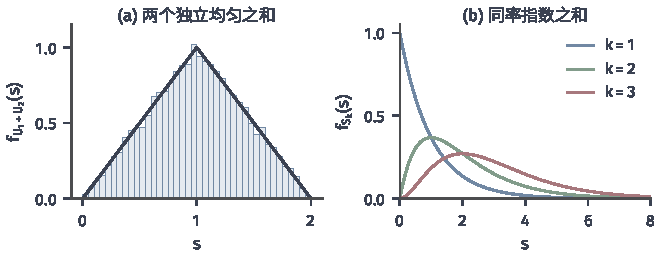
\includegraphics[width=112mm]{figures/01-basic-mathematics/05-probability-and-statistics-basics/matplotlib/rvec-convolution/figure.pdf}
  \caption{独立变量之和的密度。(a)两个独立$\operatorname{U}(0,1)$变量之和：直方图来自$20000$次模拟（固定随机种子），黑线是卷积得到的三角密度。(b)$k$个独立$\operatorname{Exp}(1)$变量之和$S_k$的密度$s^{k-1}e^{-s}/(k-1)!$，即$\operatorname{Gamma}(k,1)$；随$k$增大，峰值右移，分布变宽。}
  \label{fig:rvec-convolution}
\end{figure}

\paragraph{从Bernoulli到二项}
设$X_1,\ldots,X_n$相互独立，都服从$\operatorname{Bernoulli}(p)$，$S_n=X_1+\cdots+X_n$。对$n$归纳证明$S_n\sim\operatorname{Bin}(n,p)$。$n=1$时显然。设$S_{n-1}\sim\operatorname{Bin}(n-1,p)$；由分组独立的推论，$S_{n-1}\perp X_n$。按离散卷积，对$0\le k\le n$，
\[
\begin{aligned}
 \mathbb P(S_n=k)&=\mathbb P(S_{n-1}=k)(1-p)+\mathbb P(S_{n-1}=k-1)\,p\\
 &=\Bigl[\tbinom{n-1}{k}+\tbinom{n-1}{k-1}\Bigr]p^k(1-p)^{n-k}=\tbinom nkp^k(1-p)^{n-k},
\end{aligned}
\]
最后一步是组合数的Pascal递推，约定超出范围的组合数为零。这从卷积的角度重新得到了第~\ref{sec:prob-discrete-models}节的二项分布；独立与成功概率相同两个条件在递推的每一步都用到了。

\paragraph{从指数到Gamma}
第~\ref{sec:prob-gamma}节的$\operatorname{Gamma}(\alpha,\beta)$分布在$x>0$上的密度为$\frac{\beta^\alpha}{\Gamma(\alpha)}x^{\alpha-1}e^{-\beta x}$，$\alpha=1$时就是指数分布$\operatorname{Exp}(\beta)$。独立等待时间相加正好产生这一族分布。

\begin{theorem}[同率指数变量之和]
\label{thm:rvec-exponential-sum}
设$X_1,\ldots,X_k$相互独立，都服从$\operatorname{Exp}(\lambda)$。则$S_k=X_1+\cdots+X_k\sim\operatorname{Gamma}(k,\lambda)$，即
\[
 f_{S_k}(s)=\frac{\lambda^ks^{k-1}e^{-\lambda s}}{(k-1)!},\qquad s>0 .
\]
\end{theorem}

\begin{proof}
对$k$归纳。$k=1$时就是指数密度。设结论对$k-1$成立，$S_{k-1}\perp X_k$。两个变量都非负，卷积积分只在$0<x<s$上非零：
\[
\begin{aligned}
 f_{S_k}(s)&=\int_0^s\frac{\lambda^{k-1}x^{k-2}e^{-\lambda x}}{(k-2)!}\,\lambda e^{-\lambda(s-x)}\,\mathrm dx\\
 &=\lambda^ke^{-\lambda s}\int_0^s\frac{x^{k-2}}{(k-2)!}\,\mathrm dx=\frac{\lambda^ks^{k-1}e^{-\lambda s}}{(k-1)!} .
\end{aligned}
\]
两个指数因子合并后不再含$x$，这一步用到了两个率参数相同。
\end{proof}

例如某服务台两位顾客的服务时间独立，都服从$\operatorname{Exp}(2)$（单位：小时）。两位顾客的总服务时间超过$1$小时的概率为
\[
 \mathbb P(S_2>1)=\int_1^\infty4se^{-2s}\,\mathrm ds=3e^{-2}\approx0.406 ,
\]
而单独一位超过$1$小时的概率只有$e^{-2}\approx0.135$。图~\ref{fig:rvec-convolution}(b)画出了$\lambda=1$时$k=1,2,3$的密度。

定理的两个条件都不能省略。若率参数不同，$\lambda_1\neq\lambda_2$，同样的卷积给出$f(s)=\frac{\lambda_1\lambda_2}{\lambda_1-\lambda_2}(e^{-\lambda_2s}-e^{-\lambda_1s})$，不属于Gamma族。若不独立，例如两个“等待时间”其实是同一个$X\sim\operatorname{Exp}(\lambda)$，则$X+X=2X$满足$\mathbb P(2X>t)=e^{-\lambda t/2}$，服从$\operatorname{Exp}(\lambda/2)$，而不是$\operatorname{Gamma}(2,\lambda)$。

\subsection{乘积与比值的分布}

\paragraph{引入辅助变量}
乘积$XY$与比值$X/Y$同样是从二维到一维的映射，需要先补一个辅助变量。对乘积$W=XY$，在$x\neq0$的区域上令$(U,W)=(X,XY)$，逆映射为$(x,y)=(u,w/u)$，其Jacobian行列式为$1/u$。若$(X,Y)$有联合密度，则$\mathbb P(X=0)=0$，去掉这条直线不影响概率，于是
\[
 f_{XY}(w)=\int_{u\neq0}f_{X,Y}\Bigl(u,\frac wu\Bigr)\frac{\mathrm du}{|u|} .
\]
对比值$R=X/Y$，先检查分母：必须有$\mathbb P(Y=0)=0$，否则比值在正概率事件上没有定义。令$(R,V)=(X/Y,Y)$，逆映射为$(x,y)=(rv,v)$，行列式为$v$，得到
\[
 f_{X/Y}(r)=\int f_{X,Y}(rv,v)\,|v|\,\mathrm dv .
\]

\begin{example}[两个均匀变量的乘积]
\label{ex:rvec-uniform-product}
设$X,Y$独立，都服从$\operatorname{U}(0,1)$。被积函数在$0<u<1$且$0<w/u<1$即$w<u<1$时为$1$，故
\[
 f_{XY}(w)=\int_w^1\frac{\mathrm du}u=-\ln w,\qquad 0<w<1 .
\]
检查：$\int_0^1(-\ln w)\,\mathrm dw=1$。由此$\mathbb P(XY\le\frac12)=\int_0^{1/2}(-\ln w)\,\mathrm dw=\frac12+\frac12\ln2\approx0.847$。直接计算补事件也得到同样结果：$\mathbb P(XY>\frac12)=\int_{1/2}^1\bigl(1-\frac1{2x}\bigr)\mathrm dx=\frac12-\frac12\ln2$。
\end{example}

比值的分母可以取到零附近时，结果可能有很重的尾部。设$X,Y$独立，都服从$\mathcal N(0,1)$，则
\[
 f_{X/Y}(r)=\frac1{2\pi}\int_{-\infty}^{\infty}|v|e^{-(1+r^2)v^2/2}\,\mathrm dv=\frac1{\pi(1+r^2)} ,
\]
其中用到$\int_{-\infty}^\infty|v|e^{-av^2/2}\,\mathrm dv=2/a$。这是标准Cauchy分布。由于$\int|r|/(\pi(1+r^2))\,\mathrm dr$发散，比值的期望不存在，尽管分子和分母的各阶矩都有限。

\paragraph{由Gamma变量构造Beta变量}
第~\ref{sec:prob-beta}节的$\operatorname{Beta}(a,b)$分布在$(0,1)$上的密度为$t^{a-1}(1-t)^{b-1}/B(a,b)$，其中$B(a,b)=\int_0^1t^{a-1}(1-t)^{b-1}\,\mathrm dt$。它描述随机的比例。两段独立等待时间中第一段所占的比例，正好产生这一分布。

\begin{theorem}[Gamma变量的和与比例]
\label{thm:rvec-gamma-beta}
设$X\sim\operatorname{Gamma}(a,\beta)$，$Y\sim\operatorname{Gamma}(b,\beta)$，二者独立，率参数相同。令$S=X+Y$，$T=X/(X+Y)$。则$S\perp T$，且
\[
 S\sim\operatorname{Gamma}(a+b,\beta),\qquad T\sim\operatorname{Beta}(a,b).
\]
同时得到$B(a,b)=\Gamma(a)\Gamma(b)/\Gamma(a+b)$。
\end{theorem}

\begin{proof}
映射$(x,y)\mapsto(s,t)=(x+y,\,x/(x+y))$把$(0,\infty)^2$一一映到$(0,\infty)\times(0,1)$，逆映射为$(x,y)=(st,\,s(1-t))$，其Jacobian行列式为
\[
 \det\begin{bmatrix}t&s\\1-t&-s\end{bmatrix}=-ts-s(1-t)=-s .
\]
由独立性与定理~\ref{thm:rvec-change-of-variables}，
\[
\begin{aligned}
 f_{S,T}(s,t)&=\frac{\beta^a(st)^{a-1}e^{-\beta st}}{\Gamma(a)}\cdot\frac{\beta^b\bigl(s(1-t)\bigr)^{b-1}e^{-\beta s(1-t)}}{\Gamma(b)}\cdot s\\
 &=\frac{\beta^{a+b}s^{a+b-1}e^{-\beta s}}{\Gamma(a)\Gamma(b)}\cdot t^{a-1}(1-t)^{b-1}.
\end{aligned}
\]
两个指数因子$e^{-\beta st}e^{-\beta s(1-t)}=e^{-\beta s}$合并后不含$t$，这里用到了率参数相同。联合密度分解为$s$的函数与$t$的函数之积，取值范围是乘积形状，所以$S\perp T$。对$s$积分，由$\int_0^\infty s^{a+b-1}e^{-\beta s}\,\mathrm ds=\Gamma(a+b)/\beta^{a+b}$，
\[
 f_T(t)=\frac{\Gamma(a+b)}{\Gamma(a)\Gamma(b)}\,t^{a-1}(1-t)^{b-1},\qquad 0<t<1 .
\]
它是密度，积分为$1$，与$\operatorname{Beta}$密度的归一化比较即得$B(a,b)=\Gamma(a)\Gamma(b)/\Gamma(a+b)$。对$t$积分则得到$S$的$\operatorname{Gamma}(a+b,\beta)$密度。
\end{proof}

取$a=b=1$，$X,Y$是两个独立的$\operatorname{Exp}(\beta)$等待时间，第一段在总时间中所占比例$T$服从$\operatorname{Beta}(1,1)=\operatorname{U}(0,1)$：比例在$(0,1)$上完全均匀，与总时长无关，也与$\beta$无关。又如$a=2$、$b=3$时，$T\sim\operatorname{Beta}(2,3)$，均值为$2/5$。定理还顺带给出$S$的分布：同率独立Gamma变量之和仍是Gamma变量，形状参数相加，定理~\ref{thm:rvec-exponential-sum}是它的特例。若两个率参数不同，指数因子无法合并，$T$一般不再服从Beta分布。

\subsection{仿射变换与白化}
\label{sec:rvec-affine-whitening}

\paragraph{均值与协方差的变换}
许多组合量是分量的线性组合：多个读数的平均、两个读数之差、坐标的旋转与缩放。对这类变换，均值与协方差有简单的计算公式，不需要先求出完整分布。对两个随机向量，定义它们的\term{交叉协方差矩阵}（cross-covariance matrix）$\operatorname{Cov}(\bm X,\bm Y)=\mathbb E[(\bm X-\mathbb E\bm X)(\bm Y-\mathbb E\bm Y)^{\top}]$，其$(i,j)$元为$\operatorname{Cov}(X_i,Y_j)$。

\begin{theorem}[仿射变换的均值与协方差]
\label{thm:rvec-affine-moments}
设$\bm X\in\mathbb R^d$的均值为$\bm\mu$、协方差矩阵为$\bm\Sigma$，$\bm A\in\mathbb R^{m\times d}$，$\bm B\in\mathbb R^{k\times d}$，$\bm b\in\mathbb R^m$。则$\bm Y=\bm A\bm X+\bm b$满足
\[
 \mathbb E\bm Y=\bm A\bm\mu+\bm b,\qquad \operatorname{Cov}(\bm Y)=\bm A\bm\Sigma\bm A^{\top},\qquad
 \operatorname{Cov}(\bm A\bm X,\bm B\bm X)=\bm A\bm\Sigma\bm B^{\top}.
\]
\end{theorem}

\begin{proof}
均值公式已在第~\ref{sec:rvec-moments}节得到。由此$\bm Y-\mathbb E\bm Y=\bm A(\bm X-\bm\mu)$，故
\[
 (\bm Y-\mathbb E\bm Y)(\bm Y-\mathbb E\bm Y)^{\top}=\bm A(\bm X-\bm\mu)(\bm X-\bm\mu)^{\top}\bm A^{\top}.
\]
右端每个元素是$(\bm X-\bm\mu)(\bm X-\bm\mu)^{\top}$各元素的固定线性组合，逐元素取期望即得$\bm A\bm\Sigma\bm A^{\top}$。交叉协方差同理。
\end{proof}

公式对任意$m\times d$矩阵成立，不要求方阵，也不要求分布有密度。例如$m=1$、$\bm A=(1,1)$给出和的方差，与式~\eqref{eq:rvec-variance-of-combination}一致。求密度时则须检查维数与秩：$m=d$且$\bm A$可逆时，由定理~\ref{thm:rvec-change-of-variables}，$f_{\bm Y}(\bm y)=f_{\bm X}\bigl(\bm A^{-1}(\bm y-\bm b)\bigr)/|\det\bm A|$；$m<d$时需要补辅助变量再边缘化；$\bm A$的秩小于$m$时，$\operatorname{Cov}(\bm Y)$的秩不超过$\operatorname{rank}\bm A<m$，由第~\ref{sec:rvec-covariance-matrix}节，$\bm Y$集中在一个低维仿射子空间上，没有$m$维密度。

\begin{example}[和与差]
\label{ex:rvec-sum-difference}
设$\operatorname{Var}(X_1)=\operatorname{Var}(X_2)=1$，$\operatorname{Cov}(X_1,X_2)=0.5$。取$\bm A=\begin{bmatrix}1&1\\1&-1\end{bmatrix}$，即计算和与差：
\[
 \bm A\bm\Sigma\bm A^{\top}=\begin{bmatrix}1.5&1.5\\0.5&-0.5\end{bmatrix}\begin{bmatrix}1&1\\1&-1\end{bmatrix}=\begin{bmatrix}3&0\\0&1\end{bmatrix}.
\]
和的方差为$3$，差的方差为$1$，二者不相关。正相关使和的波动变大、差的波动变小。
\end{example}

\paragraph{白化}
上例中一个线性变换把相关的分量变成了不相关的分量。更进一步，能否找到线性变换，使结果的协方差矩阵恰好是单位矩阵？设$\bm\Sigma$正定。若矩阵$\bm W$满足$\bm W\bm\Sigma\bm W^{\top}=\bm I$，则
\[
 \bm Z=\bm W(\bm X-\bm\mu)
\]
的均值为零、协方差为$\bm I$：各分量方差为$1$，两两不相关。这样的操作称为\term{白化}（whitening）。

有两种常用的构造。第一种用Cholesky分解（式~\eqref{eq:matrix-analysis-cholesky}）$\bm\Sigma=\bm L\bm L^{\top}$，取$\bm W=\bm L^{-1}$，则$\bm L^{-1}\bm L\bm L^{\top}\bm L^{-\top}=\bm I$。第二种用谱分解（定理~\ref{thm:ls-real-symmetric-spectral}）$\bm\Sigma=\bm Q\bm\Lambda\bm Q^{\top}$，取对称平方根的逆$\bm W=\bm\Sigma^{-1/2}=\bm Q\bm\Lambda^{-1/2}\bm Q^{\top}$，矩阵平方根的计算见示例~\ref{ex:ls-matrix-square-root-two-by-two}。白化矩阵不唯一：若$\bm Z$已白化，$\bm O$是任意正交矩阵，则$\operatorname{Cov}(\bm O\bm Z)=\bm O\bm I\bm O^{\top}=\bm I$，旋转后的结果同样是白化的。

\begin{example}[用Cholesky因子白化]
\label{ex:rvec-whitening}
设$\bm\mu=(1,2)^{\top}$，$\bm\Sigma=\begin{bmatrix}4&2\\2&2\end{bmatrix}$。Cholesky因子为$\bm L=\begin{bmatrix}2&0\\1&1\end{bmatrix}$，可直接验证$\bm L\bm L^{\top}=\bm\Sigma$；其逆为$\bm L^{-1}=\begin{bmatrix}1/2&0\\-1/2&1\end{bmatrix}$。于是
\[
 Z_1=\frac{X_1-1}2,\qquad Z_2=(X_2-2)-\frac{X_1-1}2 .
\]
$Z_1$是标准化的第一个分量；$Z_2$从第二个分量中扣除了能由第一个分量线性说明的部分。验证：$\operatorname{Var}(Z_2)=2+\frac14\times4-2\times\frac12\times2=1$，$\operatorname{Cov}(Z_1,Z_2)=\frac12\times2-\frac14\times4=0$。
\end{example}

白化只保证不相关，不保证独立。图~\ref{fig:rvec-whitening}(c)中，原始样本由正方形上的均匀分布经线性变换得到，白化后协方差确实是$\bm I$，但样本均匀铺满一个倾斜的正方形：$z_1$接近正方形的左右顶点时，$z_2$只能取很窄的一段值，两个分量显然不独立。作为对照，同一协方差的高斯样本白化后，如图(b)所示呈圆形对称；第~\ref{sec:rvec-gaussian}节将说明，对联合高斯向量，白化后的分量确实相互独立。

\begin{figure}[htbp]
  \centering
  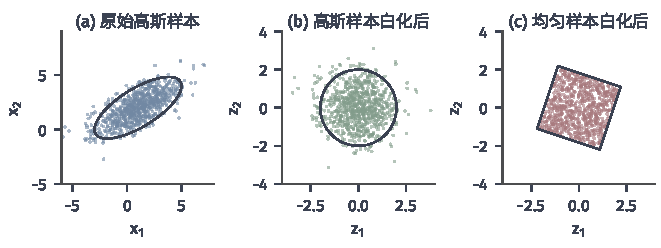
\includegraphics[width=112mm]{figures/01-basic-mathematics/05-probability-and-statistics-basics/matplotlib/rvec-whitening/figure.pdf}
  \caption{白化前后的样本，每幅$800$个模拟点（固定随机种子）。(a)均值与协方差同示例~\ref{ex:rvec-whitening}的高斯样本，椭圆是马氏距离为$2$的等密度线。(b)用Cholesky因子作变换$\bm z=\bm L^{-1}(\bm x-\bm\mu)$后，样本呈圆形对称。(c)同一协方差的非高斯样本（正方形上的均匀分布经线性变换得到）白化后，协方差同样是单位矩阵，但样本铺满一个倾斜的正方形，两个分量并不独立。}
  \label{fig:rvec-whitening}
\end{figure}

\section{随机变量的生成}
\label{sec:rvec-generation}
\label{sec:rv-random-generation}

上一节从已知分布出发计算变换后的分布。本节把问题方向转过来：给定目标分布，寻找能够产生它的随机输入和操作。模拟实验、随机算法和对模型的检验都需要这种能力。我们以第~\ref{sec:prob-continuous-models}节的标准均匀变量$U\sim\operatorname{U}(0,1)$为基本输入；计算机中的伪随机数生成器提供近似独立的均匀数，本书把它作为给定的工具。一元变量用逆变换生成，多元变量则按条件分解逐个生成；混合分布与随机参数模型是条件生成的两类具体应用。

\subsection{逆变换采样}

\paragraph{广义逆与生成定理}
第~\ref{sec:prob-numerical-features}节用分布函数的广义逆定义了分位数。对$0<u<1$，记
\[
 F^{-1}(u)=\inf\{x:F(x)\ge u\}.
\]
分布函数严格递增且连续时，它就是普通的反函数；有跳跃或平坦段时，下确界仍有定义。生成的思路是：把均匀分布的“累计概率”$u$通过分位数映回取值。

\begin{theorem}[逆变换采样]
\label{thm:rvec-inverse-transform}
设$F$是一个分布函数，$U\sim\operatorname{U}(0,1)$。则$X=F^{-1}(U)$的分布函数为$F$。
\end{theorem}

\begin{proof}
先证明：对$0<u<1$与实数$x$，$F^{-1}(u)\le x$当且仅当$u\le F(x)$。若$u\le F(x)$，则$x$属于定义下确界的集合，故$F^{-1}(u)\le x$。反过来，取该集合中趋于$F^{-1}(u)$的递减数列$x_n$，有$F(x_n)\ge u$；由分布函数的右连续性，$F\bigl(F^{-1}(u)\bigr)\ge u$。若$F^{-1}(u)\le x$，由单调性$F(x)\ge F\bigl(F^{-1}(u)\bigr)\ge u$。于是
\[
 \mathbb P(X\le x)=\mathbb P\bigl(F^{-1}(U)\le x\bigr)=\mathbb P\bigl(U\le F(x)\bigr)=F(x).
\]
\end{proof}

这种方法称为\term{逆变换采样}（inverse transform sampling）。图~\ref{fig:rvec-inverse-transform}给出了它的几何读法：在纵轴上取均匀点$u$，向右作水平线，碰到分布函数图像（或跳跃的竖直缺口）后向下投影，落点就是生成值。分布函数陡峭的地方，一段纵轴高度只对应很短的横轴区间，生成值在那里密集；平坦的地方则相反。

\begin{figure}[htbp]
  \centering
  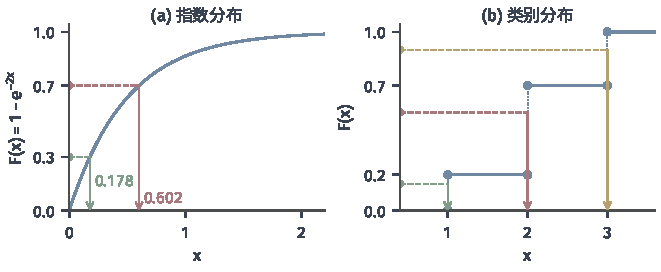
\includegraphics[width=112mm]{figures/01-basic-mathematics/05-probability-and-statistics-basics/matplotlib/rvec-inverse-transform/figure.pdf}
  \caption{逆变换采样的几何读法。(a)指数分布$\operatorname{Exp}(2)$：纵轴上的$u=0.3$和$u=0.7$经分布函数映回$x\approx0.178$和$x\approx0.602$。(b)在$1,2,3$上概率为$0.2,0.5,0.3$的类别分布：分布函数是阶梯，纵轴区间$(0,0.2]$、$(0.2,0.7]$、$(0.7,1]$分别映到$1$、$2$、$3$，图中$u=0.15,0.55,0.9$各落入一个区间。}
  \label{fig:rvec-inverse-transform}
\end{figure}

\paragraph{离散与连续两个例子}
定理不要求分布函数连续或严格递增，所以离散分布同样适用。设$X$在$\{1,2,3\}$上的概率为$0.2,0.5,0.3$，累计值为$c_1=0.2$、$c_2=0.7$、$c_3=1$。广义逆在$(0,0.2]$上取$1$，在$(0.2,0.7]$上取$2$，在$(0.7,1)$上取$3$，于是生成规则是“$U$落入第$k$段就输出$k$”，第$k$段的长度恰为$\pi_k$。分布函数的每一次跳跃把一整段$u$映到同一个取值；分布函数的平坦段（例如$1$与$2$之间）对应概率为零的区间，不会被生成。

对指数分布$\operatorname{Exp}(\lambda)$，$F(x)=1-e^{-\lambda x}$在$x>0$上连续递增，解$1-e^{-\lambda x}=u$得
\[
 F^{-1}(u)=-\frac{\ln(1-u)}\lambda .
\]
$\lambda=2$时，$u=0.3$生成$-\ln0.7/2\approx0.178$，$u=0.7$生成$-\ln0.3/2\approx0.602$。由于$1-U$与$U$同分布，也可以直接用$-\ln U/\lambda$。

\paragraph{用组合变换生成高斯变量}
逆变换采样需要能计算$F^{-1}$。标准高斯分布函数$\Phi$没有初等形式的反函数，此时可以把第~\ref{sec:rvec-transforms}节的变换倒过来使用。

\begin{example}[Box--Muller方法]
\label{ex:rvec-box-muller}
取独立的$U_1,U_2\sim\operatorname{U}(0,1)$，令
\[
 R=\sqrt{-2\ln U_1},\qquad \Theta=2\pi U_2,\qquad (X,Y)=(R\cos\Theta,\,R\sin\Theta).
\]
由逆变换采样，$-\ln U_1\sim\operatorname{Exp}(1)$，所以$R^2/2\sim\operatorname{Exp}(1)$，$R$的密度为$re^{-r^2/2}$；$\Theta\sim\operatorname{U}(0,2\pi)$且与$R$独立。这正是示例~\ref{ex:rvec-polar-gaussian}中$(R,\Theta)$的联合分布。把那里的极坐标变换反过来用一次定理~\ref{thm:rvec-change-of-variables}，即知$X,Y$是两个独立的标准高斯变量。
\end{example}

\subsection{条件生成}

\paragraph{按条件分解逐个生成}
多元变量可以拆成一连串一元问题。第~\ref{sec:rvec-conditioning}节的乘积关系$p_{X,Y}(x,y)=p_X(x)\,p_{Y\mid X}(y\mid x)$提示了生成顺序：先按$p_X$生成$X$，得到取值$x$以后，再用新的、独立的随机输入按条件分布$p_{Y\mid X}(\cdot\mid x)$生成$Y$。这样得到的一对$(X,Y)$满足
\[
\begin{aligned}
 \mathbb P(X=x,Y=y)&=\mathbb P(X=x)\,\mathbb P(Y=y\mid X=x)\\
 &=p_X(x)\,p_{Y\mid X}(y\mid x)=p_{X,Y}(x,y),
\end{aligned}
\]
恰好是目标联合分布；密度情形同理。$d$个变量时，反复使用乘法公式得到
\[
 p(x_1,\ldots,x_d)=p(x_1)\,p(x_2\mid x_1)\cdots p(x_d\mid x_1,\ldots,x_{d-1}),
\]
按这个顺序逐个生成即可。例如示例~\ref{ex:rvec-study-table}的概率表可以这样生成：先以概率$0.3,0.4,0.3$抽取$X\in\{0,1,2\}$，再按$\operatorname{Bernoulli}(m(X))$抽取$Y$，其中$m=(1/3,5/8,5/6)$。核对一格：$\mathbb P(X=2,Y=1)=0.3\times5/6=0.25$。

\paragraph{有限混合}
若观测来自几个未加标记的来源，例如两条产线的产品混在一起，可以先抽取来源标签，再按该来源的分布生成观测。设$Z\sim\operatorname{Cat}(\bm w)$取值$1,\ldots,K$，权重$w_k>0$且和为$1$；给定$Z=k$时，$X$的密度为$f_k$。由全概率公式，$\mathbb P(X\le x)=\sum_kw_k\,\mathbb P(X\le x\mid Z=k)$，求导得到
\[
 f_X(x)=\sum_{k=1}^Kw_kf_k(x).
\]
这样的分布称为\term{混合分布}（mixture distribution）。标签$Z$在观测中不出现，是一个\term{潜变量}（latent variable）；它不必对应真实可辨认的类别，主要用于组织模型与计算。

\begin{example}[两个高斯分量的混合]
\label{ex:rvec-gaussian-mixture}
取$\bm w=(1/4,3/4)$，$X\mid Z=1\sim\mathcal N(-1,1)$，$X\mid Z=2\sim\mathcal N(1,1)$。由全期望公式，$\mathbb EX=\frac14\times(-1)+\frac34\times1=\frac12$。由全方差公式，组内部分为$1$，组间部分为$\frac14\times1+\frac34\times1-\frac14=\frac34$，所以$\operatorname{Var}(X)=\frac74$；只平均两个分量的方差会漏掉均值不同造成的$3/4$。图~\ref{fig:rvec-gaussian-mixture}比较了两步生成的样本与混合密度：密度只有一个峰，但左侧明显比单个高斯更厚，这是权重较小的左分量的贡献。
\end{example}

\begin{figure}[htbp]
  \centering
  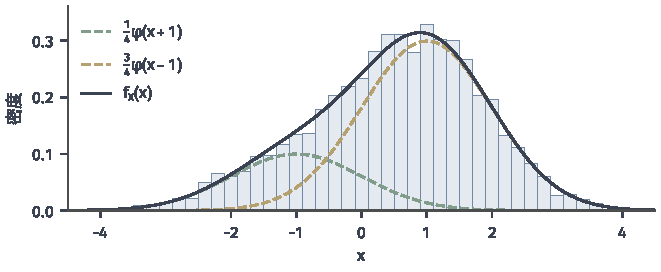
\includegraphics[width=112mm]{figures/01-basic-mathematics/05-probability-and-statistics-basics/matplotlib/rvec-mixture/figure.pdf}
  \caption{两个高斯分量的混合。先以概率$1/4,3/4$抽取标签，再从$\mathcal N(-1,1)$或$\mathcal N(1,1)$生成观测；直方图来自$4000$次两步生成（固定随机种子）。两条虚线是加权后的分量密度，黑线是它们的和$f_X$，其中$\varphi$为标准高斯密度。}
  \label{fig:rvec-gaussian-mixture}
\end{figure}

反过来，观测到$X=x$以后，可以用Bayes公式推断它来自哪个分量：
\[
 \mathbb P(Z=k\mid X=x)=\frac{w_kf_k(x)}{\sum_jw_jf_j(x)} .
\]
这里条件变量$Z$离散、观测$X$有密度，公式可以像条件密度那样由窄带$\{x\le X\le x+h\}$上的条件概率取极限得到。在上例中，$x=0$处两个分量密度相等，后验概率就等于权重$(1/4,3/4)$；$x=1$处，$\mathbb P(Z=1\mid X=1)=\frac{\frac14e^{-2}}{\frac14e^{-2}+\frac34}\approx0.043$。

\paragraph{随机参数模型}
另一类常见的条件生成是先生成参数，再在参数给定时生成多个观测。设参数$\Theta$有密度$f_\Theta$，给定$\Theta=\theta$时，$X_1,\ldots,X_n$条件独立，各自服从由$\theta$决定的同一分布$p(\cdot\mid\theta)$。联合分布为
\[
 f_\Theta(\theta)\prod_{i=1}^np(x_i\mid\theta),
\]
生成时先抽$\Theta$，再用这个取值独立地抽出$n$个观测。这样的分层构造称为\term{层次模型}（hierarchical model）。第~\ref{sec:rvec-conditioning}节的两枚硬币例子是参数只取两个值的情形；下面让参数在$(0,1)$上连续变化。

\begin{example}[Beta--Bernoulli模型]
\label{ex:rvec-beta-bernoulli}
设$\Theta\sim\operatorname{Beta}(a,b)$，给定$\Theta=\theta$时$X_1,\ldots,X_n$条件独立，都服从$\operatorname{Bernoulli}(\theta)$。可以把$\Theta$理解为某个未知的成功率，$X_i$为各次试验的结果。对观测序列$x_1,\ldots,x_n\in\{0,1\}$，记成功次数$k=\sum_ix_i$。把全概率公式中的求和换成对参数的积分，
\[
\begin{aligned}
 \mathbb P(X_1=x_1,\ldots,X_n=x_n)&=\int_0^1\theta^k(1-\theta)^{n-k}\frac{\theta^{a-1}(1-\theta)^{b-1}}{B(a,b)}\,\mathrm d\theta\\
 &=\frac{B(a+k,\,b+n-k)}{B(a,b)} .
\end{aligned}
\]
它只依赖成功次数$k$，不依赖成功出现的顺序。

用条件期望计算依赖强度更直接。给定$\Theta$，$\mathbb E[X_1\mid\Theta]=\Theta$；由条件独立，$\mathbb E[X_1X_2\mid\Theta]=\Theta^2$。由全期望公式，
\[
\begin{gathered}
 \mathbb P(X_1=1)=\mathbb E\Theta,\qquad \mathbb E[X_1X_2]=\mathbb E\Theta^2,\\
 \operatorname{Cov}(X_1,X_2)=\mathbb E\Theta^2-(\mathbb E\Theta)^2=\operatorname{Var}(\Theta)>0 .
\end{gathered}
\]
由第~\ref{sec:prob-beta}节，$\mathbb E\Theta=a/(a+b)$，$\operatorname{Var}(\Theta)=ab/\bigl((a+b)^2(a+b+1)\bigr)$。又$\operatorname{Var}(X_1)=\mathbb E\Theta(1-\mathbb E\Theta)=ab/(a+b)^2$，所以
\[
 \operatorname{Corr}(X_1,X_2)=\frac1{a+b+1} .
\]
$a=b=1$时$\Theta$在$(0,1)$上均匀，$\mathbb P(X_1=1)=1/2$，$\mathbb P(X_1=1,X_2=1)=\mathbb E\Theta^2=1/3$，于是$\mathbb P(X_2=1\mid X_1=1)=2/3$，相关系数为$1/3$。$a=b=10$时$\Theta$集中在$1/2$附近，相关系数降为$1/21\approx0.048$。
\end{example}

这个例子说明了共享参数产生依赖的机制：给定参数时观测条件独立，但参数未知时，每个观测都携带关于参数的信息，进而影响对其他观测的预测。参数越不确定（$\operatorname{Var}(\Theta)$越大），观测之间的边缘依赖越强；参数完全确定时，依赖消失。由观测更新$\Theta$的分布是第~\ref{sec:est-posterior}节的后验计算，据此预测下一次结果则在第~\ref{sec:pred-prediction}节讨论；本节只关心模型怎样生成数据以及由此产生的依赖结构。

\section{多元高斯分布}
\label{sec:rvec-gaussian}

前面各节分别建立了联合与边缘分布、协方差、独立与条件分布、变换与生成。本节集中研究一个模型，在其中把这些操作全部做一遍。多元高斯分布由均值向量和协方差矩阵完全确定，上述每一种操作都能在这两个参数上直接完成。

\subsection{多元高斯分布的定义}

\paragraph{密度与等密度椭球}
第~\ref{sec:prob-gaussian}节的一元高斯密度在指数中含有$(x-\mu)^2/\sigma^2$，即偏离量按方差标准化后的平方。多元情形中偏离是一个向量，自然的推广是用协方差矩阵的逆构造二次型。

\begin{definition}[多元高斯分布]
设$\bm\mu\in\mathbb R^d$，$\bm\Sigma$是$d\times d$对称正定矩阵。若随机向量$\bm X$的联合密度为
\begin{equation}
 f_{\bm X}(\bm x)=\frac1{(2\pi)^{d/2}(\det\bm\Sigma)^{1/2}}
 \exp\Bigl\{-\frac12(\bm x-\bm\mu)^{\top}\bm\Sigma^{-1}(\bm x-\bm\mu)\Bigr\},\qquad\bm x\in\mathbb R^d,
 \label{eq:rvec-gaussian-density}
\end{equation}
则称$\bm X$服从参数为$\bm\mu,\bm\Sigma$的\term{多元高斯分布}（multivariate Gaussian distribution），记为$\bm X\sim\mathcal N(\bm\mu,\bm\Sigma)$。
\end{definition}

$d=1$时它回到一元高斯密度。下一小节将验证这个函数积分为$1$，且$\bm\mu$与$\bm\Sigma$正是$\bm X$的均值向量与协方差矩阵。若$\bm\Sigma$是对角矩阵，二次型分解为$\sum_i(x_i-\mu_i)^2/\sigma_i^2$，密度变成$d$个一元高斯密度之积，各分量相互独立。

密度只通过二次型$Q(\bm x)=(\bm x-\bm\mu)^{\top}\bm\Sigma^{-1}(\bm x-\bm\mu)$依赖$\bm x$，所以等密度集合是$Q(\bm x)=c^2$。用谱分解$\bm\Sigma=\sum_i\lambda_i\bm q_i\bm q_i^{\top}$，在以$\bm\mu$为原点、以特征向量$\bm q_i$为坐标轴的坐标$u_i=\bm q_i^{\top}(\bm x-\bm\mu)$下，$Q=\sum_iu_i^2/\lambda_i$。因此等密度集合是以$\bm\mu$为中心的椭球，主轴沿特征向量方向，半轴长为$c\sqrt{\lambda_i}$：方差大的方向上椭球更长。$\sqrt{Q(\bm x)}$称为$\bm x$到$\bm\mu$的\term{马氏距离}（Mahalanobis distance），它按各方向的波动大小度量偏离。

\begin{example}[一个二维高斯分布]
\label{ex:rvec-gaussian-2d}
本节始终使用示例~\ref{ex:rvec-whitening}的参数$\bm\mu=(1,2)^{\top}$，$\bm\Sigma=\begin{bmatrix}4&2\\2&2\end{bmatrix}$。此时$\det\bm\Sigma=4$，
\[
 \bm\Sigma^{-1}=\begin{bmatrix}1/2&-1/2\\-1/2&1\end{bmatrix},\qquad
 Q(\bm x)=\tfrac12u_1^2-u_1u_2+u_2^2,\quad \bm u=\bm x-\bm\mu .
\]
特征值为$3\pm\sqrt5$，约为$5.24$与$0.76$。长轴方向的特征向量满足$(4-\lambda)v_1+2v_2=0$，取$\lambda=3+\sqrt5$得斜率$v_2/v_1=(\sqrt5-1)/2\approx0.62$。图~\ref{fig:rvec-gaussian-conditional}(a)画出了$c=1,2,3$的等密度椭圆：它们向右上方倾斜，反映两个分量正相关，相关系数为$2/\sqrt{4\times2}\approx0.71$。
\end{example}

\paragraph{分量高斯不等于联合高斯}
联合高斯是整个向量的性质，不能由每个分量的分布判断。示例~\ref{ex:rvec-random-sign}的$(Z,SZ)$两个分量都服从$\mathcal N(0,1)$，但它们不是联合高斯：散点全部落在两条对角线上，面积为零，没有二维联合密度。下一小节将证明，联合高斯向量的任何非零线性组合都服从一元高斯分布；而$Z+SZ$在$S=-1$时等于零，$\mathbb P(Z+SZ=0)=1/2$，一个正方差的高斯变量取任何单点的概率都是零。因此，即使每个分量都是高斯变量，向量整体也可能不是多元高斯分布。

\subsection{仿射变换与生成}

\paragraph{由独立标准高斯变量生成}
最简单的多元高斯向量由独立的标准高斯变量排成。设$Z_1,\ldots,Z_d$相互独立，都服从$\mathcal N(0,1)$，则$\bm Z=(Z_1,\ldots,Z_d)^{\top}$的联合密度为
\[
 \prod_{i=1}^d\frac1{\sqrt{2\pi}}e^{-z_i^2/2}=\frac1{(2\pi)^{d/2}}e^{-\bm z^{\top}\bm z/2},
\]
正是式~\eqref{eq:rvec-gaussian-density}取$\bm\mu=\bm0$、$\bm\Sigma=\bm I$的情形，即$\bm Z\sim\mathcal N(\bm0,\bm I)$。一般的高斯向量可以由它经可逆仿射变换得到。

\begin{theorem}[多元高斯向量的生成]
\label{thm:rvec-gaussian-generation}
设$\bm Z\sim\mathcal N(\bm0,\bm I_d)$，$\bm A$是$d\times d$可逆矩阵，$\bm A\bm A^{\top}=\bm\Sigma$。则$\bm X=\bm\mu+\bm A\bm Z\sim\mathcal N(\bm\mu,\bm\Sigma)$。特别地，式~\eqref{eq:rvec-gaussian-density}积分为$1$，且$\mathbb E\bm X=\bm\mu$，$\operatorname{Cov}(\bm X)=\bm\Sigma$。
\end{theorem}

\begin{proof}
映射$\bm z\mapsto\bm\mu+\bm A\bm z$可逆，逆映射为$\bm z=\bm A^{-1}(\bm x-\bm\mu)$，其Jacobian行列式为$\det\bm A^{-1}$。由$\det\bm\Sigma=(\det\bm A)^2$，$|\det\bm A^{-1}|=(\det\bm\Sigma)^{-1/2}$。又
\[
 \bm z^{\top}\bm z=(\bm x-\bm\mu)^{\top}\bm A^{-\top}\bm A^{-1}(\bm x-\bm\mu)=(\bm x-\bm\mu)^{\top}\bm\Sigma^{-1}(\bm x-\bm\mu),
\]
因为$\bm A^{-\top}\bm A^{-1}=(\bm A\bm A^{\top})^{-1}$。代入定理~\ref{thm:rvec-change-of-variables}，$\bm X$的密度正是式~\eqref{eq:rvec-gaussian-density}。它是一个随机向量的密度，积分自然为$1$。由定理~\ref{thm:rvec-affine-moments}，$\mathbb E\bm X=\bm\mu$，$\operatorname{Cov}(\bm X)=\bm A\bm I\bm A^{\top}=\bm\Sigma$。
\end{proof}

满足$\bm A\bm A^{\top}=\bm\Sigma$的矩阵可取Cholesky因子$\bm L$，也可取对称平方根$\bm\Sigma^{1/2}$。于是生成$\mathcal N(\bm\mu,\bm\Sigma)$的步骤是：分解$\bm\Sigma=\bm L\bm L^{\top}$；生成$d$个独立标准高斯数组成$\bm z$（例如用Box--Muller方法）；输出$\bm x=\bm\mu+\bm L\bm z$。这正是白化的逆过程。对示例~\ref{ex:rvec-gaussian-2d}，$\bm L=\begin{bmatrix}2&0\\1&1\end{bmatrix}$，
\[
 X_1=1+2Z_1,\qquad X_2=2+Z_1+Z_2 .
\]
例如$\bm z=(0.5,-1)^{\top}$生成$\bm x=(2,1.5)^{\top}$。两个分量共享$Z_1$，这就是它们正相关的来源：$\operatorname{Cov}(X_1,X_2)=2\operatorname{Var}(Z_1)=2$。

\paragraph{仿射变换保持高斯结构}
高斯向量经过线性变换后仍是高斯向量，这是这一模型便于计算的根本原因。

\begin{theorem}[仿射变换]
\label{thm:rvec-gaussian-affine}
设$\bm X\sim\mathcal N(\bm\mu,\bm\Sigma)$，$\bm B$是秩为$m$的$m\times d$矩阵，$\bm c\in\mathbb R^m$。则
\[
 \bm B\bm X+\bm c\sim\mathcal N\bigl(\bm B\bm\mu+\bm c,\;\bm B\bm\Sigma\bm B^{\top}\bigr).
\]
特别地，对任意$\bm a\neq\bm0$，$\bm a^{\top}\bm X\sim\mathcal N(\bm a^{\top}\bm\mu,\bm a^{\top}\bm\Sigma\bm a)$。
\end{theorem}

\begin{proof}
由定理~\ref{thm:rvec-gaussian-generation}，可写$\bm X=\bm\mu+\bm L\bm Z$，于是$\bm B\bm X+\bm c=\bm B\bm\mu+\bm c+\bm M\bm Z$，其中$\bm M=\bm B\bm L$的秩为$m$，$\bm M\bm M^{\top}=\bm B\bm\Sigma\bm B^{\top}$正定。只需证明$\bm M\bm Z\sim\mathcal N(\bm0,\bm M\bm M^{\top})$。

令$\bm K=(\bm M\bm M^{\top})^{-1/2}\bm M$，其中逆平方根由谱分解给出。则$\bm K\bm K^{\top}=\bm I_m$，即$\bm K$的$m$行是标准正交的。用Gram--Schmidt正交化（第~\ref{chap:normed-inner-product-spaces}章）把这些行补成$\mathbb R^d$的标准正交基，排成正交矩阵$\bm O=\begin{bmatrix}\bm K\\\bm K'\end{bmatrix}$。由定理~\ref{thm:rvec-gaussian-generation}（取$\bm A=\bm O$，$\bm O\bm O^{\top}=\bm I$），$\bm O\bm Z\sim\mathcal N(\bm0,\bm I_d)$，即$\bm O\bm Z$的$d$个分量是独立的标准高斯变量。它的前$m$个分量$\bm K\bm Z$的联合密度由乘积密度对其余分量积分得到，各因子积分为$1$，所以$\bm K\bm Z\sim\mathcal N(\bm0,\bm I_m)$。最后$\bm M\bm Z=(\bm M\bm M^{\top})^{1/2}\bm K\bm Z$，再用一次定理~\ref{thm:rvec-gaussian-generation}即得结论。
\end{proof}

对示例~\ref{ex:rvec-gaussian-2d}，$X_1+X_2\sim\mathcal N(3,\,4+2\times2+2)=\mathcal N(3,10)$。又取$\bm a=(-1/2,1)^{\top}$，$\bm a^{\top}\bm\Sigma\bm a=\frac14\times4-2\times\frac12\times2+2=1$，故$X_2-X_1/2\sim\mathcal N(3/2,1)$；它减去均值就是示例~\ref{ex:rvec-whitening}中的$Z_2$。

\paragraph{退化高斯分布}
若矩阵的秩不足，结论需要修改。例如取$\bm B=\begin{bmatrix}1&1\\2&2\end{bmatrix}$，$\bm B\bm X=(S,2S)^{\top}$，其中$S=X_1+X_2\sim\mathcal N(3,10)$。这个二维向量全部落在直线$y=2x$上，没有二维密度，$\bm B\bm\Sigma\bm B^{\top}$也是奇异的。更一般地，对任意矩阵$\bm M$（不论秩），称$\bm c+\bm M\bm Z$的分布为（可能）\term{退化高斯分布}（degenerate Gaussian distribution），其均值为$\bm c$、协方差为$\bm M\bm M^{\top}$。秩不足时概率集中在仿射子空间$\bm c+\operatorname{range}(\bm M)$上，在这个子空间内的坐标下仍是非退化的高斯分布。这个分布只取决于$\bm c$与$\bm M\bm M^{\top}$，而不取决于$\bm M$本身的选取；证明需要特征函数，留到\BookPartRef{part:probability-spaces}{卷2《数学准备：抽象数学》的“概率空间”部分}。有了这一推广，定理~\ref{thm:rvec-gaussian-affine}对任意$\bm B$都成立，只是结果可能退化。

\subsection{边缘分布}

\paragraph{取出部分分量}
取出部分分量是一个特殊的线性映射。设$\bm X\sim\mathcal N(\bm\mu,\bm\Sigma)$，要保留前$k$个分量$\bm X_1=(X_1,\ldots,X_k)^{\top}$，取$\bm B=[\bm I_k\ \bm0]$，它的秩为$k$。由定理~\ref{thm:rvec-gaussian-affine}，
\[
 \bm X_1\sim\mathcal N(\bm\mu_1,\bm\Sigma_{11}),
\]
其中$\bm\mu_1$是$\bm\mu$的前$k$个分量，$\bm\Sigma_{11}$是$\bm\Sigma$左上角的$k\times k$子矩阵。保留任意一组分量时，选出$\bm I_d$的相应行即可。高斯分布的边缘化因此不需要计算积分，只需从参数中取出相应的子向量和子矩阵。示例~\ref{ex:rvec-gaussian-2d}中，$X_1\sim\mathcal N(1,4)$，$X_2\sim\mathcal N(2,2)$。

\paragraph{分块记号}
为了讨论两组分量之间的关系，把向量与参数按相同方式分块：
\[
 \bm X=\begin{bmatrix}\bm X_1\\\bm X_2\end{bmatrix},\qquad
 \bm\mu=\begin{bmatrix}\bm\mu_1\\\bm\mu_2\end{bmatrix},\qquad
 \bm\Sigma=\begin{bmatrix}\bm\Sigma_{11}&\bm\Sigma_{12}\\\bm\Sigma_{21}&\bm\Sigma_{22}\end{bmatrix},
\]
其中$\bm\Sigma_{12}=\operatorname{Cov}(\bm X_1,\bm X_2)$是两块之间的交叉协方差矩阵，$\bm\Sigma_{21}=\bm\Sigma_{12}^{\top}$。两个边缘分布只用到对角块$\bm\mu_1,\bm\Sigma_{11}$与$\bm\mu_2,\bm\Sigma_{22}$；两组分量之间的联系全部记录在$\bm\Sigma_{12}$中。例如把示例~\ref{ex:rvec-gaussian-2d}的非对角元由$2$改为$0$或$-1$，两个边缘分布不变，联合分布却不同。下面两小节分别回答：$\bm\Sigma_{12}=\bm0$意味着什么，以及观测到$\bm X_2$以后$\bm X_1$的分布怎样计算。

\subsection{独立性}

\paragraph{零交叉协方差推出独立}
第~\ref{sec:rvec-independence}节说明不相关一般推不出独立。联合高斯模型是一个重要例外。这里两个随机向量的独立按第~\ref{sec:rvec-independence}节的定义理解，只是把$A,B$换成相应维数空间中的集合；密度判定照样成立。

\begin{theorem}[联合高斯向量的分块独立]
\label{thm:rvec-gaussian-independence}
设$\bm X\sim\mathcal N(\bm\mu,\bm\Sigma)$按上述方式分块。若$\bm\Sigma_{12}=\bm0$，则$\bm X_1\perp\bm X_2$。
\end{theorem}

\begin{proof}
$\bm\Sigma_{12}=\bm0$时$\bm\Sigma$是分块对角矩阵，于是
\[
 \bm\Sigma^{-1}=\begin{bmatrix}\bm\Sigma_{11}^{-1}&\bm0\\\bm0&\bm\Sigma_{22}^{-1}\end{bmatrix},\qquad
 \det\bm\Sigma=\det\bm\Sigma_{11}\det\bm\Sigma_{22},
\]
二次型分成两项：$(\bm x-\bm\mu)^{\top}\bm\Sigma^{-1}(\bm x-\bm\mu)=(\bm x_1-\bm\mu_1)^{\top}\bm\Sigma_{11}^{-1}(\bm x_1-\bm\mu_1)+(\bm x_2-\bm\mu_2)^{\top}\bm\Sigma_{22}^{-1}(\bm x_2-\bm\mu_2)$。常数因子$(2\pi)^{d/2}$也按维数拆开。因此式~\eqref{eq:rvec-gaussian-density}等于$\mathcal N(\bm\mu_1,\bm\Sigma_{11})$与$\mathcal N(\bm\mu_2,\bm\Sigma_{22})$两个密度之积，而它们正是两块的边缘密度。由独立性的密度判定，$\bm X_1\perp\bm X_2$。
\end{proof}

逐个分量地应用：若$\bm\Sigma$是对角矩阵，联合高斯向量的各分量相互独立。定理的条件是整个向量联合高斯，而不只是各分量高斯。示例~\ref{ex:rvec-random-sign}中$\operatorname{Cov}(Z,SZ)=\mathbb E[S]\,\mathbb E[Z^2]=0$，两个分量都是标准高斯变量，却并不独立；它们不是联合高斯，定理不适用。

\paragraph{白化后的独立性}
回到第~\ref{sec:rvec-affine-whitening}节的白化。若$\bm X\sim\mathcal N(\bm\mu,\bm\Sigma)$，则由定理~\ref{thm:rvec-gaussian-affine}，$\bm Z=\bm L^{-1}(\bm X-\bm\mu)\sim\mathcal N(\bm0,\bm I)$。协方差为单位矩阵，由上面的定理，$\bm Z$的分量是相互独立的标准高斯变量。对一般分布，白化只能保证不相关；对联合高斯向量，白化把分量变成了独立变量，图~\ref{fig:rvec-whitening}(b)与(c)的差别正在于此。又因为$\mathcal N(\bm0,\bm I)$经任意正交变换仍是$\mathcal N(\bm0,\bm I)$，高斯情形下白化矩阵的不唯一性不影响这个结论。

\subsection{条件分布}
\label{sec:rvec-gaussian-conditioning}

\paragraph{条件均值与条件协方差}
观测到一部分分量以后，其余分量的分布应当怎样计算？对联合高斯向量，答案仍是高斯分布，参数可以由分块协方差直接写出。思路是把$\bm X_1$拆成“由$\bm X_2$线性决定的部分”与“和$\bm X_2$独立的残差”。

\begin{theorem}[高斯条件分布]
\label{thm:rvec-gaussian-conditional}
设$\bm X\sim\mathcal N(\bm\mu,\bm\Sigma)$按上述方式分块。对任意$\bm x_2$，
\begin{equation}
 \bm X_1\mid\bm X_2=\bm x_2\ \sim\ \mathcal N\Bigl(\bm\mu_1+\bm\Sigma_{12}\bm\Sigma_{22}^{-1}(\bm x_2-\bm\mu_2),\ \ \bm\Sigma_{11}-\bm\Sigma_{12}\bm\Sigma_{22}^{-1}\bm\Sigma_{21}\Bigr).
 \label{eq:rvec-gaussian-conditional}
\end{equation}
\end{theorem}

\begin{proof}
记$\bm K=\bm\Sigma_{12}\bm\Sigma_{22}^{-1}$（$\bm\Sigma_{22}$作为正定矩阵的主子矩阵是正定的，因而可逆），令残差
\[
 \bm R=\bm X_1-\bm\mu_1-\bm K(\bm X_2-\bm\mu_2).
\]
向量$(\bm R,\bm X_2)$由$\bm X$经可逆仿射变换得到，变换矩阵$\begin{bmatrix}\bm I&-\bm K\\\bm0&\bm I\end{bmatrix}$是行列式为$1$的分块三角矩阵，所以$(\bm R,\bm X_2)$联合高斯。由定理~\ref{thm:rvec-affine-moments}，
\[
\begin{aligned}
 \operatorname{Cov}(\bm R,\bm X_2)&=\bm\Sigma_{12}-\bm K\bm\Sigma_{22}=\bm0,\\
 \operatorname{Cov}(\bm R)&=\bm\Sigma_{11}-\bm K\bm\Sigma_{21}-\bm\Sigma_{12}\bm K^{\top}+\bm K\bm\Sigma_{22}\bm K^{\top}\\
 &=\bm\Sigma_{11}-\bm\Sigma_{12}\bm\Sigma_{22}^{-1}\bm\Sigma_{21},
\end{aligned}
\]
后一式中三项$\bm K\bm\Sigma_{21}$、$\bm\Sigma_{12}\bm K^{\top}$、$\bm K\bm\Sigma_{22}\bm K^{\top}$都等于$\bm\Sigma_{12}\bm\Sigma_{22}^{-1}\bm\Sigma_{21}$。记这个矩阵为$\bm S$。$(\bm R,\bm X_2)$的协方差矩阵是正定矩阵经可逆合同变换的结果，仍正定，所以其对角块$\bm S$正定。由定理~\ref{thm:rvec-gaussian-independence}，$\bm R\perp\bm X_2$，且$\bm R\sim\mathcal N(\bm0,\bm S)$。

记$m(\bm x_2)=\bm\mu_1+\bm K(\bm x_2-\bm\mu_2)$。对$(\bm x_1,\bm x_2)\mapsto(\bm x_1-m(\bm x_2),\bm x_2)$用定理~\ref{thm:rvec-change-of-variables}（行列式为$1$），并利用独立性，
\[
 f_{\bm X_1,\bm X_2}(\bm x_1,\bm x_2)=f_{\bm R,\bm X_2}\bigl(\bm x_1-m(\bm x_2),\bm x_2\bigr)=f_{\bm R}\bigl(\bm x_1-m(\bm x_2)\bigr)f_{\bm X_2}(\bm x_2).
\]
除以$f_{\bm X_2}(\bm x_2)>0$，条件密度为$f_{\bm R}\bigl(\bm x_1-m(\bm x_2)\bigr)$，即$\mathcal N\bigl(m(\bm x_2),\bm S\bigr)$的密度。
\end{proof}

条件协方差$\bm S=\bm\Sigma_{11}-\bm\Sigma_{12}\bm\Sigma_{22}^{-1}\bm\Sigma_{21}$正是$\bm\Sigma$中对块$\bm\Sigma_{22}$的Schur补；式~\eqref{eq:matrix-analysis-schur-positive-definite}说明了它为何正定。从协方差的角度看，它是从$\bm X_1$的原有波动$\bm\Sigma_{11}$中扣除能由$\bm X_2$线性说明的部分后剩下的波动。对联合密度的指数直接配方，借助分块逆公式~\eqref{eq:matrix-analysis-block-inverse}，也能得到同样的结果；上面的残差证明则说明了结果的含义。条件均值是$\bm x_2$的仿射函数，条件协方差则完全不依赖观测值$\bm x_2$：残差与$\bm X_2$独立，观测只移动中心，不改变围绕中心的波动。

\paragraph{二维算例}
对示例~\ref{ex:rvec-gaussian-2d}，以$X_1$为观测分量、求$X_2$的条件分布，把公式中两块的角色互换：
\[
\begin{aligned}
 \mathbb E[X_2\mid X_1=x_1]&=2+\frac24(x_1-1)=2+\frac{x_1-1}2,\\
 \operatorname{Var}(X_2\mid X_1=x_1)&=2-\frac{2\times2}4=1 .
\end{aligned}
\]
观测到$X_1=5$时，$X_2\mid X_1=5\sim\mathcal N(4,1)$。观测之前，$X_2\sim\mathcal N(2,2)$，$\mathbb P(X_2>3)=1-\Phi(1/\sqrt2)\approx0.240$；观测之后，$\mathbb P(X_2>3\mid X_1=5)=1-\Phi(-1)\approx0.841$。观测把预测中心从$2$移到$4$，把方差从$2$缩小到$1$。

图~\ref{fig:rvec-gaussian-conditional}显示了这个过程。在(a)中，竖直虚线$x_1=5$切过等密度椭圆，切片上的密度经归一化就是条件密度；红线是条件均值$m(x_1)$，它经过均值点$(1,2)$，斜率为$1/2$。(b)比较了观测前后$X_2$的密度。这个计算与Cholesky生成过程一致：由$X_1=1+2Z_1$得$Z_1=(X_1-1)/2$，代入$X_2=2+Z_1+Z_2$，得到$X_2=m(X_1)+Z_2$；残差正是与$X_1$独立的$Z_2$，所以无论观测到的$x_1$是多少，条件方差都是$\operatorname{Var}(Z_2)=1$。

\begin{figure}[htbp]
  \centering
  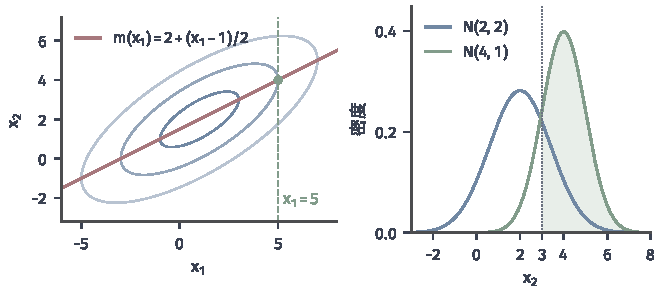
\includegraphics[width=112mm]{figures/01-basic-mathematics/05-probability-and-statistics-basics/matplotlib/rvec-gaussian-conditional/figure.pdf}
  \caption{二维高斯分布的条件化，参数为$\bm\mu=(1,2)^{\top}$、$\Sigma_{1,1}=4$、$\Sigma_{1,2}=2$、$\Sigma_{2,2}=2$。(a)蓝色椭圆是马氏距离为$1,2,3$的等密度线；红线是条件均值$m(x_1)=2+(x_1-1)/2$；绿色虚线标出观测$x_1=5$，圆点为该处的条件均值$4$。(b)蓝线是观测前$X_2$的边缘密度$\mathcal N(2,2)$，绿线是给定$X_1=5$后的条件密度$\mathcal N(4,1)$；阴影面积$\mathbb P(X_2>3\mid X_1=5)\approx0.84$。}
  \label{fig:rvec-gaussian-conditional}
\end{figure}

二维情形的公式可以用相关系数改写：$\mathbb E[X_2\mid X_1=x_1]=\mu_2+\rho\frac{\sigma_2}{\sigma_1}(x_1-\mu_1)$，$\operatorname{Var}(X_2\mid X_1=x_1)=\sigma_2^2(1-\rho^2)$。本例$\rho^2=1/2$，条件方差恰为边缘方差的一半；$|\rho|$越接近$1$，观测$X_1$后$X_2$的剩余不确定性越小。与示例~\ref{ex:rvec-study-table}中随$x$变化的条件方差相比，“条件方差不依赖观测值”是高斯模型的特殊性质。条件均值关于观测是一条直线，这也是第~\ref{sec:pred-regression}节简单线性回归模型的概率背景。

\FloatBarrier
\section{本章小结}
\label{sec:rvec-summary}

联合分布描述几个随机变量在同一次试验中的共同取值，可以用联合质量函数、联合密度或联合分布函数表示。边缘分布由联合分布求和或积分得到，但边缘相同的联合分布可以截然不同。均值向量描述共同的中心，协方差矩阵通过$\operatorname{Var}(\bm a^{\top}\bm X)=\bm a^{\top}\bm\Sigma\bm a$概括所有线性组合的波动；相关系数只度量线性关联，协方差矩阵奇异则对应以概率$1$成立的线性约束。

独立与条件分布从两个方向描述变量之间的信息。独立要求联合分布分解为边缘之积，它推出不相关，反之不成立；两两独立也推不出相互独立。条件分布由联合分布按观测值切片再归一化得到，全概率、全期望和全方差公式把条件层面的量汇总回总体。条件独立与无条件独立互不蕴含：共享的未知参数会让条件独立的观测在边缘上相关。

变换与生成是方向相反的两个问题。多元变量替换、卷积和辅助变量方法从已知分布计算组合量的分布，由此得到了二项分布、Gamma分布与Beta分布之间的联系；逆变换采样与按条件分解逐个生成，则从均匀输入出发构造目标分布，混合分布与层次模型都是条件生成的例子。

多元高斯分布把这些操作汇集在两个参数上：由独立标准高斯变量经$\bm\mu+\bm L\bm Z$生成，仿射变换后仍是高斯，边缘化只需取子向量与子矩阵，零交叉协方差即推出独立，条件分布的均值是观测的仿射函数、协方差是Schur补。本章始终假定分布已知；下一章转向相反的问题：只观察到数据时，怎样构造统计量并估计未知的分布参数（第~\ref{chap:sample-estimation}章）。

\chapter{样本、统计量与参数估计}
\label{chap:sample-estimation}

前两章总是先给定分布，再计算事件的概率、期望和方差。实际工作中的方向常常相反：一批产品的不合格率、一台仪器读数的平均水平都不知道，我们手里只有有限次检验或测量的结果，需要由这些结果反过来说出总体规律的某个数值。本章研究这一步怎样落实为明确的数学对象和计算方法。

为了便于比较，全章反复使用两组数据，它们都是为说明方法而设定的教学示例。第一组是从一条生产线上抽检的$10$件产品，以$1$表示不合格、$0$表示合格，结果为
\[
0,\ 0,\ 1,\ 0,\ 0,\ 0,\ 1,\ 0,\ 0,\ 0,
\]
共有$2$件不合格。第二组是对同一零件长度的$8$次测量读数（单位mm）：
\[
9.8,\ 10.1,\ 10.0,\ 10.3,\ 10.1,\ 9.9,\ 10.4,\ 10.2 .
\]
我们关心的问题是：不合格的概率大约是多少？零件长度的平均水平和测量的分散程度大约是多少？

回答这些问题需要四步。我们先说明“总体规律”和“一组数据”分别对应什么数学对象，并区分由数据算出的统计量、用于估计的估计量和代入数据后的估计值。接着不借助任何模型，用经验分布、样本矩、样本方差和样本分位数描述数据本身。然后分别利用三类信息构造估计：矩估计让模型的矩与样本矩相等，最大似然估计寻找最能产生当前数据的参数，基于后验的估计再把对参数的先验认识与数据合并。本章只说明估计怎样定义、怎样计算；同一参数的不同估计谁更准确、误差有多大，留给第~\ref{chap:sampling-errors}章回答。

\section{总体、样本与统计模型}
\label{sec:est-samples}

在构造任何估计之前，我们先要说清楚三件事：想了解的总体规律用什么表示，手中的数据与这个规律是什么关系，以及“从数据算出的数”在数学上是什么。

\subsection{总体与未知参数}

\paragraph{总体规律落实为分布}
对生产线，我们想知道的是“任取一件产品时它不合格的可能性”；对测量，我们想知道的是“再测一次时读数的分布情况”。这些都是关于一类试验的概率规律，而不是关于某一件产品或某一次读数的结论。我们把所研究的对象的全体称为\term{总体}（population），并把总体规律落实为一个概率分布：一件产品是否不合格对应一个取值于$\{0,1\}$的随机变量的分布，一次读数对应一个实值随机变量的分布。

总体分布通常并不完全未知。经验或问题结构往往告诉我们分布属于哪一类，只有其中少数几个数值不确定。例如，“合格或不合格”只有两个结果，其分布必然是Bernoulli分布，未知的只是不合格概率；读数受许多微小因素共同影响，常用高斯分布描述，未知的是均值与方差。这样，“了解总体”就化为“确定少数未知数值”。

\paragraph{统计模型与参数}
我们把这种“分布类型已知、少数数值未知”的设定写成一个分布族。

\begin{definition}[统计模型与参数]
\label{def:est-statistical-model}
设$\Theta$是一个集合，对每个$\theta\in\Theta$给定一个概率分布$F_\theta$。分布族$\{F_\theta:\theta\in\Theta\}$称为一个（参数）\term{统计模型}（statistical model），$\theta$称为参数，$\Theta$称为\term{参数集}（parameter set）。离散情形下记$F_\theta$的质量函数为$p(x;\theta)$，连续情形下记其密度为$f(x;\theta)$。
\end{definition}

模型假定总体分布等于族中的某一个$F_{\theta}$，但不知道是哪一个。参数集规定了参数的合理取值，例如概率必须在$[0,1]$中，方差必须为正。参数可以是一个数，也可以是一个向量，如高斯模型的$\theta=(\mu,\sigma^2)$。

\begin{example}[三个常用模型]
\label{ex:est-three-models}
下面三个模型对应本章的三类问题，它们的质量函数或密度见第~\ref{sec:prob-discrete-models}节和第~\ref{sec:prob-gaussian}节。
\begin{itemize}
  \item 不合格率：$X\sim\operatorname{Bernoulli}(p)$，$\mathbb{P}(X=x)=p^x(1-p)^{1-x}$，$x\in\{0,1\}$，参数集$\Theta=[0,1]$。
  \item 单位时间内的事件数，如一天中收到的投诉次数：$X\sim\operatorname{Poisson}(\lambda)$，$\mathbb{P}(X=x)=e^{-\lambda}\lambda^x/x!$，$x=0,1,2,\dots$，参数集$\Theta=(0,\infty)$。
  \item 测量读数：$X\sim\mathcal{N}(\mu,\sigma^2)$，参数$\theta=(\mu,\sigma^2)$，参数集$\Theta=\mathbb{R}\times(0,\infty)$。若仪器的测量标准差已经标定，$\sigma^2$已知，则只有$\mu$是参数，$\Theta=\mathbb{R}$。
\end{itemize}
同一个“读数”问题，因$\sigma^2$是否已知而对应两个不同的模型；参数是什么由模型设定决定，而不是由数据决定。
\end{example}

\paragraph{两种不确定性}
统计模型里同时有两种不确定性，需要分开看待。第一种是个体的随机波动：即使$p$已知为$0.2$，下一件产品是否不合格仍然不能预先确定，这由分布$F_\theta$描述。第二种是对参数的未知：$p$本身是一个确定的数，只是我们不知道它。前者不会因为多做试验而消失，后者则会随着数据增加而逐渐减少。在第~\ref{sec:est-bayes}节之前，本章都把参数看作未知的常数；到那一节再用概率分布表示第二种不确定性。

\subsection{随机样本与抽样方式}

\paragraph{抽样前与抽样后}
数据与总体的联系建立在“数据是从总体中抽取的”这一假设上。在检验之前，第$i$件产品是否不合格还不知道，它是一个随机变量$X_i$；检验之后我们得到一个具体的数$x_i$，它是$X_i$的一次实现。同一个符号在抽样前后含义不同：大写的$X_1,\dots,X_n$是随机变量，用来讨论“如果重复抽样，会得到什么样的数据”；小写的$x_1,\dots,x_n$是手中的数值，用来计算。

\begin{definition}[随机样本]
\label{def:est-random-sample}
若随机变量$X_1,\dots,X_n$相互独立，且每个$X_i$都服从总体分布$F$，则称它们为来自$F$的容量为$n$的\term{随机样本}（random sample），也称\term{独立同分布}（independent and identically distributed，i.i.d.）样本，记作$X_1,\dots,X_n\overset{\text{i.i.d.}}{\sim}F$。它们的一组实现$x_1,\dots,x_n$称为观测值或数据。
\end{definition}

定义中的两项条件约束的内容不同。“同分布”要求每次观测都来自同一总体，例如测量期间仪器没有漂移、产品来自同一条生产线；“独立”要求一次观测的结果不影响另一次观测的分布，例如前一件产品不合格并不改变下一件不合格的概率。

\paragraph{样本的联合分布}
独立性使样本的联合分布可以由单个分布直接写出。第~\ref{sec:rvec-independence}节说明，相互独立的随机变量的联合质量函数（或联合密度）等于各自质量函数（或密度）的乘积。因此，在统计模型$\{F_\theta\}$下，样本$X_1,\dots,X_n$的联合质量函数或联合密度为
\begin{equation}
\label{eq:est-sample-joint}
p(x_1,\dots,x_n;\theta)=\prod_{i=1}^n p(x_i;\theta),
\qquad
f(x_1,\dots,x_n;\theta)=\prod_{i=1}^n f(x_i;\theta).
\end{equation}
这个乘积形式是后面似然函数和后验分布计算的出发点。

\begin{example}[抽检数据的联合概率]
\label{ex:est-joint-bernoulli}
在Bernoulli模型下，抽检数据$(0,0,1,0,0,0,1,0,0,0)$出现的概率为
\[
\prod_{i=1}^{10}p^{x_i}(1-p)^{1-x_i}=p^{\sum_i x_i}(1-p)^{10-\sum_i x_i}=p^2(1-p)^8 .
\]
它只依赖于不合格件数$2$，与不合格品出现在第几次检验无关。例如$p=0.2$时，这个概率为$0.2^2\times0.8^8\approx0.00671$。
\end{example}

\paragraph{一组观测不必是独立同分布样本}
“独立同分布”是对抽样方式的假设，不是数据自带的性质。下面三种情形对照起来看最清楚。
\begin{itemize}
  \item 独立重复测量：同一仪器在稳定条件下反复测量同一零件，每次读数的误差互不影响，这是独立同分布假设最自然的场景。
  \item 有限总体的不放回抽样：从一个有限的批次中逐件取出检验、不再放回，每次抽取会改变剩余产品的构成，于是各次结果不独立。
  \item 时间序列：按时间记录的数据，如每日气温或逐小时销量，相邻观测往往相互关联，还可能随季节改变分布，独立和同分布两项都可能不成立。
\end{itemize}

\begin{example}[不放回抽样破坏独立性]
\label{ex:est-without-replacement}
一批$10$件产品中恰有$2$件不合格。随机取出一件检验后不放回，再取一件。记$X_1,X_2$分别表示两次取到的产品是否不合格。由对称性，第二次单独来看仍有$\mathbb{P}(X_2=1)=2/10$，所以$X_1,X_2$同分布；但
\[
\mathbb{P}(X_2=1\mid X_1=1)=\frac{1}{9}\neq\frac{2}{10}=\mathbb{P}(X_2=1),
\]
第一件的结果改变了第二件的条件概率，两者不独立。若批次很大而抽取的件数很少，这种影响很小，可以近似当作独立同分布样本处理；本章例子中的生产线抽检正是按这种近似处理的。
\end{example}

\subsection{统计量、估计量与估计值}

\paragraph{统计量}
有了样本，我们要从中算出一些数。最直接的是样本平均$\frac1n\sum_{i}X_i$，它把$n$个观测压缩为一个数；对测量数据，也可能关心最大读数$\max_iX_i$。这些量的共同点是：给定数据就能直接算出，计算规则中不出现任何未知参数。

\begin{definition}[统计量]
\label{def:est-statistic}
设$X_1,\dots,X_n$是样本，$T$是一个确定的函数，其表达式不依赖未知参数。称$T(X_1,\dots,X_n)$为一个\term{统计量}（statistic）。
\end{definition}

统计量是样本的函数，所以它在抽样前是随机变量，有自己的分布；抽样后把数据代入，得到一个数。像$\bar X-\mu$这样的量，当$\mu$未知时就不是统计量，因为拿到数据后也算不出它的值。样本均值、样本方差和顺序统计量都是统计量，第~\ref{sec:est-sample-features}节将逐一介绍。

\paragraph{估计量与估计值}
当一个统计量被用来猜测某个参数或参数的函数$g(\theta)$时，我们换一个名称，强调它的用途。

\begin{definition}[估计量与估计值]
\label{def:est-estimator}
用于估计$g(\theta)$的统计量$T(X_1,\dots,X_n)$称为$g(\theta)$的\term{估计量}（estimator），常记作$\hat\theta_n$；将观测值代入后得到的数$T(x_1,\dots,x_n)$称为\term{估计值}（estimate）。
\end{definition}

估计量是一个规则，也是一个随机变量；估计值是这个规则用于一组具体数据的结果；参数$\theta$则是一个确定但未知的数。三者的关系如图~\ref{fig:est-population-sample-estimate}所示：上行是抽样之前的随机对象，下行是抽样之后的数值，同一个计算规则$T$既作用于随机样本，也作用于观测数据。第~\ref{chap:sampling-errors}章研究估计量的分布，正是为了回答“若重复抽样，这条规则给出的估计值会怎样波动”。

\begin{figure}[htbp]
  \centering
  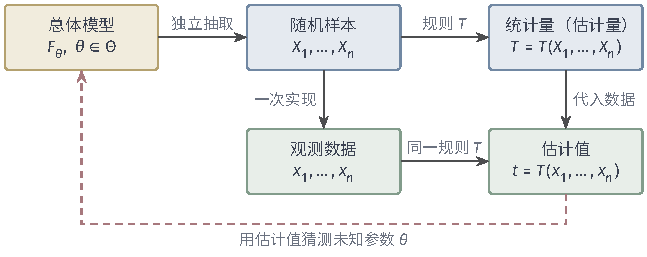
\includegraphics[width=109.6mm]{figures/01-basic-mathematics/05-probability-and-statistics-basics/tikz/est-population-sample-estimate/figure.pdf}
  \caption{总体模型、样本、统计量与估计值的关系。上行（蓝框）是抽样前的随机对象：从总体$F_\theta$独立抽取得到随机样本，再按规则$T$得到统计量（用于估计时称估计量）。下行（绿框）是一次抽样后的数值：观测数据代入同一规则得到估计值。红色虚线表示用估计值去猜测未知参数$\theta$，它是推断而不是计算。}
  \label{fig:est-population-sample-estimate}
\end{figure}

\begin{example}[同一参数的两个估计量]
\label{ex:est-two-estimators}
对测量读数的平均水平$\mu$，样本均值$\frac18\sum_{i=1}^8X_i$是一个估计量，代入读数得估计值$10.1$。“最大读数与最小读数的中点”$\frac12(\max_iX_i+\min_iX_i)$也是一个估计量，代入后得$\frac12(10.4+9.8)=10.1$。两条规则对这组数据恰好给出相同的估计值，但它们是不同的估计量：换一组数据，结果一般就不同了。比较哪条规则更可靠，需要看它们在重复抽样下的表现，这是第~\ref{chap:sampling-errors}章的任务。
\end{example}

\section{经验分布与样本的数值特征}
\label{sec:est-sample-features}

在给出任何模型之前，我们先描述数据本身。第~\ref{chap:random-variables}章用分布函数、期望、方差和分位数描述一个分布；本节把同样的工具用于“把每个观测看成等可能出现”的分布，得到经验分布函数、样本矩、样本方差和样本分位数。

\subsection{经验分布函数}
\label{sec:est-empirical-cdf}

\paragraph{定义与读法}
总体分布函数$F(t)=\mathbb{P}(X\le t)$给出随机变量不超过阈值$t$的概率。手中只有数据时，最自然的替代是数一数有多少个观测不超过$t$，再除以样本量。

\begin{definition}[经验分布函数]
\label{def:est-empirical-cdf}
设$X_1,\dots,X_n$是样本。函数
\begin{equation}
\label{eq:est-empirical-cdf}
\hat F_n(t)=\frac1n\sum_{i=1}^n\mathbb{I}\{X_i\le t\},\qquad t\in\mathbb{R}
\end{equation}
称为\term{经验分布函数}（empirical distribution function），其中$\mathbb{I}\{X_i\le t\}$在$X_i\le t$时取$1$，否则取$0$。在每个观测值上放置概率$1/n$所得的离散分布称为\term{经验分布}（empirical distribution），$\hat F_n$正是它的分布函数。
\end{definition}

$\hat F_n$是一个阶梯函数：它在最小观测值左侧为$0$，在最大观测值处及其右侧为$1$，只在观测值处向上跳跃。若某个值$v$在样本中出现$m$次，则$\hat F_n$在$v$处跳$m/n$；在相邻两个不同观测值之间保持不变。与任何分布函数一样，它右连续，即跳跃点处取跳跃后的值。

\begin{example}[含重复值的读数]
\label{ex:est-ecdf-readings}
将$8$次读数排序为$9.8$、$9.9$、$10.0$、$10.1$、$10.1$、$10.2$、$10.3$、$10.4$，其中$10.1$出现两次。于是
\[
\hat F_8(t)=
\begin{cases}
0, & t<9.8,\\
1/8, & 9.8\le t<9.9,\\
2/8, & 9.9\le t<10.0,\\
3/8, & 10.0\le t<10.1,\\
5/8, & 10.1\le t<10.2,\\
6/8, & 10.2\le t<10.3,\\
7/8, & 10.3\le t<10.4,\\
1, & t\ge10.4 .
\end{cases}
\]
在$10.1$处函数从$3/8$跳到$5/8$，跳跃大小$2/8$等于该值出现的次数除以$8$。例如$\hat F_8(10.15)=5/8$，表示有$62.5\%$的读数不超过$10.15$。
\end{example}

\paragraph{与总体分布函数的区别}
图~\ref{fig:est-empirical-cdf}把这个阶梯与一条假想的总体分布函数画在一起。两者描述的对象不同：总体分布函数$F$是一个确定的函数，描述总体规律；经验分布函数$\hat F_n$只描述当前这$8$个数的累计频率。抽样前，对每个固定的$t$，$\hat F_n(t)$是$n$个取值于$\{0,1\}$的独立随机变量的平均，因此本身是随机变量；换一组数据，阶梯的位置和高度都会改变。图中阶梯大体贴近光滑曲线，但在多处偏离。样本量增大时$\hat F_n(t)$是否会趋于$F(t)$、偏离有多大，属于抽样误差问题，将在第~\ref{sec:samp-lln}节讨论。

\begin{figure}[htbp]
  \centering
  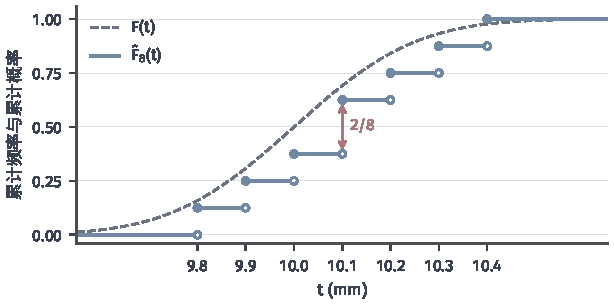
\includegraphics[width=104mm]{figures/01-basic-mathematics/05-probability-and-statistics-basics/matplotlib/est-empirical-cdf/figure.pdf}
  \caption{$8$次读数的经验分布函数（蓝色阶梯）与一条假想的总体分布函数（灰色虚线，取$\mathcal{N}(10.0,0.2^2)$仅作对照）。实心点表示跳跃点处的函数值，空心点表示跳跃前的极限；读数$10.1$出现两次，所以该处跳跃高度为$2/8$，其余各处为$1/8$。}
  \label{fig:est-empirical-cdf}
\end{figure}

\subsection{样本均值与样本矩}

\paragraph{样本均值}
经验分布把概率$1/n$放在每个观测上，按第~\ref{sec:prob-expectation}节的定义，它的期望就是
\begin{equation}
\label{eq:est-sample-mean}
\bar X_n=\frac1n\sum_{i=1}^nX_i ,
\end{equation}
称为\term{样本均值}（sample mean）。不致混淆时省略下标，记作$\bar X$。若数据中有重复值，也可以按不同取值分组：设不同取值为$v_1,\dots,v_m$，各出现$c_1,\dots,c_m$次，则$\bar x=\sum_{j=1}^m v_j\cdot\frac{c_j}{n}$，即“取值乘以频率再求和”，这与离散分布期望的公式完全一致。对读数数据，
\[
\bar x=\frac{9.8+10.1+10.0+10.3+10.1+9.9+10.4+10.2}{8}=\frac{80.8}{8}=10.1 ;
\]
对抽检数据，$\bar x=2/10=0.2$，即不合格品所占比例。

\paragraph{样本原点矩与中心矩}
样本均值只给出数据的位置。第~\ref{chap:random-variables}章用$\mathbb{E}X^k$提取分布的其他数值信息，样本上同样可以对观测的幂取平均。

\begin{definition}[样本矩]
\label{def:est-sample-moments}
设$X_1,\dots,X_n$是样本，$k$为正整数。称
\[
m_k=\frac1n\sum_{i=1}^nX_i^k
\qquad\text{与}\qquad
\hat\mu_k=\frac1n\sum_{i=1}^n(X_i-\bar X)^k
\]
分别为$k$阶\term{样本原点矩}（sample raw moment）和$k$阶\term{样本中心矩}（sample central moment），统称\term{样本矩}（sample moment）。
\end{definition}

原点矩以$0$为参照，中心矩以样本均值为参照。一阶原点矩就是样本均值；一阶中心矩恒为$0$，因为$\sum_i(X_i-\bar X)=0$；二阶中心矩度量观测围绕均值的分散程度。两者可以互相换算，例如展开平方得
\begin{equation}
\label{eq:est-second-moment-identity}
\hat\mu_2=\frac1n\sum_{i=1}^n(X_i^2-2\bar XX_i+\bar X^2)=m_2-2\bar X\cdot\bar X+\bar X^2=m_2-\bar X^2 .
\end{equation}

\begin{example}[读数的样本矩]
\label{ex:est-reading-moments}
读数与均值$10.1$的离差为$-0.3$、$0$、$-0.1$、$0.2$、$0$、$-0.2$、$0.3$、$0.1$，平方和为$0.28$，所以$\hat\mu_2=0.28/8=0.035$。另一方面，$m_2=\frac18\sum_ix_i^2=102.045$，按式~\eqref{eq:est-second-moment-identity}有$m_2-\bar x^2=102.045-102.01=0.035$，两种算法一致。离差关于$0$正负对称，所以三阶中心矩$\hat\mu_3=0$；四阶中心矩$\hat\mu_4=(2\times0.3^4+2\times0.2^4+2\times0.1^4)/8=0.00245$。
\end{example}

\paragraph{能算出不等于总体矩存在}
任意有限个实数都能算出任意阶样本矩，但这并不说明对应的总体矩存在。例如标准Cauchy分布的密度为$f(x)=\frac{1}{\pi(1+x^2)}$，由于$\int_0^\infty\frac{x}{\pi(1+x^2)}\,\mathrm{d}x=\lim_{b\to\infty}\frac{\ln(1+b^2)}{2\pi}=\infty$，它的期望不存在。从这个分布抽出的样本仍然有样本均值，只是这个数并不对应任何总体均值。用样本矩去推断总体矩之前，必须先确认后者存在。

\subsection{样本方差}
\label{sec:est-sample-variance}

\paragraph{两种分母}
描述数据的分散程度，最直接的是平方离差的平均$\hat\sigma_n^2=\frac1n\sum_i(X_i-\bar X)^2$，也就是二阶样本中心矩$\hat\mu_2$。实际中更常用的是把分母换成$n-1$的版本。

\begin{definition}[样本方差]
\label{def:est-sample-variance}
设$n\ge2$。称
\begin{equation}
\label{eq:est-sample-variance}
S_n^2=\frac{1}{n-1}\sum_{i=1}^n(X_i-\bar X_n)^2
\end{equation}
为\term{修正样本方差}（corrected sample variance），通常简称\term{样本方差}（sample variance）；称$S_n=\sqrt{S_n^2}$为\term{样本标准差}（sample standard deviation）。分母为$n$的$\hat\sigma_n^2=\frac{n-1}{n}S_n^2$称为未修正的样本方差。
\end{definition}

对读数数据，平方离差和为$0.28$，所以$\hat\sigma^2=0.28/8=0.035$，$S^2=0.28/7=0.04$，$S=0.2$。两者相差一个因子$8/7$。样本量越大，这个因子越接近$1$；样本量很小时，差别不能忽略。为什么要除以$n-1$，可以从期望的计算中看出来。

\paragraph{期望的计算}
下面的定理在独立同分布、总体方差有限的条件下计算平方离差和的期望。证明需要两个事实：期望是线性的；相互独立的随机变量之和的方差等于各方差之和（第~\ref{sec:rvec-moments}节），从而$\operatorname{Var}(\bar X_n)=\frac{1}{n^2}\sum_i\operatorname{Var}(X_i)=\sigma^2/n$。

\begin{theorem}[平方离差和的期望]
\label{thm:est-sample-variance-expectation}
设$n\ge2$，$X_1,\dots,X_n$独立同分布，$\mathbb{E}X_1=\mu$，$\operatorname{Var}(X_1)=\sigma^2<\infty$。则
\[
\mathbb{E}\Big[\sum_{i=1}^n(X_i-\bar X_n)^2\Big]=(n-1)\sigma^2,
\qquad\text{从而}\qquad
\mathbb{E}S_n^2=\sigma^2,\quad \mathbb{E}\hat\sigma_n^2=\frac{n-1}{n}\sigma^2 .
\]
\end{theorem}

\begin{proof}
先把围绕真实均值$\mu$的平方和分解为两部分。将$X_i-\mu$写成$(X_i-\bar X_n)+(\bar X_n-\mu)$，展开平方并求和：
\[
\sum_{i=1}^n(X_i-\mu)^2=\sum_{i=1}^n(X_i-\bar X_n)^2+2(\bar X_n-\mu)\sum_{i=1}^n(X_i-\bar X_n)+n(\bar X_n-\mu)^2 .
\]
中间一项含因子$\sum_i(X_i-\bar X_n)=0$，因此
\begin{equation}
\label{eq:est-sum-of-squares-decomposition}
\sum_{i=1}^n(X_i-\bar X_n)^2=\sum_{i=1}^n(X_i-\mu)^2-n(\bar X_n-\mu)^2 .
\end{equation}
对右边逐项取期望。每个$X_i$的方差为$\sigma^2$，所以$\mathbb{E}\sum_i(X_i-\mu)^2=n\sigma^2$。又因$\mathbb{E}\bar X_n=\mu$，有$\mathbb{E}(\bar X_n-\mu)^2=\operatorname{Var}(\bar X_n)=\sigma^2/n$，故$\mathbb{E}\,n(\bar X_n-\mu)^2=\sigma^2$。两者相减得$(n-1)\sigma^2$。分别除以$n-1$和$n$即得后两个等式。
\end{proof}

式~\eqref{eq:est-sum-of-squares-decomposition}说明了修正因子的来源。围绕真实均值$\mu$的平方和平均为$n\sigma^2$，但$\mu$未知，我们只能围绕$\bar X_n$计算。$\bar X_n$是由同一组数据算出的，它总是落在数据“中间”，使平方和比围绕$\mu$时更小，平均少了一个$\sigma^2$。除以$n-1$恰好补偿了这部分损失。注意定理需要$n\ge2$：只有一个观测时，离差恒为$0$，无法从数据中看出分散程度。

一个估计量的期望是否等于被估计的量，只是评价估计的一个角度；除以$n-1$的估计并不在所有意义下都更好。估计的系统误差、波动和均方误差怎样定义和比较，留到第~\ref{sec:samp-errors}节统一讨论。

\begin{example}[两个观测的平方离差]
\label{ex:est-two-observations}
取$n=2$。此时$\bar X=\frac{X_1+X_2}2$，$\sum_i(X_i-\bar X)^2=\frac{(X_1-X_2)^2}{2}$。由于$X_1-X_2$的均值为$0$，方差为$2\sigma^2$，有$\mathbb{E}(X_1-X_2)^2=2\sigma^2$，所以平方离差和的期望为$\sigma^2=(2-1)\sigma^2$，与定理一致。若误用分母$n=2$，得到的$\hat\sigma^2$平均只有$\sigma^2/2$。
\end{example}

\subsection{样本分位数}

\paragraph{顺序统计量}
分位数描述分布的位置而不是平均，它需要把数据排序。

\begin{definition}[顺序统计量]
\label{def:est-order-statistics}
把样本$X_1,\dots,X_n$从小到大排列为$X_{(1)}\le X_{(2)}\le\dots\le X_{(n)}$，称$X_{(k)}$为第$k$个\term{顺序统计量}（order statistic）。
\end{definition}

$X_{(1)}=\min_iX_i$与$X_{(n)}=\max_iX_i$分别是样本最小值和最大值，二者之差$X_{(n)}-X_{(1)}$称为极差。位于中间位置的顺序统计量给出数据的“中心”：它左右两侧的观测个数大致相等，与样本均值不同，它不受个别极端值的大小影响。对读数数据，$x_{(1)}=9.8$，$x_{(8)}=10.4$，$x_{(4)}=x_{(5)}=10.1$。

\paragraph{由经验分布函数定义分位数}
第~\ref{sec:prob-numerical-features}节用分布函数的广义逆定义总体分位数：$p$分位数是使$F(t)\ge p$的最小$t$。对经验分布函数做同样的操作，就得到样本分位数。

\begin{definition}[样本分位数]
\label{def:est-sample-quantile}
设$0<p<1$。称
\begin{equation}
\label{eq:est-sample-quantile}
\hat q_p=\min\{t\in\mathbb{R}:\hat F_n(t)\ge p\}=X_{(\lceil np\rceil)}
\end{equation}
为$p$\term{样本分位数}（sample quantile），其中$\lceil np\rceil$是不小于$np$的最小整数。$p=1/2$时的样本分位数称为\term{样本中位数}（sample median）。
\end{definition}

第二个等号可以这样验证。$\hat F_n$在$X_{(k)}$处的值至少是$k/n$，而在$X_{(k)}$左侧的值至多是$(k-1)/n$。因此使$\hat F_n(t)\ge p$的最小$t$，就是满足$k/n\ge p$的最小$k$所对应的$X_{(k)}$，即$k=\lceil np\rceil$。

\paragraph{不同的约定}
当$np$恰为整数时，$\hat F_n$在$X_{(np)}$与$X_{(np+1)}$之间恰好等于$p$，整段区间上的点都“处于$p$的位置”，取左端点只是一种选择。常见的约定有以下几种。
\begin{itemize}
  \item 广义逆：按式~\eqref{eq:est-sample-quantile}取$X_{(\lceil np\rceil)}$。
  \item 跳跃处取中点：$np$为整数时取$\frac12(X_{(np)}+X_{(np+1)})$，否则同上。偶数样本的中位数$\frac12(X_{(n/2)}+X_{(n/2+1)})$就是这种约定在$p=1/2$时的结果。
  \item 线性插值：令$h=(n-1)p+1$，取$X_{(\lfloor h\rfloor)}+(h-\lfloor h\rfloor)\big(X_{(\lfloor h\rfloor+1)}-X_{(\lfloor h\rfloor)}\big)$，即把第$k$个顺序统计量放在$p=(k-1)/(n-1)$处，相邻两点之间用直线连接。
\end{itemize}
图~\ref{fig:est-sample-quantiles}把广义逆与线性插值两种约定看成$p$的函数画了出来：广义逆是经验分布函数阶梯的“反函数”，也呈阶梯形，在$p$越过每个$k/n$时跳到下一个顺序统计量；线性插值则是一条穿过各顺序统计量的折线。

\begin{example}[读数的四分位数与中位数]
\label{ex:est-quantile-conventions}
对$8$个读数取$p=0.25$，$np=2$是整数。广义逆给出$x_{(2)}=9.9$；跳跃处取中点给出$\frac12(9.9+10.0)=9.95$；线性插值中$h=7\times0.25+1=2.75$，给出$9.9+0.75\times(10.0-9.9)=9.975$。三种约定得到三个不同的值。

对中位数，三种约定都给出$10.1$，因为两个中间值$x_{(4)}=x_{(5)}=10.1$相同。若只取前$6$个读数，排序后为$9.8,9.9,10.0,10.1,10.1,10.3$，中间两个值是$10.0$与$10.1$：广义逆给出$x_{(3)}=10.0$，后两种约定都给出$10.05$。
\end{example}

\begin{figure}[htbp]
  \centering
  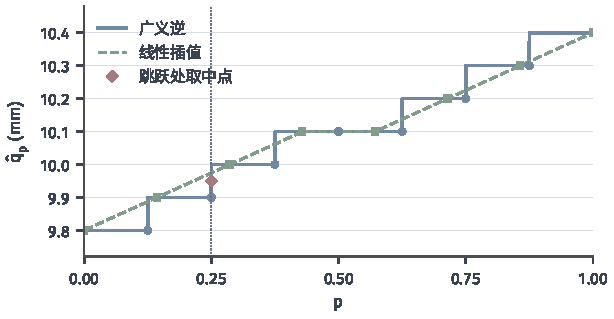
\includegraphics[width=104mm]{figures/01-basic-mathematics/05-probability-and-statistics-basics/matplotlib/est-sample-quantiles/figure.pdf}
  \caption{$8$个读数的样本分位数$\hat q_p$随$p$的变化。蓝色阶梯是经验分布函数的广义逆，圆点标出它在$p=k/8$处取到的顺序统计量$x_{(k)}$；绿色虚线是线性插值约定，方点位于$p=(k-1)/7$。在$p=0.25$（点线）处，广义逆取$9.9$，跳跃处取中点得$9.95$（菱形），线性插值得$9.975$。}
  \label{fig:est-sample-quantiles}
\end{figure}

不同统计软件默认采用的约定并不相同，样本量较小时，同一组数据可能报告出不同的分位数。这些差别局限在$p$所在位置附近的少数几个顺序统计量之间，样本量增大、数据变密时一般会缩小。报告分位数时，应当说明所用的约定。

\section{矩估计}
\label{sec:est-moments}

上一节的样本矩只描述数据。如果再给出统计模型，总体矩就成了参数的函数；让总体矩等于样本矩，便得到关于参数的方程。这是构造估计最直接的方法。

\subsection{矩估计的构造}

\paragraph{估计方程}
在统计模型$\{F_\theta:\theta\in\Theta\}$下，设$X\sim F_\theta$的$k$阶矩存在，把它记作
\[
\mu_k(\theta)=\mathbb{E}_\theta X^k ,
\]
下标$\theta$提示期望是在分布$F_\theta$下计算的。$\mu_k(\theta)$是参数的一个已知函数，而样本原点矩$m_k$可以由数据算出。若参数有$d$个分量，我们选取$d$个矩，令它们分别等于对应的样本矩：
\begin{equation}
\label{eq:est-moment-equations}
\mu_k(\theta)=m_k,\qquad k=1,\dots,d .
\end{equation}

\begin{definition}[矩估计]
\label{def:est-method-of-moments}
若方程组~\eqref{eq:est-moment-equations}在$\Theta$中有唯一解，则称这个解$\hat\theta_n$为$\theta$的\term{矩估计}（method of moments estimator）。
\end{definition}

这一做法的依据是第~\ref{sec:est-sample-features}节的观察：样本矩是经验分布的矩，而经验分布描述了数据的累计频率。若经验分布接近总体分布，它们的矩也应当接近，于是解出的参数应当接近真实参数。这种“接近”在什么条件下成立，第~\ref{sec:samp-consistency}节再作说明。

\paragraph{计算步骤}
矩估计的计算可以按四步组织：
\begin{enumerate}
  \item 选择矩：确定使用哪几阶矩，也可以使用中心矩或其他函数的期望；
  \item 建立方程：把所选总体矩写成参数的函数，令其等于对应样本矩；
  \item 求解参数：解方程组，得到用样本矩表示的参数；
  \item 检查范围：确认解存在、唯一，并落在参数集$\Theta$中。
\end{enumerate}
第一步中，方程个数等于参数个数只是一个计数条件，并不保证方程组相互独立或可解。例如对只取$0$和$1$的随机变量，总有$X^k=X$，所以各阶原点矩全部等于$\mathbb{E}X$：无论选择几阶原点矩，得到的都是同一个方程。若模型有两个参数，而数据只取$0$和$1$，原点矩就不足以确定参数。第四步的检查同样不能省略，本节最后一小节将给出解不存在、不唯一或与数据矛盾的例子。

\subsection{矩估计的计算}

\paragraph{单参数模型}
单参数模型只需一个方程，通常选一阶矩。

\begin{example}[Bernoulli与Poisson模型]
\label{ex:est-mom-bernoulli-poisson}
在Bernoulli模型下，$\mu_1(p)=\mathbb{E}_pX=p$，方程$p=m_1$直接给出$\hat p=\bar X$。对抽检数据，$\hat p=2/10=0.2$，即不合格率的矩估计就是样本中不合格品的比例。这个解总在$[0,1]$中，第四步自动满足。

在Poisson模型下，$\mathbb{E}_\lambda X=\lambda$，所以同样有$\hat\lambda=\bar X$。若某客服中心连续$8$天收到的投诉次数为$2,0,3,1,2,4,1,3$（教学示例），则$\hat\lambda=16/8=2$，即估计每天平均收到$2$次投诉。若$8$天都没有投诉，$\hat\lambda=0$不在参数集$(0,\infty)$中，此时矩估计不存在；这种边界情况在第~\ref{sec:est-mle}节还会遇到。
\end{example}

两个模型中样本均值都成为参数的估计，原因是参数恰好等于总体均值。若参数与均值的关系不是恒等的，就需要解方程。例如指数分布$f(x;\lambda)=\lambda e^{-\lambda x}$的均值为$1/\lambda$，方程$1/\lambda=\bar X$给出$\hat\lambda=1/\bar X$。

\paragraph{两参数高斯模型}
均值和方差都未知时，需要两个方程。高斯分布$\mathcal{N}(\mu,\sigma^2)$的前两阶原点矩为$\mu_1=\mu$，$\mu_2=\mathbb{E}X^2=\operatorname{Var}(X)+(\mathbb{E}X)^2=\sigma^2+\mu^2$。令它们等于样本矩：
\[
\mu=m_1,\qquad \sigma^2+\mu^2=m_2 .
\]
第一式给出$\hat\mu=\bar X$，代入第二式并利用式~\eqref{eq:est-second-moment-identity}，得
\begin{equation}
\label{eq:est-mom-gaussian}
\hat\mu=\bar X,\qquad \hat\sigma^2=m_2-\bar X^2=\frac1n\sum_{i=1}^n(X_i-\bar X)^2 .
\end{equation}
方差的矩估计正是分母为$n$的未修正样本方差。

\begin{example}[读数的矩估计]
\label{ex:est-mom-readings}
由例~\ref{ex:est-reading-moments}，$m_1=10.1$，$m_2=102.045$。按式~\eqref{eq:est-mom-gaussian}，$\hat\mu=10.1$，$\hat\sigma^2=102.045-10.1^2=0.035$，$\hat\sigma\approx0.187$。修正样本方差为$S^2=0.04$，比矩估计大$8/7$倍。
\end{example}

这里的分母为$n$不是计算失误，而是矩估计的直接结果：矩估计让模型方差等于经验分布的方差，而经验分布的方差的分母就是$n$。定理~\ref{thm:est-sample-variance-expectation}表明，这个估计的期望是$\frac{n-1}{n}\sigma^2$，略小于$\sigma^2$。两种分母各自的含义已经清楚，但哪一个“更好”需要先确定评价标准，留给第~\ref{sec:samp-errors}节。

\subsection{解的存在性与适用条件}

\paragraph{需要检查的三件事}
矩估计的方程容易写出，但不能直接认为它给出了合理的估计。使用前至少要检查三点：所选的总体矩是否存在，否则方程本身没有意义（如前述Cauchy分布）；所选的矩能否确定待估参数，即不同参数是否对应不同的矩；解是否存在、唯一，并且与参数集及数据相容。下面两个例子分别对应后两点。

\begin{example}[解与数据矛盾]
\label{ex:est-mom-uniform}
设$X\sim\operatorname{U}(0,\theta)$，$\theta>0$未知。由$\mathbb{E}_\theta X=\theta/2$得矩估计$\hat\theta=2\bar X$。若观测为$0.2,\ 0.3,\ 1.9$，则$\bar x=0.8$，$\hat\theta=1.6$。但数据中已经有观测$1.9>1.6$，而在$\operatorname{U}(0,1.6)$下不可能出现大于$1.6$的值。这个估计值虽然在参数集$(0,\infty)$中，却与数据本身矛盾。矩方程只用到数据的平均，没有用到“所有观测都不超过$\theta$”这一信息。
\end{example}

\begin{example}[只用二阶矩丢失符号]
\label{ex:est-mom-sign}
设$X\sim\mathcal{N}(\mu,1)$。若只用二阶矩，方程为$\mu^2+1=m_2$。对观测$-1.2,\ -0.8,\ -1.5,\ -0.5$，$m_2=(1.44+0.64+2.25+0.25)/4=1.145$，解得$\mu=\pm\sqrt{0.145}\approx\pm0.381$，两个解无法区分；而样本均值为$-1.0$，明确指向负值。原因在于$\mathbb{E}X^2$只取决于$\mu^2$，参数$\mu$与$-\mu$给出相同的二阶矩，二阶矩不能确定$\mu$的符号。更糟的是，若观测为$0.3,\ -0.2,\ 0.5$，$m_2\approx0.127<1$，方程无实数解。改用一阶矩$\mu=m_1$，两个问题都不出现。
\end{example}

\paragraph{高阶矩对极端观测敏感}
需要多个方程时，自然会想到使用三阶、四阶矩，但高阶矩有一个实际缺陷：它们对个别极端观测非常敏感。离差先取高次幂再平均，一个大的离差会被放大到压倒其他所有项。

\begin{example}[一个读数的错误]
\label{ex:est-moment-sensitivity}
若把读数中的$10.4$误记为$11.4$，样本均值从$10.1$变为$10.225$，只改变约$1\%$；二阶中心矩从$0.035$变为约$0.219$，增大到约$6$倍；四阶中心矩从$0.00245$变为约$0.244$，增大到约$100$倍。基于高阶矩的估计因此可能被一个异常值左右。
\end{example}

因此，矩估计适合于参数可以由低阶矩直接确定的模型。它计算简单，常用来得到初步估计，或者为后面需要迭代求解的方法提供初值。

\section{最大似然估计}
\label{sec:est-mle}

矩估计只使用数据的几个平均量。例~\ref{ex:est-mom-uniform}显示，这可能丢掉数据中的其他信息。另一种思路是直接利用模型给出的整个联合分布：在所有候选参数中，选择使当前数据出现的概率（或密度）最大的那一个。

\subsection{似然函数}

\paragraph{固定数据，变动参数}
式~\eqref{eq:est-sample-joint}给出的联合质量函数$p(x_1,\dots,x_n;\theta)$有两个自变量：数据和参数。计算概率时，我们固定$\theta$，看不同数据出现的可能性。估计时情形反过来：数据已经观察到，是固定的；未知的是$\theta$。于是我们把同一个表达式看作$\theta$的函数，比较不同参数下“观察到这组数据”的可能性大小。

\begin{definition}[似然函数]
\label{def:est-likelihood}
给定观测值$x_1,\dots,x_n$，称
\[
L(\theta)=L(\theta;x_1,\dots,x_n)=p(x_1,\dots,x_n;\theta)\quad\text{（离散情形）}
\]
或$L(\theta)=f(x_1,\dots,x_n;\theta)$（连续情形）为参数$\theta$的\term{似然函数}（likelihood function），$\theta\in\Theta$。若$L(\theta)>0$，称$\ell(\theta)=\ln L(\theta)$为\term{对数似然函数}（log-likelihood function）。
\end{definition}

对随机样本，由式~\eqref{eq:est-sample-joint}，似然是各观测概率或密度的乘积，对数似然是相应的和：
\begin{equation}
\label{eq:est-log-likelihood}
L(\theta)=\prod_{i=1}^n f(x_i;\theta),\qquad
\ell(\theta)=\sum_{i=1}^n\ln f(x_i;\theta) .
\end{equation}
因为对数函数严格递增，$L$与$\ell$在同样的参数处取最大值；而和比积更容易求导，所以计算时几乎总是使用对数似然。数值上，许多小于$1$的数连乘会迅速接近$0$，取对数也避免了这个问题。

\paragraph{似然不是参数的分布}
似然函数比较的是同一组数据在不同参数下的概率，它本身不是参数的概率分布。$L(\theta_1)>L(\theta_2)$表示“若参数为$\theta_1$，看到这组数据的可能性更大”，而不是“$\theta_1$为真的概率更大”。

\begin{example}[似然的积分不为一]
\label{ex:est-likelihood-not-density}
例~\ref{ex:est-joint-bernoulli}给出抽检数据的似然$L(p)=p^2(1-p)^8$，$p\in[0,1]$。把它看作$p$的函数在$[0,1]$上积分，利用Beta函数（第~\ref{sec:prob-beta}节）$\int_0^1p^{a-1}(1-p)^{b-1}\mathrm{d}p=\frac{(a-1)!\,(b-1)!}{(a+b-1)!}$（$a,b$为正整数），得
\[
\int_0^1p^2(1-p)^8\,\mathrm{d}p=\frac{2!\,8!}{11!}=\frac{1}{495}\neq1 .
\]
所以$L(p)$不是$p$的密度。似然只有比值有意义：把$L$乘以任何不依赖$\theta$的正常数，最大值的位置不变。
\end{example}

\subsection{最大似然估计的计算}

似然函数给出了比较参数的依据，自然的做法是在参数集中选出似然最大的参数。

\begin{definition}[最大似然估计]
\label{def:est-mle}
若存在$\hat\theta\in\Theta$，使得对所有$\theta\in\Theta$都有$L(\hat\theta)\ge L(\theta)$，则称$\hat\theta$为$\theta$的\term{最大似然估计}（maximum likelihood estimate，MLE）。把$\hat\theta$看作数据的函数时，得到最大似然估计量。
\end{definition}

计算通常分三步：写出对数似然；在参数集内部令导数为零，求出候选解；检查候选解确实是最大值点，并与边界及趋于无穷时的情形作比较。第三步不能省略，本节最后一小节会说明原因。

\paragraph{Bernoulli模型}
先看抽检数据。Bernoulli模型只有一个参数，对数似然是一元函数，可以直接用一元微分求最大值。

\begin{example}[不合格率的最大似然估计]
\label{ex:est-mle-bernoulli}
设$X_1,\dots,X_n\overset{\text{i.i.d.}}{\sim}\operatorname{Bernoulli}(p)$，记不合格件数$k=\sum_ix_i$。似然为$L(p)=p^k(1-p)^{n-k}$。设$0<k<n$，对$p\in(0,1)$，
\[
\ell(p)=k\ln p+(n-k)\ln(1-p),\qquad
\ell'(p)=\frac{k}{p}-\frac{n-k}{1-p}.
\]
令$\ell'(p)=0$，得$k(1-p)=(n-k)p$，即$p=k/n$。又$\ell''(p)=-\frac{k}{p^2}-\frac{n-k}{(1-p)^2}<0$，$\ell$在$(0,1)$上严格凹（第~\ref{chap:univariate-differentiation}章），所以$k/n$是$(0,1)$上唯一的最大值点；而在两个端点处$L(0)=L(1)=0$，比内部的值都小。因此$\hat p=k/n=\bar x$。对抽检数据，$\hat p=2/10=0.2$，与矩估计相同。
\end{example}

图~\ref{fig:est-bernoulli-loglik}的左图画出了$n=10$、$k=2$时的对数似然：曲线在$p=0.2$处取最大值，向两侧下降，靠近$p=0$和$p=1$时趋于$-\infty$。右图对应下一小节将讨论的边界情形。

\begin{figure}[htbp]
  \centering
  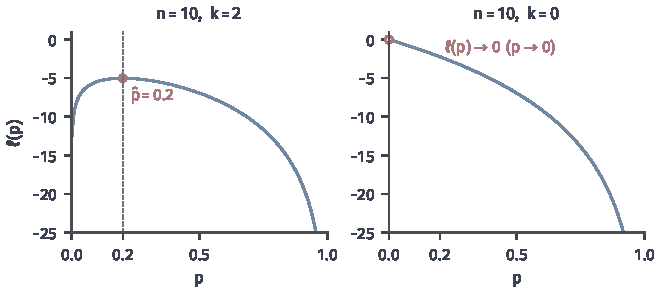
\includegraphics[width=112mm]{figures/01-basic-mathematics/05-probability-and-statistics-basics/matplotlib/est-bernoulli-loglik/figure.pdf}
  \caption{$10$次Bernoulli观测的对数似然$\ell(p)=k\ln p+(10-k)\ln(1-p)$。左：抽检数据$k=2$，曲线在$\hat p=0.2$处取得内部最大值。右：$10$件全部合格（$k=0$），$\ell(p)=10\ln(1-p)$在$(0,1)$上严格递减，上确界$0$只在端点$p=0$处达到（空心圆）。纵轴在$-25$处截断。}
  \label{fig:est-bernoulli-loglik}
\end{figure}

\paragraph{高斯均值模型}
再看读数数据，先假定测量方差已知，只估计均值。这时对数似然中依赖参数的部分是一个平方和，用配方比求导更直接。

\begin{example}[已知方差时高斯均值的最大似然估计]
\label{ex:est-mle-gaussian-mean}
设$X_i\sim\mathcal{N}(\mu,\sigma^2)$，$\sigma^2$已知，只估计$\mu$。由高斯密度$f(x;\mu)=\frac{1}{\sqrt{2\pi}\sigma}\exp\!\big(-\frac{(x-\mu)^2}{2\sigma^2}\big)$，
\[
\ell(\mu)=-\frac n2\ln(2\pi\sigma^2)-\frac{1}{2\sigma^2}\sum_{i=1}^n(x_i-\mu)^2 .
\]
第一项与$\mu$无关，所以最大化$\ell$等价于最小化平方和$\sum_i(x_i-\mu)^2$。利用与式~\eqref{eq:est-sum-of-squares-decomposition}相同的分解，$\sum_i(x_i-\mu)^2=\sum_i(x_i-\bar x)^2+n(\bar x-\mu)^2$，第二项在$\mu=\bar x$时为零、其余时候为正，因此$\hat\mu=\bar x$，无需求导。对读数数据，$\hat\mu=10.1$。高斯误差下的最大似然因而化为最小二乘，这一联系在第~\ref{chap:linear-equations-and-optimization}章的最小二乘问题中还会以向量形式出现。
\end{example}

\paragraph{均值与方差都未知}
现在把均值和方差同时作为参数。为了求导方便，把方差记作$v=\sigma^2>0$。记$\mathrm{SS}(\mu)=\sum_i(x_i-\mu)^2$，对数似然为
\[
\ell(\mu,v)=-\frac n2\ln(2\pi)-\frac n2\ln v-\frac{\mathrm{SS}(\mu)}{2v},\qquad \mu\in\mathbb{R},\ v>0 .
\]
我们分两步求最大值。第一步，固定任意$v>0$，$\ell$作为$\mu$的函数在$\mu=\bar x$处最大，理由同上例。所以对每个$v$都有$\ell(\mu,v)\le\ell(\bar x,v)$。第二步，记$\mathrm{SS}=\mathrm{SS}(\bar x)=\sum_i(x_i-\bar x)^2$，并假定$\mathrm{SS}>0$，即观测不全相同。考虑一元函数
\[
g(v)=\ell(\bar x,v)=-\frac n2\ln(2\pi)-\frac n2\ln v-\frac{\mathrm{SS}}{2v},\qquad
g'(v)=-\frac{n}{2v}+\frac{\mathrm{SS}}{2v^2}=\frac{\mathrm{SS}-nv}{2v^2}.
\]
$g'(v)$在$v<\mathrm{SS}/n$时为正，在$v>\mathrm{SS}/n$时为负，所以$g$在$v=\mathrm{SS}/n$处取最大值。合并两步，最大似然估计为
\begin{equation}
\label{eq:est-mle-gaussian}
\hat\mu=\bar x,\qquad
\hat\sigma^2=\frac1n\sum_{i=1}^n(x_i-\bar x)^2 .
\end{equation}

\begin{example}[读数的最大似然估计]
\label{ex:est-mle-readings}
对读数数据，$\hat\mu=10.1$，$\hat\sigma^2=0.28/8=0.035$，$\hat\sigma\approx0.187$。图~\ref{fig:est-gaussian-contours}画出对数似然在$(\mu,\sigma)$平面上的等高线：等高线围绕最大值点呈封闭的卵形，在$\sigma$方向上不对称，下方（$\sigma$较小）排列更密，说明把$\sigma$估小比估大使似然下降得更快。
\end{example}

\begin{figure}[htbp]
  \centering
  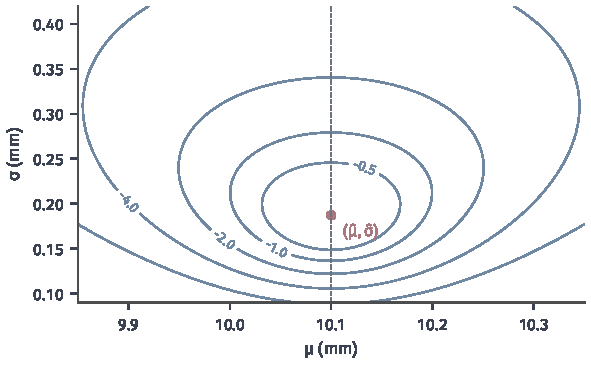
\includegraphics[width=100mm]{figures/01-basic-mathematics/05-probability-and-statistics-basics/matplotlib/est-gaussian-contours/figure.pdf}
  \caption{$8$个读数在高斯模型下的对数似然等高线，以$(\mu,\sigma)$为坐标。各等高线标注的是与最大值之差，由内向外依次为$-0.5,-1,-2,-4,-8$（最外一条未标注）。红点为最大似然估计$(\hat\mu,\hat\sigma)=(10.1,0.187)$，虚线$\mu=\bar x$上各点是固定$\sigma$时对$\mu$的最优选择。}
  \label{fig:est-gaussian-contours}
\end{figure}

把式~\eqref{eq:est-mle-gaussian}与前面的结果放在一起比较：方差的最大似然估计与矩估计~\eqref{eq:est-mom-gaussian}相同，分母都是$n$，而修正样本方差的分母是$n-1$。最大似然估计的分母为$n$，是因为它要使当前数据的似然最大；在$\mu$取$\bar x$之后，对数似然对$v$的最优点恰好是平方离差的平均。它并不以“期望等于$\sigma^2$”为目标，所以与定理~\ref{thm:est-sample-variance-expectation}给出的修正因子无关。两种分母代表两种不同的构造原则，而不是一对一错。

\subsection{边界解与解的存在性}

上面的例子中，最大值都在参数集内部取得，令导数为零就找到了它。本小节说明，这一做法可能失效：最大值可能落在边界上，也可能根本不存在。

\paragraph{边界上的最大值}
Bernoulli的推导假定了$0<k<n$。若抽检中一件不合格品都没有出现，导数就不再有零点。

\begin{example}[全部合格]
\label{ex:est-mle-boundary}
若抽检的$10$件产品全部合格，即$k=0$，则$L(p)=(1-p)^{10}$，$\ell(p)=10\ln(1-p)$。对$p\in(0,1)$，$\ell'(p)=-\frac{10}{1-p}<0$，导数在内部没有零点，对数似然严格递减（图~\ref{fig:est-bernoulli-loglik}右）。

结论取决于参数集。若$\Theta=[0,1]$，$L$在端点$p=0$处取得最大值$L(0)=1$，最大似然估计为$\hat p=0$。若出于“不合格率不可能恰为$0$”的考虑把参数集取为$(0,1)$，则对每个$p\in(0,1)$，都有更小的$p'$使$L(p')>L(p)$；$\sup_{0<p<1}L(p)=1$，但没有任何参数达到它，最大似然估计不存在。同样的讨论适用于全部不合格的情形$k=n$。
\end{example}

全部合格时给出$\hat p=0$，意味着“认为这条生产线永远不会出次品”，只凭$10$件产品显然不足以下这样的结论。这个问题来自数据太少，而不是计算错误；第~\ref{sec:est-bayes}节的后验估计会给出一种在内部取值的替代。

\paragraph{似然无界}
高斯模型的推导在第二步假定了$\mathrm{SS}>0$。如果所有观测都相同，情况完全不同。

\begin{example}[全部观测相同]
\label{ex:est-mle-unbounded}
设$3$次读数都是$10.0$。取$\mu=10.0$，则$\mathrm{SS}(\mu)=0$，对数似然化为
\[
\ell(10.0,\sigma)=-3\ln\sigma-\frac32\ln(2\pi).
\]
当$\sigma\to0^+$时，它趋于$+\infty$。似然在$\mu\in\mathbb{R}$、$\sigma>0$上没有上界，因此不存在最大似然估计。形式上代入式~\eqref{eq:est-mle-gaussian}会得到$\hat\sigma^2=0$，但它不在参数集$(0,\infty)$中，不是任何高斯分布的方差。
\end{example}

图~\ref{fig:est-unbounded-likelihood}把这一情形与读数互不相同的样本对照。观测略有差异时，$\mathrm{SS}>0$使$-\mathrm{SS}/(2\sigma^2)$在$\sigma\to0$时趋于$-\infty$，压过了$-n\ln\sigma$的增长，曲线在内部出现最大值；观测完全相同时，前一项消失，只剩下无限增长的$-n\ln\sigma$。对连续模型，样本中出现完全相同的值往往是仪器分辨率有限、数据被取整的结果，此时应当重新考虑模型是否恰当。

\begin{figure}[htbp]
  \centering
  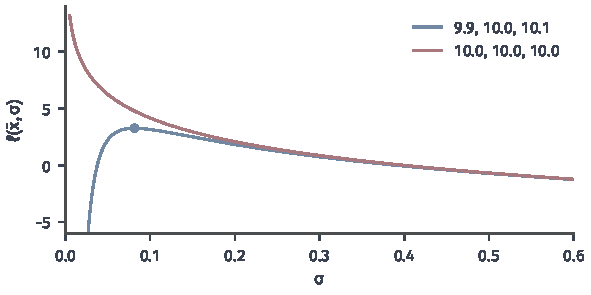
\includegraphics[width=100mm]{figures/01-basic-mathematics/05-probability-and-statistics-basics/matplotlib/est-unbounded-likelihood/figure.pdf}
  \caption{取$\mu=\bar x$时高斯对数似然随$\sigma$的变化。蓝线：读数$9.9,10.0,10.1$，曲线在$\hat\sigma=\sqrt{0.02/3}\approx0.082$处取得最大值（圆点）。红线：三个读数都等于$10.0$，平方离差和为零，对数似然$-3\ln\sigma-\frac32\ln(2\pi)$在$\sigma\to0$时无限增大，最大值不存在。纵轴在$14$处截断。}
  \label{fig:est-unbounded-likelihood}
\end{figure}

\paragraph{最大值、上确界与无界}
两个例子提示我们区分三种情形：似然在参数集中取得最大值，最大似然估计存在；似然有上确界但不被任何参数取到，如参数集为$(0,1)$时的全部合格数据；似然无上界，如全部观测相同的高斯数据。令导数为零只能找出参数集内部的候选点，不能区分这三种情形。完整的计算必须检查参数集的边界，以及参数趋于边界或无穷远时似然的走向。

\section{基于先验与后验的估计}
\label{sec:est-bayes}

矩估计和最大似然估计都只使用当前数据。实际问题中，我们在看到数据之前往往已经对参数有所了解：同类生产线的不合格率通常在$10\%$左右，或者仪器的标称长度是$10.0$mm。本节用概率分布表示这种了解，再用Bayes公式把它与数据合并，最后从合并后的分布中提取估计。

\subsection{先验分布}

\paragraph{参数的不确定性}
前几节把参数看作未知的常数。现在我们换一个角度：既然不知道$\theta$，就用一个概率分布描述“$\theta$可能在哪里，各处的可能性有多大”。这个分布描述的是我们对参数的认识程度，而不是参数自身在随机变化。

\begin{definition}[先验分布]
\label{def:est-prior}
在统计模型$\{F_\theta:\theta\in\Theta\}$中，把参数看作取值于$\Theta$的随机变量，并给定它的分布$\pi(\theta)$（质量函数或密度），称为\term{先验分布}（prior distribution）。观测模型$p(x\mid\theta)$或$f(x\mid\theta)$表示给定参数后数据的条件分布。先验分布中用于调节位置和形状的常数称为\term{超参数}（hyperparameter）。
\end{definition}

于是有两层分布：先验$\pi(\theta)$描述参数的不确定性；观测模型描述参数给定后，个体观测的随机性。这正对应第~\ref{sec:est-samples}节区分的两种不确定性。先验的取值范围必须与参数集一致，例如不合格率的先验只能放在$[0,1]$上；在独立同分布模型中，给定$\theta$后各观测条件独立，联合条件密度仍是式~\eqref{eq:est-sample-joint}的乘积。

\paragraph{Beta先验}
不合格率$p$取值于$[0,1]$，需要一个支撑在$[0,1]$上、形状灵活的分布。第~\ref{sec:prob-beta}节介绍的Beta分布正好合适，其密度为
\[
\pi(p)=\frac{p^{a-1}(1-p)^{b-1}}{B(a,b)},\qquad 0<p<1,
\]
其中$a,b>0$是超参数，$B(a,b)=\int_0^1t^{a-1}(1-t)^{b-1}\mathrm{d}t$是归一化常数。它的均值为$\frac{a}{a+b}$；$a,b>1$时众数为$\frac{a-1}{a+b-2}$。均值决定分布的位置，和$a+b$决定集中程度：均值固定时，$a+b$越大，分布越集中在均值附近。

\begin{example}[两个Beta先验]
\label{ex:est-beta-priors}
若对不合格率没有特别的倾向，可以取$\operatorname{Beta}(1,1)$，即$[0,1]$上的均匀分布。若同类生产线的经验表明不合格率约为$10\%$，可以取$\operatorname{Beta}(2,18)$：均值为$2/20=0.1$，众数为$1/18\approx0.056$，大部分概率集中在$0.3$以下。图~\ref{fig:est-beta-updating}中的灰色虚线就是这两个先验。
\end{example}

\paragraph{高斯先验}
对读数的均值$\mu$，假定仪器的测量标准差$\sigma=0.2$mm已经标定，只有$\mu$未知。$\mu$可以取任何实数，常用高斯先验
\[
\mu\sim\mathcal{N}(m_0,\tau_0^2),
\]
超参数$m_0$表示先验中心，$\tau_0$表示我们对这个中心有多大把握：$\tau_0$越小，先验越集中。例如零件的标称长度为$10.0$mm，加工误差通常在$\pm0.2$mm之内，可以取$m_0=10.0$，$\tau_0=0.1$，使$\mu$约有$95\%$的先验概率落在$10.0\pm0.2$之中。

\subsection{后验分布的计算}
\label{sec:est-posterior}

\paragraph{Bayes公式}
看到数据之后，我们要更新对参数的认识，即求给定数据时参数的条件分布。第~\ref{sec:rvec-bayes-formula}节的Bayes公式对密度同样成立：条件密度等于联合密度除以边缘密度，而联合密度等于先验乘以观测模型。

\begin{definition}[后验分布]
\label{def:est-posterior}
给定先验$\pi(\theta)$与观测数据$x=(x_1,\dots,x_n)$，参数的条件分布
\begin{equation}
\label{eq:est-bayes}
\pi(\theta\mid x)=\frac{f(x\mid\theta)\,\pi(\theta)}{\int_\Theta f(x\mid\vartheta)\,\pi(\vartheta)\,\mathrm{d}\vartheta}
\end{equation}
称为\term{后验分布}（posterior distribution），其中分母是使后验积分为$1$的常数，不依赖$\theta$。观测离散时把$f$换成质量函数$p$；参数取有限个值时，分母中的积分换成求和，$\pi$换成质量函数。
\end{definition}

分子中的$f(x\mid\theta)$作为$\theta$的函数正是似然$L(\theta)$。由于分母只是常数，计算时常写成
\[
\pi(\theta\mid x)\propto L(\theta)\,\pi(\theta),
\]
意思是两边作为$\theta$的函数只差一个正常数因子。实际做法是：先把先验与似然相乘，只保留依赖$\theta$的部分，认出它是哪个分布的密度形状，最后由该分布读出归一化常数。

\paragraph{Beta--Bernoulli模型}
设先验为$p\sim\operatorname{Beta}(a,b)$，在$n$次独立Bernoulli观测中有$k$次取值$1$。似然为$p^k(1-p)^{n-k}$，于是
\[
\pi(p\mid x)\propto p^k(1-p)^{n-k}\cdot p^{a-1}(1-p)^{b-1}=p^{a+k-1}(1-p)^{b+n-k-1},\qquad 0<p<1 .
\]
右边正是Beta密度的形状，所以后验为
\begin{equation}
\label{eq:est-beta-posterior}
p\mid x\ \sim\ \operatorname{Beta}(a+k,\ b+n-k) .
\end{equation}
更新规则非常简单：每观察到一次“$1$”，第一个参数加$1$；每观察到一次“$0$”，第二个参数加$1$。因此先验参数$a,b$可以理解为“先验中相当于已经看到的$a$次$1$与$b$次$0$”，只是$a,b$不必是整数。后验的均值可以写成先验均值与样本比例的加权平均：
\begin{equation}
\label{eq:est-beta-posterior-mean}
\frac{a+k}{a+b+n}=\frac{a+b}{a+b+n}\cdot\frac{a}{a+b}+\frac{n}{a+b+n}\cdot\frac{k}{n},
\end{equation}
两个权重分别与先验“等效样本量”$a+b$和真实样本量$n$成比例。

\begin{example}[抽检数据的后验]
\label{ex:est-beta-posterior}
抽检数据有$n=10$，$k=2$。在均匀先验$\operatorname{Beta}(1,1)$下，后验为$\operatorname{Beta}(3,9)$，后验均值$3/12=0.25$。在先验$\operatorname{Beta}(2,18)$下，后验为$\operatorname{Beta}(4,26)$，后验均值$4/30\approx0.133$；按式~\eqref{eq:est-beta-posterior-mean}，它等于$\frac{20}{30}\times0.1+\frac{10}{30}\times0.2$，先验的权重是数据的两倍，因为先验相当于$20$次观测，而数据只有$10$次。
\end{example}

图~\ref{fig:est-beta-updating}比较了两种先验下的更新。均匀先验在$[0,1]$上是常数，后验与归一化的似然完全重合，数据单独决定后验形状；集中的先验则把后验拉向$0.1$，后验位于先验与似然之间，并且比两者都更集中。

\begin{figure}[htbp]
  \centering
  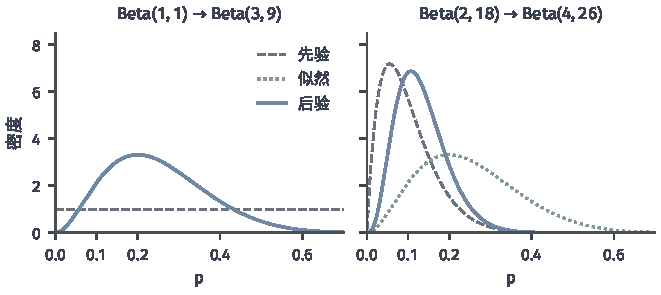
\includegraphics[width=112mm]{figures/01-basic-mathematics/05-probability-and-statistics-basics/matplotlib/est-beta-updating/figure.pdf}
  \caption{抽检数据（$10$件中$2$件不合格）对两种Beta先验的更新。灰色虚线为先验，绿色点线为归一化后的似然$p^2(1-p)^8\times495$，蓝色实线为后验。左：均匀先验$\operatorname{Beta}(1,1)$，后验$\operatorname{Beta}(3,9)$与归一化似然重合。右：先验$\operatorname{Beta}(2,18)$，后验$\operatorname{Beta}(4,26)$介于先验与似然之间。}
  \label{fig:est-beta-updating}
\end{figure}

\paragraph{已知方差的高斯均值模型}
设$\sigma^2$已知，先验$\mu\sim\mathcal{N}(m_0,\tau_0^2)$，观测$x_1,\dots,x_n$在给定$\mu$时独立同分布于$\mathcal{N}(\mu,\sigma^2)$。由例~\ref{ex:est-mle-gaussian-mean}中的平方和分解，似然中依赖$\mu$的部分为$\exp\!\big(-\frac{n(\mu-\bar x)^2}{2\sigma^2}\big)$。乘以先验密度中依赖$\mu$的部分，
\[
\pi(\mu\mid x)\propto\exp\!\Big(-\frac{n(\mu-\bar x)^2}{2\sigma^2}-\frac{(\mu-m_0)^2}{2\tau_0^2}\Big).
\]
为了看出这是什么分布，我们把指数中关于$\mu$的二次式配方。记
\[
\frac{1}{\tau_n^2}=\frac{1}{\tau_0^2}+\frac{n}{\sigma^2},\qquad
m_n=\tau_n^2\Big(\frac{m_0}{\tau_0^2}+\frac{n\bar x}{\sigma^2}\Big).
\]
展开指数中的两个平方，$\mu^2$的系数为$-\frac12\big(\frac{n}{\sigma^2}+\frac1{\tau_0^2}\big)=-\frac{1}{2\tau_n^2}$，$\mu$的系数为$\frac{n\bar x}{\sigma^2}+\frac{m_0}{\tau_0^2}=\frac{m_n}{\tau_n^2}$。因此指数等于$-\frac{\mu^2-2m_n\mu}{2\tau_n^2}$加上一个与$\mu$无关的常数，也就是$-\frac{(\mu-m_n)^2}{2\tau_n^2}$加上常数。常数并入比例因子，得到后验
\begin{equation}
\label{eq:est-gaussian-posterior}
\mu\mid x\ \sim\ \mathcal{N}(m_n,\tau_n^2),\qquad
\frac{1}{\tau_n^2}=\frac{1}{\tau_0^2}+\frac{n}{\sigma^2},\qquad
m_n=\frac{\frac{1}{\tau_0^2}m_0+\frac{n}{\sigma^2}\bar x}{\frac{1}{\tau_0^2}+\frac{n}{\sigma^2}} .
\end{equation}

方差的倒数称为\term{精度}（precision），它度量分布的集中程度。式~\eqref{eq:est-gaussian-posterior}表明两件事。第一，后验精度等于先验精度$1/\tau_0^2$与数据精度$n/\sigma^2$之和，每增加一个观测，精度增加$1/\sigma^2$，所以后验总比先验集中，且随$n$增大越来越集中。第二，后验均值是先验中心$m_0$与样本均值$\bar x$的加权平均，权重与各自的精度成比例：先验越集中，越靠近$m_0$；数据越多或测量越精确，越靠近$\bar x$。

\begin{example}[读数的后验]
\label{ex:est-gaussian-posterior}
取$\sigma=0.2$，先验$\mathcal{N}(10.0,0.1^2)$，数据$n=8$，$\bar x=10.1$。先验精度为$1/0.01=100$，数据精度为$8/0.04=200$，后验精度为$300$，所以$\tau_n^2=1/300$，$\tau_n\approx0.0577$。后验均值
\[
m_n=\frac{100\times10.0+200\times10.1}{300}=\frac{3020}{300}\approx10.067 .
\]
数据的精度是先验的两倍，所以后验均值位于$10.0$与$10.1$之间、离$10.1$更近的三分之二处。
\end{example}

图~\ref{fig:est-gaussian-posterior}画出了这三条曲线。似然曲线以$\bar x=10.1$为中心，标准差为$\sigma/\sqrt n\approx0.071$；先验以$10.0$为中心，标准差为$0.1$；后验中心在两者之间，宽度比两者都窄。

\begin{figure}[htbp]
  \centering
  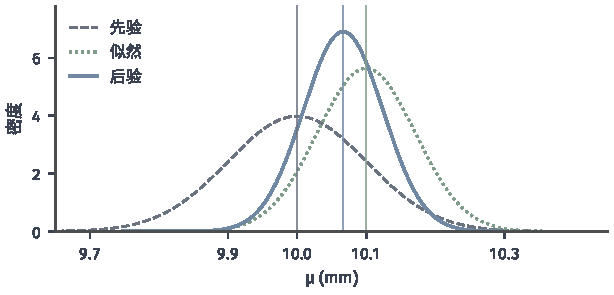
\includegraphics[width=104mm]{figures/01-basic-mathematics/05-probability-and-statistics-basics/matplotlib/est-gaussian-posterior/figure.pdf}
  \caption{已知$\sigma=0.2$时读数均值$\mu$的更新。灰色虚线为先验$\mathcal{N}(10.0,0.1^2)$；绿色点线为归一化的似然，即以$\bar x=10.1$为中心、标准差$0.2/\sqrt8$的高斯曲线；蓝色实线为后验$\mathcal{N}(10.067,1/300)$。三条竖线依次标出$10.0$、$10.067$与$10.1$。}
  \label{fig:est-gaussian-posterior}
\end{figure}

\paragraph{共轭性的含义}
两个例子有一个共同点：先验与后验属于同一个分布族，更新只改变超参数。Beta先验配Bernoulli观测得到Beta后验；高斯先验配已知方差的高斯观测得到高斯后验。

\begin{definition}[共轭先验]
\label{def:est-conjugate-prior}
设$\mathcal{P}$是参数集上的一族分布。若对$\mathcal{P}$中的任一先验和任意观测数据，按式~\eqref{eq:est-bayes}得到的后验仍属于$\mathcal{P}$，则称$\mathcal{P}$是该观测模型的\term{共轭先验}（conjugate prior）族。
\end{definition}

共轭性的计算意义在于：后验不需要数值积分，只需按公式~\eqref{eq:est-beta-posterior}或~\eqref{eq:est-gaussian-posterior}更新几个数。它还使分批处理数据十分方便：先用前一批数据得到后验，再把它当作下一批数据的先验，结果与一次处理全部数据相同。例如抽检数据若分两批，前$5$件含$1$件不合格、后$5$件含$1$件不合格，均匀先验先更新为$\operatorname{Beta}(2,5)$，再更新为$\operatorname{Beta}(3,9)$，与一次更新的结果一致。非共轭的模型中，式~\eqref{eq:est-bayes}的分母通常没有闭式，需要数值方法计算。第~\ref{chap:intervals-tests-prediction}章将用这里的两个后验构造可信区间并预测新观测。

\subsection{后验点估计}

\paragraph{三种常用的点估计}
后验分布完整地描述了看到数据后我们对参数的认识。但很多时候需要报告一个数，例如“不合格率估计为多少”。从后验中提取一个代表值，常用的有三种：
\begin{itemize}
  \item \term{后验均值}（posterior mean）$\mathbb{E}[\theta\mid x]=\int_\Theta\theta\,\pi(\theta\mid x)\,\mathrm{d}\theta$；
  \item \term{后验中位数}（posterior median），即满足$\mathbb{P}(\theta\le a\mid x)=1/2$的$a$；
  \item 后验众数，即后验密度的最大值点，也称\term{最大后验估计}（maximum a posteriori estimate，MAP）。
\end{itemize}
三者分别对应后验分布的“平均位置”“对半分的位置”和“最可能的位置”。前两者可以从另一个角度理解：如果用数$a$去报告$\theta$，并按某种方式衡量报告误差，那么它们分别使不同误差的后验平均最小。

\begin{theorem}[后验均值与后验中位数的最优性]
\label{thm:est-posterior-mean-median}
设后验分布有密度，且$\mathbb{E}[\theta^2\mid x]<\infty$。
\begin{enumerate}
  \item 函数$a\mapsto\mathbb{E}[(\theta-a)^2\mid x]$在$a=\mathbb{E}[\theta\mid x]$处取得唯一最小值。
  \item 记后验分布函数为$G(a)=\mathbb{P}(\theta\le a\mid x)$，并设其密度连续。若$G(a^\ast)=1/2$，则函数$a\mapsto\mathbb{E}[|\theta-a|\mid x]$在$a^\ast$处取得最小值。
\end{enumerate}
\end{theorem}

\begin{proof}
（1）记$\bar\theta=\mathbb{E}[\theta\mid x]$。把$\theta-a$写成$(\theta-\bar\theta)+(\bar\theta-a)$，展开平方并取后验期望，交叉项$2(\bar\theta-a)\mathbb{E}[\theta-\bar\theta\mid x]=0$，于是
\[
\mathbb{E}[(\theta-a)^2\mid x]=\operatorname{Var}(\theta\mid x)+(\bar\theta-a)^2 .
\]
第一项不依赖$a$，第二项在$a=\bar\theta$时为零、其余时候为正。

（2）记后验密度为$g$，则
\[
h(a)=\mathbb{E}[|\theta-a|\mid x]=\int_{-\infty}^a(a-\theta)g(\theta)\,\mathrm{d}\theta+\int_a^{\infty}(\theta-a)g(\theta)\,\mathrm{d}\theta .
\]
按积分上下限求导（第~\ref{chap:univariate-integration}章），两个积分的边界项在$\theta=a$处都为零，得
\[
h'(a)=\int_{-\infty}^a g(\theta)\,\mathrm{d}\theta-\int_a^{\infty}g(\theta)\,\mathrm{d}\theta=2G(a)-1 .
\]
$G$不减，所以$h'(a)$在$a<a^\ast$时不大于$0$，在$a>a^\ast$时不小于$0$；$h$在$a^\ast$左侧不增、右侧不减，故在$a^\ast$处取得最小值。
\end{proof}

因此，若报告误差按平方计，应报告后验均值；若按绝对值计，应报告后验中位数。后验众数没有类似的平方或绝对误差解释，它的含义是“后验密度最高的位置”。当先验是均匀分布时，后验密度与似然成比例，后验众数就是最大似然估计。

\paragraph{Beta后验的点估计}
对后验$\operatorname{Beta}(a',b')$，其中$a'=a+k$，$b'=b+n-k$，后验均值为$\frac{a'}{a'+b'}$。后验众数需要分情况：$a',b'>1$时密度在内部有唯一最大值点$\frac{a'-1}{a'+b'-2}$；$a'\le1$或$b'\le1$时，密度在内部没有极大值点：例如$a'=1<b'$时，密度$b'(1-p)^{b'-1}$在端点$p=0$处最大；$a'<1$时，密度在$p\to0$时无界，众数不存在；$a'=b'=1$时密度为常数，每一点都是众数。后验中位数没有初等闭式，需要数值计算。

\begin{example}[抽检数据的三种后验估计]
\label{ex:est-beta-point-estimates}
在均匀先验下，后验为$\operatorname{Beta}(3,9)$：后验均值为$3/12=0.25$，后验众数为$2/10=0.2$，数值计算得后验中位数约为$0.236$。众数等于最大似然估计$0.2$，这正是均匀先验下两者一致的体现。图~\ref{fig:est-posterior-summaries}显示，这个后验向右偏斜，右侧的长尾把均值拉到中位数右侧，众数则在三者中最小。

在先验$\operatorname{Beta}(2,18)$下，后验为$\operatorname{Beta}(4,26)$，均值约为$0.133$，众数为$3/28\approx0.107$，中位数约为$0.125$，三者都小于样本比例$0.2$，反映了先验的影响。

若$10$件全部合格，均匀先验下的后验为$\operatorname{Beta}(1,11)$，其密度$11(1-p)^{10}$在$p=0$处最大，所以后验众数为$0$，与最大似然估计相同；但后验均值为$1/12\approx0.083$，后验中位数为$1-2^{-1/11}\approx0.061$，二者都在$(0,1)$内部。与例~\ref{ex:est-mle-boundary}中的$\hat p=0$相比，它们避免了“永不出次品”的结论。
\end{example}

\begin{figure}[htbp]
  \centering
  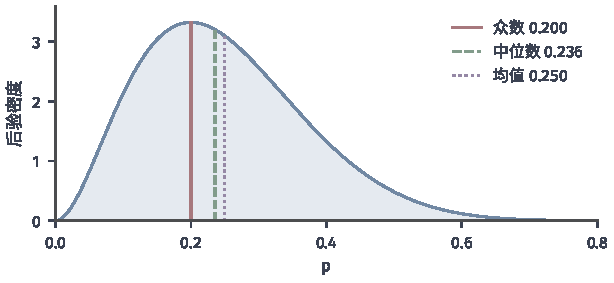
\includegraphics[width=104mm]{figures/01-basic-mathematics/05-probability-and-statistics-basics/matplotlib/est-posterior-summaries/figure.pdf}
  \caption{偏斜的后验$\operatorname{Beta}(3,9)$上三种点估计的位置。红色实线为后验众数$0.2$，绿色虚线为后验中位数约$0.236$，紫色点线为后验均值$0.25$。分布的右尾较长，使均值位于中位数右侧。}
  \label{fig:est-posterior-summaries}
\end{figure}

\paragraph{对称后验与存在性}
对高斯后验$\mathcal{N}(m_n,\tau_n^2)$，密度关于$m_n$对称且在$m_n$处唯一取得最大值，所以后验均值、中位数和众数都等于$m_n$。对读数数据，三者都约为$10.067$。

一般情况下，三种点估计的存在性和唯一性都不能一概假定。后验均值要求后验期望存在；中位数可能在一个区间上都满足$G(a)=1/2$，此时不唯一；众数可能不唯一，也可能不存在。例如后验$\operatorname{Beta}(0.5,0.5)$的密度在$p\to0$和$p\to1$时都趋于无穷，没有最大值点，而它的均值和中位数都是$0.5$，恰好位于密度最低的地方。报告后验点估计时，最好同时查看后验分布的形状。

\section{本章小结}
\label{sec:est-summary}

本章从“由有限数据了解总体规律”这一问题出发，建立了一条对象链：总体规律由统计模型$\{F_\theta:\theta\in\Theta\}$表示；随机样本$X_1,\dots,X_n$是独立同分布的随机变量，其联合分布由式~\eqref{eq:est-sample-joint}的乘积给出；统计量是不含未知参数的样本函数，用于估计时称为估计量，代入数据后得到估计值。独立同分布是对抽样方式的假设，不放回抽样和时间序列等情形需要另行检查。

在不假定模型时，经验分布把概率$1/n$放在每个观测上，经验分布函数、样本矩、样本方差和样本分位数都是它的数值特征。修正样本方差的分母$n-1$来自平方离差和的期望$(n-1)\sigma^2$；样本分位数在跳跃处有多种约定，小样本时需要说明所用的约定。

三类估计使用了不同的信息。矩估计只使用几个样本矩，计算简单，但要检查矩是否存在、能否确定参数、解是否落在参数集中并与数据相容。最大似然估计使用模型的整个联合分布，在常见模型中化为求导和配方，但令导数为零不能代替对边界解和无界似然的检查。基于后验的估计额外使用先验信息，Bayes公式把先验与似然合并为后验；在Beta--Bernoulli和已知方差的高斯均值这两个共轭模型中，后验均值都是先验中心与样本均值的加权平均，权重由先验的等效样本量或精度决定。从后验中提取均值、中位数和众数，分别对应平方误差、绝对误差和密度最高这三种标准。

用全章的两组数据比较：不合格率的矩估计和最大似然估计都是$0.2$，均匀先验下后验均值为$0.25$、后验众数为$0.2$；读数均值的三种估计依次为$10.1$、$10.1$与$10.067$，方差的矩估计和最大似然估计都是$0.035$，修正样本方差为$0.04$。同一个参数有多个估计，它们在当前数据上给出不同的数，单凭一组数据无法判断哪一个更接近真值。要比较它们，就要回到抽样之前，研究估计量作为随机变量的分布：它的中心在哪里，波动有多大，样本量增加时如何变化。这正是第~\ref{chap:sampling-errors}章的内容。

\chapter{抽样分布与估计误差}
\label{chap:sampling-errors}

第~\ref{chap:sample-estimation}章从一组观测出发构造了估计：用样本比例估计不合格率，用样本均值估计测量均值，用修正样本方差估计波动大小。
设想我们随机检查了$80$件产品，发现$24$件不合格，于是报告不合格率约为$0.3$。
这个数字离真实不合格率有多远？如果明天换一批$80$件重新检查，报告会变成多少？
再检查$800$件，误差会缩小到什么程度？这些问题都不针对已经算出的那个数，而针对“按同一规则重复抽样、重复计算”时结果的波动。

本章先确定误差的含义。
同一个计算规则在不同样本上给出不同结果，所以统计量本身也有分布；
它的标准差、它的平均位置与目标的距离，以及它到目标的平均平方距离，分别回答“波动多大”“是否系统偏离”“总体上离得多远”。
有了这些指标，我们再研究三类能够说明误差大小的依据。

第一类依据是精确分布：如果总体服从正态分布，样本均值、样本方差及它们的比值都有可以写出的分布，这就是卡方分布、$t$分布与$F$分布的来源。
第二类依据是有限样本概率界：只知道均值或方差时，Markov与Chebyshev不等式仍能对任意固定的样本量给出误差超过阈值的概率上界。
第三类依据是极限定理：样本量增大时，大数定律说明样本均值靠近总体均值，中心极限定理进一步描述放大后的误差近似服从正态分布。
三类依据的条件与结论各不相同，第~\ref{chap:intervals-tests-prediction}章构造区间、检验与预测时会分别用到它们。

\section{抽样分布与误差指标}
\label{sec:samp-errors}

本节固定总体与样本量，把“重复抽样”这个想象中的操作落实成统计量的分布，再用它定义标准误、偏差与均方误差。
这些指标描述的是计算规则的表现，而不是某一次估计值的对错。

\subsection{统计量的抽样分布}

\paragraph{重复抽样下的样本比例}
回到产品检查。设每件产品不合格的概率为$p$，各件是否不合格相互独立，第$i$件的结果记为$X_i\sim\operatorname{Bernoulli}(p)$。
检查$n$件后，不合格件数$S_n=X_1+\dots+X_n$服从$\operatorname{Bin}(n,p)$，样本比例$\hat p=S_n/n$只能取$0,1/n,\dots,1$这些值。
由于$S_n$的分布已经确定，$\hat p$取每个值的概率也随之确定：
\[
  \mathbb{P}\Bigl(\hat p=\frac kn\Bigr)=\mathbb{P}(S_n=k)=\binom nk p^k(1-p)^{n-k},\qquad k=0,1,\dots,n.
\]
这说明样本比例并不是一个固定的数：抽样之前它是随机变量，抽样之后我们只看到它的一个实现。

\begin{example}[样本比例取各值的概率]
\label{ex:samp-proportion-probabilities}
取$p=0.3$，$n=20$。样本比例恰好等于真值$0.3$，即$S_{20}=6$，概率为
\[
  \binom{20}{6}0.3^6\,0.7^{14}\approx0.192.
\]
即使总体比例就是$0.3$，五次重复抽样中也大约只有一次恰好报告$0.3$。
误差不超过$0.1$对应$4\leq S_{20}\leq8$，把五项二项概率相加得到约$0.780$；
换成$n=80$，同一事件对应$16\leq S_{80}\leq32$，概率升到约$0.963$。
样本量增加并没有让$\hat p$变成确定的数，而是让它的分布更集中在真值附近。
\end{example}

图~\ref{fig:samp-sample-proportion}把这一计算与模拟对照。
我们用固定的随机种子重复抽取$10000$组样本，每组算一次$\hat p$，柱高是各取值出现的频率，圆点是上式给出的二项概率。
两者几乎重合，说明“重复抽样得到的频率”与“统计量的分布”是同一件事的经验面和理论面。
比较两个面板还能看到，$n$从$20$增到$80$时，分布的宽度大约缩小一半。

\begin{figure}[htbp]
  \centering
  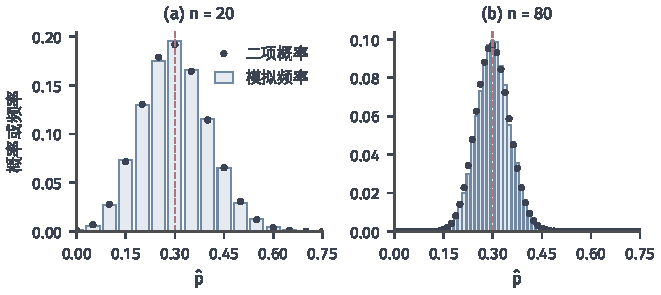
\includegraphics[width=112mm]{figures/01-basic-mathematics/05-probability-and-statistics-basics/matplotlib/samp-sample-proportion/figure.pdf}
  \caption{总体为$\operatorname{Bernoulli}(0.3)$时样本比例$\hat p$的抽样分布。每个面板用固定随机种子重复抽样$10000$次，柱高为$\hat p$各取值出现的频率，圆点为二项分布给出的精确概率，虚线标出真值$0.3$。$n=20$与$n=80$时模拟标准差分别约为$0.102$与$0.051$。}
  \label{fig:samp-sample-proportion}
\end{figure}

\paragraph{抽样分布的定义}
上面的做法对任何统计量都适用。
固定总体分布与样本量$n$后，样本$X_1,\dots,X_n$的联合分布就确定了；统计量$T=t(X_1,\dots,X_n)$是样本的函数，它的分布也随之确定。

\begin{definition}[抽样分布]
\label{def:samp-sampling-distribution}
设样本$X_1,\dots,X_n$来自给定的总体分布，$T=t(X_1,\dots,X_n)$是统计量。
把$T$作为随机变量时的概率分布称为$T$的\term{抽样分布}（sampling distribution）。
\end{definition}

抽样分布依赖三样东西：总体分布、样本量和统计量的计算规则。
总体参数未知时，抽样分布通常也含未知参数；例如$\hat p$的分布依赖$p$。
所以我们往往不能直接画出它，而是研究它的均值、方差或近似形状随参数怎样变化，这正是本章后续各节的任务。

\paragraph{三种分布的区分}
统计中经常同时出现三种“分布”，它们描述的对象不同，混淆会导致错误的结论。
\emph{总体分布}描述单个观测$X_i$的取值规律，例如一件产品是否不合格、一次测量落在哪里；它通常含未知参数。
\emph{经验分布}由一组已经得到的观测构成，第~\ref{sec:est-empirical-cdf}节用经验分布函数$\hat F_n$描述它：每个观测值占$1/n$的质量。
\emph{抽样分布}描述统计量在重复抽样中的取值规律，它的对象既不是单个观测，也不是当前这组数据。

图~\ref{fig:samp-three-distributions}用指数总体把三者放在一起。
左图是总体密度$f(x)=e^{-x}$，单个观测的波动很大，并且明显右偏。
中图是一组$n=25$的观测：经验分布函数是一条阶梯，它围绕总体分布函数随机起伏，这组数据的均值约为$1.15$。
右图把这一步重复$10000$次，统计每次的样本均值：这些均值集中在$1$附近，标准差约为$0.2$，形状也比总体对称得多。
同一个总体、同一个样本量，三幅图回答的问题完全不同。

\begin{figure*}[htbp]
  \centering
  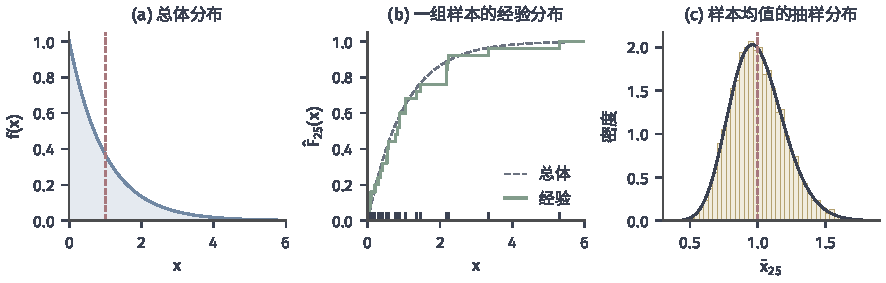
\includegraphics[width=150mm]{figures/01-basic-mathematics/05-probability-and-statistics-basics/matplotlib/samp-three-distributions/figure.pdf}
  \caption{总体分布、经验分布与抽样分布的对照。总体为率参数$1$的指数分布，均值为$1$（虚线）。(a) 总体密度；(b) 一组$n=25$观测的经验分布函数（实线阶梯）与总体分布函数（虚线），底部短线为各观测值；(c) 用固定随机种子重复抽样$10000$次得到的样本均值直方图，实线为其精确密度，即形状$25$、率$25$的Gamma分布。}
  \label{fig:samp-three-distributions}
\end{figure*}

\subsection{标准误}
\label{sec:samp-standard-error}

\paragraph{标准误的定义}
图~\ref{fig:samp-sample-proportion}中两个分布的宽度不同，我们需要一个数来概括“重复抽样时估计值的波动”。
最直接的选择是抽样分布的标准差。

\begin{definition}[标准误]
\label{def:samp-standard-error}
设统计量$T$的方差有限。$T$的抽样分布的标准差$\operatorname{SE}(T)=\sqrt{\operatorname{Var}T}$称为$T$的\term{标准误}（standard error）。
\end{definition}

标准误衡量的是计算规则的稳定性：若用同一规则在许多组独立样本上反复计算，结果大约在其均值附近$\operatorname{SE}(T)$的范围内波动。
它不说明某一次估计值离真值多远，因为单次结果仍可能落在分布的尾部；
它也不包含系统偏离，若$T$的平均位置本身就偏离目标，标准误再小也不能发现，系统偏离要由下一小节的偏差来度量。

\paragraph{样本均值的标准误}
设$X_1,\dots,X_n$独立同分布，均值$\mu$、方差$\sigma^2$有限。
由期望的线性性，$\mathbb{E}\bar X_n=\mu$。
由第~\ref{sec:rvec-moments}节，独立随机变量和的方差等于方差之和，于是
\[
  \operatorname{Var}\bar X_n=\frac1{n^2}\operatorname{Var}\Bigl(\sum_{i=1}^nX_i\Bigr)=\frac1{n^2}\sum_{i=1}^n\operatorname{Var}X_i=\frac{\sigma^2}{n},
\]
从而
\begin{equation}
  \operatorname{SE}(\bar X_n)=\frac{\sigma}{\sqrt n}.
  \label{eq:samp-mean-standard-error}
\end{equation}
这里用到独立性使交叉协方差为零；只假定同分布而观测之间正相关时，均值的方差会更大。
式~\eqref{eq:samp-mean-standard-error}说明误差以$1/\sqrt n$的速度缩小：样本量变为四倍，标准误才减半。
对样本比例，$\sigma^2=p(1-p)$，所以$\operatorname{SE}(\hat p)=\sqrt{p(1-p)/n}$；$p=0.3$时$n=20$与$n=80$分别给出$0.102$与$0.051$，与图~\ref{fig:samp-sample-proportion}的模拟值一致。

\paragraph{数据标准差与均值标准误}
$\sigma$与$\sigma/\sqrt n$描述两个不同对象的波动，不能互相替代。

\begin{example}[称重数据的两种标准差]
\label{ex:samp-weighing-standard-error}
某袋装食品的单袋净重标准差为$\sigma=10$克，随机称量$n=25$袋。
单袋净重的波动约为$10$克，这是数据的标准差，它描述袋与袋之间的差别，不会因为多称几袋而变小。
$25$袋平均净重的标准误是$10/\sqrt{25}=2$克，它描述“若重新抽取$25$袋，平均值会变化多少”，样本量越大越小。
若要把标准误降到$1$克，需要$n=(10/1)^2=100$袋。
\end{example}

实际中$\sigma$通常未知。把样本标准差$S_n$代入，得到\emph{标准误估计}$S_n/\sqrt n$；对比例则常把$\hat p$代入$\sqrt{p(1-p)/n}$。
章首检查$80$件、发现$24$件不合格的例子中，$\hat p=0.3$，标准误估计为$\sqrt{0.3\times0.7/80}\approx0.051$，它告诉读者“若重新检查$80$件，比例大约会在$\pm0.05$的量级上变动”。
标准误估计本身是一个随机量，用它代替$\sigma/\sqrt n$会带来额外误差，第~\ref{sec:samp-t}节和第~\ref{sec:samp-clt}节将分别在正态模型与大样本条件下处理这种替换。

\subsection{偏差}

\paragraph{偏差与无偏性}
标准误只看估计量围绕自身均值的波动。
我们还关心这个均值是否就是要估计的目标：如果一台秤每次都多称$3$克，读数再稳定也不准。
下面用$\mathbb{E}_\theta$表示参数取$\theta$时按样本的联合分布计算期望，以强调期望依赖未知参数。

\begin{definition}[偏差与无偏估计量]
\label{def:samp-bias}
设$\hat\theta$是参数$\theta$的估计量，且对每个$\theta\in\Theta$，$\mathbb{E}_\theta\hat\theta$存在。称
\[
  \operatorname{Bias}_\theta(\hat\theta)=\mathbb{E}_\theta\hat\theta-\theta
\]
为$\hat\theta$在$\theta$处的\term{偏差}（bias）。若对所有$\theta\in\Theta$都有$\operatorname{Bias}_\theta(\hat\theta)=0$，称$\hat\theta$为$\theta$的\term{无偏估计量}（unbiased estimator）。
\end{definition}

无偏性要求对\emph{每一个}可能的参数值都成立，因为我们事先不知道真值是哪一个；只在某个特定$\theta$处偏差为零不算无偏。
无偏性也只说明抽样分布的中心对准目标，不说明单次结果接近真值。
例如只用第一个观测$X_1$估计均值$\mu$，它满足$\mathbb{E}X_1=\mu$，是无偏的，但它的标准误是$\sigma$，不随样本量减小，用$n$个观测时仍然只利用了一个。

\paragraph{样本均值与两种方差估计}
第~\ref{chap:sample-estimation}章已经计算过几个常用统计量的期望，现在把它们放到偏差的框架中。
设$X_1,\dots,X_n$独立同分布，均值$\mu$，方差$\sigma^2$有限，$n\geq2$。

样本均值满足$\mathbb{E}\bar X_n=\mu$，因此是$\mu$的无偏估计量。

对方差，第~\ref{sec:est-sample-variance}节由平方和分解
$\sum_i(X_i-\bar X_n)^2=\sum_i(X_i-\mu)^2-n(\bar X_n-\mu)^2$
求得$\mathbb{E}\sum_i(X_i-\bar X_n)^2=n\sigma^2-\sigma^2=(n-1)\sigma^2$。
于是修正样本方差$S_n^2$满足$\mathbb{E}S_n^2=\sigma^2$，是无偏的；
分母为$n$的$\hat\sigma_n^2=\frac{n-1}{n}S_n^2$满足
\[
  \operatorname{Bias}(\hat\sigma_n^2)=\frac{n-1}{n}\sigma^2-\sigma^2=-\frac{\sigma^2}{n},
\]
平均而言低估了方差。原因是残差$X_i-\bar X_n$以样本均值为中心，而样本均值正是使平方和最小的中心，所以残差平方和系统地小于以真实$\mu$为中心的平方和。

无偏性在非线性变换下一般不保留。样本标准差$S_n=\sqrt{S_n^2}$不是$\sigma$的无偏估计量：由
$0\leq\operatorname{Var}S_n=\mathbb{E}S_n^2-(\mathbb{E}S_n)^2=\sigma^2-(\mathbb{E}S_n)^2$
得$\mathbb{E}S_n\leq\sigma$，只要$S_n$不是常数，不等号就严格成立。

\begin{example}[均匀分布端点的估计]
\label{ex:samp-uniform-maximum-bias}
设$X_1,\dots,X_n$独立同分布于$\operatorname{U}(0,\theta)$，$\theta>0$未知。第~\ref{sec:est-moments}节的矩估计是$2\bar X_n$；最大似然估计则是样本最大值$X_{(n)}$，因为似然在$\theta<X_{(n)}$时为零，在$\theta\geq X_{(n)}$时等于随$\theta$递减的$\theta^{-n}$。
由独立性，对$0\leq x\leq\theta$，
\[
  \mathbb{P}(X_{(n)}\leq x)=\prod_{i=1}^n\mathbb{P}(X_i\leq x)=\Bigl(\frac x\theta\Bigr)^n,
\]
求导得到密度$nx^{n-1}/\theta^n$，于是
\[
  \mathbb{E}X_{(n)}=\int_0^\theta x\cdot\frac{nx^{n-1}}{\theta^n}\,\mathrm{d}x=\frac{n}{n+1}\theta,\qquad
  \operatorname{Bias}_\theta(X_{(n)})=-\frac{\theta}{n+1}.
\]
最大值总落在$\theta$以下，偏差为负是可以预期的。乘上因子得到$\frac{n+1}{n}X_{(n)}$，它是无偏的；
矩估计$2\bar X_n$也是无偏的，因为$\mathbb{E}X_i=\theta/2$。同一个参数有多个无偏估计量，下一小节将说明怎样比较它们。
\end{example}

\subsection{均方误差}
\label{sec:samp-mse}

\paragraph{定义与分解}
标准误和偏差各描述误差的一个方面。为了用一个数衡量估计值离目标总体上有多远，我们取误差平方的平均。

\begin{definition}[均方误差]
\label{def:samp-mse}
设$\mathbb{E}_\theta\hat\theta^2<\infty$。称
\[
  \operatorname{MSE}_\theta(\hat\theta)=\mathbb{E}_\theta\bigl[(\hat\theta-\theta)^2\bigr]
\]
为$\hat\theta$在$\theta$处的\term{均方误差}（mean squared error, MSE）。
\end{definition}

在$\hat\theta-\theta$中加减$\mathbb{E}_\theta\hat\theta$，把误差拆成围绕均值的波动与均值的偏离：
\[
  \hat\theta-\theta=(\hat\theta-\mathbb{E}_\theta\hat\theta)+(\mathbb{E}_\theta\hat\theta-\theta).
\]
平方后取期望，第二项是常数，交叉项为$2(\mathbb{E}_\theta\hat\theta-\theta)\,\mathbb{E}_\theta(\hat\theta-\mathbb{E}_\theta\hat\theta)=0$，于是
\begin{equation}
  \operatorname{MSE}_\theta(\hat\theta)=\operatorname{Var}_\theta\hat\theta+\bigl(\operatorname{Bias}_\theta\hat\theta\bigr)^2.
  \label{eq:samp-mse-decomposition}
\end{equation}
式~\eqref{eq:samp-mse-decomposition}说明，均方误差同时惩罚波动和系统偏离；无偏估计量的均方误差就是方差，即标准误的平方。

\begin{example}[两个无偏估计量与一个有偏估计量]
\label{ex:samp-uniform-mse}
继续示例~\ref{ex:samp-uniform-maximum-bias}。由$\operatorname{Var}X_i=\theta^2/12$，矩估计的均方误差为
$\operatorname{Var}(2\bar X_n)=4\cdot\frac{\theta^2}{12n}=\frac{\theta^2}{3n}$。
对最大值，类似地算出$\mathbb{E}X_{(n)}^2=\frac{n}{n+2}\theta^2$，故
\[
  \operatorname{Var}X_{(n)}=\frac{n\theta^2}{n+2}-\frac{n^2\theta^2}{(n+1)^2}=\frac{n\theta^2}{(n+1)^2(n+2)}.
\]
再加上偏差的平方$\theta^2/(n+1)^2$，
\[
  \operatorname{MSE}(X_{(n)})=\frac{n\theta^2}{(n+1)^2(n+2)}+\frac{\theta^2}{(n+1)^2}=\frac{2\theta^2}{(n+1)(n+2)}.
\]
修正后的$\frac{n+1}{n}X_{(n)}$无偏，均方误差为$\frac{(n+1)^2}{n^2}\operatorname{Var}X_{(n)}=\frac{\theta^2}{n(n+2)}$。
取$n=10$，三者依次约为$0.0333\theta^2$、$0.0152\theta^2$、$0.0083\theta^2$。
两个无偏估计量的均方误差相差四倍；有偏的$X_{(n)}$也明显好于无偏的$2\bar X_n$。
\end{example}

\paragraph{收缩估计中的权衡}
上例中偏差与方差同时变化。下面的例子更直接地说明：主动引入偏差有时能换来更小的均方误差，但这种好处依赖未知参数。

设$X_1,\dots,X_n$独立同分布，均值$\mu$，方差$\sigma^2$已知。考虑把样本均值向$0$拉近的\term{收缩估计量}（shrinkage estimator）$c\bar X_n$，其中常数$0<c<1$。
它的偏差为$(c-1)\mu$，方差为$c^2\sigma^2/n$，所以
\[
  \operatorname{MSE}_\mu(c\bar X_n)=\frac{c^2\sigma^2}{n}+(1-c)^2\mu^2.
\]
与$\operatorname{MSE}(\bar X_n)=\sigma^2/n$相比，第一项变小了，第二项则随$|\mu|$增大而增大。

\begin{example}[收缩估计何时更好]
\label{ex:samp-shrinkage}
取$\sigma^2=1$，$n=10$，$c=0.8$。样本均值的均方误差恒为$0.1$；收缩估计的均方误差为$0.064+0.04\mu^2$。
后者更小当且仅当$0.04\mu^2<0.036$，即$|\mu|<\sqrt{0.9}\approx0.949$。
真值靠近$0$时，收缩带来的方差下降超过偏差代价；真值远离$0$时，偏差平方迅速增长，收缩反而更差。
使均方误差最小的$c$是$\mu^2/(\mu^2+\sigma^2/n)$，它依赖未知的$\mu$，所以不能直接算出。
\end{example}

图~\ref{fig:samp-shrinkage-mse}展示了这一权衡。
左图中$\mu=0.5$，收缩估计的抽样分布更窄，但中心移到了$0.4$；右图显示两条均方误差曲线在$|\mu|\approx0.949$处相交。
没有哪一个估计量对所有参数值都更好，所以比较估计量时必须说明参数范围与误差指标；
只因为一个估计量无偏就选择它，或只因为它方差小就选择它，都没有回答“离真值有多远”这个问题。

\begin{figure}[htbp]
  \centering
  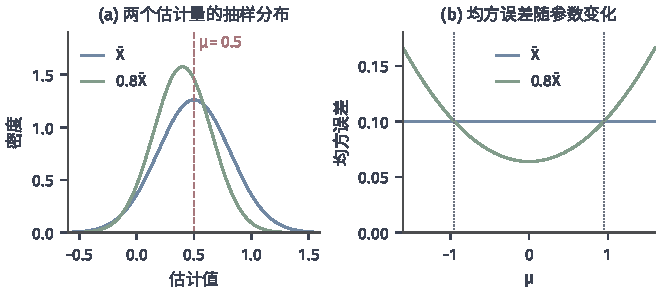
\includegraphics[width=112mm]{figures/01-basic-mathematics/05-probability-and-statistics-basics/matplotlib/samp-shrinkage-mse/figure.pdf}
  \caption{样本均值与收缩估计$0.8\bar X$的比较，总体为$\mathcal N(\mu,1)$，$n=10$。(a) $\mu=0.5$（虚线）时两个估计量的精确抽样密度：收缩估计更窄但中心偏到$0.4$。(b) 均方误差随$\mu$的变化：样本均值恒为$0.1$，收缩估计为$0.064+0.04\mu^2$，点线标出交点$|\mu|\approx0.949$。}
  \label{fig:samp-shrinkage-mse}
\end{figure}

\section{正态样本的精确抽样分布}
\label{sec:samp-normal}

上一节的误差指标只用到均值和方差。要回答“误差超过某个值的概率是多少”，需要整个抽样分布。
一般总体下这个分布很难写出；但当总体服从正态分布时，样本均值、样本方差以及由它们组成的比值都有精确的分布。
本节始终假设$X_1,\dots,X_n$独立同分布于$\mathcal N(\mu,\sigma^2)$，$n\geq2$，并把样本写成向量$\bm X=(X_1,\dots,X_n)^\top$。

\subsection{样本均值与残差}

\paragraph{常数方向上的正交分解}
记$\bm 1=(1,\dots,1)^\top\in\mathbb{R}^n$。样本均值可以写成$\bar X_n=\frac1n\bm 1^\top\bm X$，而
\[
  \bar X_n\bm 1=\frac{\bm 1\bm 1^\top}{n}\bm X
\]
恰是$\bm X$在一维子空间$\operatorname{span}\{\bm 1\}$上的正交投影：$\bm 1/\sqrt n$是该子空间的单位向量，按第~\ref{sec:ls-projection-matrices}节的投影矩阵公式，投影矩阵为$\frac{\bm 1}{\sqrt n}\frac{\bm 1^\top}{\sqrt n}=\bm 1\bm 1^\top/n$。
相应的残差向量$\bm R=\bm X-\bar X_n\bm 1$的分量是$X_i-\bar X_n$，它与$\bm 1$正交，即$\sum_iR_i=0$。
由勾股定理，
\begin{equation}
  \lVert\bm X\rVert_2^2=n\bar X_n^2+\sum_{i=1}^n(X_i-\bar X_n)^2.
  \label{eq:samp-mean-residual-pythagoras}
\end{equation}

两部分记录的信息不同。投影$\bar X_n\bm 1$只告诉我们数据的整体位置，把每个观测都换成同一个数；
残差告诉我们各观测相对这个位置怎样散开，它的平方长度除以$n-1$就是$S_n^2$。
残差受一个线性约束$\sum_iR_i=0$，所以落在$n-1$维的子空间$\{\bm r:\sum_ir_i=0\}$中，这将是后面“$n-1$个自由度”的来源。

\begin{example}[三个观测的分解]
\label{ex:samp-three-point-decomposition}
取一组观测$\bm x=(1,2,6)^\top$。样本均值为$3$，投影为$(3,3,3)^\top$，残差为$(-2,-1,3)^\top$，其分量和为$0$。
式~\eqref{eq:samp-mean-residual-pythagoras}两边分别为$1+4+36=41$与$3\cdot3^2+(4+1+9)=27+14$，相等。
修正样本方差为$14/2=7$。图~\ref{fig:samp-mean-residual-projection}按这组数据的长度画出了分解：横轴代表常数方向，纵轴代表残差所在的子空间。
\end{example}

\begin{figure}[htbp]
  \centering
  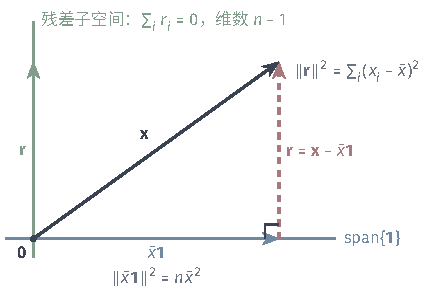
\includegraphics[width=73mm]{figures/01-basic-mathematics/05-probability-and-statistics-basics/tikz/samp-mean-residual-projection/figure.pdf}
  \caption{样本向量的正交分解示意。横轴表示一维常数方向$\operatorname{span}\{\bm 1\}$，纵轴表示$n-1$维残差子空间$\{\bm r:\sum_ir_i=0\}$。样本向量$\bm x$分解为投影$\bar x\bm 1$与残差$\bm r$，两者正交；图中长度取自$\bm x=(1,2,6)^\top$，即$\lVert\bar x\bm 1\rVert^2=27$、$\lVert\bm r\rVert^2=14$。}
  \label{fig:samp-mean-residual-projection}
\end{figure}

\paragraph{零协方差与独立性}
几何上正交并不等于概率上独立。我们先计算两部分的协方差。
由于$\operatorname{Cov}(\bar X_n,X_i)=\frac1n\sum_j\operatorname{Cov}(X_j,X_i)=\frac{\sigma^2}{n}$，
\[
  \operatorname{Cov}(\bar X_n,\,X_i-\bar X_n)=\frac{\sigma^2}{n}-\operatorname{Var}\bar X_n=\frac{\sigma^2}{n}-\frac{\sigma^2}{n}=0,\qquad i=1,\dots,n.
\]
这一计算只用到独立同分布和有限方差，对任何总体都成立。
在正态模型中，$(\bar X_n,\bm R)$是正态向量$\bm X$的线性像，因而联合高斯；第~\ref{sec:rvec-gaussian}节说明，联合高斯的两组分量交叉协方差为零时相互独立。
不过$\bm R$的协方差矩阵是奇异的（它只在$n-1$维子空间中取值），为了只使用非退化的情形，我们换一组正交坐标完成证明。

\begin{theorem}[正态样本的均值与残差]
\label{thm:samp-normal-mean-residual}
设$X_1,\dots,X_n$独立同分布于$\mathcal N(\mu,\sigma^2)$，$n\geq2$。则$\bar X_n\sim\mathcal N(\mu,\sigma^2/n)$，且$\bar X_n$与残差向量$\bm R=\bm X-\bar X_n\bm 1$相互独立。
特别地，$\bar X_n$与$S_n^2=\lVert\bm R\rVert_2^2/(n-1)$相互独立。
\end{theorem}

\begin{proof}
令$Z_i=(X_i-\mu)/\sigma$，则$Z_1,\dots,Z_n$独立同分布于$\mathcal N(0,1)$，$\bm Z$的联合密度为$(2\pi)^{-n/2}e^{-\lVert\bm z\rVert_2^2/2}$。

取$\bm q_1=\bm 1/\sqrt n$，用Gram--Schmidt正交化（定理~\ref{thm:ls-gram-schmidt}）把它扩充为$\mathbb{R}^n$的标准正交基$\bm q_1,\dots,\bm q_n$，以$\bm q_j^\top$为第$j$行组成正交矩阵$\bm Q$，并令$\bm Y=\bm Q\bm Z$。
按第~\ref{sec:rvec-transforms}节的多元变量替换，$\bm Z=\bm Q^\top\bm Y$，Jacobian行列式的绝对值为$|\det\bm Q^\top|=1$，且$\lVert\bm Q^\top\bm y\rVert_2=\lVert\bm y\rVert_2$，所以$\bm Y$的密度为
\[
  f_{\bm Y}(\bm y)=(2\pi)^{-n/2}e^{-\lVert\bm Q^\top\bm y\rVert_2^2/2}=\prod_{j=1}^n\frac1{\sqrt{2\pi}}e^{-y_j^2/2}.
\]
密度分解为乘积，说明$Y_1,\dots,Y_n$相互独立且都服从$\mathcal N(0,1)$。换一种说法：$\bm Y$联合高斯，协方差矩阵$\bm Q\bm Q^\top=\bm I$的非对角元全为零，因而各分量独立。

现在用$\bm Y$表示均值与残差。第一个坐标是
$Y_1=\bm q_1^\top\bm Z=\sqrt n\,\bar Z_n=\sqrt n(\bar X_n-\mu)/\sigma$。
由$\bm Z=\bm Q^\top\bm Y=\sum_jY_j\bm q_j$，且$Y_1\bm q_1=\bar Z_n\bm 1$，得
\[
  \bm Z-\bar Z_n\bm 1=\sum_{j=2}^nY_j\bm q_j,\qquad
  \bm R=\sigma(\bm Z-\bar Z_n\bm 1)=\sigma\sum_{j=2}^nY_j\bm q_j.
\]
于是$\bar X_n=\mu+\sigma Y_1/\sqrt n$只依赖$Y_1$，$\bm R$只依赖$(Y_2,\dots,Y_n)$。独立随机变量的两组不相交分量的函数仍相互独立（第~\ref{sec:rvec-independence}节），所以$\bar X_n$与$\bm R$独立，$S_n^2$作为$\bm R$的函数也与$\bar X_n$独立。最后$Y_1\sim\mathcal N(0,1)$给出$\bar X_n\sim\mathcal N(\mu,\sigma^2/n)$。
\end{proof}

证明中的正交矩阵$\bm Q$只是一次旋转坐标：在新坐标下，第一轴沿常数方向，其余$n-1$轴张成残差子空间。
标准正态向量的密度只依赖长度，旋转后形状不变，各坐标仍然独立；这一点是正态模型特有的。

\begin{example}[非正态总体中均值与方差不独立]
\label{ex:samp-bernoulli-mean-variance-dependent}
设$X_1,X_2$独立同分布于$\operatorname{Bernoulli}(1/2)$。此时$S_2^2=(X_1-X_2)^2/2$。
若$\bar X_2=1/2$，则$X_1\ne X_2$，$S_2^2=1/2$；若$\bar X_2\in\{0,1\}$，则$S_2^2=0$。
知道样本均值就完全确定了样本方差，两者显然不独立，尽管上面的协方差计算仍然给出$\operatorname{Cov}(\bar X_2,X_i-\bar X_2)=0$。
零协方差推出独立，依赖的是正态模型的联合高斯结构。
\end{example}

\subsection{卡方分布与样本方差}
\label{sec:samp-chi-square}

\paragraph{卡方分布的定义}
定理~\ref{thm:samp-normal-mean-residual}的证明把残差的平方长度写成了$\sigma^2\sum_{j=2}^nY_j^2$，即若干独立标准正态变量的平方和。我们先单独研究这类平方和。

\begin{definition}[卡方分布]
\label{def:samp-chi-square}
设$Z_1,\dots,Z_k$独立同分布于$\mathcal N(0,1)$，称$Q=Z_1^2+\dots+Z_k^2$的分布为自由度为$k$的\term{卡方分布}（chi-square distribution），记作$Q\sim\chi^2_k$。正整数$k$称为\term{自由度}（degrees of freedom）。
\end{definition}

自由度就是平方和中独立标准正态项的个数，也可以理解为随机向量$(Z_1,\dots,Z_k)$可以自由变化的方向数，而$Q$是它的平方长度。
由$\mathbb{E}Z_i^2=1$，$\mathbb{E}Q=k$：自由度越大，平方长度平均越大。

\paragraph{与Gamma分布的联系}
先看一项。由第~\ref{sec:prob-univariate-transforms}节平方变换的计算，$Y=Z^2$在$y>0$处的密度为两支逆像$\pm\sqrt y$的贡献之和：
\[
  f_Y(y)=\bigl(\varphi(\sqrt y)+\varphi(-\sqrt y)\bigr)\frac{1}{2\sqrt y}=\frac{1}{\sqrt{2\pi}}y^{-1/2}e^{-y/2}.
\]
与第~\ref{sec:prob-gamma}节的Gamma密度$\frac{\beta^\alpha}{\Gamma(\alpha)}y^{\alpha-1}e^{-\beta y}$比较，这正是$\operatorname{Gamma}(1/2,1/2)$，两者的常数一致也正对应$\Gamma(1/2)=\sqrt\pi$。

再看求和。设$U\sim\operatorname{Gamma}(a,\beta)$与$V\sim\operatorname{Gamma}(b,\beta)$独立，率参数相同。由卷积公式，$U+V$在$y>0$处的密度为
\[
  \int_0^y\frac{\beta^a}{\Gamma(a)}x^{a-1}e^{-\beta x}\,\frac{\beta^b}{\Gamma(b)}(y-x)^{b-1}e^{-\beta(y-x)}\,\mathrm{d}x
  =\frac{\beta^{a+b}}{\Gamma(a)\Gamma(b)}e^{-\beta y}\int_0^yx^{a-1}(y-x)^{b-1}\,\mathrm{d}x.
\]
作替换$x=yu$，最后的积分等于$y^{a+b-1}\int_0^1u^{a-1}(1-u)^{b-1}\,\mathrm{d}u$，即$y^{a+b-1}$乘以一个与$y$无关的常数。
所以$U+V$的密度正比于$y^{a+b-1}e^{-\beta y}$；密度的积分必须为$1$，比例常数只能是$\beta^{a+b}/\Gamma(a+b)$，即$U+V\sim\operatorname{Gamma}(a+b,\beta)$。
把$k$个$\operatorname{Gamma}(1/2,1/2)$逐个相加，得到
\begin{equation}
  \chi^2_k=\operatorname{Gamma}\Bigl(\frac k2,\frac12\Bigr),\qquad
  f_{\chi^2_k}(q)=\frac{1}{2^{k/2}\Gamma(k/2)}q^{k/2-1}e^{-q/2},\quad q>0.
  \label{eq:samp-chi-square-density}
\end{equation}
由Gamma分布的均值$\alpha/\beta$与方差$\alpha/\beta^2$，$\chi^2_k$的均值为$k$，方差为$2k$。

图~\ref{fig:samp-chi-square-densities}画出了几个自由度下的密度。
$k=1,2$时密度在$0$附近最大，$k\geq3$时出现内部峰值；随着$k$增大，分布中心右移到$k$附近，相对宽度$\sqrt{2k}/k$变小，形状也越来越对称。

\begin{figure}[htbp]
  \centering
  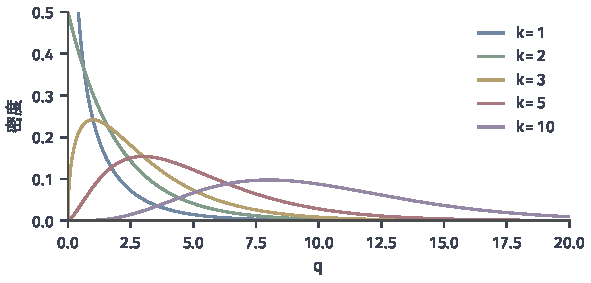
\includegraphics[width=100mm]{figures/01-basic-mathematics/05-probability-and-statistics-basics/matplotlib/samp-chi-square-densities/figure.pdf}
  \caption{自由度$k=1,2,3,5,10$的卡方分布密度，由式~\eqref{eq:samp-chi-square-density}计算。$\chi^2_k$的均值为$k$，方差为$2k$；自由度增大时分布右移、变宽，但相对其均值越来越集中且越来越对称。$k=1$时密度在$0$处趋于无穷，图中纵轴截断在$0.5$。}
  \label{fig:samp-chi-square-densities}
\end{figure}

\paragraph{样本方差的精确分布}
回到正态样本。定理~\ref{thm:samp-normal-mean-residual}的证明给出$(n-1)S_n^2=\lVert\bm R\rVert_2^2=\sigma^2\sum_{j=2}^nY_j^2$，其中$Y_2,\dots,Y_n$独立同分布于$\mathcal N(0,1)$。由定义~\ref{def:samp-chi-square}立即得到下面的结论。

\begin{theorem}[正态样本方差的分布]
\label{thm:samp-normal-sample-variance}
设$X_1,\dots,X_n$独立同分布于$\mathcal N(\mu,\sigma^2)$，$n\geq2$。则
\[
  \frac{(n-1)S_n^2}{\sigma^2}=\frac{1}{\sigma^2}\sum_{i=1}^n(X_i-\bar X_n)^2\sim\chi^2_{n-1},
\]
且它与$\bar X_n$相互独立。
\end{theorem}

自由度是$n-1$而不是$n$，原因在于残差落在$n-1$维子空间中。
如果$\mu$已知，$\sum_i(X_i-\mu)^2/\sigma^2=\sum_iZ_i^2$是$n$个独立标准正态的平方和，服从$\chi^2_n$；
改用样本均值作中心，相当于把$\bm Z$投影到与$\bm 1$正交的子空间，丢掉了沿$\bm 1$的那一个坐标$Y_1^2$。
这与第~\ref{sec:est-sample-variance}节中期望少了一个$\sigma^2$是同一现象的两种表现，只是这里得到的是完整的分布。

\begin{example}[样本方差的波动]
\label{ex:samp-sample-variance-distribution}
由定理~\ref{thm:samp-normal-sample-variance}和$\chi^2_{n-1}$的方差$2(n-1)$，
\[
  \operatorname{Var}S_n^2=\frac{\sigma^4}{(n-1)^2}\cdot2(n-1)=\frac{2\sigma^4}{n-1}.
\]
设$n=10$，$\sigma^2=4$。样本方差超过$6$的概率是$\mathbb{P}(\chi^2_9>9\cdot6/4)=\mathbb{P}(\chi^2_9>13.5)\approx0.141$：即使真实方差为$4$，也有约七分之一的机会得到大于$6$的样本方差。

这也让我们能比较两种方差估计的均方误差。$S_n^2$无偏，均方误差为$2\sigma^4/(n-1)$；
$\hat\sigma_n^2=\frac{n-1}nS_n^2$的方差为$\frac{2(n-1)\sigma^4}{n^2}$，偏差为$-\sigma^2/n$，按式~\eqref{eq:samp-mse-decomposition}，
\[
  \operatorname{MSE}(\hat\sigma_n^2)=\frac{2(n-1)\sigma^4}{n^2}+\frac{\sigma^4}{n^2}=\frac{(2n-1)\sigma^4}{n^2}.
\]
$n=10$时两者分别为$0.222\sigma^4$与$0.190\sigma^4$。在正态模型和均方误差标准下，有偏的$\hat\sigma_n^2$反而更好；这与示例~\ref{ex:samp-shrinkage}的收缩现象一致。
\end{example}

\subsection{Student $t$分布}
\label{sec:samp-t}

\paragraph{用随机标准差标准化}
若$\sigma$已知，$\sqrt n(\bar X_n-\mu)/\sigma\sim\mathcal N(0,1)$，可以直接查标准正态表。
$\sigma$未知时，自然的做法是用$S_n$代替$\sigma$，但分母因此也成了随机变量：$S_n$偶尔偏小时，比值会被放大。
我们需要一个分布描述“标准正态除以独立的随机标准差”。

\begin{definition}[$t$分布]
\label{def:samp-t}
设$Z\sim\mathcal N(0,1)$与$V\sim\chi^2_k$相互独立，称
\[
  T=\frac{Z}{\sqrt{V/k}}
\]
的分布为自由度为$k$的\term{$t$分布}（Student t distribution），记作$T\sim t_k$。
\end{definition}

分母中的$V/k$均值为$1$，是对“单位方差”的一个随机估计。
为求$T$的密度，写出$(Z,V)$的联合密度$\varphi(z)f_{\chi^2_k}(v)$，作变量替换$z=t\sqrt{v/k}$、$v=v$，Jacobian为$\sqrt{v/k}$（第~\ref{sec:rvec-transforms}节）。对$v$积分，并利用式~\eqref{eq:samp-chi-square-density}，
\[
  f_T(t)=\int_0^\infty\frac{1}{\sqrt{2\pi}}e^{-t^2v/(2k)}\sqrt{\frac vk}\cdot\frac{v^{k/2-1}e^{-v/2}}{2^{k/2}\Gamma(k/2)}\,\mathrm{d}v
  =\frac{1}{\sqrt{2\pi k}\,2^{k/2}\Gamma(k/2)}\int_0^\infty v^{\frac{k+1}2-1}e^{-\frac v2\left(1+\frac{t^2}k\right)}\,\mathrm{d}v.
\]
最后的积分是Gamma积分，等于$\Gamma\bigl(\frac{k+1}2\bigr)\bigl(\frac{2}{1+t^2/k}\bigr)^{(k+1)/2}$，化简后
\begin{equation}
  f_T(t)=\frac{\Gamma\bigl(\frac{k+1}2\bigr)}{\sqrt{k\pi}\,\Gamma\bigl(\frac k2\bigr)}\Bigl(1+\frac{t^2}{k}\Bigr)^{-(k+1)/2},\qquad t\in\mathbb{R}.
  \label{eq:samp-t-density}
\end{equation}

\paragraph{尾部与自由度}
式~\eqref{eq:samp-t-density}关于$t$对称，所以只要均值存在就等于$0$。
它的尾部按$|t|^{-(k+1)}$的幂次衰减，比正态密度的$e^{-t^2/2}$慢得多，这正是随机分母带来的额外波动。
自由度越小，尾部越重：$k=1$时$f_T(t)=\frac{1}{\pi(1+t^2)}$，即标准Cauchy分布，它的均值都不存在；一般地，$t_k$只有阶数小于$k$的矩，$k>2$时方差为$k/(k-2)$。
另一方面，$k\to\infty$时$(1+t^2/k)^{-(k+1)/2}\to e^{-t^2/2}$，$t_k$的密度逐点趋于标准正态密度，因为$V/k$越来越集中在$1$附近。

图~\ref{fig:samp-t-normal-tails}对照了几种$t$分布与标准正态。左图中$t$密度峰值更低、两侧更厚；右图用对数纵轴画双侧尾概率，差别在尾部被放大：
在$c=3$处，标准正态的尾概率约为$0.0027$，$t_{10}$约为$0.013$，$t_3$约为$0.058$，$t_1$约为$0.205$。

\begin{figure}[htbp]
  \centering
  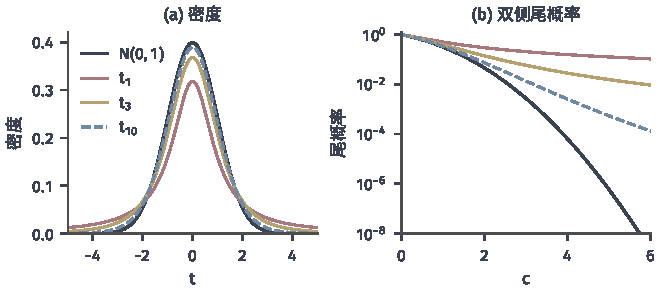
\includegraphics[width=112mm]{figures/01-basic-mathematics/05-probability-and-statistics-basics/matplotlib/samp-t-normal-tails/figure.pdf}
  \caption{Student $t$分布与标准正态分布的对照。(a) 自由度$k=1,3,10$的$t$密度与标准正态密度；(b) 双侧尾概率$\mathbb{P}(|T|>c)$，纵轴为对数刻度。自由度越小，峰越低、尾越重；$k$增大时曲线逐渐贴近标准正态。}
  \label{fig:samp-t-normal-tails}
\end{figure}

\paragraph{正态样本的$t$统计量}
定理~\ref{thm:samp-normal-mean-residual}与定理~\ref{thm:samp-normal-sample-variance}正好提供了定义~\ref{def:samp-t}所需的三个条件：
$Z=\sqrt n(\bar X_n-\mu)/\sigma\sim\mathcal N(0,1)$，$V=(n-1)S_n^2/\sigma^2\sim\chi^2_{n-1}$，且二者独立。代入定义，未知的$\sigma$恰好约去：
\begin{equation}
  T=\frac{\sqrt n(\bar X_n-\mu)}{S_n}=\frac{\sqrt n(\bar X_n-\mu)/\sigma}{\sqrt{\frac{(n-1)S_n^2/\sigma^2}{n-1}}}\sim t_{n-1}.
  \label{eq:samp-t-statistic}
\end{equation}
统计量$T$只含样本和待研究的$\mu$，它的分布不依赖任何未知参数；第~\ref{chap:intervals-tests-prediction}章将用这一点构造均值的区间与检验。

\begin{example}[用样本标准差标准化的代价]
\label{ex:samp-t-quantiles}
设$n=10$。若误把$T$当作标准正态，以为$\mathbb{P}(|T|>1.96)=0.05$，实际概率是$\mathbb{P}(|t_9|>1.96)\approx0.082$，几乎多出三分之二。
要使双侧尾概率真正为$0.05$，需要$t_{9,0.975}\approx2.262$。
下表列出不同样本量下$t_{n-1,0.975}$与$z_{0.975}\approx1.96$的比较：样本越小，用样本标准差代替$\sigma$的代价越大。
\begin{center}
\begin{tabular}{lccccc}
\toprule
$n$ & $5$ & $10$ & $30$ & $100$ & $\infty$ \\
\midrule
$t_{n-1,0.975}$ & $2.776$ & $2.262$ & $2.045$ & $1.984$ & $1.960$ \\
\bottomrule
\end{tabular}
\end{center}
\end{example}

\subsection{$F$分布}
\label{sec:samp-f}

\paragraph{两个卡方变量之比}
比较两组数据的波动时，自然的统计量是两个样本方差之比。
每个样本方差（适当缩放后）都是卡方变量，各除以自己的自由度后变成“平均每个自由度的平方长度”，再取比值。

\begin{definition}[$F$分布]
\label{def:samp-f}
设$V_1\sim\chi^2_{k_1}$与$V_2\sim\chi^2_{k_2}$相互独立，称
\[
  F=\frac{V_1/k_1}{V_2/k_2}
\]
的分布为自由度为$(k_1,k_2)$的\term{$F$分布}（F distribution），记作$F\sim F_{k_1,k_2}$。$k_1$称为分子自由度，$k_2$称为分母自由度。
\end{definition}

两个自由度分别来自分子与分母中的卡方变量，交换分子分母就交换它们：$1/F\sim F_{k_2,k_1}$。
若$T\sim t_k$，则$T^2=Z^2/(V/k)$，分子$Z^2\sim\chi^2_1$，所以$T^2\sim F_{1,k}$，$t$分布与$F$分布由此相连。
仿照$t$密度的推导，对$(V_1,V_2)$作变量替换并对辅助变量积分，可以得到$r>0$处的密度
\[
  f_{F_{k_1,k_2}}(r)=\frac{1}{B\bigl(\frac{k_1}2,\frac{k_2}2\bigr)}\Bigl(\frac{k_1}{k_2}\Bigr)^{k_1/2}r^{k_1/2-1}\Bigl(1+\frac{k_1}{k_2}r\Bigr)^{-(k_1+k_2)/2},
\]
其中$B(a,b)=\int_0^1u^{a-1}(1-u)^{b-1}\,\mathrm{d}u$是第~\ref{sec:prob-beta}节的Beta积分。

\paragraph{均值与形状}
由独立性，$\mathbb{E}F=\mathbb{E}\frac{V_1}{k_1}\cdot k_2\mathbb{E}\frac1{V_2}$。第一个因子为$1$；当$k_2>2$时，利用式~\eqref{eq:samp-chi-square-density}，
\[
  \mathbb{E}\frac1{V_2}=\int_0^\infty\frac{q^{k_2/2-2}e^{-q/2}}{2^{k_2/2}\Gamma(k_2/2)}\,\mathrm{d}q=\frac{2^{k_2/2-1}\Gamma(k_2/2-1)}{2^{k_2/2}\Gamma(k_2/2)}=\frac{1}{k_2-2},
\]
所以$\mathbb{E}F=k_2/(k_2-2)$，略大于$1$。
图~\ref{fig:samp-f-densities}显示，两个自由度都较小时$F$分布右偏、尾部很长；自由度都增大时，两个“平均平方长度”都集中在$1$附近，比值也集中在$1$附近。

\begin{figure}[htbp]
  \centering
  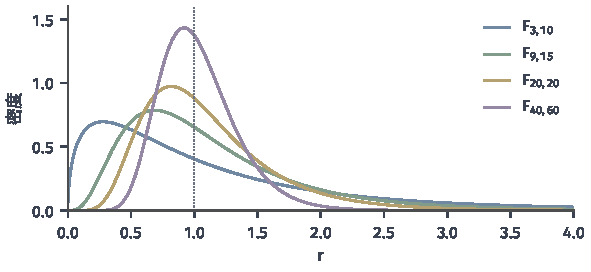
\includegraphics[width=100mm]{figures/01-basic-mathematics/05-probability-and-statistics-basics/matplotlib/samp-f-densities/figure.pdf}
  \caption{几组自由度$(k_1,k_2)$下的$F$分布密度。点线标出$r=1$。自由度小时分布右偏、尾长；两个自由度都增大时，分布向$1$附近收拢。}
  \label{fig:samp-f-densities}
\end{figure}

\paragraph{两个正态样本的方差比}
设$X_1,\dots,X_{n_1}$独立同分布于$\mathcal N(\mu_1,\sigma_1^2)$，$Y_1,\dots,Y_{n_2}$独立同分布于$\mathcal N(\mu_2,\sigma_2^2)$，两组样本相互独立，样本方差分别为$S_1^2$与$S_2^2$。
由定理~\ref{thm:samp-normal-sample-variance}，$(n_1-1)S_1^2/\sigma_1^2\sim\chi^2_{n_1-1}$，$(n_2-1)S_2^2/\sigma_2^2\sim\chi^2_{n_2-1}$，二者分别是两组独立样本的函数，因而独立。代入定义~\ref{def:samp-f}，
\begin{equation}
  \frac{S_1^2/\sigma_1^2}{S_2^2/\sigma_2^2}\sim F_{n_1-1,\,n_2-1}.
  \label{eq:samp-variance-ratio}
\end{equation}
当$\sigma_1^2=\sigma_2^2$时，未知方差约去，$S_1^2/S_2^2$本身就服从$F_{n_1-1,n_2-1}$。

\begin{example}[方差比的波动范围]
\label{ex:samp-variance-ratio}
设$n_1=10$，$n_2=16$，两总体方差相等。即使如此，$S_1^2/S_2^2\geq2.5$的概率仍为$\mathbb{P}(F_{9,15}\geq2.5)\approx0.056$；
上侧$5\%$的分界点是$F_{9,15,0.95}\approx2.59$。
所以在这样的小样本中，一个样本方差是另一个的两倍多并不罕见；第~\ref{chap:intervals-tests-prediction}章的方差比较正是以式~\eqref{eq:samp-variance-ratio}作为精确依据。
需要注意，这一结论依赖两个总体都是正态的；总体尾部较重时，样本方差的波动更大，$F$分布会低估方差比的极端程度。
\end{example}

\section{有限样本的概率界}
\label{sec:samp-bounds}
\label{sec:rv-features}

上一节的精确分布依赖正态假设。很多时候我们只知道总体的均值或方差，甚至只知道观测有界，却仍然希望对一个确定的样本量说出“误差超过某个值的概率不超过多少”。
本节的两个不等式只用矩信息就能给出这种保证。它们不要求样本量足够大，代价是给出的往往只是较宽松的上界。

\subsection{Markov不等式}

\paragraph{从期望控制尾概率}
如果一个非负随机变量经常取很大的值，它的期望就不可能很小。把这一直觉定量化，就得到用期望控制尾概率的\term{Markov不等式}（Markov inequality）。

\begin{theorem}[Markov不等式]
\label{thm:samp-markov}
设$X\geq0$，$\mathbb{E}X$有限，$a>0$。则
\begin{equation}
  \mathbb{P}(X\geq a)\leq\frac{\mathbb{E}X}{a}.
  \label{eq:samp-markov-inequality}
\end{equation}
\end{theorem}

\begin{proof}
考虑事件$\{X\geq a\}$的指示变量$\mathbb{I}_{\{X\geq a\}}$。在该事件上$X\geq a=a\,\mathbb{I}_{\{X\geq a\}}$；在其补事件上$X\geq0=a\,\mathbb{I}_{\{X\geq a\}}$。所以总有$X\geq a\,\mathbb{I}_{\{X\geq a\}}$，两边取期望，
\[
  \mathbb{E}X\geq a\,\mathbb{E}\,\mathbb{I}_{\{X\geq a\}}=a\,\mathbb{P}(X\geq a).
\]
两边除以$a>0$即得结论。
\end{proof}

证明只丢掉了两部分：事件$\{X<a\}$上$X$对期望的贡献，以及事件$\{X\geq a\}$上$X$超出$a$的部分。
两部分都为零时等号成立：例如$X$只取$0$与$a$两个值，$\mathbb{P}(X=a)=\mathbb{E}X/a$。所以只知道均值时，式~\eqref{eq:samp-markov-inequality}不能再改进。

\paragraph{条件的作用}
非负性不能去掉。若$X$以各$1/2$的概率取$-10$与$10$，则$\mathbb{E}X=0$，右端为$0$，而$\mathbb{P}(X\geq10)=1/2$：负值部分把期望拉低，抵消了大取值的贡献。
阈值必须为正，否则除法无意义；当$a\leq\mathbb{E}X$时右端不小于$1$，不等式虽然成立却没有提供信息。
对于可能取负值的变量，常见做法是先作非负变换，例如考虑$|X|$或$(X-\mu)^2$，这正是下一小节的思路。

\begin{example}[指数分布的尾概率]
\label{ex:samp-markov-exponential}
设$X$服从率参数为$1$的指数分布，$\mathbb{E}X=1$。Markov不等式给出$\mathbb{P}(X\geq3)\leq1/3$，而真实值是$e^{-3}\approx0.050$，上界大了六倍多。
图~\ref{fig:samp-markov-chebyshev}(a)显示，阈值越大差距越大：上界按$1/a$缓慢下降，真实尾概率按$e^{-a}$指数下降。
Markov不等式只利用了均值，它必须对所有均值为$1$的非负分布同时成立，其中包括上面那种把质量集中在$0$与$a$两点的极端分布，所以对具体的指数分布显得保守。
\end{example}

\begin{figure}[htbp]
  \centering
  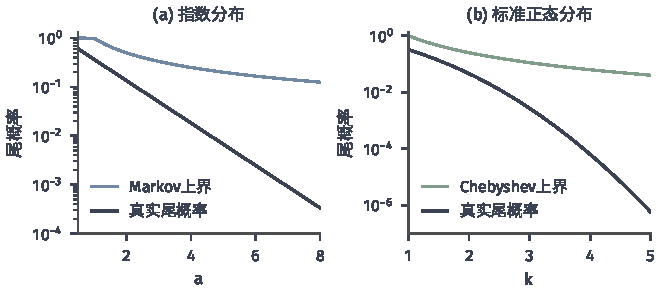
\includegraphics[width=112mm]{figures/01-basic-mathematics/05-probability-and-statistics-basics/matplotlib/samp-markov-chebyshev/figure.pdf}
  \caption{矩不等式给出的上界与真实尾概率，纵轴为对数刻度。(a) $X$服从率参数为$1$的指数分布：Markov上界$\min(1,1/a)$与真实值$\mathbb{P}(X\geq a)=e^{-a}$；(b) $Z\sim\mathcal N(0,1)$：Chebyshev上界$1/k^2$与真实值$\mathbb{P}(|Z|\geq k)$。两个上界都随阈值多项式下降，真实尾概率下降得快得多。}
  \label{fig:samp-markov-chebyshev}
\end{figure}

\subsection{Chebyshev不等式}

\paragraph{作用于平方偏离}
对一般随机变量，我们关心的是它偏离均值的程度。偏离$X-\mu$可正可负，平方解决了这个问题：$(X-\mu)^2$非负，期望恰为方差。对它使用Markov不等式，就得到\term{Chebyshev不等式}（Chebyshev inequality）。

\begin{theorem}[Chebyshev不等式]
\label{thm:samp-chebyshev}
设$X$的均值为$\mu$，方差$\sigma^2$有限。则对任意$t>0$，
\begin{equation}
  \mathbb{P}(|X-\mu|\geq t)\leq\frac{\sigma^2}{t^2}.
  \label{eq:probability-chebyshev-inequality}
\end{equation}
\end{theorem}

\begin{proof}
事件$\{|X-\mu|\geq t\}$与$\{(X-\mu)^2\geq t^2\}$相同。对非负变量$(X-\mu)^2$与阈值$t^2>0$应用Markov不等式，
\[
  \mathbb{P}(|X-\mu|\geq t)=\mathbb{P}\bigl((X-\mu)^2\geq t^2\bigr)\leq\frac{\mathbb{E}(X-\mu)^2}{t^2}=\frac{\sigma^2}{t^2}.
\]
\end{proof}

当$\sigma>0$时取$t=k\sigma$，得到更便于记忆的形式$\mathbb{P}(|X-\mu|\geq k\sigma)\leq1/k^2$：任何有限方差的分布，偏离均值两个标准差以上的概率不超过$1/4$，三个标准差以上不超过$1/9$。
和Markov不等式一样，这个界在只知道均值和方差时不能再改进：取$X$以概率$\frac1{2k^2}$分别等于$\mu\pm k\sigma$、以概率$1-\frac1{k^2}$等于$\mu$（$k\geq1$），它的方差恰为$\sigma^2$，并使等号成立。

\paragraph{与正态精确概率的对照}

\begin{example}[两个标准差与三个标准差]
\label{ex:samp-chebyshev-normal}
若$X\sim\mathcal N(\mu,\sigma^2)$，标准化后$\mathbb{P}(|X-\mu|\geq2\sigma)=2(1-\Phi(2))\approx0.046$，$\mathbb{P}(|X-\mu|\geq3\sigma)\approx0.0027$。
Chebyshev不等式给出的对应上界是$0.25$与$0.111$，分别大了约$5$倍与$40$倍。
\end{example}

这一对照说明了两类依据的区别。
正态模型给出精确概率，但只在正态假设成立时才对；Chebyshev上界对一切有限方差的分布都成立，所以必须照顾到最极端的分布，对于正态这样尾部很轻的分布就显得宽松。
图~\ref{fig:samp-markov-chebyshev}(b)把差距画在对数刻度上：上界按$1/k^2$下降，正态尾概率按$e^{-k^2/2}$量级下降。
减少分布假设与获得较紧的结论不可兼得，选择哪一种取决于我们对总体有多少可靠信息。

\subsection{样本均值误差与样本量}

\paragraph{误差、失败概率与样本量}
把Chebyshev不等式用于样本均值。设$X_1,\dots,X_n$独立同分布，均值$\mu$，方差$\sigma^2$有限。由式~\eqref{eq:samp-mean-standard-error}，$\operatorname{Var}\bar X_n=\sigma^2/n$，于是对任意$\varepsilon>0$，
\begin{equation}
  \mathbb{P}\bigl(|\bar X_n-\mu|\geq\varepsilon\bigr)\leq\frac{\sigma^2}{n\varepsilon^2}.
  \label{eq:samp-mean-chebyshev}
\end{equation}
式中出现三个量：允许的误差$\varepsilon$、误差超过$\varepsilon$的“失败概率”，以及样本量$n$。
若要求失败概率不超过$\delta\in(0,1)$，只需$\sigma^2/(n\varepsilon^2)\leq\delta$，即
\[
  n\geq\frac{\sigma^2}{\delta\varepsilon^2}.
\]
误差减半，所需样本量变为四倍；失败概率减为十分之一，所需样本量变为十倍。
例如仪器单次读数的标准差已知为$\sigma=2$，要求平均读数的误差小于$0.5$的概率至少为$0.9$，即$\varepsilon=0.5$、$\delta=0.1$，则$n\geq4/(0.1\times0.25)=160$次重复测量足以保证，且不需要知道读数服从什么分布。

\paragraph{Bernoulli均值的样本量设计}
对比例$p$，$\sigma^2=p(1-p)$依赖未知的$p$。但$p(1-p)=\frac14-(p-\frac12)^2\leq\frac14$，用这个上界代替$\sigma^2$，得到对所有$p$都有效的设计。

\begin{example}[估计支持率需要多少样本]
\label{ex:samp-chebyshev-sample-size}
希望样本比例与真实比例之差小于$0.05$的概率至少为$0.95$，即$\varepsilon=0.05$，$\delta=0.05$。由$p(1-p)\leq1/4$，
\[
  n\geq\frac{1/4}{0.05\cdot0.05^2}=2000
\]
就足够，无论$p$是多少。
这个数字偏保守。$p=1/2$时可以用二项分布直接计算失败概率：图~\ref{fig:samp-chebyshev-sample-size}显示，从$n=401$起精确失败概率就都不超过$0.05$了，只有Chebyshev要求的五分之一左右。
差距的来源与示例~\ref{ex:samp-chebyshev-normal}相同：式~\eqref{eq:samp-mean-chebyshev}只用了方差。
\end{example}

\begin{figure}[htbp]
  \centering
  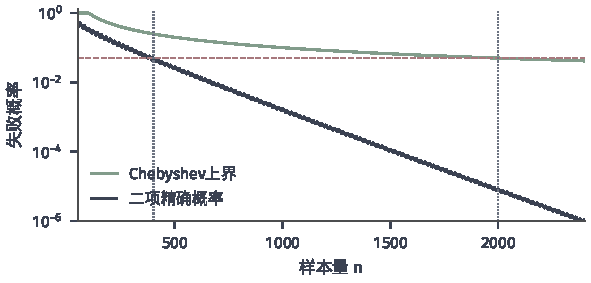
\includegraphics[width=100mm]{figures/01-basic-mathematics/05-probability-and-statistics-basics/matplotlib/samp-chebyshev-sample-size/figure.pdf}
  \caption{样本比例的失败概率$\mathbb{P}(|\hat p-0.5|\geq0.05)$随样本量$n$的变化，总体为$\operatorname{Bernoulli}(0.5)$，纵轴为对数刻度。Chebyshev上界为$100/n$，在$n=2000$处降到$0.05$（虚线）；二项分布精确概率从$n=401$起不超过$0.05$。精确曲线的锯齿来自样本比例只能取离散值。}
  \label{fig:samp-chebyshev-sample-size}
\end{figure}

\paragraph{不能直接代入样本方差}
若总体方差未知，人们容易想到先抽样算出$S_n^2$，再把它代入$\sigma^2/(n\varepsilon^2)$。
这样做得到的数是随机的，式~\eqref{eq:samp-mean-chebyshev}的证明却要求右端是确定的$\sigma^2$：
当这次样本恰好低估了方差时，计算出的“上界”偏小，而这类样本出现的概率并没有被控制，原来的严格保证因此不再成立。
要保留严格保证，需要一个预先可靠的方差上界（如比例问题中的$1/4$，或观测有界时由取值范围给出的上界）；
否则只能借助正态模型下的$t$分布或大样本下的近似，第~\ref{sec:samp-clt}节将说明后者的依据。

\section{大数定律与估计的一致性}
\label{sec:samp-lln}

式~\eqref{eq:samp-mean-chebyshev}的右端随$n\to\infty$趋于零，说明样本量增大时，样本均值偏离总体均值的概率越来越小。
本节先给这种“随机误差趋于零”的方式命名，再证明弱大数定律，最后把它用于估计量，得到一致性。

\subsection{依概率收敛}

\paragraph{定义}
对随机变量序列，“误差趋于零”可以有多种含义。我们这里采用最直接的一种：对任意固定的容许误差，误差超过它的概率趋于零。

\begin{definition}[依概率收敛]
\label{def:samp-convergence-in-probability}
设$Y_1,Y_2,\dots$与$Y$是同一随机试验中的随机变量。若对任意$\varepsilon>0$，
\[
  \lim_{n\to\infty}\mathbb{P}\bigl(|Y_n-Y|\geq\varepsilon\bigr)=0,
\]
称$Y_n$\term{依概率收敛}（convergence in probability）于$Y$，记作$Y_n\xrightarrow{\mathbb{P}}Y$。
\end{definition}

本章用到的极限$Y$几乎都是常数$c$，此时定义只涉及每个$Y_n$自己的分布：$\mathbb{P}(|Y_n-c|\geq\varepsilon)\to0$。
这里的极限是第~\ref{sec:ru-sequence-limits}节意义下的数列极限，对象是数列$a_n=\mathbb{P}(|Y_n-c|\geq\varepsilon)$；$\varepsilon$越小，通常需要越大的$n$才能使$a_n$变小。
由式~\eqref{eq:samp-mean-chebyshev}，在有限方差下$\bar X_n\xrightarrow{\mathbb{P}}\mu$，这就是下一小节的第一个定理。

\paragraph{它不保证什么}
依概率收敛描述的是每个固定$n$下误差分布的集中程度，它不要求误差随$n$单调减小。
图~\ref{fig:samp-running-means}(a)中的每一条路径都是同一组观测逐个累加时样本均值的变化：路径在前几十步内大幅上下摆动，偶尔还会离开阴影带；
但对每个固定的大$n$，绝大多数路径都已落在带内。

依概率收敛也不等于“沿着每一条观测序列，数值序列都收敛”。下面这个例子中，每个固定$n$处出错的概率都趋于零，但没有任何一条路径收敛。

\begin{example}[出错概率趋于零而路径不收敛]
\label{ex:samp-typewriter}
设$U\sim\operatorname{U}(0,1)$。把区间$[0,1)$依次分成$1$段、$2$段、$3$段……，每一轮把各段从左到右排成序列：
$[0,1)$，$[0,\tfrac12)$，$[\tfrac12,1)$，$[0,\tfrac13)$，$[\tfrac13,\tfrac23)$，$[\tfrac23,1)$，……，第$n$段记作$I_n$，令$Y_n=\mathbb{I}_{\{U\in I_n\}}$。
若$I_n$属于分成$k$段的那一轮，则$\mathbb{P}(Y_n\ne0)=1/k$，而$k\to\infty$，所以$Y_n\xrightarrow{\mathbb{P}}0$。
但对任意取定的$u\in[0,1)$，每一轮恰有一段包含$u$，所以数列$Y_n(u)$中有无穷多个$1$，也有无穷多个$0$，并不收敛。
\end{example}

沿路径的收敛是更强的要求，它属于随机变量收敛的一般理论，留到\BookPartRef{part:probability-spaces}{卷2《数学准备：抽象数学》的“概率空间”部分}。本部分只需要依概率收敛。

\subsection{弱大数定律}

\paragraph{有限方差的情形}

\begin{theorem}[弱大数定律：有限方差]
\label{thm:samp-wlln-variance}
设$X_1,X_2,\dots$独立同分布，均值$\mu$，方差$\sigma^2$有限。则$\bar X_n\xrightarrow{\mathbb{P}}\mu$。
\end{theorem}

\begin{proof}
对任意$\varepsilon>0$，由式~\eqref{eq:samp-mean-chebyshev}，$0\leq\mathbb{P}(|\bar X_n-\mu|\geq\varepsilon)\leq\sigma^2/(n\varepsilon^2)$，右端随$n\to\infty$趋于零。
\end{proof}

这个定理通常称为\term{弱大数定律}（weak law of large numbers）。“弱”指结论是依概率收敛，而不是沿路径的收敛。
它最早的形式针对事件频率。

\begin{example}[频率趋于概率]
\label{ex:samp-frequency-lln}
重复做独立试验，事件$A$每次发生的概率为$p$。令$X_i=\mathbb{I}_{\{\text{第}i\text{次试验中}A\text{发生}\}}$，则$X_i\sim\operatorname{Bernoulli}(p)$，$\bar X_n$就是前$n$次试验中$A$发生的频率。
由定理~\ref{thm:samp-wlln-variance}，频率依概率收敛于$p$；并且$\mathbb{P}(|\bar X_n-p|\geq\varepsilon)\leq p(1-p)/(n\varepsilon^2)\leq1/(4n\varepsilon^2)$。
图~\ref{fig:samp-running-means}(a)取$p=0.3$画出了六条频率路径，到$n=5000$时它们都落在$0.30\pm0.013$之内。
\end{example}

\begin{figure}[htbp]
  \centering
  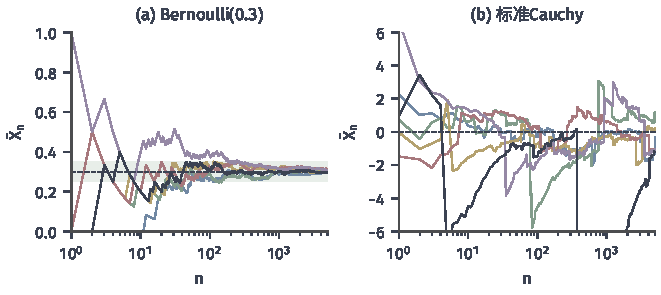
\includegraphics[width=112mm]{figures/01-basic-mathematics/05-probability-and-statistics-basics/matplotlib/samp-running-means/figure.pdf}
  \caption{样本均值$\bar X_n$随样本量$n$的变化，横轴为对数刻度，每个面板用固定随机种子画出六条独立路径。(a) 总体为$\operatorname{Bernoulli}(0.3)$，阴影带为$0.3\pm0.05$，各路径逐渐进入并停留在带内；(b) 总体为标准Cauchy分布，它没有均值，路径不断出现大跳跃，没有稳定下来的趋势（纵轴截断在$\pm6$）。}
  \label{fig:samp-running-means}
\end{figure}

\paragraph{只有一阶绝对矩的情形}
定理~\ref{thm:samp-wlln-variance}要求方差有限。但结论本身只涉及均值，我们希望在只假设$\mathbb{E}|X|<\infty$时也能得到它。
这不只是为了推广而推广：第~\ref{sec:samp-consistency}节要对$X_i^2$使用大数定律来研究样本方差，若仍要求$X_i^2$的方差有限，就需要$\mathbb{E}X^4<\infty$，比我们想要的“$X$方差有限”强得多。
另一方面，也不能完全不要矩条件：图~\ref{fig:samp-running-means}(b)中的标准Cauchy分布没有均值，可以证明它的样本均值对每个$n$都仍服从标准Cauchy分布，不会集中到任何数附近；证明需要特征函数等工具，本部分不展开。

没有方差时，Chebyshev不等式不能直接使用。思路是把每个观测分成两部分：绝对值不超过$M$的有界部分有方差，可以用Chebyshev；超过$M$的尾部方差可能不存在，但它的一阶绝对矩可以通过选大$M$变得很小，再用Markov控制。

\begin{theorem}[弱大数定律：有限一阶绝对矩]
\label{thm:samp-wlln-first-moment}
设$X_1,X_2,\dots$独立同分布，$\mathbb{E}|X_1|<\infty$，$\mu=\mathbb{E}X_1$。则$\bar X_n\xrightarrow{\mathbb{P}}\mu$。
\end{theorem}

\begin{proof}
固定$\varepsilon>0$与$\eta>0$。我们要找到$N$，使$n\geq N$时$\mathbb{P}(|\bar X_n-\mu|\geq\varepsilon)<\eta$。

\emph{第一步：截断。}对常数$M>0$，令
\[
  Y_i=X_i\,\mathbb{I}_{\{|X_i|\leq M\}},\qquad W_i=X_i\,\mathbb{I}_{\{|X_i|>M\}},
\]
则$X_i=Y_i+W_i$。$Y_1,Y_2,\dots$是各自$X_i$的函数，因而独立同分布，且$|Y_i|\leq M$；$W_i$同理。
记$\mu_M=\mathbb{E}Y_1$，$\nu_M=\mathbb{E}W_1$，则$\mu=\mu_M+\nu_M$，于是
\[
  \bar X_n-\mu=(\bar Y_n-\mu_M)+(\bar W_n-\nu_M).
\]
若$|\bar X_n-\mu|\geq\varepsilon$，两项中至少有一项的绝对值不小于$\varepsilon/2$，所以
\begin{equation}
  \mathbb{P}(|\bar X_n-\mu|\geq\varepsilon)\leq\mathbb{P}\Bigl(|\bar Y_n-\mu_M|\geq\frac\varepsilon2\Bigr)+\mathbb{P}\Bigl(|\bar W_n-\nu_M|\geq\frac\varepsilon2\Bigr).
  \label{eq:samp-truncation-split}
\end{equation}

\emph{第二步：用Markov控制尾部。}记$t_M=\mathbb{E}|W_1|=\mathbb{E}\bigl[|X_1|\,\mathbb{I}_{\{|X_1|>M\}}\bigr]$。由三角不等式与期望的线性性，
\[
  \mathbb{E}|\bar W_n-\nu_M|\leq\frac1n\sum_{i=1}^n\mathbb{E}|W_i|+|\nu_M|\leq t_M+t_M=2t_M,
\]
其中$|\nu_M|=|\mathbb{E}W_1|\leq\mathbb{E}|W_1|$。对非负变量$|\bar W_n-\nu_M|$用Markov不等式，
\[
  \mathbb{P}\Bigl(|\bar W_n-\nu_M|\geq\frac\varepsilon2\Bigr)\leq\frac{2t_M}{\varepsilon/2}=\frac{4t_M}{\varepsilon}.
\]
这个界与$n$无关。它能变小，是因为$t_M\to0$（$M\to\infty$）：在离散情形，$t_M=\sum_{|x|>M}|x|\,p_{X}(x)$是收敛级数$\sum_x|x|\,p_X(x)=\mathbb{E}|X_1|$的尾部；在有密度的情形，$t_M=\int_{|x|>M}|x|f_X(x)\,\mathrm{d}x$是收敛反常积分的尾部；两者都随$M\to\infty$趋于零。
于是可以先取定$M$，使$4t_M/\varepsilon<\eta/2$。

\emph{第三步：用Chebyshev控制有界部分。}$M$取定后，$\operatorname{Var}Y_1\leq\mathbb{E}Y_1^2\leq M^2$。由式~\eqref{eq:samp-mean-chebyshev}，
\[
  \mathbb{P}\Bigl(|\bar Y_n-\mu_M|\geq\frac\varepsilon2\Bigr)\leq\frac{M^2}{n(\varepsilon/2)^2}=\frac{4M^2}{n\varepsilon^2}.
\]
再取$N$使$4M^2/(N\varepsilon^2)<\eta/2$。代入式~\eqref{eq:samp-truncation-split}，当$n\geq N$时$\mathbb{P}(|\bar X_n-\mu|\geq\varepsilon)<\eta/2+\eta/2=\eta$。由$\eta$的任意性，结论成立。
\end{proof}

证明中两个参数的选取顺序不能颠倒。$M$越大，尾部的贡献$4t_M/\varepsilon$越小，但有界部分的上界$4M^2/(n\varepsilon^2)$越大；
若先固定$n$再选$M$，两者无法同时变小。先用$M$把尾部压到$\eta/2$以下，这一步与$n$无关；再让$n$增大去抵消已经固定的$M^2$。
截断把“没有方差”的问题化成了“有方差但方差很大”的问题，而样本量正好可以对付后者。

\subsection{估计量的一致性}
\label{sec:samp-consistency}

\paragraph{定义及与无偏性的比较}
大数定律说的是样本均值，我们把同样的要求放到一般估计量上：样本越来越多时，估计误差超过任何固定容许值的概率都趋于零。

\begin{definition}[一致性]
\label{def:samp-consistency}
设对每个样本量$n$，$\hat\theta_n$是用$X_1,\dots,X_n$构造的$\theta$的估计量。若对每个$\theta\in\Theta$，当样本按参数$\theta$生成时都有$\hat\theta_n\xrightarrow{\mathbb{P}}\theta$，称估计量序列$\{\hat\theta_n\}$具有\term{一致性}（consistency），也称它是$\theta$的一致估计量。
\end{definition}

一致性与无偏性回答的是不同的问题。无偏性固定样本量，问抽样分布的中心是否对准目标；一致性让样本量增大，问抽样分布最终是否集中到目标上。两者互不蕴含：
\begin{itemize}
  \item 只用第一个观测的$\hat\mu_n=X_1$对每个$n$都无偏，但它的分布不随$n$改变，只要$\sigma>0$就不一致。
  \item $\hat\sigma_n^2$对每个$n$都有偏，偏差$-\sigma^2/n$随$n$消失；下面会证明它是一致的。
\end{itemize}
两者之间有一个常用的联系：若$\operatorname{MSE}_\theta(\hat\theta_n)\to0$，则对$(\hat\theta_n-\theta)^2$用Markov不等式，
\[
  \mathbb{P}\bigl(|\hat\theta_n-\theta|\geq\varepsilon\bigr)\leq\frac{\operatorname{MSE}_\theta(\hat\theta_n)}{\varepsilon^2}\to0.
\]
结合式~\eqref{eq:samp-mse-decomposition}，方差与偏差都趋于零的估计量是一致的。示例~\ref{ex:samp-uniform-mse}中的三个估计量都满足这一条件。

\paragraph{依概率收敛的运算}
许多估计量是若干样本平均的连续函数。下面的引理说明，依概率收敛到常数的性质在连续函数下保持。

\begin{lemma}[连续函数保持依概率收敛]
\label{lem:samp-continuous-mapping}
设$U_n\xrightarrow{\mathbb{P}}a$，$V_n\xrightarrow{\mathbb{P}}b$，$a,b$为常数，二元函数$g$在点$(a,b)$连续。则$g(U_n,V_n)\xrightarrow{\mathbb{P}}g(a,b)$。
特别地，$U_n+V_n\xrightarrow{\mathbb{P}}a+b$，$U_nV_n\xrightarrow{\mathbb{P}}ab$；$b\neq0$时$U_n/V_n\xrightarrow{\mathbb{P}}a/b$。一元函数是其特例。
\end{lemma}

\begin{proof}
给定$\varepsilon>0$。由$g$在$(a,b)$连续，存在$\delta>0$，使$|u-a|<\delta$且$|v-b|<\delta$时$|g(u,v)-g(a,b)|<\varepsilon$。
因此事件$\{|g(U_n,V_n)-g(a,b)|\geq\varepsilon\}$包含于$\{|U_n-a|\geq\delta\}\cup\{|V_n-b|\geq\delta\}$，
\[
  \mathbb{P}\bigl(|g(U_n,V_n)-g(a,b)|\geq\varepsilon\bigr)\leq\mathbb{P}(|U_n-a|\geq\delta)+\mathbb{P}(|V_n-b|\geq\delta)\to0.
\]
比值情形中$g(u,v)=u/v$在$v=b\neq0$处连续；$V_n=0$的事件包含于$\{|V_n-b|\geq|b|\}$，其概率趋于零，不影响结论。
\end{proof}

\paragraph{样本矩与样本方差}
现在可以处理第~\ref{chap:sample-estimation}章的常用估计量。

\begin{theorem}[样本矩与样本方差的一致性]
\label{thm:samp-moment-consistency}
设$X_1,X_2,\dots$独立同分布。
\begin{enumerate}
  \item 若$\mathbb{E}|X_1|^k<\infty$，则第$k$阶样本原点矩$\frac1n\sum_{i=1}^nX_i^k\xrightarrow{\mathbb{P}}\mathbb{E}X_1^k$。
  \item 若$\mathbb{E}X_1^2<\infty$，记$\sigma^2=\operatorname{Var}X_1$，则$\hat\sigma_n^2\xrightarrow{\mathbb{P}}\sigma^2$，$S_n^2\xrightarrow{\mathbb{P}}\sigma^2$。
\end{enumerate}
\end{theorem}

\begin{proof}
(1) $X_1^k,X_2^k,\dots$独立同分布，且一阶绝对矩$\mathbb{E}|X_1^k|$有限，由定理~\ref{thm:samp-wlln-first-moment}即得。

(2) 展开平方，
\[
  \hat\sigma_n^2=\frac1n\sum_{i=1}^n(X_i-\bar X_n)^2=\frac1n\sum_{i=1}^nX_i^2-\bar X_n^2.
\]
由(1)取$k=2$与$k=1$，$\frac1n\sum_iX_i^2\xrightarrow{\mathbb{P}}\mathbb{E}X_1^2$，$\bar X_n\xrightarrow{\mathbb{P}}\mu$。对$g(u,v)=u-v^2$用引理~\ref{lem:samp-continuous-mapping}，$\hat\sigma_n^2\xrightarrow{\mathbb{P}}\mathbb{E}X_1^2-\mu^2=\sigma^2$。
最后$S_n^2=\frac{n}{n-1}\hat\sigma_n^2$，而确定的数列$\frac n{n-1}\to1$，再用一次引理即得。
\end{proof}

这里正是第~\ref{sec:samp-lln}节保留截断论证的原因：对$X_i^2$使用大数定律时，我们只知道$\mathbb{E}|X_i^2|=\mathbb{E}X_1^2<\infty$，不知道$X_i^2$的方差是否有限。

\begin{example}[矩估计的一致性]
\label{ex:samp-exponential-rate-consistency}
设$X_1,X_2,\dots$独立同分布于率参数为$\lambda$的指数分布。第~\ref{sec:est-moments}节的矩估计（也是第~\ref{sec:est-mle}节的最大似然估计）为$\hat\lambda_n=1/\bar X_n$。
由大数定律，$\bar X_n\xrightarrow{\mathbb{P}}1/\lambda>0$；函数$g(v)=1/v$在$1/\lambda$处连续，由引理~\ref{lem:samp-continuous-mapping}，$\hat\lambda_n\xrightarrow{\mathbb{P}}\lambda$。
注意$\hat\lambda_n$并不无偏：可以算出$n\geq2$时$\mathbb{E}\hat\lambda_n=\frac{n}{n-1}\lambda$。一致性不需要先算出期望。
\end{example}

\paragraph{固定阈值处的经验分布函数}
第~\ref{sec:est-empirical-cdf}节的经验分布函数在每个固定点$x$处是一个Bernoulli平均：
\[
  \hat F_n(x)=\frac1n\sum_{i=1}^n\mathbb{I}_{\{X_i\leq x\}},\qquad \mathbb{I}_{\{X_i\leq x\}}\sim\operatorname{Bernoulli}\bigl(F(x)\bigr).
\]
所以$\mathbb{E}\hat F_n(x)=F(x)$，$\operatorname{Var}\hat F_n(x)=F(x)(1-F(x))/n\leq1/(4n)$，由弱大数定律$\hat F_n(x)\xrightarrow{\mathbb{P}}F(x)$。
图~\ref{fig:samp-three-distributions}(b)中的阶梯在每个固定位置与总体曲线的差距，随样本量增大而缩小，就是这一结论。
这里的结论对每个$x$分别成立；“整条经验分布函数一致地靠近$F$”需要同时控制无穷多个点，属于更深的结果，本部分不展开。

\section{中心极限定理与正态近似}
\label{sec:samp-clt}

大数定律告诉我们$\bar X_n-\mu$依概率趋于零，却没有说明它在趋于零的过程中呈现什么形状。
要计算“误差超过$0.02$的概率约为多少”，需要把误差放大到不再消失的尺度，再研究放大后的分布。
本节说明，在有限方差的独立同分布条件下，放大后的误差近似服从正态分布，而且这个结论几乎不依赖总体的形状。

\subsection{标准化与分布收敛}

\paragraph{需要观察的对象}
由式~\eqref{eq:samp-mean-standard-error}，$\bar X_n-\mu$的标准差是$\sigma/\sqrt n$。误差按这个尺度缩小，所以要看到稳定的形状，应当除以它：
\begin{equation}
  Z_n=\frac{\bar X_n-\mu}{\sigma/\sqrt n}=\frac{\sqrt n(\bar X_n-\mu)}{\sigma}=\frac{S_n-n\mu}{\sigma\sqrt n},\qquad S_n=\sum_{i=1}^nX_i.
  \label{eq:samp-standardized-mean}
\end{equation}
这是第~\ref{sec:prob-standardization}节的标准化：对每个$n$，$\mathbb{E}Z_n=0$，$\operatorname{Var}Z_n=1$。
减去$\mu$去掉了误差的中心，除以$\sigma/\sqrt n$固定了它的尺度；剩下的问题是$Z_n$的分布形状怎样随$n$变化。
标准化本身不会让分布变成正态：$n=1$时$Z_1=(X_1-\mu)/\sigma$与总体形状相同。

\paragraph{分布收敛的定义}
$Z_n$本身并不依概率收敛到任何常数（它的方差恒为$1$），我们关心的只是它的分布是否稳定下来。
描述分布最方便的工具是分布函数。

\begin{definition}[依分布收敛]
\label{def:samp-convergence-in-distribution}
设随机变量$Y_n$的分布函数为$F_n$，$Y$的分布函数为$F$。若在$F$的每一个连续点$x$处都有$\lim_{n\to\infty}F_n(x)=F(x)$，称$Y_n$\term{依分布收敛}（convergence in distribution）于$Y$，记作$Y_n\xrightarrow{\mathrm{d}}Y$。
\end{definition}

定义只要求在$F$的连续点处收敛，是为了不让跳跃点上的取值约定影响结论。
例如$Y_n=1/n$是确定的数，自然应当“收敛到$0$”；但$F_n(0)=\mathbb{P}(1/n\leq0)=0$，而常数$0$的分布函数在$0$处等于$1$，两者在跳跃点$x=0$处不相等，其他点处都收敛。
本章的极限几乎都是标准正态分布，$\Phi$处处连续，此时定义就是对每个$x$都有$F_n(x)\to\Phi(x)$。
由此还能得到区间概率的近似：$\mathbb{P}(a<Y_n\leq b)=F_n(b)-F_n(a)\to\Phi(b)-\Phi(a)$。
把“$\leq$”换成“$<$”也不影响极限：对任意$\delta>0$有$F_n(b-\delta)\leq\mathbb{P}(Y_n<b)\leq F_n(b)$，先令$n\to\infty$再令$\delta\to0$，利用$\Phi$的连续性即可。

\paragraph{与依概率收敛的区别}
依分布收敛只比较分布，不要求$Y_n$与$Y$在同一次试验中取值接近。
例如$Z\sim\mathcal N(0,1)$，令$Y_n=-Z$对所有$n$成立。由对称性$Y_n$的分布就是$\mathcal N(0,1)$，所以$Y_n\xrightarrow{\mathrm{d}}Z$；但$|Y_n-Z|=2|Z|$不随$n$变小，$Y_n$并不依概率收敛于$Z$。
反过来，极限为常数时两者一致：$Y_n\xrightarrow{\mathbb{P}}c$意味着当$x<c$时$F_n(x)\leq\mathbb{P}(|Y_n-c|\geq c-x)\to0$，当$x>c$时$F_n(x)\geq1-\mathbb{P}(|Y_n-c|\geq x-c)\to1$，这正是在常数$c$的分布函数的连续点处收敛。

\subsection{独立同分布样本的中心极限定理}

\paragraph{定理的陈述}

\begin{theorem}[中心极限定理]
\label{thm:samp-clt}
设$X_1,X_2,\dots$独立同分布，均值$\mu$，方差$\sigma^2$满足$0<\sigma^2<\infty$。则式~\eqref{eq:samp-standardized-mean}中的$Z_n$满足$Z_n\xrightarrow{\mathrm{d}}\mathcal N(0,1)$，即对每个$x\in\mathbb{R}$，
\[
  \lim_{n\to\infty}\mathbb{P}\Bigl(\frac{\sqrt n(\bar X_n-\mu)}{\sigma}\leq x\Bigr)=\Phi(x).
\]
\end{theorem}

这一结论称为\term{中心极限定理}（central limit theorem）。它的证明需要特征函数或类似的工具来刻画分布的极限，这里不给出，一般证明见\BookPartRef{part:probability-spaces}{卷2《数学准备：抽象数学》的“概率空间”部分}。下面说明定理中每个条件和尺度的作用。

中心化$\bar X_n-\mu$使误差以$0$为中心；没有这一步，$\bar X_n$本身依概率收敛到$\mu$，谈不上形状。
方差有限且非零保证了尺度$\sigma/\sqrt n$有意义：$\sigma=0$时没有随机性，$\sigma=\infty$时不存在这样的标准化尺度。
$\sqrt n$是唯一使极限既不退化又不发散的放大倍数：若改乘$n^{a}$，$a<1/2$时放大不够，极限退化为$0$；$a>1/2$时方差$n^{2a-1}\sigma^2\to\infty$，分布向两侧散开。
最值得注意的是结论中只出现$\mu$和$\sigma$：总体是离散还是连续、是否偏斜，都不改变极限，只影响逼近的快慢。

\paragraph{用定理近似概率}
实际使用时，把“$n$足够大”理解为“$Z_n$的分布已接近$\mathcal N(0,1)$”，得到
\begin{equation}
  \mathbb{P}(S_n\leq s)=\mathbb{P}\Bigl(Z_n\leq\frac{s-n\mu}{\sigma\sqrt n}\Bigr)\approx\Phi\Bigl(\frac{s-n\mu}{\sigma\sqrt n}\Bigr).
  \label{eq:samp-clt-approximation}
\end{equation}
定理只保证$n\to\infty$时误差趋于零，并不给出某个具体$n$下误差多大；近似是否可用，需要结合第~\ref{sec:samp-normal-approximation-range}节的讨论或直接与精确值比较。

\begin{example}[二项分布的正态近似]
\label{ex:samp-de-moivre-laplace}
设$S_n\sim\operatorname{Bin}(n,p)$，看作$n$个独立$\operatorname{Bernoulli}(p)$之和，$\mu=p$，$\sigma^2=p(1-p)$。中心极限定理给出
$(S_n-np)/\sqrt{np(1-p)}\xrightarrow{\mathrm{d}}\mathcal N(0,1)$。
图~\ref{fig:samp-bernoulli-clt}取$p=0.3$，把标准化和的阶梯分布函数与$\Phi$对照：$n=10$时只有$11$个台阶，与$\Phi$的最大差距约$0.15$；$n=100$时台阶变密，最大差距约$0.05$，而且主要出现在台阶的跳跃处。
\end{example}

\begin{figure}[htbp]
  \centering
  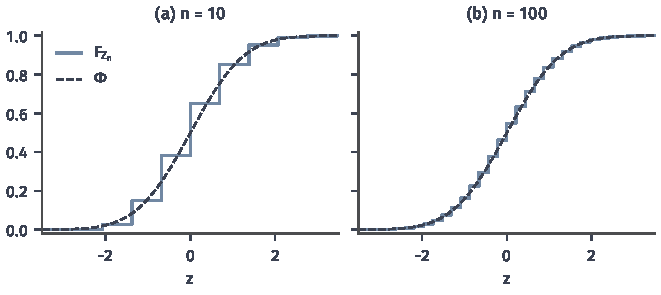
\includegraphics[width=112mm]{figures/01-basic-mathematics/05-probability-and-statistics-basics/matplotlib/samp-bernoulli-clt/figure.pdf}
  \caption{Bernoulli标准化和的分布函数与标准正态分布函数的对照。$S_n\sim\operatorname{Bin}(n,0.3)$，$Z_n=(S_n-0.3n)/\sqrt{0.21n}$；实线阶梯为$Z_n$的精确分布函数，虚线为$\Phi$。(a) $n=10$；(b) $n=100$。$n$增大时台阶变密、变低，阶梯逐渐贴近$\Phi$。}
  \label{fig:samp-bernoulli-clt}
\end{figure}

\begin{example}[平均服务时间]
\label{ex:samp-exponential-clt}
设$50$位顾客的服务时间独立同分布于率参数为$1$的指数分布（单位：分钟），$\mu=\sigma=1$。平均服务时间超过$1.2$分钟的概率约为
\[
  \mathbb{P}(\bar X_{50}>1.2)=\mathbb{P}\bigl(Z_{50}>\sqrt{50}\cdot0.2\bigr)\approx1-\Phi(1.414)\approx0.079.
\]
这里可以与精确值比较：$50\bar X_{50}$服从$\operatorname{Gamma}(50,1)$，精确概率约为$0.084$。指数分布明显右偏，$n=50$时近似已有用，但右尾仍被低估了一点。
\end{example}

\subsection{未知方差下的标准化}

\paragraph{用样本标准差替代}
式~\eqref{eq:samp-standardized-mean}需要已知$\sigma$。实际中我们只能计算
\[
  T_n=\frac{\sqrt n(\bar X_n-\mu)}{S_n}=Z_n\cdot\frac{\sigma}{S_n}.
\]
由定理~\ref{thm:samp-moment-consistency}，在有限方差下$S_n^2\xrightarrow{\mathbb{P}}\sigma^2$，再由引理~\ref{lem:samp-continuous-mapping}，$S_n/\sigma\xrightarrow{\mathbb{P}}1$。
直觉上，$n$大时乘以一个几乎等于$1$的随机因子不会改变极限分布。下面用高概率事件上的夹逼把这一直觉写成证明。

\begin{theorem}[用样本标准差标准化]
\label{thm:samp-studentized-clt}
设$X_1,X_2,\dots$独立同分布，均值$\mu$，方差$0<\sigma^2<\infty$。则$T_n=\sqrt n(\bar X_n-\mu)/S_n\xrightarrow{\mathrm{d}}\mathcal N(0,1)$。
\end{theorem}

\begin{proof}
固定$x\in\mathbb{R}$与$\delta\in(0,1)$。令$A_n=\{|S_n/\sigma-1|<\delta\}$，由$S_n/\sigma\xrightarrow{\mathbb{P}}1$，$\mathbb{P}(A_n^{\mathsf c})\to0$。

在$A_n$上$S_n>0$，且$\{T_n\leq x\}=\{Z_n\leq xS_n/\sigma\}$。这时$S_n/\sigma\in(1-\delta,1+\delta)$，所以$xS_n/\sigma$落在$x(1-\delta)$与$x(1+\delta)$之间。记这两个数中较小者为$x_-$，较大者为$x_+$（$x$为负时二者的次序与$x$为正时相反），则在$A_n$上
\[
  \{Z_n\leq x_-\}\subseteq\{T_n\leq x\}\subseteq\{Z_n\leq x_+\}.
\]
把这两个包含关系分别与$A_n$取交，再计入$A_n^{\mathsf c}$的概率，得到
\[
  \mathbb{P}(Z_n\leq x_-)-\mathbb{P}(A_n^{\mathsf c})\leq\mathbb{P}(T_n\leq x)\leq\mathbb{P}(Z_n\leq x_+)+\mathbb{P}(A_n^{\mathsf c}).
\]
令$n\to\infty$，由中心极限定理与$\mathbb{P}(A_n^{\mathsf c})\to0$，$\mathbb{P}(T_n\leq x)$的所有极限点都落在$[\Phi(x_-),\Phi(x_+)]$中。
再令$\delta\to0$，$x_\pm\to x$，由$\Phi$的连续性，上下两端都趋于$\Phi(x)$。所以$\mathbb{P}(T_n\leq x)\to\Phi(x)$。
\end{proof}

证明只用到两件事：$Z_n$的极限分布函数连续，以及替换因子依概率收敛到$1$。它没有用到$\bar X_n$与$S_n$独立，这一点很重要，因为示例~\ref{ex:samp-bernoulli-mean-variance-dependent}说明一般总体下两者并不独立。
同样的夹逼论证适用于“依分布收敛的量乘以或加上依概率收敛到常数的量”，这一般形式称为\term{Slutsky定理}（Slutsky's theorem）。

\paragraph{精确结果与渐近结果}
现在同一个统计量$T_n=\sqrt n(\bar X_n-\mu)/S_n$有了两种结论，它们的条件和含义不同。
\begin{itemize}
  \item 总体为正态时，由式~\eqref{eq:samp-t-statistic}，对每个$n\geq2$都有$T_n\sim t_{n-1}$，这是精确的有限样本结论。
  \item 总体只需方差有限时，由定理~\ref{thm:samp-studentized-clt}，$T_n$的分布在$n\to\infty$时趋于$\mathcal N(0,1)$，这是渐近结论，对固定的$n$只是近似。
\end{itemize}
两者在大样本下相容：示例~\ref{ex:samp-t-quantiles}的表中$t_{n-1,0.975}$随$n$增大趋于$1.96$。
小样本时，若有理由相信总体接近正态，用$t$分布更准确；若总体明显非正态，$t$分布不再精确，正态近似又可能尚未生效，此时两个结论都需要谨慎使用。

\subsection{正态近似的适用范围}
\label{sec:samp-normal-approximation-range}

\paragraph{偏斜、尾部与离散性}
中心极限定理不说明逼近多快。影响逼近速度的主要因素有三个。

总体越偏斜，需要的样本量越大。图~\ref{fig:samp-normal-approximation-range}(a)画出了指数总体标准化均值的精确密度：$n=1$时就是平移的指数密度，在$z=-1$处有一个跳跃；$n=5$时峰偏左、右尾偏长；$n=30$时已接近正态，但仍可看出左右不对称。
这种不对称使两侧尾部的近似误差不同：$n=5$时，右尾概率$\mathbb{P}(\bar X_5>1.5)$的精确值与正态近似都约为$0.132$，几乎相同；而对称位置的左尾概率$\mathbb{P}(\bar X_5<0.5)$精确值约为$0.109$，正态近似仍给出$0.132$。正态近似总是把两侧尾部看成一样大，偏斜总体做不到这一点。

总体尾部越重，样本中偶尔出现的极端值对均值影响越大，逼近也越慢；方差无限时定理根本不适用。

总体离散时，$S_n$只取整数，分布函数是阶梯，而$\Phi$是光滑曲线，图~\ref{fig:samp-bernoulli-clt}中的误差主要就出现在台阶的跳跃处。

\begin{figure}[htbp]
  \centering
  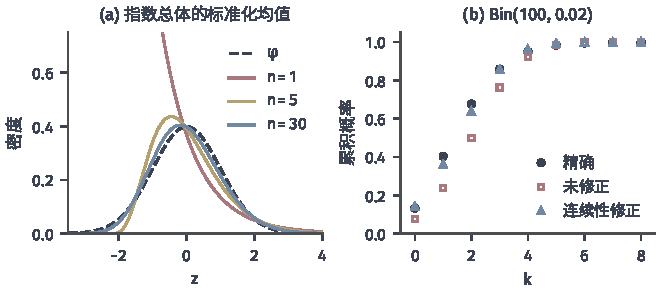
\includegraphics[width=112mm]{figures/01-basic-mathematics/05-probability-and-statistics-basics/matplotlib/samp-normal-approximation-range/figure.pdf}
  \caption{正态近似的效果取决于总体形状。(a) 率参数为$1$的指数总体下标准化均值$\sqrt n(\bar X_n-1)$的精确密度（由Gamma分布计算），$n=1,5,30$，虚线为标准正态密度$\varphi$；(b) $S\sim\operatorname{Bin}(100,0.02)$时$\mathbb{P}(S\leq k)$的精确值、未修正的正态近似与连续性修正后的近似。}
  \label{fig:samp-normal-approximation-range}
\end{figure}

\paragraph{连续性修正}
对取整数值的$S_n$，事件$\{S_n\leq k\}$与$\{S_n\leq k+\tfrac12\}$相同，与$\{S_n\leq k+0.99\}$也相同，但把它们分别代入式~\eqref{eq:samp-clt-approximation}会得到不同的近似值。
取中点$k+\tfrac12$，相当于把每个整数$j$的概率看作区间$(j-\tfrac12,j+\tfrac12]$上正态密度的面积，这称为\term{连续性修正}（continuity correction）：
\[
  \mathbb{P}(S_n\leq k)\approx\Phi\Bigl(\frac{k+\frac12-n\mu}{\sigma\sqrt n}\Bigr).
\]

\begin{example}[连续性修正的效果]
\label{ex:samp-continuity-correction}
设$S\sim\operatorname{Bin}(100,0.3)$，$np=30$，$\sqrt{np(1-p)}=\sqrt{21}\approx4.58$。精确值$\mathbb{P}(S\leq25)\approx0.163$。
不修正时近似为$\Phi\bigl((25-30)/4.58\bigr)=\Phi(-1.09)\approx0.138$；修正后为$\Phi\bigl((25.5-30)/4.58\bigr)=\Phi(-0.98)\approx0.163$，几乎与精确值相同。

再看偏斜的$S\sim\operatorname{Bin}(100,0.02)$，$np=2$，$\sqrt{np(1-p)}=1.4$。精确值$\mathbb{P}(S\geq5)=1-\mathbb{P}(S\leq4)\approx0.051$；
连续性修正后的近似为$1-\Phi\bigl((4.5-2)/1.4\bigr)\approx0.037$，不修正时为$1-\Phi\bigl((5-2)/1.4\bigr)\approx0.016$。
连续性修正改善了离散性带来的误差，却不能消除偏斜带来的误差，如图~\ref{fig:samp-normal-approximation-range}(b)所示。这时直接计算二项概率更可靠。
\end{example}

\paragraph{不能套用定理的情形}
常听到的“$n\geq30$即可用正态近似”只是经验说法，不是定理。
上例中$n=100$仍不够，因为有效的信息量取决于$np$而不是$n$；对更偏斜或尾部更重的总体，需要的样本量还会更大。
一个固定的样本量门槛不能对所有总体统一保证近似精度，使用时应检查数据的偏斜和极端值，有条件时与精确计算或模拟结果比较。

中心极限定理的两个条件也不能随意放宽。
第一，方差必须有限：标准Cauchy总体没有均值和方差，图~\ref{fig:samp-running-means}(b)中的样本均值始终不稳定，标准化更无从谈起。
第二，观测必须独立：若$X_1\sim\operatorname{Bernoulli}(1/2)$且$X_2=X_3=\dots=X_1$，则每个$\bar X_n=X_1$只取$0,1$两个值，无论$n$多大都不会接近正态。
存在依赖时，均值的方差不再是$\sigma^2/n$，有时也可以建立正态近似，但需要另外的条件，不能直接套用本节定理。

\section{本章小结}
\label{sec:samp-summary}

本章开头的问题是：按同一规则重复抽样时，估计会波动多少，样本增加后会怎样。
第一节把它落实为统计量的抽样分布，用标准误描述波动，用偏差描述系统偏离，用均方误差把两者合在一起；示例说明，无偏既不保证单次结果接近真值，也不保证均方误差最小。
其后三节给出了三类说明误差大小的依据，下表按成立条件、结果形式和所能回答的问题加以比较。

\begin{center}
\small
\begin{tabularx}{\linewidth}{>{\raggedright\arraybackslash}p{4.6em}>{\raggedright\arraybackslash}X>{\raggedright\arraybackslash}X>{\raggedright\arraybackslash}X}
\toprule
依据 & 成立条件 & 结果形式 & 能回答的问题 \\
\midrule
精确抽样分布 & 正态总体，独立同分布；样本量任意 & $\bar X_n$、$S_n^2$的分布及卡方、$t$、$F$统计量的精确分布 & 给定样本量下误差落在某范围内的确切概率 \\
有限样本概率界 & 只需均值或方差（或其上界）已知；样本量任意 & Markov、Chebyshev上界，如$\sigma^2/(n\varepsilon^2)$ & 保证失败概率不超过某值所需的样本量；结论偏保守 \\
渐近近似 & 独立同分布，方差有限；样本量趋于无穷 & 依概率收敛（大数定律、一致性）与依分布收敛（中心极限定理） & 大样本下估计是否趋于目标、误差的近似分布；有限样本精度需另行检查 \\
\bottomrule
\end{tabularx}
\end{center}

三类依据并不互相替代。精确分布最准确，但正态假设不成立时可能失效；概率界最稳健，但常常过于宽松；渐近近似适用面广且结论具体，却只在样本量足够大时可靠，而“足够大”取决于总体的偏斜、尾部和离散性。
用样本标准差代替总体标准差时，正态模型给出精确的$t$分布，一般总体则依靠一致性与Slutsky型替换得到渐近正态。

第~\ref{chap:intervals-tests-prediction}章将在这些依据上构造推断方法：正态均值与方差的区间和检验使用$t$、卡方与$F$分布；大样本的比例与均值区间使用中心极限定理和标准误估计；需要无分布假设的严格保证时，可以回到Chebyshev型的概率界。

\chapter{区间估计、假设检验与预测}
\label{chap:intervals-tests-prediction}

一台灌装机的标称灌装量是$500$ mL。质检员随机抽取$10$瓶，测得平均灌装量$501.5$ mL。第~\ref{chap:sample-estimation}章告诉我们怎样由样本得到这个点估计，第~\ref{chap:sampling-errors}章告诉我们样本均值在重复抽样中会波动多少。但实际工作提出的往往是另外三类问题：真正的平均灌装量大致在什么范围内？“平均灌装量就是$500$ mL”这个说法与数据是否相容？下一瓶会装多少？

这三个问题分别对应本章的三项统计任务：用区间圈定未知参数，用检验判断关于参数的陈述，用区间预测尚未观测的结果。它们使用的原料相同，都是统计量的抽样分布或参数的后验分布；差别在于所要覆盖或判断的对象不同，因而概率的含义也不同。第~\ref{sec:pred-intervals}节先构造均值、比例和方差的区间，并把后验可信区间与之比较；第~\ref{sec:pred-tests}节建立检验的共同概念，再按参数逐一构造检验，最后说明检验与区间如何互相转化；第~\ref{sec:pred-prediction}节把对象换成未来观测，说明预测区间为什么总比均值区间宽；第~\ref{sec:pred-regression}节在简单线性回归中把估计、区间、检验与预测放进同一个模型。

全章反复使用一组教学数据，便于比较不同方法对同一问题给出的回答。

\begin{example}[灌装量数据]
\label{ex:pred-filling-data}
从灌装机A随机抽取$10$瓶，灌装量（单位：mL，教学数据）为
\[
 501.8,\ 499.6,\ 502.4,\ 500.9,\ 503.1,\ 501.2,\ 499.9,\ 502.6,\ 501.5,\ 502.0.
\]
样本均值$\bar x=5015/10=501.5$。各观测与均值之差的平方和为$\sum_i(x_i-\bar x)^2=11.54$，于是修正样本方差$s^2=11.54/9\approx1.2822$，样本标准差$s\approx1.1324$，均值的估计标准误$s/\sqrt{10}\approx0.3581$。本章把这批数据看作正态总体$\mathcal N(\mu,\sigma^2)$的独立样本，除非另有说明。
\end{example}

本章沿用前几章的记号：$\Phi$是标准正态分布函数，$z_p=\Phi^{-1}(p)$是其下侧$p$分位数；$t_{k,p}$、$\chi^2_{k,p}$、$F_{k_1,k_2,p}$分别是自由度为$k$的$t$分布、卡方分布以及自由度为$(k_1,k_2)$的$F$分布的下侧$p$分位数。样本$X_1,\dots,X_n$的样本均值记$\bar X_n$，修正样本方差记$S_n^2$；不致混淆时省略下标$n$。参数为$\theta$时计算的概率与期望记作$\mathbb P_\theta$与$\mathbb E_\theta$。

\section{区间估计}
\label{sec:pred-intervals}

点估计$\bar x=501.5$没有告诉我们它离真值可能有多远。第~\ref{sec:samp-standard-error}节用标准误描述了估计量的典型波动幅度；本节更进一步，把这种波动换算成一个区间，并要求这个区间在重复抽样中以指定的概率覆盖真参数。我们先说明覆盖概率的含义和一般构造方法，再依次处理均值、比例与方差，最后把这些区间与由后验分布得到的区间相比较。

\subsection{置信区间与覆盖率}

\paragraph{区间端点是统计量}

设想质检员每天都抽$10$瓶、每天都报一个区间。今天的区间是由今天的样本算出来的，明天换一批样本，区间也随之改变。因此在抽样之前，区间的两个端点是样本的函数，即两个统计量；而要估计的平均灌装量$\mu$是一个固定但未知的数。说一个区间“可靠”，只能是说这种构造规则在反复使用时多半能把$\mu$圈住。

\begin{definition}[置信区间]
\label{def:pred-confidence-interval}
设样本$\bm X=(X_1,\dots,X_n)$的分布由参数$\theta\in\Theta$决定，$L(\bm X)\leq U(\bm X)$是两个统计量，$0<\alpha<1$。函数
\[
 C(\theta)=\mathbb P_\theta\bigl(L(\bm X)\leq\theta\leq U(\bm X)\bigr),\qquad\theta\in\Theta,
\]
称为随机区间$[L(\bm X),U(\bm X)]$的\term{覆盖概率}（coverage probability）。若对每个$\theta\in\Theta$都有$C(\theta)\geq1-\alpha$，则称$[L(\bm X),U(\bm X)]$为$\theta$的置信水平为$1-\alpha$的\term{置信区间}（confidence interval），$1-\alpha$称为\term{置信水平}（confidence level）。
\end{definition}

定义里的概率是对样本$\bm X$计算的，$\theta$在概率符号中只作为分布的标号出现。要求“对每个$\theta$”成立，是因为我们不知道真参数是哪一个，只能要求构造规则无论面对哪个参数都可靠。只允许取一侧的区间，例如$(-\infty,U(\bm X)]$，同样可以按此定义，称为单侧置信区间或置信上界。

一旦代入观测值，例如例~\ref{ex:pred-filling-t-interval}将由灌装量数据算得区间$[500.69,502.31]$，它就是两个确定的数。这时$\mu$要么在其中，要么不在，“$\mu$以$95\%$的概率落在$[500.69,502.31]$中”不是置信区间所能支持的说法；$95\%$描述的是产生这个区间的规则。图~\ref{fig:pred-coverage-simulation}把这种规则重复执行了$50$次：每次从同一个正态总体抽$10$个观测并按下文的$t$区间公式计算，大多数区间穿过真值所在的虚线，少数区间整个落在虚线一侧。

\begin{figure}[htbp]
  \centering
  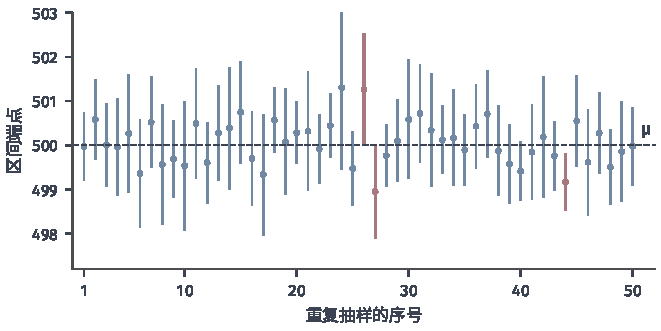
\includegraphics[width=112mm]{figures/01-basic-mathematics/05-probability-and-statistics-basics/matplotlib/pred-coverage-simulation/figure.pdf}
  \caption{同一构造规则的$50$次重复。每次从$\mathcal N(500,1.5^2)$独立抽取$10$个观测，计算$95\%$的$t$区间（竖线）与样本均值（圆点）；虚线是真均值$\mu=500$。红色的$3$个区间未覆盖真值，其余$47$个覆盖。区间的中心与长度都随样本变化，真值固定不动。模拟使用固定随机种子$20261028$。}
  \label{fig:pred-coverage-simulation}
\end{figure}

\paragraph{从标准化量反解参数}

怎样得到覆盖概率可控的区间？关键是找一个同时含样本与参数、而分布与参数无关的量。最简单的例子来自第~\ref{sec:samp-normal}节：正态样本且$\sigma$已知时，
\[
 Z=\frac{\bar X-\mu}{\sigma/\sqrt n}\sim\mathcal N(0,1),
\]
无论$\mu$取什么值，$Z$都服从标准正态分布。

\begin{definition}[枢轴量]
\label{def:pred-pivot}
若$Q(\bm X,\theta)$的分布在每个$\mathbb P_\theta$下都相同、不依赖$\theta$，则称$Q$为\term{枢轴量}（pivotal quantity）。
\end{definition}

有了枢轴量，构造分两步。第一步取其分布的两个分位数$q_{\alpha/2}$与$q_{1-\alpha/2}$，使$\mathbb P_\theta(q_{\alpha/2}\leq Q\leq q_{1-\alpha/2})=1-\alpha$对一切$\theta$成立；第二步把不等式$q_{\alpha/2}\leq Q(\bm X,\theta)\leq q_{1-\alpha/2}$对$\theta$解出来。若解集是一个区间$[L(\bm X),U(\bm X)]$，则两个事件相同，覆盖概率恰为$1-\alpha$。以$Z$为例，
\[
 -z_{1-\alpha/2}\leq\frac{\bar X-\mu}{\sigma/\sqrt n}\leq z_{1-\alpha/2}
 \iff
 \bar X-z_{1-\alpha/2}\frac{\sigma}{\sqrt n}\leq\mu\leq\bar X+z_{1-\alpha/2}\frac{\sigma}{\sqrt n},
\]
其中用到标准正态分布关于零对称，$z_{\alpha/2}=-z_{1-\alpha/2}$。本节后面的均值、方差区间都按这条路线构造，差别只在于枢轴量不同。

\paragraph{名义覆盖率、实际覆盖率与区间长度}

构造时要求的$1-\alpha$称为\term{名义覆盖率}（nominal coverage），覆盖概率$C(\theta)$的实际数值称为实际覆盖率。若枢轴量的分布准确已知，二者相等；若只用了近似分布，或样本取值离散，实际覆盖率可能低于或高于名义值，并且可能随$\theta$变化。评价一个区间方法，首先看实际覆盖率是否至少接近名义值。

覆盖率并不是唯一标准。区间$(-\infty,\infty)$的覆盖率永远是$1$，却没有提供任何信息。所以在覆盖率达到要求的方法中，我们希望区间尽量短。对同一个枢轴量，提高置信水平会换用更外侧的分位数，区间随之变长；增加样本量则通过$1/\sqrt n$缩短区间。下文比较不同方法时，总是同时看覆盖率与长度这两项。

\subsection{均值的置信区间}

均值区间按总体的已知程度分三种情形：正态且方差已知、正态而方差未知、只知道方差有限。前两种有精确的枢轴量，第三种只能依靠大样本近似。

\paragraph{正态总体、方差已知}

若$X_1,\dots,X_n$独立同分布于$\mathcal N(\mu,\sigma^2)$且$\sigma$已知，上一小节已经从$Z$得到
\begin{equation}
 \bar X\pm z_{1-\alpha/2}\frac{\sigma}{\sqrt n}.
 \label{eq:pred-z-interval}
\end{equation}
它的覆盖概率对每个$\mu$都恰好是$1-\alpha$，长度$2z_{1-\alpha/2}\sigma/\sqrt n$不随样本变化。

\begin{example}[方差已知时的灌装量区间]
\label{ex:pred-filling-z-interval}
假定设备手册给出灌装量的标准差$\sigma=1.5$ mL，并信任这一数值。对例~\ref{ex:pred-filling-data}，$95\%$置信区间为
\[
 501.5\pm1.96\times\frac{1.5}{\sqrt{10}}=501.5\pm0.930=[500.57,\,502.43].
\]
\end{example}

\paragraph{正态总体、方差未知：$t$区间}

实际中$\sigma$通常未知，自然的做法是用$S$代替它。代替后的量不再服从标准正态分布：分母也随样本波动，尾部会更厚。第~\ref{sec:samp-normal}节证明了，正态样本的$\bar X$与$S^2$相互独立，且$(n-1)S^2/\sigma^2\sim\chi^2_{n-1}$；第~\ref{sec:samp-t}节由此得到
\begin{equation}
 T=\frac{\bar X-\mu}{S/\sqrt n}\sim t_{n-1}.
 \label{eq:pred-t-pivot}
\end{equation}
$T$的分布不含$\mu$与$\sigma$，是枢轴量。$t$分布关于零对称，按同样的反解得到\term{$t$区间}（$t$ interval）
\begin{equation}
 \bar X\pm t_{n-1,1-\alpha/2}\frac{S}{\sqrt n}.
 \label{eq:pred-t-interval}
\end{equation}
对正态总体，它的覆盖概率对一切$(\mu,\sigma^2)$恰为$1-\alpha$。

$t$分位数总大于对应的正态分位数，这是为$\sigma$的估计误差付出的代价：$t_{2,0.975}\approx4.303$，$t_{4,0.975}\approx2.776$，$t_{9,0.975}\approx2.262$，$t_{29,0.975}\approx2.045$，$t_{99,0.975}\approx1.984$，随自由度增大逐渐接近$z_{0.975}\approx1.960$。小样本时差别显著，样本数十以上时差别已不大。

\begin{example}[方差未知时的灌装量区间]
\label{ex:pred-filling-t-interval}
不再假定$\sigma$已知。对例~\ref{ex:pred-filling-data}，$t_{9,0.975}\approx2.262$，估计标准误$s/\sqrt{10}\approx0.3581$，故$95\%$的$t$区间为
\[
 501.5\pm2.262\times0.3581=501.5\pm0.810=[500.69,\,502.31].
\]
这个区间反而比例~\ref{ex:pred-filling-z-interval}窄，原因是这批样本的$s\approx1.13$恰好小于手册给出的$\sigma=1.5$。在重复抽样的平均意义下，$t$区间比已知$\sigma$时的区间长；对一个具体样本，二者谁长取决于$s$的大小。
\end{example}

\paragraph{一般总体的大样本区间}

总体不是正态时，$T$不再精确服从$t_{n-1}$。若$X_1,\dots,X_n$独立同分布，方差$\sigma^2$有限且大于零，第~\ref{sec:samp-clt}节的中心极限定理说明$\sqrt n(\bar X_n-\mu)/\sigma$的分布函数逐点收敛于$\Phi$；第~\ref{sec:samp-consistency}节又说明$S_n$依概率收敛于$\sigma$。把分母中的$\sigma$换成$S_n$相当于乘上一个依概率趋于$1$的因子$\sigma/S_n$，第~\ref{sec:samp-clt}节用Slutsky定理说明了这种替换不改变极限分布。于是对每个固定的总体分布，
\[
 \lim_{n\to\infty}\mathbb P\Bigl(\Bigl|\frac{\bar X_n-\mu}{S_n/\sqrt n}\Bigr|\leq z_{1-\alpha/2}\Bigr)=1-\alpha,
\]
区间$\bar X_n\pm z_{1-\alpha/2}S_n/\sqrt n$的覆盖概率趋于名义值。实际中常用$t$分位数代替$z_{1-\alpha/2}$，两者在大样本下几乎相同，而$t$分位数在小样本时略为保守。

这个结论是渐近性质：它说的是$n\to\infty$时的极限，并不保证某个固定的$n$已经足够，也不保证收敛对所有总体同样快。总体越偏斜，需要的样本量越大。

\begin{example}[偏斜总体下的$t$区间]
\label{ex:pred-exponential-coverage}
设总体是均值为$1$的指数分布。用固定随机种子$20261028$各重复$200000$次，名义$95\%$的$t$区间的实际覆盖率约为：$n=5$时$0.88$，$n=10$时$0.90$，$n=30$时$0.93$，$n=100$时$0.94$。覆盖率随$n$增大而逼近$0.95$，但小样本时明显不足。未覆盖的情形也不对称：$n=10$时约$9.6\%$的区间整个落在真均值左侧，只有约$0.4\%$落在右侧。指数分布右偏：样本中没有出现大观测时，样本均值偏低，样本标准差也偏小，区间又低又短，于是整个落在真均值左侧；出现大观测时样本均值偏高，但样本标准差同时变大，区间很宽，往往仍能覆盖真值。
\end{example}

\subsection{比例的置信区间}

\paragraph{正态近似区间}

灌装线上的另一项指标是封口不合格率$p$。把第$i$瓶不合格记为$X_i=1$、合格记为$X_i=0$，则$X_i\sim\operatorname{Bernoulli}(p)$，不合格数$S=\sum_iX_i\sim\operatorname{Bin}(n,p)$，样本比例$\hat p=S/n$就是样本均值。于是比例的区间是均值区间的特例：Bernoulli总体的方差为$p(1-p)$，用$\hat p(1-\hat p)$估计它，大样本区间成为
\begin{equation}
 \hat p\pm z_{1-\alpha/2}\sqrt{\frac{\hat p(1-\hat p)}{n}}.
 \label{eq:pred-wald-interval}
\end{equation}
这个区间称为\term{Wald区间}（Wald interval）。它只依赖中心极限定理，因此只是近似区间。

\begin{example}[封口不合格率的Wald区间]
\label{ex:pred-wald}
抽查$n=40$瓶，发现$s=6$瓶封口不合格，$\hat p=0.15$。估计标准误$\sqrt{0.15\times0.85/40}\approx0.0565$，$95\%$的Wald区间为$0.15\pm1.96\times0.0565=[0.039,\,0.261]$。

再看一个极端情形：抽查$n=20$瓶，全部合格，$s=0$。这时$\hat p=0$，估计标准误也是$0$，式~\eqref{eq:pred-wald-interval}给出单点区间$[0,0]$，等于断言不合格率恰好为零。这显然过于自信。
\end{example}

例中的退化并非偶然。Wald区间有两处近似：用正态分布近似离散的二项分布，以及用$\hat p$代替标准误中的$p$。当$n$不大或$p$接近$0$、$1$时，二项分布明显偏斜，两处近似都不可靠。图~\ref{fig:pred-proportion-coverage}按二项概率精确计算了$n=30$时Wald区间的覆盖概率：在中间区域它多数时候低于$0.95$，并随$p$锯齿状跳动；靠近边界时覆盖率急剧下降，$p=0.05$处约为$0.78$。

\begin{figure}[htbp]
  \centering
  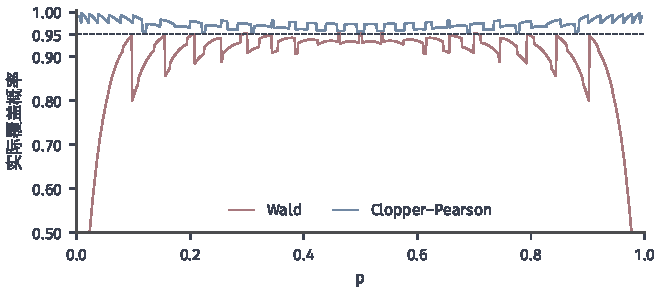
\includegraphics[width=112mm]{figures/01-basic-mathematics/05-probability-and-statistics-basics/matplotlib/pred-proportion-coverage/figure.pdf}
  \caption{$n=30$时两种名义$95\%$比例区间的实际覆盖概率，按$C(p)=\sum_{s}\mathbb P_p(S=s)\,\mathbb I_{\{p\in[L(s),U(s)]\}}$精确计算。红线为Wald区间，在大部分$p$处低于虚线$0.95$，靠近$0$与$1$时急剧下降；蓝线为Clopper--Pearson区间，处处不低于$0.95$，多数位置明显高于它。锯齿来自$S$只能取整数。}
  \label{fig:pred-proportion-coverage}
\end{figure}

图中的锯齿说明了离散分布的一个特点。$S$只取$0,1,\dots,n$这$n+1$个值，因此区间也只有$n+1$个可能的结果。$p$连续变化时，某个$s$对应的区间端点一旦越过$p$，这个$s$的概率就整块进入或离开覆盖概率，覆盖率随之跳动。

\paragraph{由二项尾概率反求：精确区间}

既然问题出在近似，我们改为直接使用二项分布。思路是：观测到$s$之后，把那些“使观测值落在过远尾部”的$p$排除掉。若$p$很小，出现$s$或更多不合格的概率$\mathbb P_p(S\geq s)$就很小；若$p$很大，出现$s$或更少的概率$\mathbb P_p(S\leq s)$很小。两侧各留$\alpha/2$，即得下面的区间。

\begin{definition}[Clopper--Pearson区间]
\label{def:pred-clopper-pearson}
设$S\sim\operatorname{Bin}(n,p)$，观测值为$s$。当$s\geq1$时，令$p_L(s)$为方程$\mathbb P_p(S\geq s)=\alpha/2$关于$p$的解；当$s=0$时，令$p_L(0)=0$。当$s\leq n-1$时，令$p_U(s)$为方程$\mathbb P_p(S\leq s)=\alpha/2$关于$p$的解；当$s=n$时，令$p_U(n)=1$。区间$[p_L(S),p_U(S)]$称为\term{Clopper--Pearson区间}（Clopper--Pearson interval），也称精确区间。
\end{definition}

定义中的方程有唯一解，依据是二项尾概率关于$p$的单调性：对固定的$s\geq1$，$\mathbb P_p(S\geq s)$随$p$严格增加，从$p=0$时的$0$连续增到$p=1$时的$1$。直观上，成功概率越大，成功次数越容易达到$s$。严格的说明可以用一个耦合构造：取$U_1,\dots,U_n$独立同分布于$\operatorname U(0,1)$，令$S_p=\sum_i\mathbb I_{\{U_i\leq p\}}$，则$S_p\sim\operatorname{Bin}(n,p)$；当$p<p'$时每一项$\mathbb I_{\{U_i\leq p\}}\leq\mathbb I_{\{U_i\leq p'\}}$，故$S_p\leq S_{p'}$，从而$\mathbb P(S_p\geq s)\leq\mathbb P(S_{p'}\geq s)$。这说明了单调不减。至于严格增加与连续性，$\mathbb P_p(S\geq s)=\sum_{k\geq s}\binom nk p^k(1-p)^{n-k}$是$p$的多项式，逐项求导后相邻项相消，只剩$n\binom{n-1}{s-1}p^{s-1}(1-p)^{n-s}$，它在$0<p<1$上为正。同理，$\mathbb P_p(S\leq s)$随$p$严格减少。

\begin{theorem}[Clopper--Pearson区间的覆盖]
\label{thm:pred-clopper-pearson-coverage}
对每个$p\in[0,1]$，都有
\[
 \mathbb P_p\bigl(p_L(S)\leq p\leq p_U(S)\bigr)\geq1-\alpha.
\]
\end{theorem}

\begin{proof}
固定真参数$p$，只需证明区间漏掉$p$的两种情形各自的概率小于$\alpha/2$。对整数$s$，记尾概率$g(s)=\mathbb P_p(S\geq s)$，这里$p$是固定的真参数。先看$p<p_L(s)$在哪些$s$上发生。$s=0$时$p_L=0$，不会发生；$s\geq1$时，$p_L(s)$是方程$\mathbb P_{p'}(S\geq s)=\alpha/2$关于$p'$的解，而左边随$p'$严格增加，所以$p<p_L(s)$当且仅当$g(s)<\alpha/2$。又$g(s)$随$s$递减，满足$g(s)<\alpha/2$的$s$构成一个右端集合$\{s:s\geq s^*\}$，其中$s^*$是使$g(s)<\alpha/2$的最小整数（若不存在，此情形概率为$0$）。于是
\[
 \mathbb P_p\bigl(p<p_L(S)\bigr)=\mathbb P_p(S\geq s^*)=g(s^*)<\frac\alpha2.
\]
对$p>p_U(S)$作对称的论证，得到其概率也小于$\alpha/2$。两种情形互斥，漏掉$p$的概率小于$\alpha$。
\end{proof}

证明的最后一步只能得到“小于$\alpha/2$”而不是“等于”，正是离散性所致：$g(s^*)$是尾概率函数在整数点上的取值，一般不会恰好落在$\alpha/2$上。因此Clopper--Pearson区间是\emph{保守}的，实际覆盖率通常高于名义值。图~\ref{fig:pred-proportion-coverage}中的蓝线显示了这一点：覆盖率处处不低于$0.95$，多数位置在$0.96$以上，靠近边界时接近$1$。保守换来的代价是区间较长。

计算上，$p_L$与$p_U$可以用Beta分布的分位数表示：$p_L(s)$是$\operatorname{Beta}(s,n-s+1)$的$\alpha/2$分位数，$p_U(s)$是$\operatorname{Beta}(s+1,n-s)$的$1-\alpha/2$分位数。这来自恒等式$\mathbb P_p(S\geq s)=\mathbb P(B\leq p)$，其中$B\sim\operatorname{Beta}(s,n-s+1)$：上面求得的导数$n\binom{n-1}{s-1}p^{s-1}(1-p)^{n-s}$恰是$\operatorname{Beta}(s,n-s+1)$的密度，两边在$p=0$处又都为$0$。

\begin{example}[两种比例区间的比较]
\label{ex:pred-clopper-pearson}
对$n=40$、$s=6$，Clopper--Pearson区间约为$[0.057,\,0.298]$，比Wald区间$[0.039,\,0.261]$长约$0.02$，并且整体右移：二项分布在$p$较小时右偏，精确区间把这种不对称保留下来。

对$n=20$、$s=0$，$p_L=0$，$p_U$满足$(1-p)^{20}=0.025$，解得$p_U=1-0.025^{1/20}\approx0.168$。区间$[0,\,0.168]$承认，即使$20$瓶全部合格，不合格率仍可能高达约$17\%$；Wald区间的$[0,0]$则完全忽略了这种可能。
\end{example}

两种区间各有用途。Wald区间形式简单，在$n\hat p$与$n(1-\hat p)$都较大时表现尚可；Clopper--Pearson区间在任何$n$下都保证覆盖率，适合样本小或比例接近边界的情形。实践中还有一些覆盖率更接近名义值、长度更短的折中方法，这里不展开。

\subsection{方差的置信区间}

灌装量的波动大小同样关系质量：均值合格而方差过大，仍会有许多瓶偏离标称。我们需要总体方差$\sigma^2$的区间。

\paragraph{卡方枢轴量}

第~\ref{sec:samp-chi-square}节证明，若$X_1,\dots,X_n$独立同分布于$\mathcal N(\mu,\sigma^2)$，则
\[
 \frac{(n-1)S^2}{\sigma^2}\sim\chi^2_{n-1}.
\]
这个量的分布不含$\mu$与$\sigma^2$，是枢轴量。取卡方分布的两个分位数，
\[
 \chi^2_{n-1,\alpha/2}\leq\frac{(n-1)S^2}{\sigma^2}\leq\chi^2_{n-1,1-\alpha/2}
 \iff
 \frac{(n-1)S^2}{\chi^2_{n-1,1-\alpha/2}}\leq\sigma^2\leq\frac{(n-1)S^2}{\chi^2_{n-1,\alpha/2}},
\]
其中对正数取倒数时不等号方向反转。于是$\sigma^2$的置信水平为$1-\alpha$的区间为
\begin{equation}
 \Bigl[\frac{(n-1)S^2}{\chi^2_{n-1,1-\alpha/2}},\ \frac{(n-1)S^2}{\chi^2_{n-1,\alpha/2}}\Bigr].
 \label{eq:pred-variance-interval}
\end{equation}
对两端开平方，就得到$\sigma$的区间，覆盖概率不变，因为平方根是严格增函数。

\begin{example}[灌装量方差的区间]
\label{ex:pred-filling-variance-interval}
对例~\ref{ex:pred-filling-data}，$(n-1)s^2=11.54$，$\chi^2_{9,0.025}\approx2.700$，$\chi^2_{9,0.975}\approx19.023$。$\sigma^2$的$95\%$置信区间为
\[
 \Bigl[\frac{11.54}{19.023},\ \frac{11.54}{2.700}\Bigr]\approx[0.607,\,4.273],
\]
相应$\sigma$的区间约为$[0.779,\,2.067]$。点估计$s^2\approx1.282$距左端点$0.675$，距右端点$2.991$。
\end{example}

例中的区间明显不对称，原因在于卡方分布右偏：它的左尾短、右尾长，两个分位数到中心的距离不同；而反解时又取了倒数，把右尾的长度转移到了区间的右端。这种不对称也符合直观：$\sigma^2$只能取正值，样本方差的误差更接近按比例发生，而不是按差值发生。例如样本方差只有真方差的一半，与样本方差是真方差的两倍，都是小样本中常见的偏离，前者对应的真值在点估计右侧$s^2$处，后者对应的真值在左侧$s^2/2$处，所以区间向右伸得更远。只有$10$个观测时，方差的区间宽到上下端点相差七倍，说明小样本几乎无法精确确定波动大小。

\paragraph{对正态性的依赖}

均值的$t$区间在非正态总体下至少还有大样本的保障，方差的卡方区间却没有。原因可以通过比较$S^2$的波动来看。由于$S^2$与$\frac1n\sum_i(X_i-\mu)^2$只差一个在大样本下可以忽略的项，后者又是独立同分布变量$(X_i-\mu)^2$的样本均值，按中心极限定理，$\sqrt n(S^2-\sigma^2)$近似服从均值为$0$、方差为$\operatorname{Var}\bigl((X-\mu)^2\bigr)=\mu_4-\sigma^4$的正态分布，其中$\mu_4=\mathbb E(X-\mu)^4$为四阶中心矩（这里假设它有限）。

卡方区间的长度是按正态总体设计的。正态总体的$\mu_4=3\sigma^4$，故上式方差为$2\sigma^4$；这与卡方结论相符，因为由$\chi^2_{n-1}$的方差$2(n-1)$得$\operatorname{Var}(S^2)=2\sigma^4/(n-1)$，乘以$n$后趋于$2\sigma^4$。若总体的$\mu_4$大于$3\sigma^4$，即尾部比正态厚，$S^2$的真实波动就大于卡方区间所预设的波动，区间偏短；而且这种偏差不随$n$增大而消失，因为两者的比值$(\mu_4-\sigma^4)/(2\sigma^4)$与$n$无关。

\begin{example}[指数总体下的方差区间]
\label{ex:pred-variance-nonnormal}
均值为$1$的指数分布有$\sigma^2=1$，$\mu_4=9$，$S^2$的大样本方差是正态情形的$(9-1)/2=4$倍，标准差是$2$倍。按上面的近似，卡方区间实际只覆盖$|N|\leq1.96/2$的情形，$N$为标准正态，故$n$很大时实际覆盖率趋于$2\Phi(0.98)-1\approx0.673$。模拟（种子$20261028$，各重复$200000$次）给出的实际覆盖率为：$n=5$时$0.82$，$n=10$时$0.77$，$n=30$时$0.71$，$n=100$时$0.69$。样本越多，覆盖率反而越接近这个偏低的极限。
\end{example}

所以方差区间~\eqref{eq:pred-variance-interval}的精确性完全建立在正态假设之上，不能以“样本量足够大”为理由用于非正态总体。使用前应当检查数据是否有明显的偏斜或厚尾。

\subsection{后验可信区间}

前面几小节把参数视为固定未知的数。第~\ref{sec:est-bayes}节介绍了另一种做法：给参数指定先验分布，观测数据后得到后验分布，后验分布直接描述了在当前信息下参数各种取值的可能性。由后验分布同样可以给出参数范围。

\paragraph{等尾可信区间}

后验分布已经给出了参数落在任意范围内的概率，因此只需挑选一个后验概率达到要求的区间。

\begin{definition}[可信区间]
\label{def:pred-credible-interval}
给定观测数据$\bm x$与参数$\theta$的后验分布。若区间$[a,b]$满足$\mathbb P(a\leq\theta\leq b\mid\bm x)=1-\alpha$，则称它为$\theta$的后验概率为$1-\alpha$的\term{可信区间}（credible interval）。取$a$、$b$分别为后验分布的$\alpha/2$与$1-\alpha/2$分位数，得到\term{等尾可信区间}（equal-tailed credible interval）。
\end{definition}

满足要求的区间不止一个；等尾区间两侧各留$\alpha/2$的后验概率，计算最简单。后验分布不对称时，也可以选取长度最短的区间，这里不展开。我们用第~\ref{sec:est-posterior}节的两个共轭模型计算等尾区间。

\begin{example}[不合格率的可信区间]
\label{ex:pred-beta-credible}
在Beta--Bernoulli模型中，先验$p\sim\operatorname{Beta}(a,b)$，观测$n$次中有$s$次成功后，后验为$\operatorname{Beta}(a+s,\,b+n-s)$。取均匀先验$\operatorname{Beta}(1,1)$，对例~\ref{ex:pred-wald}的$n=40$、$s=6$，后验为$\operatorname{Beta}(7,35)$，其$0.025$与$0.975$分位数约为$0.072$与$0.292$。因此$[0.072,\,0.292]$是$p$的$95\%$等尾可信区间：在均匀先验和观测数据下，$p$落在其中的后验概率为$0.95$。它与Clopper--Pearson区间$[0.057,\,0.298]$接近，但含义不同，下面再作比较。
\end{example}

\begin{example}[灌装量均值的可信区间]
\label{ex:pred-normal-credible}
设灌装量$X_i\mid\mu\sim\mathcal N(\mu,\sigma^2)$相互独立，$\sigma^2=2.25$已知，先验$\mu\sim\mathcal N(\mu_0,\tau_0^2)$。第~\ref{sec:est-posterior}节得到后验仍为正态：后验精度是先验精度与数据精度之和，
\[
 \frac1{\tau_n^2}=\frac1{\tau_0^2}+\frac n{\sigma^2},
\]
后验均值$\mu_n$是先验均值与样本均值按各自精度加权的平均，
\[
 \mu_n=\tau_n^2\Bigl(\frac{\mu_0}{\tau_0^2}+\frac{n\bar x}{\sigma^2}\Bigr).
\]
取$\mu_0=500$、$\tau_0=1$（相信设备大致按标称灌装），对例~\ref{ex:pred-filling-data}的$n=10$、$\bar x=501.5$，后验精度为$1+10/2.25\approx5.444$，$\tau_n^2\approx0.1837$，$\tau_n\approx0.429$，后验均值
\[
 \mu_n\approx0.1837\times\Bigl(500+\frac{10\times501.5}{2.25}\Bigr)\approx501.22.
\]
$95\%$等尾可信区间为$501.22\pm1.96\times0.429=[500.38,\,502.06]$。与例~\ref{ex:pred-filling-z-interval}的置信区间$[500.57,\,502.43]$相比，它略窄，中心向先验均值$500$收缩了约$0.28$。
\end{example}

\paragraph{两种概率含义的比较}

可信区间和置信区间都写成“参数在某个范围内”，但其中的概率来自不同的随机性。置信区间的$1-\alpha$是对样本计算的：参数固定，区间随样本变化，规则在重复抽样中以概率$1-\alpha$覆盖参数。可信区间的$1-\alpha$是对参数计算的：数据固定，参数按后验分布变化，它落在区间中的后验概率为$1-\alpha$。所以对一次观测得到的可信区间，可以说“在给定先验与模型下，$\mu$在$[500.38,502.06]$中的概率是$0.95$”；对置信区间则不能这样说。

反过来，可信区间也不自动具有置信区间的保证。把例~\ref{ex:pred-normal-credible}的构造规则当作一个频率方法来检验：真均值固定为$\mu$，反复抽样并每次计算可信区间，覆盖概率是多少？后验均值$\mu_n=w\mu_0+(1-w)\bar X$，其中$w=\tau_n^2/\tau_0^2\approx0.184$，因此$\mu_n-\mu=w(\mu_0-\mu)+(1-w)(\bar X-\mu)$服从均值为$w(\mu_0-\mu)$、标准差为$(1-w)\sigma/\sqrt n\approx0.387$的正态分布，其中均值就是偏差。覆盖概率是这个正态变量落在$[-1.96\tau_n,\,1.96\tau_n]=[-0.840,\,0.840]$中的概率，计算得真均值为$500$时覆盖率约$0.97$，为$501.5$时约$0.93$，为$503$时只有约$0.77$。先验越偏离真值，频率覆盖率越低。先验恰当时，可信区间提供了置信区间所不能给出的直接概率陈述；先验不恰当时，它的频率性质可能很差。样本量增大时，数据精度$n/\sigma^2$压倒先验精度，$w\to0$，两种区间趋于一致。

\section{假设检验}
\label{sec:pred-tests}

区间回答“参数大概在哪里”，而许多实际问题要求对一个具体陈述作出判断：灌装机的平均灌装量是不是标称的$500$ mL？新测量方法与旧方法是否有系统差异？不合格率是否超过了合同规定的$5\%$？\term{假设检验}（hypothesis testing）把这类陈述写成关于参数的假设，并规定在数据达到什么程度时否定它。

本节前三个小节建立所有检验共有的概念：如何表述假设与拒绝域，判断可能犯哪两类错误，以及怎样用$p$值报告证据的强弱。接着按待检验的参数，依次处理单总体均值、两总体均值、比例与方差。最后一个小节说明检验与置信区间其实是同一组构造的两种读法。

\subsection{原假设、备择假设与拒绝域}

\paragraph{把陈述写成参数集合}

对一个统计模型，参数集$\Theta$中的每个值描述一种可能的总体。关于总体的陈述，例如“平均灌装量等于$500$”，就对应$\Theta$的一个子集。检验总是在两个互不相交的子集之间作选择。

\begin{definition}[原假设与备择假设]
\label{def:pred-hypotheses}
设参数集$\Theta$被分成两个不相交的非空子集$\Theta_0$与$\Theta_1$。陈述$H_0:\theta\in\Theta_0$称为\term{原假设}（null hypothesis），$H_1:\theta\in\Theta_1$称为\term{备择假设}（alternative hypothesis）。若$\Theta_0$只含一个点，称$H_0$为简单假设，否则称为复合假设。
\end{definition}

两个假设的地位并不对称。检验的逻辑是：先假定$H_0$成立，再看数据是否与之明显矛盾；只有矛盾足够明显，才否定$H_0$，转而采纳$H_1$。因此$H_0$通常是“没有差异”“符合标准”这类默认陈述，而希望用数据证明的结论放在$H_1$中。

以灌装量均值$\mu$为例，按所关心的问题可以写出三种检验问题：
\begin{itemize}
  \item 只关心是否偏离标称：$H_0:\mu=500$，$H_1:\mu\neq500$，称为\term{双侧检验}（two-sided test）；
  \item 厂方关心是否多装造成浪费：$H_0:\mu\leq500$，$H_1:\mu>500$；
  \item 消费者关心是否少装：$H_0:\mu\geq500$，$H_1:\mu<500$。
\end{itemize}
后两种只关心一个方向，称为\term{单侧检验}（one-sided test）。同一批数据面对不同的问题，可能得出不同的结论，所以检验问题必须在看数据之前根据实际需要确定。

\paragraph{拒绝域的构造}

写出假设之后，还要事先规定：数据呈现什么样子时否定$H_0$。这个规定由一个统计量和它的一组取值组成。

\begin{definition}[检验统计量与拒绝域]
\label{def:pred-rejection-region}
一个检验（test）由统计量$T(\bm X)$与集合$R$组成：观测到$T(\bm x)\in R$时拒绝$H_0$，否则不拒绝$H_0$。$T$称为\term{检验统计量}（test statistic），$R$称为\term{拒绝域}（rejection region）。
\end{definition}

拒绝域应当由“在$H_0$下不太可能、而在$H_1$下相对更可能”的取值组成。前一半要求$R$在$H_0$下的概率小，这需要知道$T$在$H_0$下的抽样分布；后一半决定$R$放在哪一侧：$H_1:\mu>500$时，样本均值偏大才是不利于$H_0$的证据，$R$应放在右尾；双侧问题中两个方向的偏离都算，$R$分在两尾。

\begin{example}[灌装量均值的双侧检验]
\label{ex:pred-filling-two-sided}
对例~\ref{ex:pred-filling-data}检验$H_0:\mu=500$，$H_1:\mu\neq500$，取
\[
 T=\frac{\bar X-500}{S/\sqrt{10}}.
\]
$H_0$成立时，由式~\eqref{eq:pred-t-pivot}，$T\sim t_9$。取拒绝域$R=\{|t|>t_{9,0.975}\}=\{|t|>2.262\}$，则$H_0$下拒绝的概率恰为$0.05$。观测值
\[
 t=\frac{501.5-500}{0.3581}\approx4.19>2.262,
\]
落入拒绝域，拒绝$H_0$：数据表明平均灌装量偏离了$500$ mL。
\end{example}

若把问题换成消费者关心的$H_0:\mu\geq500$对$H_1:\mu<500$，拒绝域应为左尾$\{t<-t_{9,0.95}\}=\{t<-1.833\}$。观测值$t\approx4.19$是正数，远离拒绝域，不拒绝$H_0$：数据没有显示少装。统计量相同，问题不同，结论也不同。

\subsection{两类错误与检验功效}

\paragraph{两类错误}

检验根据随机样本作出判断，判断就可能出错。真参数在$\Theta_0$或$\Theta_1$中，检验结果是拒绝或不拒绝，两两组合出四种情形，其中两种是错误：
\begin{center}
\begin{tabular}{lll}
  \toprule
  & 不拒绝$H_0$ & 拒绝$H_0$\\
  \midrule
  $H_0$为真 & 正确 & \term{第一类错误}（type I error）\\
  $H_1$为真 & \term{第二类错误}（type II error） & 正确\\
  \bottomrule
\end{tabular}
\end{center}
两类错误的概率都可以由一个函数统一表示。

\begin{definition}[功效函数与显著性水平]
\label{def:pred-power}
检验的\term{功效函数}（power function）是$\theta\mapsto\gamma(\theta)=\mathbb P_\theta\bigl(T(\bm X)\in R\bigr)$，即参数为$\theta$时拒绝$H_0$的概率。若
\[
 \sup_{\theta\in\Theta_0}\gamma(\theta)\leq\alpha,
\]
称检验的\term{显著性水平}（significance level）为$\alpha$。对$\theta\in\Theta_1$，$\gamma(\theta)$称为检验在$\theta$处的\term{功效}（power），$1-\gamma(\theta)$是在该处犯第二类错误的概率。
\end{definition}

显著性水平控制第一类错误：无论$H_0$中的哪个参数为真，错误拒绝的概率都不超过$\alpha$。第二类错误则没有统一的上界：备择参数离$\Theta_0$越近，越难与$H_0$区分，功效可以低到接近$\alpha$。所以谈论功效时必须指明是在哪个备择参数处。

两类错误此消彼长。图~\ref{fig:pred-error-types}画出单侧检验统计量在$H_0$与某个备择下的两条抽样分布。临界值右移，$\alpha$区域缩小，而$\beta$区域扩大。常规做法是先把$\alpha$固定在较小的值上，例如$0.05$，再在此约束下尽量提高功效。这正对应了两个假设的不对称：错误地否定默认陈述被视为更严重的错误。

\begin{figure}[htbp]
  \centering
  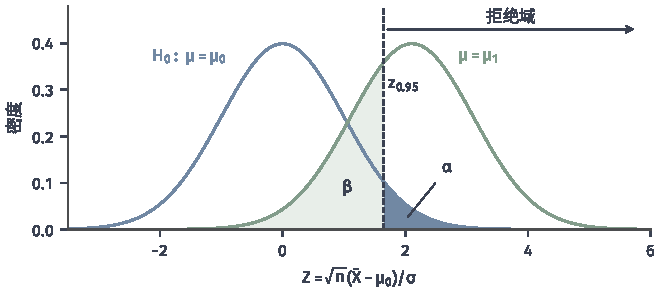
\includegraphics[width=112mm]{figures/01-basic-mathematics/05-probability-and-statistics-basics/matplotlib/pred-error-types/figure.pdf}
  \caption{单侧$z$检验的两类错误。蓝线是$H_0:\mu=\mu_0$下统计量$Z$的分布$\mathcal N(0,1)$，绿线是备择$\mu=\mu_1$下的分布$\mathcal N(\sqrt n(\mu_1-\mu_0)/\sigma,1)$，图中取$n=10$、$(\mu_1-\mu_0)/\sigma=2/3$，平移量约$2.11$。虚线为临界值$z_{0.95}\approx1.645$，其右侧为拒绝域。深蓝区域面积为$\alpha=0.05$（第一类错误），浅绿区域面积$\beta\approx0.32$（在$\mu_1$处的第二类错误），功效为$1-\beta\approx0.68$。}
  \label{fig:pred-error-types}
\end{figure}

\paragraph{影响功效的因素}

为了看清功效由什么决定，考虑正态总体、$\sigma$已知时的单侧问题$H_0:\mu\leq\mu_0$，$H_1:\mu>\mu_0$。检验统计量为$Z=\sqrt n(\bar X-\mu_0)/\sigma$，拒绝域为$Z>z_{1-\alpha}$。参数为$\mu$时，$\sqrt n(\bar X-\mu)/\sigma\sim\mathcal N(0,1)$，而
\[
 Z=\frac{\sqrt n(\bar X-\mu)}{\sigma}+\frac{\sqrt n(\mu-\mu_0)}{\sigma},
\]
所以
\begin{equation}
 \gamma(\mu)=\mathbb P_\mu(Z>z_{1-\alpha})
 =1-\Phi\bigl(z_{1-\alpha}-\sqrt n\,d\bigr)
 =\Phi\bigl(\sqrt n\,d-z_{1-\alpha}\bigr),
 \label{eq:pred-z-power}
\end{equation}
其中$d=(\mu-\mu_0)/\sigma$。
$\gamma(\mu)$随$\mu$增加，在$\Theta_0$的边界$\mu=\mu_0$处恰为$\alpha$，所以整个$\Theta_0$上的最大拒绝概率也是$\alpha$，检验的水平确为$\alpha$。

式~\eqref{eq:pred-z-power}表明功效只通过$\sqrt n\,d$依赖于问题。$d$是以总体标准差为单位度量的效应，称为\term{效应大小}（effect size）：真实偏离$\mu-\mu_0$越大、噪声$\sigma$越小，$d$越大；样本量则以$\sqrt n$的速度放大效应。图~\ref{fig:pred-power-curves}画出了不同样本量下的功效曲线：所有曲线在$d=0$处都经过$\alpha$，样本量越大，曲线越陡。

\begin{figure}[htbp]
  \centering
  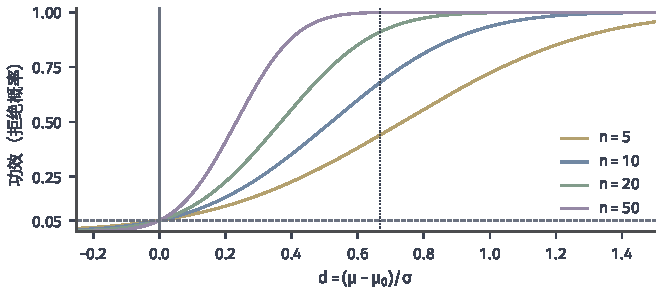
\includegraphics[width=112mm]{figures/01-basic-mathematics/05-probability-and-statistics-basics/matplotlib/pred-power-curves/figure.pdf}
  \caption{$\alpha=0.05$的单侧$z$检验的功效$\Phi(\sqrt n\,d-z_{0.95})$随效应大小$d=(\mu-\mu_0)/\sigma$变化，四条曲线对应$n=5,10,20,50$。$d=0$时所有曲线都等于虚线标出的$\alpha$；$d<0$属于原假设，拒绝概率低于$\alpha$。点线标出$d=2/3$，此处$n=10$的功效约$0.68$，$n=20$约$0.91$。}
  \label{fig:pred-power-curves}
\end{figure}

\begin{example}[功效与样本量]
\label{ex:pred-power-sample-size}
沿用$\sigma=1.5$，检验$H_0:\mu\leq500$，$\alpha=0.05$。若真均值为$501$，则$d=1/1.5\approx0.667$。$n=10$时功效为$\Phi(\sqrt{10}\times0.667-1.645)=\Phi(0.463)\approx0.68$，即约有$32\%$的机会漏掉这$1$ mL的多装。若要求功效达到$0.9$，需要$\sqrt n\,d-z_{0.95}\geq z_{0.9}$，即
\[
 n\geq\Bigl(\frac{z_{0.95}+z_{0.9}}{d}\Bigr)^2=\Bigl(\frac{1.645+1.282}{0.667}\Bigr)^2\approx19.3,
\]
至少需要$20$瓶。这种计算应当在收集数据之前完成。
\end{example}

\paragraph{显著性水平不是结论出错的概率}

$\alpha$是在$H_0$为真的条件下错误拒绝的概率，即$\mathbb P(\text{拒绝}\mid H_0\text{为真})$。人们常常想知道的却是反过来的条件概率：已经拒绝了，$H_0$其实为真的概率是多少？两者一般不相等，后者还取决于被检验的假设中有多少本来就为真。

\begin{example}[拒绝中有多少是错的]
\label{ex:pred-false-rejections}
设某实验室一年做$1000$次检验，其中$900$次$H_0$实际为真，$100$次$H_1$为真；每次检验的水平为$0.05$，在真实效应处的功效为$0.8$。$H_0$为真的$900$次中，约$900\times0.05=45$次被错误拒绝；$H_1$为真的$100$次中，约$80$次被正确拒绝。共拒绝约$125$次，其中$H_0$为真的占$45/125=36\%$，远高于$5\%$。如果真实效应更少或功效更低，这一比例还会更高。
\end{example}

\subsection{$p$值}

\paragraph{定义与计算}

拒绝域给出的是“拒绝”或“不拒绝”二选一的结论，没有说明证据有多强。例~\ref{ex:pred-filling-two-sided}中$t\approx4.19$远超临界值$2.262$，若观测值是$2.3$，结论同样是拒绝，但两者的说服力显然不同。$p$值把“观测结果有多极端”换算为原假设下的尾概率。

\begin{definition}[$p$值]
\label{def:pred-p-value}
设检验统计量$T$的取值越大，越不利于$H_0$。对观测值$t_{\mathrm{obs}}=T(\bm x)$，
\[
 p(\bm x)=\sup_{\theta\in\Theta_0}\mathbb P_\theta\bigl(T(\bm X)\geq t_{\mathrm{obs}}\bigr)
\]
称为\term{$p$值}（$p$-value），即在$H_0$下得到至少与观测结果同样极端的统计量的最大概率。
\end{definition}

定义先要求确定“极端”的顺序，这由$H_1$决定：右侧检验以$T$大为极端；左侧检验可改用$-T$；双侧检验以$|T|$大为极端。$H_0$是简单假设时，上确界就是该点处的尾概率；$H_0$是复合假设时，通常在$\Theta_0$的边界上取到，例如$H_0:\mu\leq500$时取$\mu=500$。

$p$值与拒绝域给出相同的结论：在水平$\alpha$下，$p(\bm x)\leq\alpha$时拒绝$H_0$。以简单原假设、$T$为连续型的情形说明：拒绝域取$R=\{T\geq c\}$，$c$满足$\mathbb P_{\theta_0}(T\geq c)=\alpha$。尾概率$\mathbb P_{\theta_0}(T\geq t)$随$t$递减，所以$t_{\mathrm{obs}}\geq c$当且仅当$\mathbb P_{\theta_0}(T\geq t_{\mathrm{obs}})\leq\alpha$，即$p\leq\alpha$。因此报告$p$值相当于同时报告了所有水平下的结论：$p$值是能够拒绝$H_0$的最小显著性水平。

在同样的条件下还有一个有用的事实：$H_0$为真时，$p$值服从$\operatorname U(0,1)$。记$G(t)=\mathbb P_{\theta_0}(T\geq t)$，则$p=G(T)$；对$0<u<1$，取$c_u$使$G(c_u)=u$，有$\mathbb P_{\theta_0}(G(T)\leq u)=\mathbb P_{\theta_0}(T\geq c_u)=u$。这说明规则“$p\leq\alpha$时拒绝”的第一类错误概率恰为$\alpha$。

\begin{example}[两台灌装机的$p$值]
\label{ex:pred-p-values}
对灌装机A（例~\ref{ex:pred-filling-two-sided}），双侧检验$H_0:\mu=500$的$p$值为
\[
 p=\mathbb P(|T_9|\geq4.19)=2\,\mathbb P(T_9\geq4.19)\approx0.0023,
\]
其中$T_9\sim t_9$。数据与原假设很不相容。

再从灌装机B抽取$8$瓶，灌装量（教学数据）为
\[
 500.2,\ 498.1,\ 501.9,\ 497.6,\ 499.4,\ 502.3,\ 498.8,\ 499.7.
\]
算得$\bar y=499.75$，$s_B\approx1.678$，$t=(499.75-500)/(1.678/\sqrt8)\approx-0.42$。双侧$p$值为$\mathbb P(|T_7|\geq0.42)\approx0.69$，即图~\ref{fig:pred-p-value-tail}中阴影的总面积。在$H_0$下，比这更极端的结果相当常见，数据没有提供否定$H_0$的证据。
\end{example}

\begin{figure}[htbp]
  \centering
  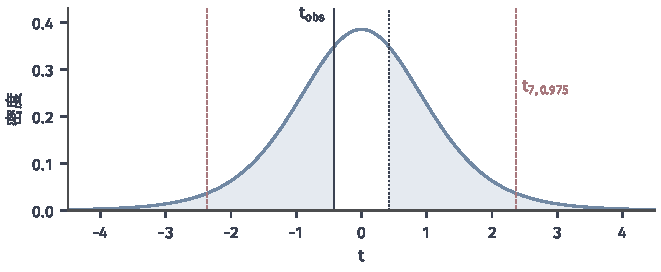
\includegraphics[width=112mm]{figures/01-basic-mathematics/05-probability-and-statistics-basics/matplotlib/pred-p-value-tail/figure.pdf}
  \caption{双侧$p$值是原假设分布的两侧尾面积。曲线为$t_7$分布的密度；实线标出灌装机B的观测值$t_{\mathrm{obs}}\approx-0.42$，点线是它关于零的对称点，两侧阴影面积之和约$0.69$即$p$值。红色虚线是$5\%$水平双侧检验的临界值$\pm t_{7,0.975}\approx\pm2.365$：观测值落在它们之间，相应地$p>0.05$。}
  \label{fig:pred-p-value-tail}
\end{figure}

\paragraph{常见误读}

$p$值是在$H_0$成立的条件下计算出来的，它不是“$H_0$为真的概率”。灌装机A的$p\approx0.0023$不意味着平均灌装量等于$500$的概率是$0.23\%$；后者需要给假设指定先验概率，属于上一节可信区间那一类问题。例~\ref{ex:pred-false-rejections}已经说明，即使$p$值很小，被拒绝的$H_0$中仍可能有相当比例本来为真。

不拒绝$H_0$也不等于证明了$H_0$。灌装机B的$p\approx0.69$只说明数据与$\mu=500$相容；它的$95\%$置信区间是$499.75\pm2.365\times0.593=[498.35,\,501.15]$，与之相容的还有$499$、$501$等许多数值。样本量小、功效低时，即使$H_0$不成立，也很可能不被拒绝。

$p$值的大小也不衡量效应的大小。灌装机A的偏离$\bar x-500=1.5$ mL，约为标称量的$0.3\%$；这一偏离是否重要，取决于成本与规范，而不是$p$值。反过来，若样本量极大，标准误趋于零，再微小的偏离也会给出极小的$p$值。所以报告检验结果时，应当同时报告估计值和置信区间：前者说明效应多大，后者说明估计有多精确。

\subsection{单总体均值检验}

\paragraph{统计量的选择}

前面的例子已经用过均值检验。系统地说，检验$\mu=\mu_0$所用的统计量与第~\ref{sec:pred-intervals}节的区间完全平行，按总体条件分三种情形：
\begin{center}
\begin{tabular}{lll}
  \toprule
  总体条件 & 统计量 & $H_0$下的分布\\
  \midrule
  正态，$\sigma$已知 & $Z=\dfrac{\bar X-\mu_0}{\sigma/\sqrt n}$ & $\mathcal N(0,1)$，精确\\[1.2ex]
  正态，$\sigma$未知 & $T=\dfrac{\bar X-\mu_0}{S/\sqrt n}$ & $t_{n-1}$，精确\\[1.2ex]
  独立同分布，方差有限 & $T=\dfrac{\bar X-\mu_0}{S/\sqrt n}$ & 近似$\mathcal N(0,1)$，$n$大时\\
  \bottomrule
\end{tabular}
\end{center}
第二种称为单样本\term{$t$检验}（$t$ test）。第三种情形的水平只在渐近意义下成立，例~\ref{ex:pred-exponential-coverage}中偏斜总体的覆盖不足，同样会表现为单侧检验的实际水平偏离名义值。

\paragraph{单侧与双侧拒绝域}

统计量确定之后，拒绝域的位置由备择假设决定。我们用灌装机A的数据，把同一个统计量放进三种检验问题中比较。

\begin{example}[灌装量的三种检验]
\label{ex:pred-filling-three-tests}
对例~\ref{ex:pred-filling-data}，$t\approx4.19$，自由度$9$，$\alpha=0.05$：
\begin{itemize}
  \item $H_1:\mu\neq500$：拒绝域$|t|>2.262$，$p=2\,\mathbb P(T_9\geq4.19)\approx0.0023$，拒绝；
  \item $H_1:\mu>500$：拒绝域$t>t_{9,0.95}=1.833$，$p=\mathbb P(T_9\geq4.19)\approx0.0012$，拒绝；
  \item $H_1:\mu<500$：拒绝域$t<-1.833$，$p=\mathbb P(T_9\leq4.19)\approx0.9988$，不拒绝。
\end{itemize}
同侧的单侧检验的临界值比双侧小，$p$值是双侧的一半，因为全部$\alpha$都放在了一侧。但这只在方向事先确定时才合理；看到$\bar x>500$之后再选择右侧检验，相当于把双侧检验的$p$值减半，实际水平会翻倍。
\end{example}

检验结论应与估计一起解释。这批数据的结论是：平均灌装量显著高于$500$ mL（$p\approx0.002$），估计多装$1.5$ mL，$95\%$置信区间为$[0.69,\,2.31]$ mL。以样本标准差为单位，偏离约为$1.5/1.13\approx1.3$个标准差，相对于瓶间波动并不算小；但相对于$500$ mL的总量只占约$0.3\%$。是否需要调整设备，取决于多装的成本与质量规范。

\subsection{两总体均值比较}

\paragraph{独立两组与配对数据}

比较两个总体的均值时，首先要看数据是怎样收集的。若两组观测分别来自不同的个体，例如从灌装机A、B各自抽瓶，两组相互独立，称为独立样本；若每个个体被测量两次，例如同一件样品分别用新旧两种方法测量，两次测量成对出现，称为配对数据。配对数据中，同一样品的两次测量共享样品自身的特性，因而相关；把它们当作两个独立组来分析，会把样品之间的差异混入比较。

配对数据的处理很简单：对每一对取差值$D_i=V_i-U_i$，问题就变为差值总体的均值$\mu_D$是否为零，即单总体均值检验。假设$D_1,\dots,D_n$独立同分布于正态总体，统计量$T=\bar D/(S_D/\sqrt n)$在$H_0:\mu_D=0$下服从$t_{n-1}$，这称为配对$t$检验。

\begin{example}[配对设计与错误的独立分析]
\label{ex:pred-paired}
$8$件样品分别用旧方法$u_i$与新方法$v_i$测量某成分含量（单位：mg，教学数据）：
\begin{center}
\begin{tabular}{lcccccccc}
  \toprule
  样品 & 1 & 2 & 3 & 4 & 5 & 6 & 7 & 8\\
  \midrule
  旧方法$u_i$ & 12.4 & 15.1 & 9.8 & 14.2 & 11.6 & 13.0 & 10.5 & 12.9\\
  新方法$v_i$ & 12.9 & 15.3 & 10.6 & 14.5 & 11.8 & 13.7 & 10.8 & 13.4\\
  差值$d_i$ & 0.5 & 0.2 & 0.8 & 0.3 & 0.2 & 0.7 & 0.3 & 0.5\\
  \bottomrule
\end{tabular}
\end{center}
差值的均值$\bar d=3.5/8=0.4375$，标准差$s_D\approx0.226$，于是$t=0.4375/(0.226/\sqrt8)\approx5.47$，自由度$7$，双侧$p\approx0.0009$；$\mu_D$的$95\%$置信区间为$0.4375\pm2.365\times0.080=[0.25,\,0.63]$。新方法系统地偏高约$0.44$ mg。

若错误地把两列当作独立样本，用下文的合并方差$t$检验，得到$p\approx0.62$，看不出任何差异。原因在于样品之间含量差异很大（从约$10$到约$15$ mg），独立分析把这部分差异算作噪声；取差值后，同一样品的特性相互抵消，只剩下方法差异和测量误差。
\end{example}

\paragraph{合并方差$t$检验}

再来看独立样本。设$X_1,\dots,X_{n_1}$独立同分布于$\mathcal N(\mu_1,\sigma^2)$，$Y_1,\dots,Y_{n_2}$独立同分布于$\mathcal N(\mu_2,\sigma^2)$，两组相互独立。这里的关键假设是\emph{两总体方差相等}。检验$H_0:\mu_1=\mu_2$。

我们仿照单样本情形构造枢轴量。由独立性，$\bar X-\bar Y\sim\mathcal N\bigl(\mu_1-\mu_2,\ \sigma^2(1/n_1+1/n_2)\bigr)$。两组的样本方差都估计同一个$\sigma^2$，把它们按自由度加权合并：
\[
 S_p^2=\frac{(n_1-1)S_X^2+(n_2-1)S_Y^2}{n_1+n_2-2}.
\]
由第~\ref{sec:samp-chi-square}节，$(n_1-1)S_X^2/\sigma^2\sim\chi^2_{n_1-1}$，$(n_2-1)S_Y^2/\sigma^2\sim\chi^2_{n_2-1}$，二者独立。卡方变量是独立标准正态变量的平方和，两个独立卡方变量相加，相当于把两组独立标准正态变量合在一起求平方和，所以$(n_1+n_2-2)S_p^2/\sigma^2\sim\chi^2_{n_1+n_2-2}$。它又与$\bar X-\bar Y$独立，因为每组内样本均值与样本方差独立，两组之间也独立。按$t$分布的定义（第~\ref{sec:samp-t}节），
\begin{equation}
 T=\frac{(\bar X-\bar Y)-(\mu_1-\mu_2)}{S_p\sqrt{1/n_1+1/n_2}}\sim t_{n_1+n_2-2}.
 \label{eq:pred-pooled-t}
\end{equation}
令$\mu_1-\mu_2=0$即得检验统计量，称为合并方差$t$检验；反解$T$也得到$\mu_1-\mu_2$的置信区间。

\begin{example}[两台灌装机的比较]
\label{ex:pred-two-machines}
灌装机A（例~\ref{ex:pred-filling-data}）：$n_1=10$，$\bar x=501.5$，$s_X^2\approx1.282$；灌装机B（例~\ref{ex:pred-p-values}）：$n_2=8$，$\bar y=499.75$，$s_Y^2\approx2.814$。合并方差
\[
 s_p^2=\frac{9\times1.282+7\times2.814}{16}=\frac{11.54+19.70}{16}\approx1.953,
\]
标准误$s_p\sqrt{1/10+1/8}\approx0.663$，$t=1.75/0.663\approx2.64$，自由度$16$，双侧$p\approx0.018$。$\mu_1-\mu_2$的$95\%$置信区间为$1.75\pm2.120\times0.663=[0.34,\,3.16]$。
\end{example}

\paragraph{Welch方法}

等方差是一个实质性的假设。上例中两组样本方差相差一倍以上，等方差未必成立。若两总体方差不等而样本量又不同，合并方差会把两组的波动按错误的权重混合，$T$的实际分布偏离$t_{n_1+n_2-2}$，检验水平可能明显失真。

不假设等方差时，自然的做法是分别估计两组的方差：
\[
 T_W=\frac{\bar X-\bar Y}{\sqrt{S_X^2/n_1+S_Y^2/n_2}}.
\]
这时$T_W$在$H_0$下不再精确服从任何$t$分布，但可以用一个$t$分布近似，其自由度由Welch--Satterthwaite公式给出：
\[
 \nu=\frac{\bigl(S_X^2/n_1+S_Y^2/n_2\bigr)^2}{\dfrac{(S_X^2/n_1)^2}{n_1-1}+\dfrac{(S_Y^2/n_2)^2}{n_2-1}}.
\]
这个公式的想法是：选择$\nu$，使$\nu\cdot(S_X^2/n_1+S_Y^2/n_2)/(\sigma_1^2/n_1+\sigma_2^2/n_2)$的前两阶矩与$\chi^2_\nu$相同，再把未知方差换成样本方差。所得的\term{Welch检验}（Welch test）是近似方法，但在两总体方差相等与否时都表现良好，因此当没有充分理由相信等方差时，通常默认使用它。

\begin{example}[两台灌装机的Welch检验]
\label{ex:pred-welch}
续例~\ref{ex:pred-two-machines}，$s_X^2/n_1\approx0.128$，$s_Y^2/n_2\approx0.352$，标准误$\sqrt{0.128+0.352}\approx0.693$，$t_W=1.75/0.693\approx2.53$，自由度$\nu\approx11.8$，双侧$p\approx0.027$。结论与合并方差检验相同，但标准误略大、自由度更小，证据显得稍弱。
\end{example}

\subsection{比例检验}

\paragraph{精确二项检验}

合同规定封口不合格率不得超过$5\%$。抽查$40$瓶发现$6$瓶不合格（例~\ref{ex:pred-wald}），能否认定不合格率超标？检验问题为$H_0:p\leq0.05$，$H_1:p>0.05$。

不合格数$S\sim\operatorname{Bin}(40,p)$，$S$越大越不利于$H_0$，拒绝域取右尾$\{S\geq c\}$。按第~\ref{sec:pred-intervals}节证明的单调性，$\mathbb P_p(S\geq c)$随$p$增加，因此$\Theta_0=[0,0.05]$上的最大拒绝概率在边界$p=0.05$处取到，只需在$\operatorname{Bin}(40,0.05)$下计算。$H_0$下的尾概率为
\[
 \mathbb P(S\geq4)\approx0.138,\qquad\mathbb P(S\geq5)\approx0.048,\qquad\mathbb P(S\geq6)\approx0.014.
\]
要使水平不超过$0.05$，最小的临界值是$c=5$，拒绝域为$\{S\geq5\}$，实际水平为$0.048$。观测值$s=6$落入拒绝域，$p$值为$\mathbb P(S\geq6)\approx0.014$，拒绝$H_0$。

这里实际水平$0.048$略低于名义值$0.05$，这又是离散性的结果：$S$只取整数，尾概率只能取有限个值，一般无法恰好等于$\alpha$。若取$c=4$，水平升至$0.138$，超出要求。所以精确二项检验通常是保守的，这与Clopper--Pearson区间的保守覆盖出自同一原因。

双侧问题$H_0:p=p_0$还需决定怎样合并两侧尾部。常用做法是计算观测值所在一侧的尾概率并乘以$2$（不超过$1$）；由于二项分布在$p_0\neq1/2$时不对称，不同的合并方式可能给出不同的$p$值，报告时应说明所用方法。

\paragraph{正态近似}

样本量较大时，可以用正态分布近似$S$。$H_0:p=p_0$下$\hat p$的均值为$p_0$、方差为$p_0(1-p_0)/n$，统计量
\[
 Z=\frac{\hat p-p_0}{\sqrt{p_0(1-p_0)/n}}
\]
近似服从$\mathcal N(0,1)$。注意分母使用的是原假设下的$p_0$，而不是$\hat p$：检验在$H_0$成立的前提下计算统计量的分布，方差应按$H_0$来算。

\begin{example}[精确计算与正态近似的比较]
\label{ex:pred-binomial-approx}
对$n=40$、$s=6$、$p_0=0.05$，$\hat p=0.15$，$Z=(0.15-0.05)/\sqrt{0.05\times0.95/40}\approx2.90$，近似$p$值为$1-\Phi(2.90)\approx0.0019$，只有精确值$0.014$的约七分之一。图~\ref{fig:pred-binomial-test}说明了原因：$np_0=2$，二项分布明显右偏，正态曲线的右尾下降得比真实概率快得多。这里结论碰巧相同。若观测值是$s=5$，精确$p$值为$0.048$，刚好在$5\%$水平下拒绝；近似$p$值约为$0.015$，又一次把证据夸大了约三倍。在更接近临界的情形中，这种夸大足以改变结论。
\end{example}

\begin{figure}[htbp]
  \centering
  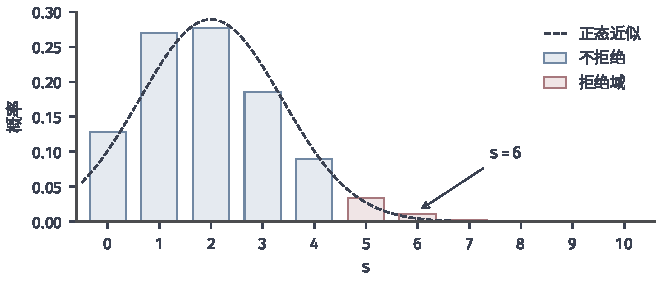
\includegraphics[width=112mm]{figures/01-basic-mathematics/05-probability-and-statistics-basics/matplotlib/pred-binomial-test/figure.pdf}
  \caption{原假设$p=0.05$下不合格数$S\sim\operatorname{Bin}(40,0.05)$的概率。红色柱为$5\%$水平的拒绝域$\{S\geq5\}$，总概率约$0.048$；箭头标出观测值$s=6$，其右尾概率约$0.014$即精确$p$值。虚线是均值$2$、方差$1.9$的正态近似密度，它在右尾明显低于二项概率，因而低估了$p$值。}
  \label{fig:pred-binomial-test}
\end{figure}

一个常用的经验规则是：$np_0$与$n(1-p_0)$都至少约为$10$时，正态近似才比较可靠。这是经验判断，不是定理；可以计算精确值时，应优先使用精确的二项检验。

\subsection{方差检验}

\paragraph{单个正态总体}

设备规范要求灌装量的标准差不超过$1.5$ mL。对正态样本，检验$H_0:\sigma^2=\sigma_0^2$用第~\ref{sec:pred-intervals}节的卡方枢轴量，在$H_0$下
\[
 \chi^2=\frac{(n-1)S^2}{\sigma_0^2}\sim\chi^2_{n-1}.
\]
双侧检验的拒绝域为$\{\chi^2<\chi^2_{n-1,\alpha/2}\}\cup\{\chi^2>\chi^2_{n-1,1-\alpha/2}\}$；关心方差是否过大时，用右侧拒绝域$\{\chi^2>\chi^2_{n-1,1-\alpha}\}$。

\begin{example}[灌装量的方差检验]
\label{ex:pred-variance-test}
对例~\ref{ex:pred-filling-data}检验$H_0:\sigma=1.5$，$\chi^2=11.54/2.25\approx5.13$。双侧$5\%$水平的拒绝域是$\chi^2<2.700$或$\chi^2>19.023$，观测值不在其中，双侧$p\approx0.35$。若只关心波动是否过大，$H_1:\sigma>1.5$，则观测值在分布的左侧，更没有理由拒绝。这与例~\ref{ex:pred-filling-variance-interval}中$\sigma$的区间$[0.779,\,2.067]$包含$1.5$是一致的。
\end{example}

和方差区间一样，这个检验的水平完全依赖正态性；总体尾部较厚时，检验会过多地拒绝，并且不因样本量增大而改善。

\paragraph{两个正态总体的$F$检验}

比较两台灌装机的波动，检验$H_0:\sigma_1^2=\sigma_2^2$。设两组独立，各自来自正态总体。$(n_1-1)S_X^2/\sigma_1^2$与$(n_2-1)S_Y^2/\sigma_2^2$分别服从$\chi^2_{n_1-1}$、$\chi^2_{n_2-1}$且相互独立，按第~\ref{sec:samp-f}节$F$分布的定义，
\[
 \frac{S_Y^2/\sigma_2^2}{S_X^2/\sigma_1^2}\sim F_{n_2-1,\,n_1-1}.
\]
$H_0$下$\sigma_1^2=\sigma_2^2$相消，统计量$F=S_Y^2/S_X^2\sim F_{n_2-1,n_1-1}$，比值过大或过小都不利于$H_0$。

\begin{example}[两台灌装机的方差比较]
\label{ex:pred-f-test}
续例~\ref{ex:pred-two-machines}，$F=2.814/1.282\approx2.19$，自由度$(7,9)$。$F_{7,9,0.025}\approx0.207$，$F_{7,9,0.975}\approx4.197$，观测值落在两者之间，双侧$p\approx0.27$，不拒绝等方差假设。
\end{example}

这个结果不能读作“两台机器的方差相等”。两组各只有十个左右的观测，方差比的估计很粗糙，即使真实方差相差一倍，$F$检验也很可能不拒绝。正因如此，不宜先用$F$检验判断等方差、再据此在合并方差与Welch方法之间选择；直接使用Welch方法更稳妥。此外，$F$检验对非正态性同样敏感，原因与卡方检验相同。

\subsection{检验与置信区间的关系}

\paragraph{由检验族构造置信集合}

例~\ref{ex:pred-variance-test}中，检验不拒绝$\sigma=1.5$，而$\sigma$的置信区间恰好包含$1.5$，这不是巧合。对每一个可能的参数值$\theta_0$，都可以检验$H_0:\theta=\theta_0$；把所有未被拒绝的$\theta_0$收集起来，就得到一个置信集合。

\begin{theorem}[检验与置信集合的对偶]
\label{thm:pred-test-interval-duality}
设对每个$\theta_0\in\Theta$，都有$H_0:\theta=\theta_0$的水平为$\alpha$的检验，把它的拒绝域直接写成样本的集合$R(\theta_0)$，即$\mathbb P_{\theta_0}\bigl(\bm X\in R(\theta_0)\bigr)\leq\alpha$。令
\[
 C(\bm X)=\{\theta_0\in\Theta:\bm X\notin R(\theta_0)\},
\]
则对每个$\theta\in\Theta$，$\mathbb P_\theta\bigl(\theta\in C(\bm X)\bigr)\geq1-\alpha$。反过来，若$C(\bm X)$是置信水平为$1-\alpha$的置信集合（即把定义~\ref{def:pred-confidence-interval}中的区间换成一般的参数集合），则“$\theta_0\notin C(\bm X)$时拒绝”是$H_0:\theta=\theta_0$的水平为$\alpha$的检验。
\end{theorem}

\begin{proof}
由$C$的定义，$\theta\in C(\bm X)$当且仅当$\bm X\notin R(\theta)$。故$\mathbb P_\theta\bigl(\theta\in C(\bm X)\bigr)=1-\mathbb P_\theta\bigl(\bm X\in R(\theta)\bigr)\geq1-\alpha$。反方向，拒绝域为$\{\bm X:\theta_0\notin C(\bm X)\}$，其在$\theta_0$下的概率为$1-\mathbb P_{\theta_0}\bigl(\theta_0\in C(\bm X)\bigr)\leq\alpha$。
\end{proof}

定理说明，“检验”和“置信集合”是同一族事件$\{\bm X\notin R(\theta_0)\}$的两种读法：固定$\theta_0$看哪些样本会拒绝它，得到检验；固定样本看哪些$\theta_0$未被拒绝，得到置信集合。定理给出的置信集合不一定是区间，但在常见的单参数问题中通常是。

\paragraph{均值双侧检验的对应}

以$t$检验为例。水平$\alpha$的双侧$t$检验在$|\bar x-\mu_0|/(s/\sqrt n)\leq t_{n-1,1-\alpha/2}$时不拒绝$H_0:\mu=\mu_0$，这个不等式对$\mu_0$解出来就是
\[
 \bar x-t_{n-1,1-\alpha/2}\frac s{\sqrt n}\leq\mu_0\leq\bar x+t_{n-1,1-\alpha/2}\frac s{\sqrt n},
\]
恰好是$t$区间~\eqref{eq:pred-t-interval}。所以对灌装机A，$500$不在$95\%$区间$[500.69,\,502.31]$中，等价于$5\%$水平的双侧$t$检验拒绝$\mu=500$。图~\ref{fig:pred-test-interval-duality}把双侧$p$值看作$\mu_0$的函数：曲线在$\bar x$处达到$1$，向两侧下降；$p$值高于$0.05$的$\mu_0$恰好组成$95\%$置信区间。

\begin{figure}[htbp]
  \centering
  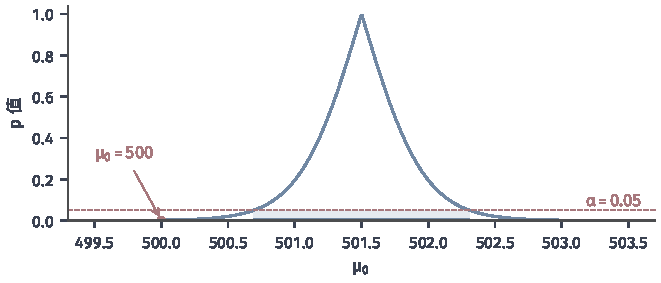
\includegraphics[width=112mm]{figures/01-basic-mathematics/05-probability-and-statistics-basics/matplotlib/pred-test-interval-duality/figure.pdf}
  \caption{灌装机A数据的双侧$t$检验$p$值作为待检验值$\mu_0$的函数，$p(\mu_0)=2\,\mathbb P\bigl(T_9\geq|\bar x-\mu_0|/(s/\sqrt{10})\bigr)$。红色虚线为$\alpha=0.05$；曲线在虚线之上的$\mu_0$不被拒绝，它们构成横轴上加粗标出的$95\%$置信区间$[500.69,\,502.31]$。红点为$\mu_0=500$，$p\approx0.0023$，位于区间外。}
  \label{fig:pred-test-interval-duality}
\end{figure}

这种对应要求区间与检验由同一族构造得到：相同的统计量、相同的标准误、相同的尾部规则。若两者不匹配，就不能直接用区间判断检验结果。

\begin{example}[不匹配的区间与检验]
\label{ex:pred-mismatch}
单侧检验对应单侧置信界，而不是双侧区间。灌装机A的右侧检验$H_1:\mu>500$对应置信下界$\bar x-t_{9,0.95}\,s/\sqrt{10}\approx500.84$：$500$低于它，故拒绝。若改用双侧$95\%$区间判断单侧检验，实际相当于在$2.5\%$水平下检验。

比例问题中的不匹配更明显。对$n=40$、$s=6$，Wald区间$[0.039,\,0.261]$包含$0.05$；但例~\ref{ex:pred-binomial-approx}中的正态近似检验给出$Z\approx2.90$，强烈拒绝$p=0.05$。两者的标准误不同：Wald区间用$\sqrt{\hat p(1-\hat p)/n}\approx0.056$，检验用$\sqrt{p_0(1-p_0)/n}\approx0.034$。由这个检验族反解得到的区间，即把$|\hat p-p_0|\leq z_{0.975}\sqrt{p_0(1-p_0)/n}$对$p_0$解出的二次不等式的解集，约为$[0.071,\,0.291]$，它不包含$0.05$，与检验结论一致。
\end{example}

\section{未来观测的预测}
\label{sec:pred-prediction}

前两节的对象都是参数，它是总体的一个固定特征。质检员还关心另一类问题：下一瓶会装多少？这时要猜测的是一个尚未发生的随机结果，即使参数完全已知，也不可能准确猜中。本节先明确预测的对象和点预测的标准，再分析预测误差的来源，然后在正态模型中构造预测区间，最后用后验分布给出另一种预测方式。

\subsection{预测对象与点预测}

\paragraph{三种不同的对象}

在灌装的例子里，至少有三种量都可以称为“估计灌装量”：总体均值$\mu$，这是参数；下一瓶的灌装量$X_{n+1}$，这是单个未来观测；下一批$m$瓶的平均灌装量$\bar X'_m$，这是未来观测的汇总量。三者都可以用同一个数$\bar x=501.5$去猜，但猜测的误差完全不同。

设未来观测与已有样本独立同分布，方差为$\sigma^2$。参数$\mu$固定不动，误差只来自估计；$X_{n+1}$本身围绕$\mu$以方差$\sigma^2$波动；$\bar X'_m$的方差为$\sigma^2/m$，介于二者之间。$m=1$时它就是单个观测，$m\to\infty$时它趋于参数。所以说明“预测什么”是第一步：对象改变后，误差的含义和大小都随之改变。

\paragraph{平方误差下的最优点预测}

先只用一个数来预测随机变量$Y$。若用常数$c$，并以平方误差$(Y-c)^2$衡量损失，设$\mathbb E Y^2<\infty$，则
\begin{equation}
 \mathbb E(Y-c)^2=\mathbb E\bigl((Y-\mathbb EY)+(\mathbb EY-c)\bigr)^2=\operatorname{Var}(Y)+(\mathbb EY-c)^2,
 \label{eq:pred-mse-constant}
\end{equation}
交叉项$2(\mathbb EY-c)\,\mathbb E(Y-\mathbb EY)=0$。右边第一项与$c$无关，第二项在$c=\mathbb EY$时为零，所以均值是平方误差下的最优常数预测，最小误差就是方差。

若预测时还能观测到另一个变量$X$，预测可以写成$X$的函数$g(X)$。第~\ref{sec:rvec-conditional-expectation}节的条件期望$r(X)=\mathbb E(Y\mid X)$满足：对任何$X$的函数$h(X)$（使下式中的期望有限），$\mathbb E\bigl[(Y-r(X))h(X)\bigr]=0$。这可以由塔性质$\mathbb E\bigl[\mathbb E(Y\mid X)h(X)\bigr]=\mathbb E[Yh(X)]$得到。取$h=r-g$，与式~\eqref{eq:pred-mse-constant}同样展开，交叉项消失：
\begin{equation}
 \mathbb E\bigl(Y-g(X)\bigr)^2=\mathbb E\bigl(Y-r(X)\bigr)^2+\mathbb E\bigl(r(X)-g(X)\bigr)^2.
 \label{eq:pred-mse-conditional}
\end{equation}
因此在有限二阶矩条件下，条件均值$\mathbb E(Y\mid X)$是平方误差意义下的最优预测，第一项是任何预测都无法消除的误差。第~\ref{sec:pred-regression}节的回归函数$\beta_0+\beta_1x$正是一个条件均值的模型。

最优预测依赖于损失的选择。若改用绝对误差$|Y-c|$，最优常数是中位数而不是均值。

\begin{example}[均值与中位数作为预测]
\label{ex:pred-mean-median}
设某商品每日退货数$Y$取$0,1,10$，概率分别为$0.5,0.3,0.2$。$\mathbb EY=0.3+2=2.3$，平方误差下最优预测是$2.3$，最小均方误差为$\operatorname{Var}(Y)=\mathbb EY^2-2.3^2=20.3-5.29=15.01$。若按绝对误差，预测值$c\in[0,1]$时期望损失为$0.5c+0.3(1-c)+0.2(10-c)=2.3$，与$c$无关，区间$[0,1]$中的每个点都是中位数，也都是最优预测；而用$2.3$时期望绝对误差为$0.5\times2.3+0.3\times1.3+0.2\times7.7=3.08$。罕见的大值把均值拉高，中位数则不受影响。
\end{example}

\subsection{预测误差的来源}

\paragraph{参数已知时}

回到正态位置模型：$X_1,\dots,X_n,X_{n+1}$独立同分布于$\mathcal N(\mu,\sigma^2)$，要用前$n$个观测预测$X_{n+1}$。先设想$\mu$已知。由上一小节，最优点预测是$\mu$，预测误差$X_{n+1}-\mu\sim\mathcal N(0,\sigma^2)$。这部分误差来自新观测自身的随机波动，与历史数据的多少无关，称为不可约误差。即使知道总体的一切，也无法消除它。

\paragraph{参数需要估计时}

实际中$\mu$未知，只能用$\bar X$代替。预测误差变为
\[
 X_{n+1}-\bar X=(X_{n+1}-\mu)-(\bar X-\mu).
\]
第一项是新观测的波动，第二项是估计参数带来的误差。由于$X_{n+1}$与$X_1,\dots,X_n$独立，两项独立，方差相加：
\begin{equation}
 \mathbb E(X_{n+1}-\bar X)^2=\operatorname{Var}(X_{n+1}-\bar X)=\sigma^2+\frac{\sigma^2}n=\sigma^2\Bigl(1+\frac1n\Bigr).
 \label{eq:pred-prediction-variance}
\end{equation}
这里第一个等号用到$\mathbb E(X_{n+1}-\bar X)=0$。这个结论只需要独立同分布与有限方差，不需要正态性。

\begin{example}[两种误差的相对大小]
\label{ex:pred-error-sources}
取$\sigma=1.5$，$n=10$。新观测的波动贡献$\sigma^2=2.25$，参数估计贡献$\sigma^2/n=0.225$，总预测均方误差$2.475$，其中参数误差只占约$9\%$。把样本量增至$100$，参数误差降为$0.0225$，总误差$2.2725$，只减少了约$8\%$。增加历史数据很快就无法再改善单瓶的预测。
\end{example}

\subsection{正态位置模型的预测区间}

\paragraph{精确预测区间}

点预测之外，我们希望给出一个区间，使下一瓶的灌装量以指定概率落在其中。

\begin{definition}[预测区间]
\label{def:pred-prediction-interval}
设$L(\bm X)\leq U(\bm X)$是样本$\bm X=(X_1,\dots,X_n)$的统计量，$Y$是尚未观测的随机变量。若对模型中的每个参数，
\[
 \mathbb P\bigl(L(\bm X)\leq Y\leq U(\bm X)\bigr)\geq1-\alpha,
\]
则称$[L(\bm X),U(\bm X)]$为$Y$的水平为$1-\alpha$的\term{预测区间}（prediction interval）。这里的概率对样本$\bm X$与未来观测$Y$联合计算。
\end{definition}

与置信区间相比，被覆盖的对象从固定参数变成了随机变量，概率也同时包含了样本和新观测两部分随机性。

在正态位置模型中，由式~\eqref{eq:pred-prediction-variance}，$X_{n+1}-\bar X\sim\mathcal N\bigl(0,\sigma^2(1+1/n)\bigr)$，它是独立正态变量的线性组合，因而仍是正态的。为了处理未知的$\sigma$，再用$S$代替它。$X_{n+1}$与$(\bar X,S^2)$独立，因为后者只依赖$X_1,\dots,X_n$；又由第~\ref{sec:samp-normal}节，$\bar X$与$S^2$独立。所以$X_{n+1}$、$\bar X$、$S^2$三者相互独立，$X_{n+1}-\bar X$作为前两者的函数与$S^2$独立。按$t$分布的定义，
\[
 \frac{X_{n+1}-\bar X}{S\sqrt{1+1/n}}
 =\frac{(X_{n+1}-\bar X)\big/\bigl(\sigma\sqrt{1+1/n}\bigr)}{\sqrt{\dfrac{(n-1)S^2/\sigma^2}{n-1}}}
 \sim t_{n-1}.
\]
它的分布不含未知参数，反解得到$X_{n+1}$的预测区间
\begin{equation}
 \bar X\pm t_{n-1,1-\alpha/2}\,S\sqrt{1+\frac1n}.
 \label{eq:pred-normal-prediction-interval}
\end{equation}
对正态总体，其覆盖概率恰为$1-\alpha$。

\begin{example}[下一瓶的预测区间]
\label{ex:pred-filling-prediction}
对例~\ref{ex:pred-filling-data}，$95\%$预测区间为
\[
 501.5\pm2.262\times1.1324\times\sqrt{1.1}=501.5\pm2.687=[498.81,\,504.19].
\]
它比均值的$t$区间$[500.69,\,502.31]$宽约$3.3$倍。前者说的是下一瓶，后者说的是平均灌装量。
\end{example}

\paragraph{两种宽度的比较}

把预测区间~\eqref{eq:pred-normal-prediction-interval}与均值区间~\eqref{eq:pred-t-interval}放在一起看，两者的中心相同，分位数相同，只有半宽中的因子不同：均值区间是$1/\sqrt n$，预测区间是$\sqrt{1+1/n}$，比值为$\sqrt{n+1}$。$n\to\infty$时，$1/\sqrt n\to0$，均值区间收缩到一个点；$\sqrt{1+1/n}\to1$，预测区间趋于$\mu\pm z_{1-\alpha/2}\sigma$，这正是参数已知时新观测的波动范围。图~\ref{fig:pred-interval-widths}以$\sigma$已知的情形画出了这两条曲线：增加样本可以消除参数误差，但无法消除新观测的噪声。

\begin{figure}[htbp]
  \centering
  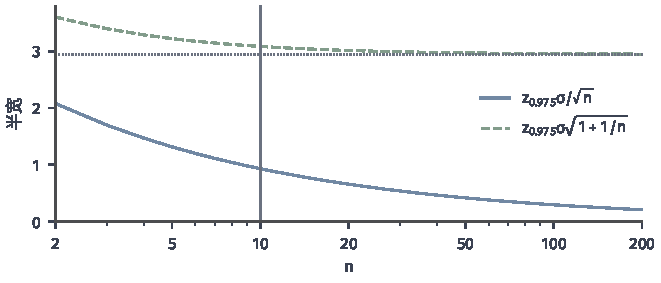
\includegraphics[width=112mm]{figures/01-basic-mathematics/05-probability-and-statistics-basics/matplotlib/pred-interval-widths/figure.pdf}
  \caption{$\sigma=1.5$已知时，$95\%$均值置信区间与预测区间的半宽随样本量$n$变化（横轴为对数刻度）。蓝实线$1.96\sigma/\sqrt n$趋于零；绿虚线$1.96\sigma\sqrt{1+1/n}$趋于点线标出的极限$1.96\sigma\approx2.94$。竖线标出$n=10$，此时两者分别约为$0.93$与$3.08$。}
  \label{fig:pred-interval-widths}
\end{figure}

预测区间对正态性的依赖比均值区间更强。均值区间在非正态总体下还有中心极限定理的大样本保证，因为$\bar X$是许多观测的平均；预测区间要覆盖的却是单个观测$X_{n+1}$，它的分布就是总体分布本身，不会因为$n$增大而变得接近正态。若总体偏斜或厚尾，式~\eqref{eq:pred-normal-prediction-interval}的覆盖率即使在大样本下也可能偏离名义值。这时可以改用基于样本分位数等不依赖分布形式的方法，相关内容见\BookChapterRef{chap:statistical-inference}{卷4《数学准备：流形、概率分布与统计推断》的“统计推断”章}。

\subsection{后验预测}

\paragraph{后验预测分布}

在贝叶斯框架中，参数的不确定性已由后验分布描述，预测可以直接由它推出。设给定参数$\theta$时，未来观测$Y$与已有样本$\bm X$条件独立，$Y$的密度（或质量函数）为$f(y\mid\theta)$。对后验分布求平均，
\begin{equation}
 f(y\mid\bm x)=\int_\Theta f(y\mid\theta)\,\pi(\theta\mid\bm x)\,\mathrm d\theta,
 \label{eq:pred-posterior-predictive}
\end{equation}
其中$\pi(\theta\mid\bm x)$是后验密度；参数离散时积分换成求和。这一分布称为\term{后验预测分布}（posterior predictive distribution）。它的推导就是全概率公式：$Y$与$\theta$在给定$\bm x$下的联合密度为$f(y\mid\theta,\bm x)\pi(\theta\mid\bm x)$，由条件独立性，$f(y\mid\theta,\bm x)=f(y\mid\theta)$，再对$\theta$积分即得边缘密度。

式~\eqref{eq:pred-posterior-predictive}中有两层不确定性：被积函数$f(y\mid\theta)$描述参数给定时新观测的波动，权重$\pi(\theta\mid\bm x)$描述参数本身的不确定性。这与前面分析的两种预测误差来源一一对应。与之相比，直接把点估计$\hat\theta$代入$f(y\mid\hat\theta)$的“代入预测”只保留了第一层，因而低估了预测的不确定性。

\paragraph{Beta--Bernoulli模型}

在Beta--Bernoulli模型中，下一瓶是否不合格$X_{n+1}\in\{0,1\}$，给定$p$时$\mathbb P(X_{n+1}=1\mid p)=p$。由式~\eqref{eq:pred-posterior-predictive}，
\[
 \mathbb P(X_{n+1}=1\mid\bm x)=\int_0^1p\,\pi(p\mid\bm x)\,\mathrm dp=\mathbb E(p\mid\bm x)=\frac{a+s}{a+b+n},
\]
最后一步用到$\operatorname{Beta}(a+s,b+n-s)$的均值。下一次成功的预测概率就是后验均值。

\begin{example}[下一瓶不合格的概率]
\label{ex:pred-beta-predictive}
续例~\ref{ex:pred-beta-credible}，均匀先验下，$40$瓶中$6$瓶不合格，下一瓶不合格的后验预测概率为$(1+6)/(2+40)=1/6\approx0.167$，略高于样本比例$0.15$。若$20$瓶全部合格，后验预测概率为$1/22\approx0.045$，而不是代入$\hat p=0$得到的$0$。均匀先验相当于事先多看了一次成功和一次失败，使预测不会因为尚未见过某种结果就断言它不可能发生。
\end{example}

\paragraph{高斯均值模型}

在例~\ref{ex:pred-normal-credible}的模型中，$\sigma^2$已知，$\mu$的后验为$\mathcal N(\mu_n,\tau_n^2)$。新观测可以写成$X_{n+1}=\mu+\varepsilon$，其中在给定数据下$\mu\sim\mathcal N(\mu_n,\tau_n^2)$，$\varepsilon\sim\mathcal N(0,\sigma^2)$，且二者独立。独立正态变量之和仍为正态，均值与方差分别相加，所以后验预测分布为
\begin{equation}
 X_{n+1}\mid\bm x\sim\mathcal N\bigl(\mu_n,\ \sigma^2+\tau_n^2\bigr).
 \label{eq:pred-normal-posterior-predictive}
\end{equation}
预测方差中$\sigma^2$是观测噪声，$\tau_n^2$是参数后验的方差。$n\to\infty$时$\tau_n^2\to0$，预测方差趋于$\sigma^2$，与频率学派预测区间的极限一致。

\begin{example}[下一瓶的后验预测区间]
\label{ex:pred-normal-predictive}
续例~\ref{ex:pred-normal-credible}，$\mu_n\approx501.22$，$\tau_n^2\approx0.184$，$\sigma^2=2.25$。预测方差$2.25+0.184=2.434$，标准差约$1.560$，$95\%$后验预测区间为$501.22\pm1.96\times1.560=[498.17,\,504.28]$。

图~\ref{fig:pred-posterior-predictive}比较了三条分布：后验分布集中在$501.2$附近，宽度由$\tau_n\approx0.43$决定；后验预测分布中心相同，但宽度约为$1.56$，主要由观测噪声决定。代入预测$\mathcal N(\mu_n,\sigma^2)$的标准差$1.5$只比$1.56$小一点，这是因为$10$个观测已经把参数确定得较好；样本很少时，二者的差别会大得多。
\end{example}

\begin{figure}[htbp]
  \centering
  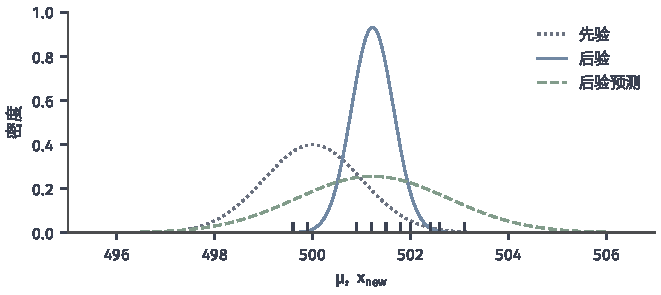
\includegraphics[width=112mm]{figures/01-basic-mathematics/05-probability-and-statistics-basics/matplotlib/pred-posterior-predictive/figure.pdf}
  \caption{灌装量的先验、后验与后验预测（$\sigma^2=2.25$已知）。灰色点线为先验$\mathcal N(500,1)$；蓝实线为观测$10$瓶后$\mu$的后验$\mathcal N(501.22,0.184)$；绿虚线为下一瓶灌装量的后验预测分布$\mathcal N(501.22,2.434)$。横轴下方的短竖线为$10$个观测值。后验描述平均灌装量的不确定性，后验预测描述单瓶灌装量的不确定性，后者宽得多。}
  \label{fig:pred-posterior-predictive}
\end{figure}

这个区间与例~\ref{ex:pred-filling-prediction}的$t$预测区间$[498.81,\,504.19]$长度相近，但依据不同：后验预测区间假定$\sigma$已知并使用了先验，概率是对给定数据下的$\mu$和$\varepsilon$计算的；$t$预测区间不需要先验，也不假定$\sigma$已知，概率是对样本和新观测的重复抽样计算的。

\section{简单线性回归中的统计推断}
\label{sec:pred-regression}

前三节的模型只有一个位置参数。许多问题关心的是两个变量之间的关系：广告投入增加时，销量平均增加多少？给定一笔预算，销量大致会是多少？本节在简单线性回归模型中回答这些问题。第~\ref{sec:ls-least-squares}节已经给出了最小二乘的计算方法，这里把它放进统计模型，依次完成估计、区间、检验与预测，并看到前三节的方法如何在同一个模型中各司其职。

全节使用下面的教学数据。

\begin{example}[广告投入与销量]
\label{ex:pred-ad-data}
某公司在$8$个城市的月广告投入$x_i$（万元）与当月销量$y_i$（百件）如下（教学数据）：
\begin{center}
\begin{tabular}{lcccccccc}
  \toprule
  城市$i$ & 1 & 2 & 3 & 4 & 5 & 6 & 7 & 8\\
  \midrule
  $x_i$ & 1 & 2 & 3 & 4 & 5 & 6 & 7 & 8\\
  $y_i$ & 3.0 & 4.4 & 4.2 & 6.0 & 5.8 & 7.6 & 6.9 & 8.9\\
  \bottomrule
\end{tabular}
\end{center}
基本汇总量为$\bar x=4.5$，$\bar y=46.8/8=5.85$，以及
\[
\begin{aligned}
 S_{xx}&=\sum_i(x_i-\bar x)^2=42,\\
 S_{xy}&=\sum_i(x_i-\bar x)(y_i-\bar y)=31.9,\\
 S_{yy}&=\sum_i(y_i-\bar y)^2=26.44.
\end{aligned}
\]
\end{example}

\subsection{线性观测模型}

\paragraph{均值响应与随机误差}

散点图（图~\ref{fig:pred-regression-bands}(a)）显示销量大致随投入线性增加，但各点并不落在一条直线上。我们把每个观测分成两部分：随投入系统变化的平均部分，以及围绕它的随机波动。

\begin{definition}[简单线性回归模型]
\label{def:pred-simple-linear-regression}
给定不全相同的实数$x_1,\dots,x_n$，设
\[
 Y_i=\beta_0+\beta_1x_i+\varepsilon_i,\qquad i=1,\dots,n,
\]
其中$\beta_0,\beta_1$是未知参数，$\varepsilon_i$是随机误差。函数$\mu(x)=\beta_0+\beta_1x$称为\term{均值响应}（mean response）。这一模型称为\term{简单线性回归}（simple linear regression），$x$称为解释变量，$Y$称为响应变量，$\beta_1$称为斜率，$\beta_0$称为截距。
\end{definition}

模型中$x_i$被当作给定的常数，只有$Y_i$是随机的。这适用于由实验者设定$x_i$的情形；若$x_i$本身也是随机观测，例如各城市的投入本身是变量，下文的结论可以理解为在观测到的$x_1,\dots,x_n$给定的条件下成立。要求$x_i$不全相同，即$S_{xx}>0$：若所有城市投入相同，数据中没有投入变化，就无法得知销量怎样随投入改变。

$\mu(x)$是响应在给定$x$处的平均值。若$\mathbb E\varepsilon_i=0$，则$\mathbb EY_i=\mu(x_i)$，由第~\ref{sec:pred-prediction}节，$\mu(x)$也就是平方误差下预测响应的最优函数。$\varepsilon_i$则包括所有未被$x$解释的因素：城市规模、季节、竞争对手等等。

\paragraph{各项假设的作用}

关于误差，我们将逐步加入四项假设。不同结论依赖不同的假设，把它们分开有助于判断某个结论在假设不成立时是否仍然可用：
\begin{center}
\begin{tabular}{p{0.3\linewidth}p{0.6\linewidth}}
  \toprule
  假设 & 支持的结论\\
  \midrule
  (A1) $\mathbb E\varepsilon_i=0$ & 均值响应确为直线；系数估计无偏\\
  (A2) $\varepsilon_i$互不相关；\newline(A3) $\operatorname{Var}\varepsilon_i=\sigma^2$都相同 & 估计量的方差公式；残差方差估计无偏\\
  (A4) $\varepsilon_i$独立且服从正态分布 & 系数估计量服从正态分布；$t$区间、检验与预测区间精确成立\\
  \bottomrule
\end{tabular}
\end{center}
(A1)是模型形式的假设：若真实关系是弯曲的，直线就系统地偏离了均值响应。(A2)与(A3)让估计量的方差有简单的形式；若误差的方差随$x$增大，后文的标准误就会失准。(A4)是精确分布理论的基础，本节的区间与检验都在(A1)--(A4)下推导，记为$\varepsilon_1,\dots,\varepsilon_n$独立同分布于$\mathcal N(0,\sigma^2)$。正态性不成立而$n$较大时，只要解释变量中没有个别取值远离其余各点，系数的区间与检验仍近似可用，因为系数估计量是许多误差的加权和，中心极限定理的想法仍然适用；但正如第~\ref{sec:pred-prediction}节所说，单个新观测的预测区间仍依赖误差的分布形状。

\subsection{回归系数的估计与残差}

\paragraph{最小二乘解}

把模型写成矩阵形式：$\bm Y=\bm X\bm\beta+\bm\varepsilon$，其中$\bm Y=(Y_1,\dots,Y_n)^\top$，$\bm\beta=(\beta_0,\beta_1)^\top$，设计矩阵$\bm X\in\mathbb R^{n\times2}$的第一列全为$1$，第二列为$(x_1,\dots,x_n)^\top$。由于$x_i$不全相同，两列线性无关，$\bm X$满列秩。按第~\ref{sec:ls-least-squares}节，使残差平方和$\lVert\bm Y-\bm X\bm\beta\rVert_2^2$最小的$\hat{\bm\beta}$由正规方程$\bm X^\top\bm X\hat{\bm\beta}=\bm X^\top\bm Y$（式~\eqref{eq:linear-algebra-normal-equations}）唯一确定。

这里的正规方程只有两个未知量，可以直接解出。写出各项，
\[
 \bm X^\top\bm X=\begin{bmatrix}n&\sum_ix_i\\\sum_ix_i&\sum_ix_i^2\end{bmatrix},\qquad
 \bm X^\top\bm Y=\begin{bmatrix}\sum_iY_i\\\sum_ix_iY_i\end{bmatrix}.
\]
第一个方程$n\hat\beta_0+\hat\beta_1\sum_ix_i=\sum_iY_i$除以$n$得$\hat\beta_0=\bar Y-\hat\beta_1\bar x$，即拟合直线经过点$(\bar x,\bar Y)$。代入第二个方程并整理，利用$\sum_ix_i^2-n\bar x^2=S_{xx}$与$\sum_ix_iY_i-n\bar x\bar Y=S_{xY}$，得到
\begin{equation}
 \hat\beta_1=\frac{S_{xY}}{S_{xx}}=\frac{\sum_i(x_i-\bar x)(Y_i-\bar Y)}{\sum_i(x_i-\bar x)^2},\qquad
 \hat\beta_0=\bar Y-\hat\beta_1\bar x.
 \label{eq:pred-ls-coefficients}
\end{equation}
称$\hat Y_i=\hat\beta_0+\hat\beta_1x_i$为\term{拟合值}（fitted value），$e_i=Y_i-\hat Y_i$为\term{残差}（residual）。正规方程等价于残差与$\bm X$的两列都正交：
\begin{equation}
 \sum_ie_i=0,\qquad\sum_ix_ie_i=0.
 \label{eq:pred-residual-orthogonality}
\end{equation}

\begin{example}[广告数据的系数估计]
\label{ex:pred-ad-fit}
由例~\ref{ex:pred-ad-data}，$\hat\beta_1=31.9/42\approx0.7595$，$\hat\beta_0=5.85-0.7595\times4.5\approx2.432$，拟合直线为$\hat y=2.432+0.7595x$。拟合值与残差（保留两位小数）为
\begin{center}
\begin{tabular}{lcccccccc}
  \toprule
  $x_i$ & 1 & 2 & 3 & 4 & 5 & 6 & 7 & 8\\
  \midrule
  $\hat y_i$ & 3.19 & 3.95 & 4.71 & 5.47 & 6.23 & 6.99 & 7.75 & 8.51\\
  $e_i$ & $-0.19$ & $0.45$ & $-0.51$ & $0.53$ & $-0.43$ & $0.61$ & $-0.85$ & $0.39$\\
  \bottomrule
\end{tabular}
\end{center}
用更多位数计算可以验证，残差之和为$0$，$\sum_ix_ie_i$也为$0$。
\end{example}

\paragraph{估计量的统计性质}

在统计模型中，$\hat\beta_0$、$\hat\beta_1$是随机变量，我们需要它们的均值与方差。注意$\sum_i(x_i-\bar x)\bar Y=0$，故$\hat\beta_1$可以写成$Y_i$的线性组合：
\[
 \hat\beta_1=\sum_ic_iY_i,\qquad c_i=\frac{x_i-\bar x}{S_{xx}}.
\]
系数满足$\sum_ic_i=0$，$\sum_ic_ix_i=\sum_i(x_i-\bar x)x_i/S_{xx}=1$，$\sum_ic_i^2=1/S_{xx}$。在(A1)下，$\mathbb E\hat\beta_1=\sum_ic_i(\beta_0+\beta_1x_i)=\beta_1$；在(A2)、(A3)下，$\operatorname{Var}(\hat\beta_1)=\sigma^2\sum_ic_i^2=\sigma^2/S_{xx}$。同理，$\bar Y=\sum_iY_i/n$与$\hat\beta_1$的协方差为$\sigma^2\sum_ic_i/n=0$，于是
\begin{equation}
 \mathbb E\hat\beta_0=\beta_0,\qquad
 \operatorname{Var}(\hat\beta_0)=\operatorname{Var}(\bar Y)+\bar x^2\operatorname{Var}(\hat\beta_1)=\sigma^2\Bigl(\frac1n+\frac{\bar x^2}{S_{xx}}\Bigr).
 \label{eq:pred-coefficient-variance}
\end{equation}
斜率的方差$\sigma^2/S_{xx}$说明：解释变量取值越分散，斜率估计越精确。这与直观一致，用两个相距很远的点确定一条直线，比用两个挨在一起的点稳定得多。在(A4)下，$\hat\beta_0$、$\hat\beta_1$是独立正态变量的线性组合，因而服从正态分布。

\paragraph{残差自由度与误差方差的估计}

$\sigma^2$未知，需要从残差估计。直接用$\frac1n\sum_ie_i^2$会偏小，因为拟合直线是从同一批数据中选出来的、尽量贴近数据的直线。偏小多少，可以从投影几何读出来。

记$\bm P=\bm X(\bm X^\top\bm X)^{-1}\bm X^\top$为到$\bm X$列空间的正交投影（式~\eqref{eq:ls-column-space-projector}），则拟合值$\hat{\bm Y}=\bm P\bm Y$，残差$\bm e=(\bm I-\bm P)\bm Y$。由于$\bm X\bm\beta$在列空间中，$(\bm I-\bm P)\bm X\bm\beta=\bm0$，所以
\[
 \bm e=(\bm I-\bm P)\bm\varepsilon.
\]
残差只含误差在列空间的正交补上的分量，见图~\ref{fig:pred-regression-projection}。列空间的维数是$2$，正交补的维数是$n-2$。

\begin{figure}[htbp]
  \centering
  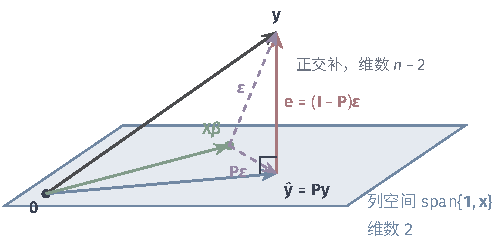
\includegraphics[width=85mm]{figures/01-basic-mathematics/05-probability-and-statistics-basics/tikz/pred-regression-projection/figure.pdf}
  \caption{简单线性回归的投影几何（示意）。$\mathbb R^n$中的平面代表设计矩阵的列空间$\operatorname{span}\{\bm 1,\bm x\}$，维数为$2$；竖直方向代表它的正交补，维数为$n-2$，图中只能画出一维。观测$\bm y=\bm X\bm\beta+\bm\varepsilon$投影为拟合值$\hat{\bm y}$；误差$\bm\varepsilon$分成列空间内的$\bm P\bm\varepsilon$（造成系数估计误差）与正交补中的$(\bm I-\bm P)\bm\varepsilon$，后者正是残差$\bm e$。}
  \label{fig:pred-regression-projection}
\end{figure}

为了计算$\mathbb E\lVert\bm e\rVert_2^2$，取正交补的一组标准正交基$\bm q_3,\dots,\bm q_n$，则$(\bm I-\bm P)\bm\varepsilon=\sum_{k=3}^n(\bm q_k^\top\bm\varepsilon)\bm q_k$，
\[
 \lVert\bm e\rVert_2^2=\sum_{k=3}^n(\bm q_k^\top\bm\varepsilon)^2.
\]
在(A2)、(A3)下，$\operatorname{Var}(\bm q_k^\top\bm\varepsilon)=\sigma^2\lVert\bm q_k\rVert_2^2=\sigma^2$，且$\mathbb E\bm q_k^\top\bm\varepsilon=0$，故$\mathbb E(\bm q_k^\top\bm\varepsilon)^2=\sigma^2$，求和得
\[
 \mathbb E\lVert\bm e\rVert_2^2=(n-2)\sigma^2.
\]
误差有$n$个分量，但其中落在列空间里的两个方向被拟合“吸收”了，留在残差中的只有$n-2$个方向。$n-2$称为残差的自由度。于是当$n>2$时，
\begin{equation}
 S^2=\frac{1}{n-2}\sum_{i=1}^ne_i^2
 \label{eq:pred-residual-variance}
\end{equation}
是$\sigma^2$的无偏估计。本节以下的$S^2$都指这个残差方差估计，它的分母是$n-2$，与单样本的修正样本方差不同。这与单样本情形的$n-1$出于同一道理：那里只拟合一个均值，列空间是$\operatorname{span}\{\bm 1\}$，失去一个自由度。

在正态假设(A4)下还能得到分布。把$\bm X$列空间的一组标准正交基$\bm q_1,\bm q_2$与$\bm q_3,\dots,\bm q_n$合起来，得到正交矩阵$\bm Q$。由第~\ref{sec:rvec-gaussian}节，$\bm\varepsilon\sim\mathcal N(\bm 0,\sigma^2\bm I)$经正交变换后$\bm Q^\top\bm\varepsilon\sim\mathcal N(\bm 0,\sigma^2\bm I)$，即$\bm q_1^\top\bm\varepsilon,\dots,\bm q_n^\top\bm\varepsilon$独立同分布于$\mathcal N(0,\sigma^2)$。因此：
\begin{itemize}
  \item $\lVert\bm e\rVert_2^2/\sigma^2=\sum_{k=3}^n(\bm q_k^\top\bm\varepsilon/\sigma)^2\sim\chi^2_{n-2}$，即$(n-2)S^2/\sigma^2\sim\chi^2_{n-2}$；
  \item $\hat{\bm\beta}=(\bm X^\top\bm X)^{-1}\bm X^\top\bm P\bm Y$只依赖$\bm P\bm Y=\bm X\bm\beta+\sum_{k=1}^2(\bm q_k^\top\bm\varepsilon)\bm q_k$，而$S^2$只依赖$\bm q_3^\top\bm\varepsilon,\dots,\bm q_n^\top\bm\varepsilon$，所以$\hat{\bm\beta}$与$S^2$独立。
\end{itemize}
这正是第~\ref{sec:samp-normal}节用正交旋转证明样本均值与样本方差独立、$(n-1)S^2/\sigma^2\sim\chi^2_{n-1}$的同一论证：单样本时列空间是$\operatorname{span}\{\bm 1\}$，只有一维；这里换成了二维。

\begin{example}[广告数据的残差方差]
\label{ex:pred-ad-residual-variance}
由例~\ref{ex:pred-ad-fit}的残差，$\sum_ie_i^2\approx2.211$，自由度$n-2=6$，$s^2\approx2.211/6\approx0.3685$，$s\approx0.607$。作为对照，$S_{yy}=26.44$是不使用$x$、只用$\bar y$拟合时的残差平方和；引入广告投入后残差平方和降到其$8.4\%$，即投入的线性变化解释了销量总波动的约$91.6\%$。
\end{example}

\subsection{回归系数的区间估计与检验}

\paragraph{标准误、$t$区间与检验}

把$\operatorname{Var}(\hat\beta_1)=\sigma^2/S_{xx}$中的$\sigma$换成$S$，得到斜率的估计标准误$\operatorname{se}(\hat\beta_1)=S/\sqrt{S_{xx}}$。在(A1)--(A4)下，$(\hat\beta_1-\beta_1)/(\sigma/\sqrt{S_{xx}})\sim\mathcal N(0,1)$，$(n-2)S^2/\sigma^2\sim\chi^2_{n-2}$，二者独立，按$t$分布的定义，
\begin{equation}
 \frac{\hat\beta_1-\beta_1}{S/\sqrt{S_{xx}}}\sim t_{n-2}.
 \label{eq:pred-slope-t}
\end{equation}
这是与单样本$t$统计量~\eqref{eq:pred-t-pivot}完全平行的枢轴量，只是自由度变为$n-2$。由此得到斜率的置信区间$\hat\beta_1\pm t_{n-2,1-\alpha/2}\,S/\sqrt{S_{xx}}$，以及$H_0:\beta_1=b$的$t$检验。最常见的是$H_0:\beta_1=0$，即均值响应不随$x$变化。截距同理，标准误为$S\sqrt{1/n+\bar x^2/S_{xx}}$。

\begin{example}[广告数据的斜率推断]
\label{ex:pred-ad-slope}
$\operatorname{se}(\hat\beta_1)=0.607/\sqrt{42}\approx0.0937$，$t_{6,0.975}\approx2.447$，斜率的$95\%$置信区间为
\[
 0.7595\pm2.447\times0.0937=[0.530,\,0.989].
\]
检验$H_0:\beta_1=0$，$t=0.7595/0.0937\approx8.11$，自由度$6$，双侧$p\approx0.0002$，拒绝$H_0$。截距的标准误为$0.607\times\sqrt{1/8+4.5^2/42}\approx0.473$，$95\%$区间为$2.432\pm2.447\times0.473\approx[1.27,\,3.59]$。截距是$x=0$即完全不投放广告时的平均销量，但数据中最小的投入是$1$万元，这个区间依赖直线在$[0,1]$上仍然成立，应当谨慎解读。
\end{example}

\paragraph{关联、效应大小与因果}

$H_0:\beta_1=0$被拒绝，说明在模型假设下，销量的均值与广告投入有线性关联。它没有说明关联有多强，这要看估计值和区间：投入每增加$1$万元，平均销量估计增加约$76$件，$95\%$置信区间约为$53$到$99$件。这才是实际决策需要的效应大小。

更重要的是，回归系数描述的是“投入较高的城市，销量平均较高”，而不是“提高投入会使销量增加”。在这批观测数据中，投入并不是随机分配的：公司很可能向市场规模大的城市投入更多，而市场规模本身就会带来更高的销量。这时$\hat\beta_1$混合了广告的作用与城市规模的作用，无论$p$值多小都无法将二者分开。若由研究者随机决定各城市的投入，城市规模等因素就与投入无关，斜率才可以解释为投入的平均因果作用。统计显著性只回答“关联是否可能由随机波动造成”，不回答“关联从何而来”。因果作用的定义与识别条件见\BookChapterRef{chap:causal-inference}{卷4《数学准备：流形、概率分布与统计推断》的“因果响应”章}。

\subsection{均值响应与新观测的预测}

\paragraph{均值响应的置信区间}

给定投入$x_0$，城市的平均销量是$\mu(x_0)=\beta_0+\beta_1x_0$，其估计为$\hat\mu(x_0)=\hat\beta_0+\hat\beta_1x_0$。利用$\hat\beta_0=\bar Y-\hat\beta_1\bar x$改写为
\[
 \hat\mu(x_0)=\bar Y+\hat\beta_1(x_0-\bar x).
\]
上面已经算出$\bar Y$与$\hat\beta_1$不相关，方差直接相加：
\begin{equation}
 \operatorname{Var}\bigl(\hat\mu(x_0)\bigr)=\frac{\sigma^2}n+(x_0-\bar x)^2\frac{\sigma^2}{S_{xx}}
 =\sigma^2\Bigl(\frac1n+\frac{(x_0-\bar x)^2}{S_{xx}}\Bigr).
 \label{eq:pred-mean-response-variance}
\end{equation}
第一项是整条直线上下平移的不确定性，第二项是斜率的不确定性在$x_0$处造成的波动，它随$x_0$与$\bar x$的距离平方增长。拟合直线像一根绕着$(\bar x,\bar Y)$转动的杆，离支点越远，摆动越大。

$\hat\mu(x_0)$是$\hat{\bm\beta}$的线性函数，在(A4)下服从正态分布并与$S^2$独立，因此
\[
 \hat\mu(x_0)\pm t_{n-2,1-\alpha/2}\,S\sqrt{\frac1n+\frac{(x_0-\bar x)^2}{S_{xx}}}
\]
是$\mu(x_0)$的置信水平为$1-\alpha$的置信区间。

\paragraph{新观测的预测区间}

若要预测投入为$x_0$的某个城市的实际销量$Y_0=\mu(x_0)+\varepsilon_0$，其中$\varepsilon_0\sim\mathcal N(0,\sigma^2)$与已有数据独立，则与第~\ref{sec:pred-prediction}节一样，预测误差$Y_0-\hat\mu(x_0)$包括新观测的噪声和估计误差两部分，方差相加：
\[
 \operatorname{Var}\bigl(Y_0-\hat\mu(x_0)\bigr)=\sigma^2\Bigl(1+\frac1n+\frac{(x_0-\bar x)^2}{S_{xx}}\Bigr).
\]
按同样的论证得到$Y_0$的预测区间
\begin{equation}
 \hat\mu(x_0)\pm t_{n-2,1-\alpha/2}\,S\sqrt{1+\frac1n+\frac{(x_0-\bar x)^2}{S_{xx}}}.
 \label{eq:pred-regression-prediction-interval}
\end{equation}
与均值区间相比，根号中多出的$1$对应新观测的噪声，不随样本量增大而消失。$x_0=\bar x$时，两种区间分别回到第~\ref{sec:pred-intervals}节的均值区间与第~\ref{sec:pred-prediction}节的预测区间的形式，只是自由度为$n-2$。

\begin{example}[投入$6$万元时的两种区间]
\label{ex:pred-ad-intervals}
取$x_0=6$，$\hat\mu(6)=2.432+0.7595\times6\approx6.989$，$(x_0-\bar x)^2/S_{xx}=2.25/42\approx0.0536$。
\begin{itemize}
  \item 均值响应：标准误$0.607\sqrt{0.125+0.0536}\approx0.257$，$95\%$置信区间$6.989\pm2.447\times0.257\approx[6.36,\,7.62]$；
  \item 新观测：标准误$0.607\sqrt{1+0.125+0.0536}\approx0.659$，$95\%$预测区间$6.989\pm2.447\times0.659\approx[5.38,\,8.60]$。
\end{itemize}
前者说投入$6$万元的城市平均销量在$636$到$762$件之间；后者给出某个投入$6$万元的城市的销量范围：$538$到$860$件，按$95\%$的预测水平构造。预测区间约为均值区间的$2.6$倍宽。
\end{example}

图~\ref{fig:pred-regression-bands}(a)把所有$x_0$处的两种区间连成两条带。均值置信带在$\bar x=4.5$处最窄，向两侧张开；预测带宽得多，且由于根号中的$1$占主导，看起来几乎是平行的。

\begin{figure*}[htbp]
  \centering
  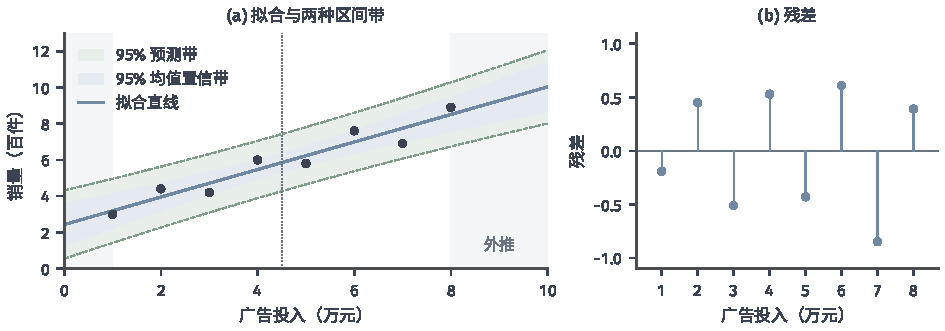
\includegraphics[width=160mm]{figures/01-basic-mathematics/05-probability-and-statistics-basics/matplotlib/pred-regression-bands/figure.pdf}
  \caption{广告数据的简单线性回归。(a) 黑点为$8$个城市的观测，蓝线为拟合直线$\hat y=2.432+0.7595x$；蓝色窄带为均值响应的$95\%$置信带，绿色宽带（虚线为边界）为新观测的$95\%$预测带，二者都由$t_{6,0.975}$与$s\approx0.607$计算。点线标出$\bar x=4.5$，置信带在此处最窄。灰色区域$x<1$与$x>8$超出了观测范围，那里的带只在直线关系继续成立时才有意义。(b) 各城市的残差，没有明显的弯曲趋势或随$x$扩大的波动。}
  \label{fig:pred-regression-bands}
\end{figure*}

\paragraph{残差检查与外推}

以上所有区间都以(A1)--(A4)为前提，而这些假设可以部分地用残差来检查。若真实关系是弯曲的，残差会随$x$呈现系统的弧形；若误差方差随$x$增大，残差的散布会呈喇叭形；个别远离其余点的残差提示异常观测。图~\ref{fig:pred-regression-bands}(b)中残差正负交替，大小没有随$x$明显变化，看不出违背假设的迹象。只有$8$个观测时，这种检查的能力很有限，只能发现明显的问题。

外推需要格外小心。取$x_0=10$，公式给出均值响应的$95\%$区间约$[8.66,\,11.39]$，预测区间约$[8.01,\,12.05]$，都比$x_0=6$时宽，这反映了式~\eqref{eq:pred-mean-response-variance}中距离项的增长。但这种加宽只计入了模型成立时的估计误差，没有计入模型本身出错的可能：数据只覆盖$1$到$8$万元，投入继续增加时，销量很可能因市场饱和而增长放缓。在观测范围之外，直线是否仍然成立，数据本身无法回答，区间公式也无从反映。

\section{本章小结}
\label{sec:pred-summary}

本章回答了章首的三个问题。对平均灌装量，我们构造了置信区间$[500.69,\,502.31]$；对“平均灌装量等于$500$”，$t$检验给出$p\approx0.002$；对下一瓶，预测区间为$[498.81,\,504.19]$。三个结果使用同一批数据和同一个抽样分布理论，却回答不同的问题。表~\ref{tab:pred-summary}按目标对象、所用随机性、构造依据和概率含义把它们并列比较。

\begin{table*}[htbp]
  \centering
  \begin{tabularx}{\linewidth}{@{}p{0.12\linewidth}XXXX@{}}
    \toprule
    方法 & 目标对象 & 随机性来源 & 构造依据 & 概率含义\\
    \midrule
    置信区间 & 固定的未知参数 & 样本在重复抽样中的变化 & 枢轴量的抽样分布 & 规则以$1-\alpha$的概率覆盖真参数\\
    可信区间 & 参数 & 给定数据时参数的后验分布 & 先验与似然得到的后验 & 参数落在区间中的后验概率为$1-\alpha$\\
    假设检验 & 关于参数的陈述 & 原假设下样本的变化 & 原假设下统计量的分布 & $H_0$为真时错误拒绝的概率不超过$\alpha$\\
    预测区间 & 未来的单个观测 & 样本与新观测的联合变化 & 新观测与估计量之差的分布 & 区间以$1-\alpha$的概率覆盖新观测\\
    \bottomrule
  \end{tabularx}
  \caption{本章四类推断方法的比较。前三类的对象都是参数，预测区间的对象是随机变量；可信区间的概率对参数计算，其余三类的概率对样本计算。}
  \label{tab:pred-summary}
\end{table*}

区间估计的共同方法是从枢轴量反解参数。正态模型下的均值$t$区间与方差卡方区间是精确的；均值区间在一般总体下还有中心极限定理提供的渐近保证，方差区间则完全依赖正态性。比例的区间面临离散性：Wald区间在小样本与边界附近覆盖不足，Clopper--Pearson区间以保守为代价保证覆盖。可信区间给出关于参数的直接概率陈述，但它的频率覆盖率取决于先验是否恰当。

假设检验先在原假设下控制第一类错误，再由效应大小、噪声与样本量决定功效。$p$值报告证据的强度，但它既不是原假设为真的概率，也不衡量效应的大小；不拒绝原假设也不证明它成立。同一族检验与同一族置信区间互为反演，只有构造规则匹配时，才能用区间直接判断检验。配对与独立设计、等方差与否、精确与近似计算，都会改变检验的结论。

预测的对象是随机变量，误差由新观测的噪声和参数估计误差两部分组成。增加样本只能减少后者，所以预测区间的半宽因子$\sqrt{1+1/n}$始终不小于$1$，而均值区间的$1/\sqrt n$趋于零。后验预测分布把这两部分写成一个积分，同样包含观测噪声与参数后验方差。

简单线性回归把以上任务放进一个模型：最小二乘给出系数，投影几何说明残差有$n-2$个自由度并给出$\sigma^2$的无偏估计，斜率的$t$区间与检验刻画线性关联，均值响应区间与预测区间分别回答“平均是多少”和“下一个是多少”。回归的显著性不等于因果，区间公式也不覆盖观测范围以外的模型误差。这些结论依赖的假设，需要用残差与研究设计来检验。

